
\documentclass[10pt]{article} % For LaTeX2e
% \usepackage{tmlr}
% If accepted, instead use the following line for the camera-ready submission:
\usepackage[accepted]{tmlr}
% To de-anonymize and remove mentions to TMLR (for example for posting to preprint servers), instead use the following:
%\usepackage[preprint]{tmlr}

% Optional math commands from https://github.com/goodfeli/dlbook_notation.
\input{math_commands.tex}
%%%%%%%%%%%%%%%%%%%%%%%%%%%%%%%%%%%%%%%%%%%%%%%%%
% CUSTOM COMMANDS AND PACKAGES
%%%%%%%%%%%%%%%%%%%%%%%%%%%%%%%%%%%%%%%%%%%%%%%%%
%\usepackage{apacite}
\usepackage{natbib}
\setcitestyle{numbers,square}
\usepackage{url}
\usepackage[utf8]{inputenc} % allow utf-8 input
\usepackage[T1]{fontenc}    % use 8-bit T1 fonts
\usepackage{hyperref}       % hyperlinks
\usepackage{url}            % simple URL typesetting
\usepackage{booktabs}       % professional-quality tables
\usepackage{amsfonts}       % blackboard math symbols
\usepackage{amsthm}
\usepackage{nicefrac}       % compact symbols for 1/2, etc.
\usepackage{microtype}      % microtypography
\usepackage{xcolor}         % colors

\usepackage{bbding}
\usepackage{pifont}
\usepackage{wasysym}
\usepackage{amssymb}

%\newtheorem{lemma}{Lemma}
\usepackage{sidecap}
\usepackage{wrapfig}
\usepackage{graphicx}
\usepackage{lipsum}
\usepackage{algorithmic}
\usepackage{algorithm}
\usepackage{ragged2e}
\usepackage{multirow}
\usepackage{epigraph}
%\usepackage[table]{xcolor}
%%%%%%%%%%%%%%%%%%%%%%%%%%%%%%%%%%%%%%%%%%%%%%%%%
% CUSTOM COMMANDS AND PACKAGES
%%%%%%%%%%%%%%%%%%%%%%%%%%%%%%%%%%%%%%%%%%%%%%%%%
% \usepackage{pslatex}
    
    
% if you use cleveref..
%\usepackage[capitalize,noabbrev]{cleveref}

\title{Delving into Semantic Scale Imbalance}


% Authors must not appear in the submitted version. They should be hidden
% as long as the tmlr package is used without the [accepted] or [preprint] options.
% Non-anonymous submissions will be rejected without review.
%\iffalse
\author{\name Yanbiao Ma\textsuperscript{1}, Licheng Jiao\textsuperscript{1}, Fang Liu\textsuperscript{1}, Yuxin Li\textsuperscript{2}, Shuyuan Yang\textsuperscript{1}, Xu Liu\textsuperscript{1} \\
        \email \{miao.xiong, shen.li\}@u.nus.edu, wenjie.feng@nus.edu.sg, ailin@u.nus.edu, \{jihai, bhooi\}@comp.nus.edu.sg \\
      \addr \textsuperscript{1} Institute of Data Science, National University of Singapore \\
      \textsuperscript{2} Department of Computer Science, National University of Singapore
}
%\fi \normalsize

\author{\setlength{\baselineskip}{12.5pt}{\name Yanbiao Ma, Licheng Jiao, Fang Liu, Yuxin Li, Shuyuan Yang, Xu Liu \\
      \addr \normalsize Key Laboratory of Intelligent Perception and Image Understanding of the Ministry of Education \\ 
      \normalsize Xidian University \\
      \normalsize Xi’an, 710071, China \\
      \email \normalsize \{ybmamail,yxli\_12\}@stu.xidian.edu.cn, lchjiao@mail.xidian.edu.cn, \\ f63liu@163.com, syyang@xidian.edu.cn, xuliu361@163.com 
}}

\iffalse
\author{Yanbiao Ma \& Licheng Jiao \& Fang Liu \& Yuxin Li  \& Shuyuan Yang  \& Xu Liu \\
Key Laboratory of Intelligent Perception and Image Understanding of the Ministry of Education\\
Xidian University\\
Xi’an, 710071, China \\
\texttt{\{ybmamail,yxli\_12\}@stu.xidian.edu.cn, lchjiao@mail.xidian.edu.cn,}  \\
\texttt{f63liu@163.com, syyang@xidian.edu.cn, xuliu361@163.com} 
}
\fi

% The \author macro works with any number of authors. Use \AND 
% to separate the names and addresses of multiple authors.

\newcommand{\fix}{\marginpar{FIX}}
\newcommand{\new}{\marginpar{NEW}}

\def\month{08}  % Insert correct month for camera-ready version
\def\year{2022} % Insert correct year for camera-ready version
\def\openreview{\url{https://openreview.net/forum?id=p5V8P2J61u}} % Insert correct link to OpenReview for camera-ready version

% \theoremstyle{definition}
\newtheorem{defn}{Definition}[section]
\newtheorem{thm}{Theorem}[section]
\newtheorem{prop}{Proposition}[section]
\newtheorem{proposition}{Proposition}
\newtheorem{definition}{Definition}
\newtheorem{theorem}{Theorem}
\newtheorem{corollary}{Corollary}
\newtheorem{problem}{Problem}
\newtheorem{remark}{Remark}


%%%%%%%%%%%%%%%%%%%%%%%%%%%%%%%%
% THEOREMS
%%%%%%%%%%%%%%%%%%%%%%%%%%%%%%%%
% \theoremstyle{plain}
% \newtheorem{theorem}{Theorem}[section]
% \newtheorem{proposition}[theorem]{Proposition}
\newtheorem{lemma}[theorem]{Lemma}
% \newtheorem{corollary}[theorem]{Corollary}
\theoremstyle{definition}
% \newtheorem{definition}[theorem]{Definition}
\newtheorem{assumption}[theorem]{Assumption}
\theoremstyle{remark}
% \newtheorem{remark}[theorem]{Remark}


% note tools
\newcommand{\hide}[1]{}
% \newcommand{\note}[1]{{\textsf{\textcolor{blue}{[#1]}}}}
\newcommand{\todo}[1]{{\textsf{\textcolor{blue}{{\textsf{REVISE}: \em [#1]}}}}}
\newcommand{\reminder}[1]{{\textsf{\textcolor{red}{[#1]}}}}
\newcommand{\atn}[1]{\textcolor{red}{#1}}
\newcommand{\notice}[1]{\textcolor{blue}{#1}}


% \DeclarePairedDelimiter{\ceil}{\lceil}{\rceil}

\definecolor{babyblueeyes}{rgb}{0.19, 0.55, 0.91}


\newcommand{\method}{\textsc{NeighborAgg}\xspace}  %LNAS, LeNAS
\newcommand{\methodcmd}{\textsc{NeighborAgg-CMD}\xspace}  %LNAS-CMD, LeNAS-CMD


\newcommand{\predonly}{\textit{ProbOnly}\xspace}
\newcommand{\neionly}{\textit{NeighOnly}\xspace}

\newcommand{\kdtree}{KD-tree\xspace}
\newcommand{\trustscore}{trustworthiness score\xspace}
\newcommand{\jiangtrustscore}{Trust Score\xspace}
\newcommand{\mislabtsk}{mislabel detection task\xspace}
\newcommand{\aggoperator}{\textsc{Agg}\xspace}



% \renewcommand{\algorithmicrequire}{\textbf{Input:}}
% \renewcommand{\algorithmicensure}{\textbf{Output:}}
\newcommand{\ReturnN}[1]{\State \textbf{return} #1}
\newcommand{\StatexPar}[2]{\Statex #1 \textcolor{babyblueeyes}{\textit{// #2}}} % lightgray
\newcommand{\linecomment}[1]{\textcolor{babyblueeyes}{\textit{$\triangleright$ #1}}}






\begin{document}

\maketitle


\fancyhead[L]{Published as a conference paper at ICLR 2023}

%\setlength{\baselineskip}{12.5pt}

\begin{abstract}
Model bias triggered by long-tailed data has been widely studied. However, measure based on the number of samples cannot explicate three phenomena simultaneously: \textbf{(1)} Given enough data, the classification performance gain is marginal with additional samples. \textbf{\!(2)} Classification performance decays precipitously as the number of training samples decreases when there is insufficient data. \textbf{(3)} Model trained on sample-balanced datasets still has different biases for different classes. In this work, we define and quantify the semantic scale of classes, which is used to measure the feature diversity of classes. It is exciting to find experimentally that there is a marginal effect of semantic scale, which perfectly describes the first two phenomena. Further, the quantitative measurement of semantic scale imbalance is proposed, which can accurately reflect model bias on multiple datasets, even on sample-balanced data, revealing a novel perspective for the study of class imbalance. Due to the prevalence of semantic scale imbalance, we propose semantic-scale-balanced learning, including a general loss improvement scheme and a dynamic re-weighting training framework that overcomes the challenge of calculating semantic scales in real-time during iterations. Comprehensive experiments show that dynamic semantic-scale-balanced learning consistently enables the model to perform superiorly on large-scale long-tailed and non-long-tailed natural and medical datasets, which is a good starting point for mitigating the prevalent but unnoticed model bias. In addition, we look ahead to future challenges.
\end{abstract}

\section{Introduce}

In practical tasks, long-tailed class imbalance is a common problem, and the imbalance in number makes the trained model easily biased towards the dominant head classes and perform poorly on the tail classes \cite{paper1,paper2}. However, what is overlooked is that, in addition to long-tailed data, our study finds that the model trained on sample-balanced data still shows different biases for different classes. This model bias is not taken into account by the study for class imbalance problem, and it cannot be ameliorated by the current methods proposed for long-tailed data \cite{paper3,paper4,paper5,paper6}. For natural datasets, classes artificially divided by different semantic concepts correspond to different semantic scales, which can lead to different degrees of optimization when the deep metric is a single scale \citep{paper23}. In this study, we attempt to uncover more information from the data itself and introduce and quantify the semantic scale imbalance for representing more general model bias. The semantic-scale-balanced learning is further proposed, which is used to improve loss to mitigate model bias.


The classes corresponding to different semantic concepts have different feature diversity, and we equate the diversity to the semantic scale. Usually, the finer the semantic concept of a class label, the less rich the feature diversity, the less information a model can extract, and the worse the model performs on that class \cite{paper14,paper23,paper13,paper19,paper20,paper21}. The manifold distribution hypothesis \cite {paper7} states that a specific class of natural data is concentrated on a low-dimensional manifold. The larger the range of value variation along a specific dimension of the manifold, such as illumination and angle, the richer the feature and the larger the volume of the manifold. For example, in Figure \ref{fig1}, since "Swan" is a subclass of "Bird", its semantic concept is finer, so the feature diversity of "Bird" is richer than that of "Swan", and the corresponding volume of manifold is larger. 


Obviously, the semantic scale can be measured by the volume of manifold. We present a reliable and numerically stable quantitative measurement of the semantic scale and further define the semantic scale imbalance. To avoid confusion, we refer to the volume of the manifold calculated on the sample space as the sample volume and the feature space as the feature volume. In addition, our innovative study for semantic scale imbalance can simultaneously and naturally explain the following two phenomena that cannot be explicated by existing studies of class imbalance:

 \textbf{(1)} As the number of samples increases linearly, the model performance shows a trend of rapid improvement in the early stages and leveling off in the later stages \cite {paper22}. 
 
 \textbf{(2)} Even models trained on the dataset with balanced sample numbers still suffer from class bias.


\begin{wrapfigure}[31]{r}{21.5em} % 纵向8行,图片靠右,宽度12.5em
\begin{center}
\vskip -0.25in
\includegraphics[width=0.45\columnwidth]{fig1}
\vskip -0.1in
\caption{The features from "Bird" mapped by CNNs are concentrated on a low-dimensional manifold, and the three-color point sets represent the three sub-classes of "Bird". Among them, the \textcolor[RGB]{255,94,30}{orange} point set represents "Swan", whose feature volume is obviously smaller than that of "Bird". The classification experiments on sample-balanced datasets show that the models are biased towards the classes with larger semantic scales, such as the decision surface shown by the \textcolor[RGB]{112,173,71}{green} line. In this case, the re-weighting strategy based on the number of samples does NOT work, while our proposed re-weighting approach based on the semantic scale biases the decision surface toward the class with a larger feature volume (\textcolor[RGB]{255,0,0}{red} line).}
%\vskip -0.03in
\label{fig1}
\end{center}
\end{wrapfigure}
%\exercise

The experiments demonstrate that semantic scale imbalance is more widely present in natural datasets than sample number imbalance, allowing the study scope for class imbalance to be extended to arbitrary datasets. Then, how to mitigate the adverse effects of semantic scale imbalance? We are inspired by classification methods for long-tailed data, and current solutions for class imbalance problem usually adopt re-sampling strategies \cite{paper8,paper10,paper12} and cost-sensitive learning \cite{paper16,paper17,paper18}. However, re-sampling may either introduce a large number of duplicate samples, making the model susceptible to overfitting when oversampling, or discard valuable samples when undersampling. Therefore by drawing on the classical re-weighting strategy \cite {paper24}, we propose the dynamic semantic-scale-balanced learning. Its core idea is to dynamically rather than invariably measure the degree of imbalance between semantic scales in the feature space, to achieve a dynamic evaluation of the weaker classes and assign greater weights to their corresponding losses.


In this work, our \textbf{key contributions} are summarized as:


\textbf{(1)} We propose the novel idea of leveraging the volume of manifold to measure the semantic scale (Sec \ref{3.2}). It is also innovative to find that the semantic scale has the marginal effect (Sec \ref{3.3}), and that the semantic scale of the dataset is highly consistent with model performance in terms of trends.

\textbf{(2)} We introduce and define semantic scale imbalance, aiming to measure the degree of class imbalance by semantic scale rather than sample number, which reveals a new perspective for the study of class imbalance problem. Experiments show that semantic scale imbalance is prevalent in the dataset and can more accurately reflect model bias that affects model performance (Sec \ref{3.4}).

\textbf{(3)} Semantic-scale-balanced learning is proposed to mitigate model bias, which includes a general loss improvement scheme (Sec \ref{4.1}) and a dynamic re-weighting training framework (Sec \ref{4.2}) that overcomes the challenge of calculating semantic scales in real-time during iterations. Comprehensive experiments demonstrate that semantic-scale-balanced learning is applicable to a variety of datasets and achieves significant performance gains on multiple vision tasks (Sec \ref{5}).

\section{Slow Drift Phenomenon of Features and Marginal Effect\label{2}}


Since the model parameters are changing during training, \cite {paper25} studies the drifting speed of embeddings by measuring the difference in features of the same instance across training iterations. Experiments on the Stanford Online Products (SOP) dataset \cite {paper83} show that the features change drastically in the early stage of training, become relatively stable after traversing the dataset twice, and drift gets extremely slowly when the learning rate decreases. This ensures that it is reasonable to leverage historical features to calculate semantic scales.

Marginal effect \cite {paper14} describes that in the early stages of model training, the network is able to learn features quickly, but since there is information overlap among samples, as the number of samples increases, the information of data will gradually saturate and the improvement in model performance from newly added samples will diminish. The effective number of samples is proposed to represent the information of data, but its limitation is that it does not work when the number of samples for each class is balanced.

Assume that the volume of each sample is unit volume $1$ and define the set of all samples for a class as $\Omega$ with volume $N$ and $N\!\!\ge\!\!1$. A new sample may overlap with a previous sample such that the probability of overlap is $P$ and that of non-overlap is $1\!\!-\!\!P$. As the information of data increases, the probability $P$ will be higher. 

Define the effective number of samples as ${E_n}$, and ${E_n} = 1 + \beta \frac{{1 - {\beta ^{n - 1}}}}{{1 - \beta }} = \frac{{1 - {\beta ^n}}}{{1 - \beta }}$ \cite {paper14}, where $n$ denotes the number of samples, hyperparameter $\beta = \frac{{N - 1}}{N} \in [ {0,1} )$ controls how fast ${E_n}$ grows as $n$ increases. When $N = 1$, $\beta  = 0$ and ${E_n}= 1$, meaning that all samples can be represented by a single prototype via data augmentation. When $N \to \infty $, $\beta  \to 1$, implying that there is no overlapping, then $\mathop {\lim }\limits_{\beta  \to 1 } \!\!\frac{{1 - {\beta ^n}}}{{1 - \beta }} \!\!= \!\!\mathop {\lim }\limits_{\beta  \to 1 } \!\!\frac{{{{\left( {1 - {\beta ^n}} \right)}^\prime }}}{{{{\left( {1 - \beta } \right)}^\prime }}} \!\!= \!\!\mathop {\lim }\limits_{\beta  \to 1 } \!\!\frac{{ - n{\beta ^{n - 1}}}}{{ - 1}} \!\!= \!\!n$, which indicates that the effective number of samples does not increase faster than the number of samples, but this is not the case in our experimental results.

The effective number of samples ${E_n}$ is an exponential function of the number of samples $n$. The hyperparameters $\beta$ corresponding to classes of different grain should be different. However, the selection of $\beta$ requires more information from the data itself, but this problem is not addressed by \cite {paper14}, which is forced to assume that $\beta$ is the same for all classes. In this case, compared to the number of samples, ${E_n}$ simply uses the exponential function to obtain smoother weights. Furthermore, when the number of samples is balanced, ${E_n}$ is the same for each class and cannot be used to mitigate model bias, so we attempt to mine the data for information (or feature diversity) of each class to facilitate the study of imbalance problem.


\section{Semantic Scale Imbalance}
In this section, first, sample volume, feature volume, and semantic scale imbalance are defined. Next, we derive a quantitative measurement of feature volume to measure the semantic scale from the perspective of singular value decomposition of the data matrix and information theory. Then, the marginal effect of semantic scale is investigated. Finally, we discuss the relationship between semantic scale imbalance and model bias.
\subsection{Definitions}

Different semantic concepts correspond to different semantic scales, for example, the scale of "Bird" is larger than that of "Swan". For each class, we equate its feature diversity to its semantic scale and measure the semantic scale by the volume of subspace spanned by samples or features. Deep neural networks can be viewed as a combination of a feature mapping function $f({x,\theta})$ and a trained downstream classifier $g(z)$, i.e., $x\to z( \theta )\to y$. Let the samples of a class be $X=[ {{x_1},{x_2}, \ldots ,{x_m}} ]$, and the embeddings learned by deep neural networks are represented as $Z = \left\{ {{z_i}|{z_i} = f( {{x_i},\theta } ) \in {\mathbb{R}^d},i = 1,2, \ldots ,m} \right\}$.

\textbf{Definition 3.1.} (Sample volume) The volume of the subspace spanned by sample set $X$.

\textbf{Definition 3.2.} (Feature volume) The volume of the subspace spanned by feature vectors $Z$.

\textbf{Definition 3.3.} (Semantic scale imbalance) A phenomenon of imbalance in the size of semantic scales measured by sample volume or feature volume.



\subsection{Quantification of Semantic Scale\label{3.2}}
Given the data $X=[ {{x_1},{x_2}, \ldots ,{x_m}} ]$ and the learned embeddings $Z = \left[ {{z_1},{z_2}, \ldots ,{z_m}} \right] \in {\mathbb{R}^{d \times m}},{z_i} = f( {{x_i},\theta } ) \in {\mathbb{R}^d},i = 1,2, \ldots ,m$, the volume of subspace spanned by the random vector ${z_i}$ (i.e., the feature volume) is derived below, and the sample volume can be calculated in the same way (Appendix \ref{C}). The covariance matrix of random vector ${z_i}$ is estimated as $ \Sigma = E\!\left[ {\frac{1}{m}\!\sum\limits_{j = 1}^m {{z_j}z_j^T} } \right] = \frac{1}{m}\!Z\!{Z^T} \in {\mathbb{R}^{d \times d}}$, ${\lambda _1} \ge {\lambda _2} \ge  \cdots  \ge {\lambda _d} > 0$ are the eigenvalues of real symmetric matrix. The singular value decomposition (SVD) of $Z$ yields $Z = U\Sigma {V^T}$ and the singular values are ${\sigma _j} = \sqrt {{\lambda _j}} ,j = 1,2, \ldots ,d$. The volume of the space spanned by the vector ${z_i}$ is proportional to the product of all singular values of the feature matrix $Z$, i.e., $V\!ol( Z ) \propto \prod\limits_{j = 1}^d {{\sigma _j}}  = \sqrt {\prod\limits_{j = 1}^d {{\lambda _j}} }$. After the determinant expansion, the characteristic polynomial of the matrix $\Sigma$ is $\Phi ( \lambda ) =  \det ( {\lambda I - \Sigma } ) ={\lambda ^d} - ({{a_{11}}+{a_{22}}+ \cdots {a_{dd}}}){\lambda ^{d - 1}} +  \cdots  + {( { - 1} )^d}\det\! \Sigma$, and ${\lambda _1}{\lambda _2} \cdots {\lambda _d} = \det\! \Sigma $. Therefore, the volume of the space spanned by the vector ${z_i}$ is proportional to the square root of the determinant of the covariance matrix of $Z$:
\begin{equation}
V\!ol( Z ) \propto \sqrt {\det ( {\frac{1}{m}\!Z\!{Z^T}} )}. 
\end{equation}The same result can be derived from the volume of a parallel hexahedron defined by vectors (Appendix \ref{E}). Considering that real-world metric tools typically have a dynamic range, for example, a ruler always has multiple scales (1mm, 1cm, or even 10cm) to measure objects of different scales, we expect the quantitative measurement of feature volume to have a multi-scale metric and therefore use the sphere packing method \cite{paper26,paper27}, which is normally adopted in information theory, to implement it.



There is an error at the boundary when filling with hyperspheres because all spheres cannot be exactly tangent to the edges of the manifold. The error of the finite feature vectors is assumed to be independent additive Gaussian noise \cite{paper26} : ${z_i}^\prime  = {z_i} + {w_i}$, where ${w_i} \sim N( {0,\frac{{{\varepsilon ^2}}}{n}I} )$ (n is the space dimension). The estimate of the number of spheres of radius $\varepsilon$ needed to pack the space spanned by all vectors is ${N_\varepsilon }{\rm{ = }}{{V\!ol\left( {Z'} \right)} \mathord{\left/{\vphantom {{V\!ol\left( {Z'} \right)} {V\!ol\left( w \right)}}} \right.\kern-\nulldelimiterspace} {V\!ol\left( Ball \right)}}$. The adjustment of the metric scale can be achieved by tuning the radius $\varepsilon$ of the spheres, thus controlling the measurement result of feature volume. Then the covariance matrix of the vector ${z_i}$ is $\Sigma ' = \frac{{{\varepsilon ^2}}}{n}I + \frac{1}{m}Z\!{Z^T} \in {\mathbb{R}^{d \times d}}$, such that $V\!ol( {Z'} ) \propto \sqrt {\det ( {\frac{{{\varepsilon ^2}}}{n}I + \frac{1}{m}Z\!{Z^T}} )} $ and $V\!ol( Ball ) \propto \sqrt {\det ( {\frac{{{\varepsilon ^2}}}{n}I} )}$. The feature volume is proportional to ${N_\varepsilon }$:
\begin{equation}
\begin{aligned}
V\!ol\left( Z \right) \propto {N_\varepsilon } &= \frac{{V\!ol\left( {Z'} \right)}}{{V\!ol\left( Ball \right)}} = \sqrt {\frac{{\det \left( {\frac{{{\varepsilon ^2}}}{n}I + \frac{1}{m}Z\!{Z^T}} \right)}}{{\det \left( {\frac{{{\varepsilon ^2}}}{n}I} \right)}}}  \\ 
&= \sqrt {\det \left( {I + \frac{n}{{m{\varepsilon ^2}}}Z\!{Z^T}} \right).} 
\end{aligned}
\end{equation}The dimension of feature ${z_i}$ is $d$, so let $n=d$. In order to increase the numerical stability, we perform a logarithmic transformation of the above equation, which does not affect the monotonicity of the function, and we can obtain $V\!ol\left( Z \right) \propto {\log _2}\sqrt {\det \left( {I + \frac{n}{{m{\varepsilon ^2}}}Z\!{Z^T}} \right)}  = \frac{1}{2}\log \det \left( {I + \frac{d}{{m{\varepsilon ^2}}}Z\!{Z^T}} \right)$. In practical training, it is essential to normalize the feature vectors so that their mean value is $0$. In this work, we set $\varepsilon=1000$, and the value of $\varepsilon$ does not affect the relative size of the space spanned by feature vectors of each class. The volume of the space spanned by $Z$ can be can be written as:
\begin{equation}
V\!ol( Z ) = \frac{1}{2}{\log _2}\det ( {I + \frac{d}{m}( {Z - {Z_{mean}}} ){{( {Z - {Z_{mean}}} )}^T}} ),
\end{equation}

where $Z_{mean}$ is the mean value of $Z$, $V\!ol( Z )>0$ when the number of samples $m>1$. We measure the semantic scale $S'$ by the feature volume, i.e., $S' = V\!ol( Z )$, and the larger $S'$, the richer the feature diversity, which we verify in Appendix \ref{Experiments on Stanford point cloud manifolds} using multiple Stanford point cloud manifolds. 

\subsection{Marginal Effect of Semantic Scale\label{3.3}}

\begin{wrapfigure}[29]{r}{21em} % 纵向8行,图片靠右,宽度12.5em
\begin{center}
\vskip -0.32in
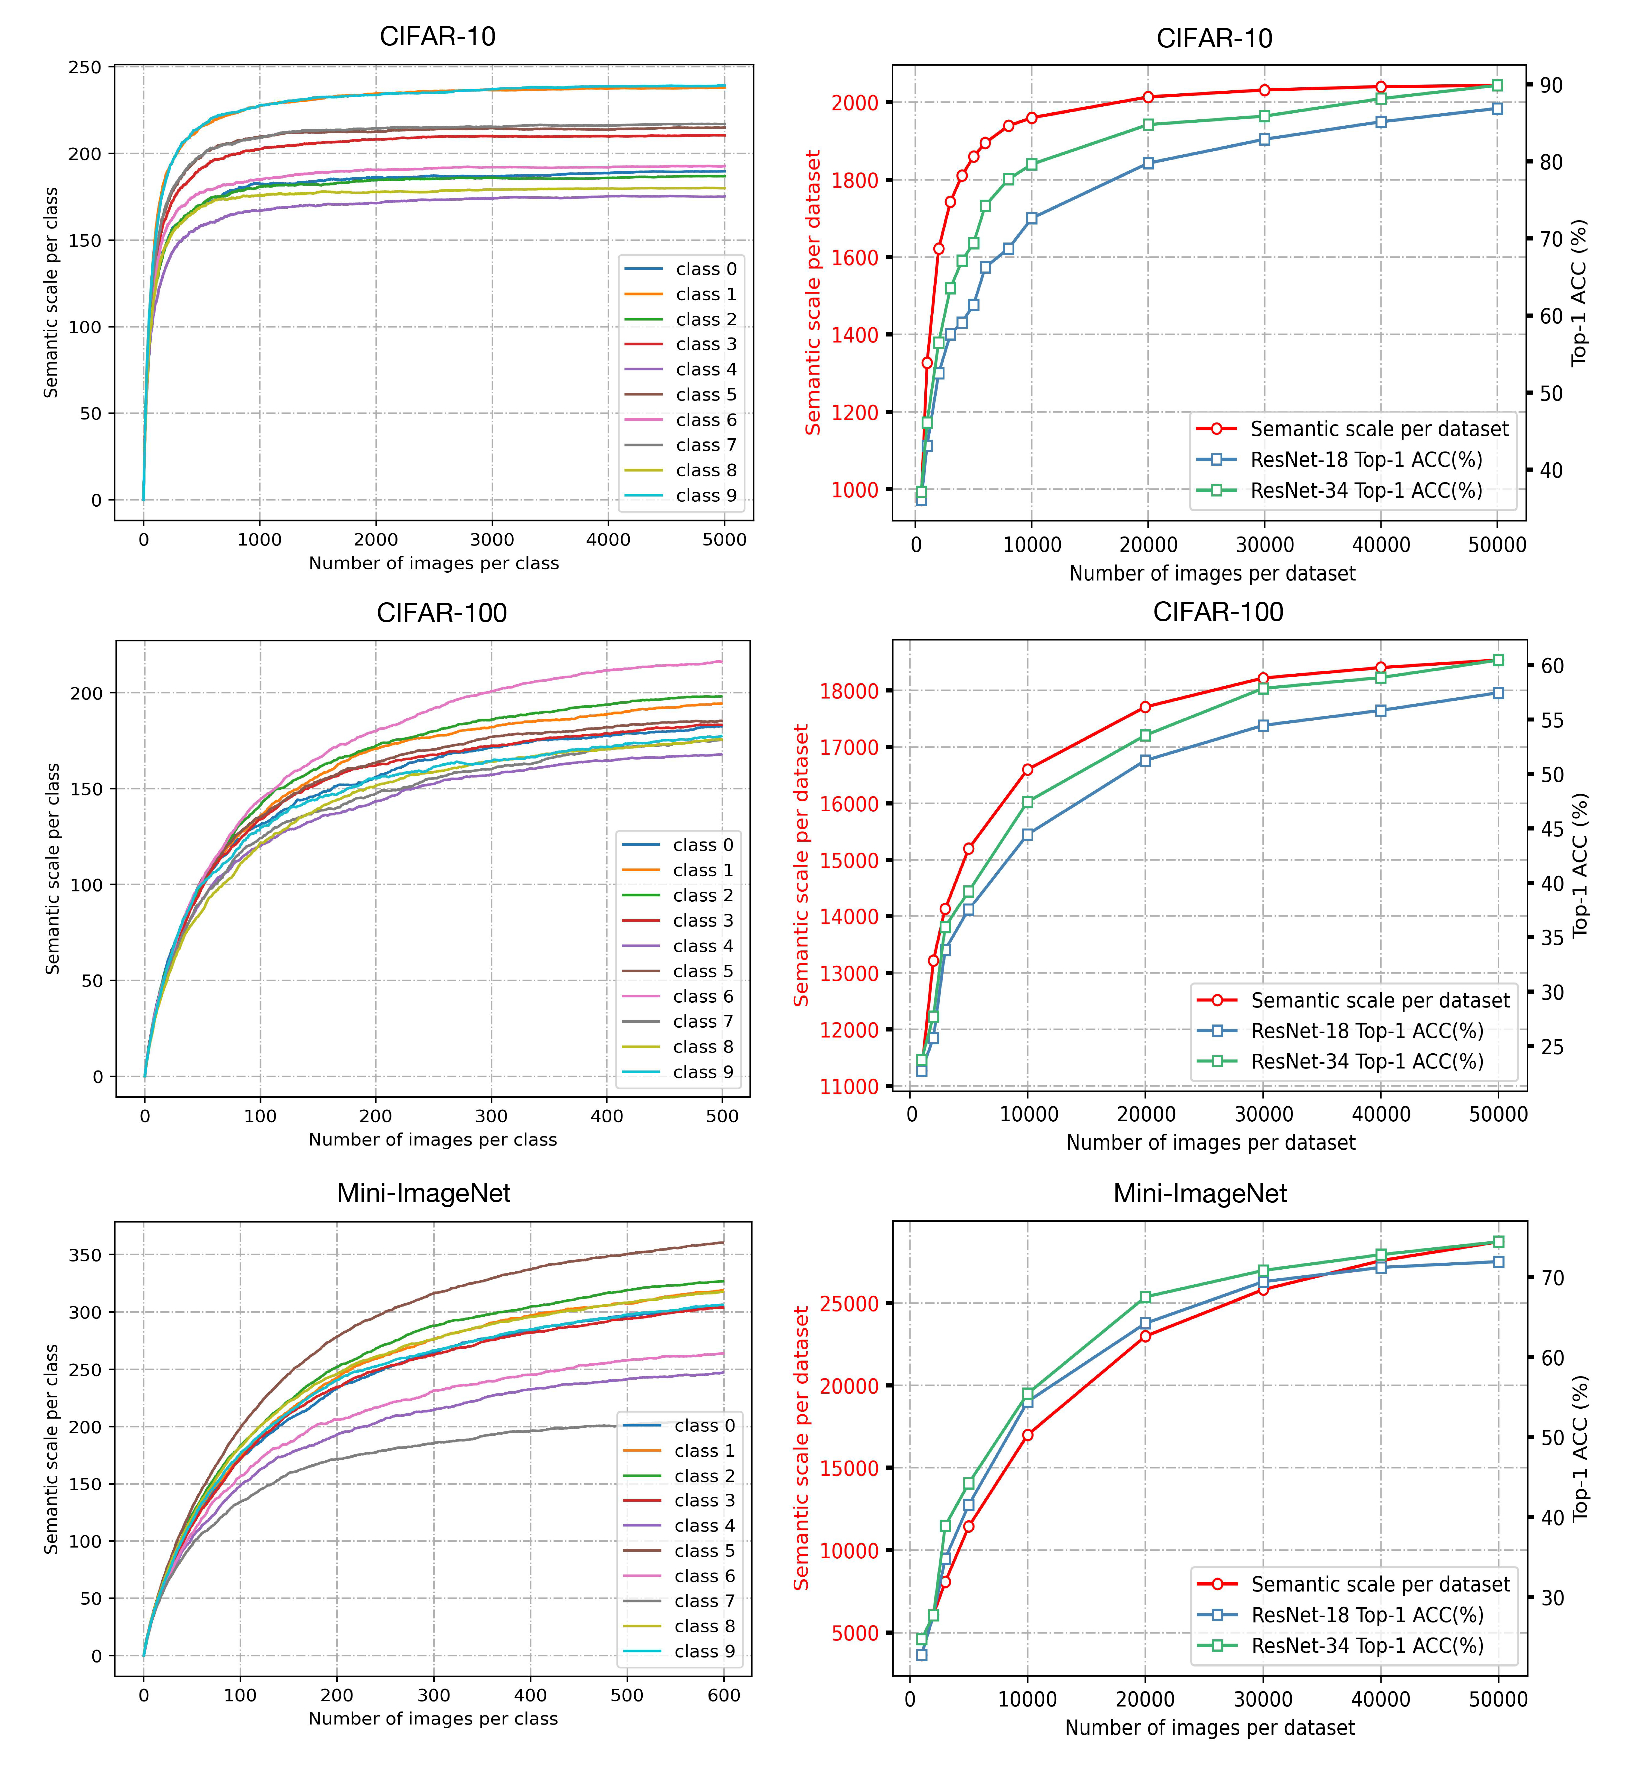
\includegraphics[width=0.47\columnwidth]{figure2}
\vskip -0.14in
\caption{\textbf{Left column}: curves of semantic scales with increasing number of samples for the first ten classes from different datasets. \textbf{Right column}: for different sub-datasets, curves of the sum of semantic scales for all classes and top-1 accuracy curves of trained ResNet-18 and ResNet-34. All models are trained using the Adam optimizer \cite {paper33} with an initial learning rate of 0.01 and then decayed by 0.98 at each epoch.}
\label{fig2}
\end{center}
\end{wrapfigure}
%\exercise

The marginal effect describes that the feature richness will gradually saturate as the number of samples increases, so the change of semantic scale should also conform to the marginal effect. Figure \ref{fig2} illustrates that as the number of samples increases, the semantic scale $S'$ measured by sample volume gradually saturates, which indicates that the quantitative measurement of semantic scale is as expected. In addition, the growth rate of the semantic scale varies across classes, which is determined by the grain size of the class itself. It leads to different semantic scales even if all classes have the same number of samples.

To investigate why adding samples has a marginal improvement in model performance when the training samples are sufficient, we use the following method to generate new training datasets for classification experiments: assume that the total number of classes in the original dataset is $C$, and $m$ samples are randomly selected from each class to form a sub-dataset with a total number of samples of $C \times m$. The sub-datasets generated based on CIFAR-10, CIFAR-100 \cite {paper28} and Mini-ImageNet \cite {paper31} are shown in Appendix \ref{B.1}.


We train ResNet-18 and ResNet-34 \cite {paper32} on each of the \textbf{31} training sets in Table \ref{table6}, and the sum of the semantic scales for all classes and the corresponding top-1 accuracy are shown in Figure \ref{fig2}. We are pleasantly surprised to find that when the semantic scale increases rapidly, the model performance improves swiftly with it, and when the semantic scale becomes saturated, the improvement is small.


\subsection{Semantic Scale Imbalance and Model Bias \label{3.4}}
\subsubsection{Quantification of Semantic Scale Imbalance}

\begin{table}[h]
\renewcommand\arraystretch{1.3}
\vskip -0.15in
\setlength{\tabcolsep}{6pt} %修改边距
\caption{Pearson correlation coefficients between the accuracy of classes and the semantic scales $S$ with different $\alpha$. $N$ denotes the number of samples, and $S'$ represents the semantic scale without considering inter-class interference. $E_n$ denotes the number of effective samples.}
\label{table1}
\vskip 0.03in
\centering  
\begin{small}
\begin{tabular}{l|c|c|c|c|c|ccccc }
\hline \toprule
\multirow{2}{*}{Dataset}    & \multirow{2}{*}{Model}   & \multirow{2}{*}{$N$} & \multirow{2}{*}{$E_n$} & \multirow{2}{*}{$W$}  &  \multirow{2}{*}{$S'$}  &\multicolumn{5}{c}{$S$}   \\ \cline{7-11}
       & & & & & &$\alpha$=1  &$\alpha$=1.5  &$\alpha$=2   &$\alpha$=2.5   &$\alpha$=3 \\  \hline
\multirow{2}{*}{CIFAR-10-LT}  & ResNet-18 & 0.8346 &0.8664 &0.2957 & 0.8688 & 0.8456 & \textbf{0.9603} & 0.9553  & 0.9398 & 0.9269 \\
  & ResNet-34 & 0.7938 &0.8476 &0.3186 & 0.9426 & 0.7950 & 0.9678  & \textbf{0.9884} & 0.9854 & 0.9796 \\  \hline
\multirow{2}{*}{CIFAR-10} & ResNet-18 & 0.0950 &0.0950 & 0.1743 & 0.5433 &\textbf{0.7850} & 0.7250  & 0.6644 & 0.6060 & 0.5607 \\
  & ResNet-34 & 0.1502 &0.1502 & 0.2075 & 0.5750 & \textbf{0.8056} & 0.7442 & 0.6870  & 0.6465 & 0.5906 \\
\bottomrule \hline
 \end{tabular}
 \end{small}
\vskip -0.05in
\end{table}

The previous subsection shows that the sum of semantic scales for all classes in the dataset is highly correlated with the model performance, and we further investigate the relationship between semantic scale and model bias for different classes. When a class is closer to other classes, the model performs worse on that class \cite{paper34,paper44}. Therefore, inter-class interference is additionally considered when quantifying the degree of imbalance between semantic scales of classes. When class $i$ is closer to other classes, a smaller weight ${w_i}$ is applied to the semantic scale of class $i$.


Specifically, the semantic scale of $m$ classes after maximum normalization is assumed to be $S' = {\left[ {{S'_1},{S'_2}, \ldots ,{S'_m}} \right]^T}$, and the centers of all classes are $O = {\left[ {{o_1},{o_2}, \ldots ,{o_m}} \right]^T}$. Define the distance between the centers of class $i$ and class $j$ as ${d_{i,j}} = {\left\| {{o_i} - {o_j}} \right\|_2}$, the weight ${w_i} = \frac{1}{{m - 1}}\sum\nolimits_{j = 1}^m {{{\left\| {{o_i} - {o_j}} \right\|}_2}} $. The weights of $m$ classes are written as $W' = {\left[ {{w_1},{w_2}, \ldots ,{w_m}} \right]^T}$. After the maximum normalization and logarithmic transformation of $W'$, we can obtain $W{\rm{ = }}{\log _2}\left( {\alpha  + W'} \right),\alpha  \ge 1$, where $\alpha$ is used to control the smoothing degree of $W$. After considering the inter-class distance, the semantic scale $S = S' \odot W$, and the role of $S'$ in dominating the degree of imbalance is greater when $\alpha$ is larger. 


To obtain the most appropriate $\alpha$, we calculate the Pearson correlation coefficients between the semantic scale and the accuracy of ResNet-18 and ResNet-34 trained on CIFAR-10-LT and CIFAR-10, as shown in Table \ref{table1}. The experimental settings are in Appendix \ref{B.2}. It can be found that $S'$ is more dominant on long-tailed data than on non-long-tailed data, and the improved $S$ is better than $S'$ and far better than the number of samples in reflecting model bias. In the following experiments, we let $\alpha$ be 2 on the long-tailed data and 1 on the non-long-tailed data.

%\vspace{-2mm}
\subsubsection{Semantic Scale Imbalance on Long-Tailed Data}

\begin{wrapfigure}[33]{r}{19.5em} % 纵向8行,图片靠右,宽度12.5em
\begin{center}
\vskip -0.28in
\includegraphics[width=0.43\columnwidth]{3.1}
\vskip -0.1in
\caption{Correlation study of accuracy with the number of samples and semantic scale on MNIST, MNIST-LT (Appendix \ref{B.3}), CIFAR-10-LT and CIFAR-100-LT datasets.}
\label{fig3}

\vskip 0.1in
\includegraphics[width=0.43\columnwidth]{n3.2}
\vskip -0.1in
\caption{\textbf{Top row}: correlation study between accuracy and semantic scale on the sample-balanced dataset. \textbf{Bottom row}: performance of different models \cite{paper9} trained on the CIFAR-10 dataset and performance of ResNet-18 trained on different sub-datasets of CIFAR-10 from Table \ref{table6} of Appendix \ref{B.1}.}
\label{fig4}

\end{center}
\end{wrapfigure}
%\exercise

Previous studies have roughly attributed model bias to the imbalance in the number of samples. The experimental results in the first row of Figure \ref{fig3} show that even though the number of MNIST-LT-1 is similar to that of MNIST-LT-2, the class-wise accuracy on MNIST-LT-1 is closer to that on MNIST, just as their semantic scales are also more similar.

In addition, Figure \ref{fig3} indicate that models on certain classes with fewer samples outperform those on classes with more samples, and that the semantic scale $S$ reflects model bias more accurately. Further, we also observe that the accuracy of the CIFAR-100-LT does not show a significant decreasing trend, which can be explained by the marginal effect of the semantic scale (Sec \ref{3.3}).


%\vspace{-2mm}
\subsubsection{Semantic Scale Imbalance on Non-Long-Tailed Data}


Figure \ref{fig4} demonstrates the model bias not only on long-tailed data but also on sample-balanced data. Usually, the classes with smaller semantic scales have lower accuracies. Depending on the size of the semantic scale, it can make it possible for the weaker and dominant classes to be well differentiated. It should be noted that the weaker classes are not random, and experiments in Figure \ref{fig4} show that the models always perform worse on the same classes. More semantic scale imbalance of the datasets is shown in Appendix \ref{B.4}. In summary, semantic scale imbalance can represent model bias more generally and appropriately, and further, we expect to improve the overall performance of the model when facing the semantic scale imbalance problem. Therefore, we propose the dynamic semantic-scale-balanced learning by drawing on the re-weighting strategy.



\section{Dynamic Semantic-Scale-Balanced Learning\label{4}}
Deep neural networks can be viewed as a combination of the feature mapping function and the classifier, and several studies have shown that model bias is mainly caused by classifier bias \cite{paper10,paper11,paper75}, so we are more concerned with semantic scale imbalance in the feature space, i.e., semantic scale measured by the \textbf{feature volume}. In this section, we propose a general semantic-scale-based loss improvement scheme and design a training framework for the successful application of the scheme.


\subsection{Dynamic Semantic-Scale-Balanced Loss\label{4.1}}

During training, the feature vectors corresponding to the samples vary with the model parameters, and thus the semantic scale per class is constantly changing. Compared with the traditional re-weighting strategy, we propose to calculate the degree of imbalance between semantic scales in real-time at each iteration in order to dynamically evaluate the weaker classes and assign greater weights to their corresponding losses. Specifically, for class $i$ at each iteration, normalized re-weighting terms ${\alpha _i} \propto \frac{1}{{{S_i}}},\sum\limits_{i = 1}^C {{\alpha _i}} = 1$, inversely proportional to the semantic scales that take into account inter-class interference, are introduced, and $C$ is the total number of classes. Given the embedding $z$ of a sample and label $y_{i}$, the dynamic semantic-scale-balanced (\textbf{DSB}) loss can be expressed as $D\!S\!B( {z,{y_i}} ) = \frac{1}{{{S_i}}}L( {z,{y_i}} ),i = 1,2, \ldots ,C,$ where ${y_i}$ is the label of the sample from class $i$. How to combine general loss to generate DSB loss is described in Appendix \ref{D.1}. Our approach has great potential to improve the methods of re-balancing loss and adjusting sampling rate based on the number of samples, because both the semantic scale and the number of samples are natural measures and they are not model-dependent.

However, the number of samples used at each iteration is limited, and it is not possible to obtain the features of all samples for calculating the semantic scales. Therefore, we propose a dynamic re-weighting training framework that enables DSB loss to be successfully applied.

\subsection{Dynamic Re-Weighting Training Framework\label{4.2}}

Inspired by the slow drift phenomenon of features \cite {paper25,paper72}, we design a storage pool $Q$ to store and update historical features and propose a three-stage training framework. A mini-batch of features can be dynamically updated at each iteration, and the semantic scale of each class is calculated using all the features in the storage pool. The three-stage training framework is shown in Figure \ref{fig7} and Algorithm \ref{alg2} (More details are in Appendix \ref{D.2}), with the following textual description.

\textbf{(1)} In the \textbf{first stage}, all the features and labels generated by the 1st epoch are stored in $Q$, but they cannot be used directly to calculate semantic scales due to the large drift of historical features from current features in the early stage.

\begin{wrapfigure}[14]{r}{25.2em} % 纵向8行,图片靠右,宽度12.5em
\begin{center}
\vskip -0.3in
\includegraphics[width=0.52\columnwidth]{fig8}
\vskip -0.25in
\caption{The performance of different models with different losses on different datasets for different values of $n$.}
\label{fig8}
\end{center}
\end{wrapfigure}
%\exercise


\textbf{(2)} The \textbf{second stage} corresponds to epoch 2 to epoch $n$. At each iteration, the oldest mini-batch features and labels in $Q$ are removed and those generated by the current iteration are stored. The goal is to continuously update the features in $Q$ until the feature drift is small enough. We set $n$ to 5 in our experiments, and the original loss function is used in the first two stages. Figure \ref{fig8} shows the effect of $n$ on the model performance. A larger $n$ does not hurt the model performance, but only takes a little more time. Experience suggests that setting $n$ to 5 is sufficient. 

\textbf{(3)} The \textbf{third stage} corresponds to epoch $>$ $n$. At each iteration, the semantic scales are calculated using the features in $Q$ after updating $Q$, and the original loss is re-weighted. 

The comparison and analysis of the \textbf{video memory} and \textbf{training speed} are in Appendix \ref{D.2}. We answer possible questions about the methods section in detail in Appendix \ref{Explanation of a few key points of this paper}.

\section{Experiments\label{5}}

To validate the superiority and generality of the proposed dynamic semantic-scale-balanced learning, we design four experiments. The \textbf{first experiment} is conducted on large-scale long-tailed datasets, ImageNet-LT and iNaturalist2018 \cite {paper67}, to confirm the superior performance of our approach on long-tailed data. The \textbf{second experiment} uses large-scale ImageNet \cite {paper66} and sample-balanced CIFAR-100, and the \textbf{third experiment} selects CIFAR-100-LT and benchmark datasets commonly used in deep metric learning (CUB-2011 \cite {paper29} and Cars196 \cite {paper30}). The \textbf{fourth experiment} is performed on MSCOCO-GLT \cite{paper115} to demonstrate the effectiveness of our approach in generalized long-tailed classification. The comprehensive experiments demonstrate the generality and superiority of our proposed method. More experimental results are provided in Appendix \ref{B.5}, Appendix \ref{B.6} (\textbf{Results on the fundus dataset OIA-ODIR} \cite {paper109}) and Appendix \ref{B.7} (\textbf{Remote sensing image scene classification}). The ablation experiments and additional analyses are in Appendix \ref{H}.

%More experimental results and a comparison of \textbf{memory consumption} and \textbf{training speed} are provided in Appendix B.7.


\subsection{Results on ImageNet-LT and iNaturalist2018 \label{5.1}}

ImageNet-LT is a long-tailed version of ImageNet containing 1,000 classes with between 1,280 and 5 samples per class. iNaturalist2018 is a real-world, extremely unbalanced dataset containing 437,513 images from 8,142 classes. We adopt the official training and validation splits \cite{paper14}.

\begin{table}[h]
\small
\renewcommand\arraystretch{1}
\vskip -0.15in
\setlength{\tabcolsep}{4.9pt} %修改边距
\caption{Top-1 Acc(\%) on ImageNet-LT and iNaturalist2018. We use ResNext-50 \cite {paper81} on ImageNet-LT and ResNet-50 \cite {paper32} on iNaturalist2018 as the network backbone for all methods. And we conduct model training with the SGD optimizer based on batch size 256 (for ImageNet-LT) / 512 (for iNaturalist), momentum 0.9, weight decay factor 0.0005, and learning rate 0.1 (linear LR decay).}
\vskip 0.05in
\label{table2}
\centering  
%\begin{scriptsize}
%\resizebox{.95\columnwidth}{!}{
\begin{tabular}{l|cccc| cccc }
\hline \toprule
\multirow{2}{*}{Methods}    & \multicolumn{4}{c}{ImageNet-LT(ResNeXt50)}  & \multicolumn{4}{|c}{iNaturalist 2018(ResNet50)}  \\ \cline{2-9}
&Head   &Middle   &Tail   &Overall   &Head   &Middle   &Tail   &Overall \\  \hline
BBN \cite {paper10} &43.3 & 45.9 & 43.7 & 44.7 & 49.4  & 70.8 & 65.3 & 66.3 \\
DIVE \cite {paper74} & 64.1 & 50.4 & 31.5 & 53.1 & 70.6  & 70 & 67.6 & 69.1 \\  \hline
CE &65.9 & 37.5 & 7.70 & 44.4 & 67.2  & 63.0 & 56.2 & 61.7 \\
CB-CE \cite {paper14} &39.6 & 32.7 & 16.8 & 33.2 & 53.4  & 54.8 & 53.2 & 54.0 \\
\textbf{DSB-CE} &\textbf{67.3} & \textbf{42.5} &\textbf{21.4}(\textcolor[RGB]{0,201,87}{\textbf{+13.7}}) & \textbf{49.2}(\textcolor[RGB]{0,201,87}{\textbf{+4.8}}) & \textbf{68.5}  & \textbf{63.4} & \textbf{62.7}(\textcolor[RGB]{0,201,87}{\textbf{+6.5}}) & \textbf{64.3}(\textcolor[RGB]{0,201,87}{\textbf{+2.6}}) \\ 
\textcolor{red}{\textbf{DSB-CE+IFL}} \cite{paper115} &\textbf{68.1} & \textbf{43.4} &\textbf{22.5}(\textcolor[RGB]{0,201,87}{\textbf{+14.8}}) & \textbf{50.1}(\textcolor[RGB]{0,201,87}{\textbf{+5.7}}) & \textbf{69.1}  & \textbf{64.3} & \textbf{63.4}(\textcolor[RGB]{0,201,87}{\textbf{+7.2}}) & \textbf{65.0}(\textcolor[RGB]{0,201,87}{\textbf{+3.3}}) \\ \hline

Focal \cite {paper14} &67.0 & 41.0 & 13.1 & 47.2 & \multicolumn{1}{c}{-}  & \multicolumn{1}{c}{-} & \multicolumn{1}{c}{-} & 61.1 \\
CB-Focal \cite {paper14}  &\multicolumn{1}{c}{-}     & \multicolumn{1}{c}{-}     & \multicolumn{1}{c}{-}      & \multicolumn{1}{c|}{-}      & \multicolumn{1}{c}{-}  &\multicolumn{1}{c}{-}      &\multicolumn{1}{c}{-} & 61.2 \\
\textbf{DSB-Focal} &\textbf{68.1} & \textbf{44.2} & \textbf{23.7}(\textcolor[RGB]{0,201,87}{\textbf{+10.6}}) & \textbf{50.6}(\textcolor[RGB]{0,201,87}{\textbf{+3.4}}) & \textbf{70.6}  & \textbf{62.8} & \textbf{58.4} & \textbf{63.5}(\textcolor[RGB]{0,201,87}{\textbf{+2.4}}) \\ \hline

LDAM \cite {paper104} &60.0 & 49.2 & 31.9 & 51.1 & \multicolumn{1}{c}{-}  & \multicolumn{1}{c}{-} & \multicolumn{1}{c}{-} & 64.6\\
\textbf{DSB-LDAM} &\textbf{60.7} & \textbf{50.5} & \textbf{33.4}(\textcolor[RGB]{0,201,87}{\textbf{+1.5}}) & \textbf{52.3}(\textcolor[RGB]{0,201,87}{\textbf{+1.2}}) & \textbf{69.4}  & \textbf{66.5}  & \textbf{61.9} & \textbf{65.7}(\textcolor[RGB]{0,201,87}{\textbf{+1.1}}) \\ \hline

\textcolor{red}{BS} \cite {paper105} &62.4 & 47.7 &32.1  & 51.2  & 60.1 & 51.4 & 46.7 & 53.2 \\
\textcolor{red}{\textbf{DSB-BS}} &\textbf{63.2} & \textbf{48.9} & \textbf{35.4}(\textcolor[RGB]{0,201,87}{\textbf{+3.3}}) & \textbf{52.8}(\textcolor[RGB]{0,201,87}{\textbf{+1.6}}) & \textbf{61.4} & \textbf{52.8} & \textbf{49.4}(\textcolor[RGB]{0,201,87}{\textbf{+2.7}}) & \textbf{55.1}(\textcolor[RGB]{0,201,87}{\textbf{+1.9}}) \\ \hline

LADE \cite {paper106} &62.3 & 49.3 & 31.2 & 51.9 & \multicolumn{1}{c}{-}  & \multicolumn{1}{c}{-} & \multicolumn{1}{c}{-} & 69.7\\
\textbf{DSB-LADE} &\textbf{62.6} & \textbf{50.4} & \textbf{33.6}(\textcolor[RGB]{0,201,87}{\textbf{+2.4}}) & \textbf{53.2}(\textcolor[RGB]{0,201,87}{\textbf{+1.3}}) & \textbf{72.3}  & \textbf{70.7}  & \textbf{65.8}  & \textbf{70.5}(\textcolor[RGB]{0,201,87}{\textbf{+0.8}}) \\ \hline

\textcolor{red}{PaCo} \cite {paper73} &63.2 & 51.6 & 39.2 & 54.4 & 69.5  & 72.3 & 73.1 & 72.3 \\
\textcolor{red}{DSB-PaCo} &\textbf{64.1} & \textbf{52.9} & \textbf{41.5}(\textcolor[RGB]{0,201,87}{\textbf{+2.3}}) & \textbf{55.9}(\textcolor[RGB]{0,201,87}{\textbf{+1.5}}) & \textbf{70.2}  & \textbf{73.4}  & \textbf{74.6}  & \textbf{73.4}(\textcolor[RGB]{0,201,87}{\textbf{+1.1}}) \\ \hline

MBJ \cite {paper72} &61.6 & 48.4 & 39.0 & 52.1 & \multicolumn{1}{c}{-}  & \multicolumn{1}{c}{-} & \multicolumn{1}{c}{-} & 70.0 \\
\textbf{DSB+MBJ} &\textbf{63.2} & \textbf{49.6} & \textbf{40.7}(\textcolor[RGB]{0,201,87}{\textbf{+1.7}}) & \textbf{53.3}(\textcolor[RGB]{0,201,87}{\textbf{+1.2}}) &\textbf{73.6}  & \textbf{70.2} & \textbf{66.2} & \textbf{70.9}(\textcolor[RGB]{0,201,87}{\textbf{+0.9}}) \\ \hline

RIDE \cite {paper71} &67.9 & 52.3 & 36.0 & 56.1 & 70.9  & 72.4 & 73.1 & 72.6 \\
MBJ+RIDE \cite {paper72} &68.4 & 54.1 & 37.7 & 57.7 & \multicolumn{1}{c}{-}  & \multicolumn{1}{c}{-} & \multicolumn{1}{c}{-} & 73.0 \\
\textbf{DSB+RIDE} &\textbf{68.6} & \textbf{54.5} & \textbf{38.5}(\textcolor[RGB]{0,201,87}{\textbf{+2.5}}) & \textbf{58.2}(\textcolor[RGB]{0,201,87}{\textbf{+2.1}}) &\textbf{70.7}  & \textbf{74.0} & \textbf{74.2}(\textcolor[RGB]{0,201,87}{\textbf{+1.1}}) & \textbf{73.4}(\textcolor[RGB]{0,201,87}{\textbf{+0.8}}) \\  

\bottomrule \hline
 \end{tabular}
 %\end{scriptsize}
%\vskip -0.05in
\end{table}

Table \ref{table2} shows that when CE, Focal \cite {paper68} and RIDE  are combined with our approach (Appendix D.1), the model overall performance is significantly improved. For example, the overall accuracy of DSB-CE is \textbf{4.8\%} and \textbf{2.6\%} higher than CE on ImageNet-LT and iNaturalist2018, respectively. We also report the performance on three subsets (Head: more than 100 images, Middle: 20-100 images, Tail: less than 20 images) of these two datasets. It can be observed that our proposed method has the largest improvement for the tail subset without compromising the performance of the head subset, where DSB-CE and DSB-Focal improve \textbf{13.7\%} and \textbf{10.6\%}, respectively, over the original method in the tail subset of ImageNet-LT, effectively alleviating the model bias. In addition, IFL \cite{paper115} considers the intra-class long-tailed problem, and when we combine DSB-CE with it (i.e., DSB-CE-IFL), the performance of the model is further enhanced. Therefore, we encourage researchers to focus on the intra-class long-tailed problem.


\subsection{Results on ImageNet and CIFAR-100\label{5.2}}
%\iffalse
\begin{table}[h]
\small
\renewcommand\arraystretch{1}
\vskip -0.18in
\setlength{\tabcolsep}{17.7pt} %修改边距
\caption{Comparison on ImageNet and CIFAR-100. On ImageNet, we use random clipping, mixup \cite {paper76}, and cutmix \cite {paper77} to augment the training data, and all models are optimized by Adam with batch size of 512, learning rate of 0.05, momentum of 0.9, and weight decay factor of 0.0005. On CIFAR-100, we set the batch size to 64 and augment the training data using random clipping, mixup, and cutmix. An Adam optimizer with learning rate of 0.1 (linear decay), momentum of 0.9, and weight decay factor of 0.005 is used to train all networks.}
\vskip 0.1in
\label{table3}
\centering  
%\begin{scriptsize}
\begin{tabular}{l|ccc|ccc}
\hline  \toprule
   & \multicolumn{3}{c|}{ImageNet Top-1 Acc(\%)}  &  \multicolumn{3}{c}{CIFAR-100 Top-1 Acc(\%)}  \\ \hline
Methods & CE  & DSB-CE & $\Delta$ & CE & DSB-CE & $\Delta$ \\ \hline
VGG16 \cite {paper9}&  71.6 & 72.9 & \textcolor[RGB]{0,201,87}{\textbf{+1.3}} & 71.9 & 73.4 & \textcolor[RGB]{0,201,87}{\textbf{+1.5}} \\
%VGG19 &  72.1 & 73.3 & +1.2 & 71.2 & 72.5 & +1.3 \\
BN-Inception \cite{paper78} &  73.5 & 74.4 & \textcolor[RGB]{0,201,87}{\textbf{+0.9}} & 74.1 & 75.2 & \textcolor[RGB]{0,201,87}{\textbf{+1.1}} \\
ResNet-18 &  70.1 & 71.2 & \textcolor[RGB]{0,201,87}{\textbf{+1.1}}  &75.6   & 76.9 & \textcolor[RGB]{0,201,87}{\textbf{+1.3}}  \\
ResNet-34 &  73.5 & 74.3 & \textcolor[RGB]{0,201,87}{\textbf{+0.8}}  & 76.8 & 77.9 & \textcolor[RGB]{0,201,87}{\textbf{+1.1}}  \\
ResNet-50 &  76.0 & 76.8 & \textcolor[RGB]{0,201,87}{\textbf{+0.8}}  & 77.4 & 78.3 & \textcolor[RGB]{0,201,87}{\textbf{+0.9}}  \\
DenseNet-201 \cite {paper79} &  77.2 & 78.1 & \textcolor[RGB]{0,201,87}{\textbf{+0.9}}  & 78.5 & 79.7 & \textcolor[RGB]{0,201,87}{\textbf{+1.2}}  \\
SE-ResNet-50 \cite {paper80} &  77.6 & 78.4 & \textcolor[RGB]{0,201,87}{\textbf{+0.8}}  & 78.6 & 79.3 & \textcolor[RGB]{0,201,87}{\textbf{+0.7}}  \\
ResNeXt-101 \cite {paper81} &  78.8 & 79.7 & \textcolor[RGB]{0,201,87}{\textbf{+0.9}}  & 77.8  & 78.8 & \textcolor[RGB]{0,201,87}{\textbf{+1.0}}  \\
\bottomrule \hline
\end{tabular}
% \end{scriptsize}
\vskip -0.05in
\end{table}
%\fi
We use the ILSVRC2012 split contains 1,281,167 training and 50,000 validation images. Each class of CIFAR-100 contains 500 images for training and 100 images for testing. The results in Table \ref{table3} indicate that our approach is able to achieve performance gains greater than \textbf{1\%} for a variety of networks on both datasets. In particular, it enables VGG16 to improve \textbf{1.3\%} and \textbf{1.5\%} on ImageNet and CIFAR-100, respectively, compared to the original method. This implies that there is a semantic scale imbalance in non-long-tailed datasets and it affects the model performance.


\subsection{Results on CUB-2011, Cars196 and CIFAR-100-LT\label{5.3}}
Since we also improve on the classical losses (NormSoftmax and SoftTriple \cite {paper82}) in the field of deep metric learning, we abide by the widely adopted backbone network, experimental parameters, and the division of datasets in this field (Appendix \ref{B.5}). The two improved loss functions are denoted as DSB-NSM and DSB-ST, respectively, and their formulas are given in Appendix \ref{D.1}.

\begin{table}[h]
\small
\vskip -0.15in
 \caption{Results on CUB-2011 and Cars196. We evaluate the model performance with Recall@K \cite {paper83} and Normalized Mutual Information (NMI) \cite {paper84}.}
\vskip 0.08in
\label{table4}
\renewcommand\arraystretch{1}
\setlength{\tabcolsep}{6.3pt} %修改行距
\centering  
%\begin{tiny}
%\resizebox{0.99\columnwidth}{!}{
\begin{tabular}{l|l| ccc| ccc }
\hline \toprule 
\multicolumn{2}{c|}{Dataset}                   &  \multicolumn{3}{c|}{CUB-2011}  &  \multicolumn{3}{c}{Cars196}   \\ \hline
\multicolumn{2}{c|}{Metric}                    &  R@1    & R@2       & NMI     &  R@1   & R@2     & NMI     \\  \hline
\multirow{4}{12pt}[-5pt]{dim\\64}   
                                & NormSoftmax  & 57.8   &70.0    & 65.3   &76.8   & 85.6    & 66.7         \\
 & \textbf{DSB-NSM} & \textbf{59.2}(\textcolor[RGB]{0,201,87}{\textbf{+1.4}})   &\textbf{70.7}(\textbf{+0.7})    & \textbf{66.5} (\textcolor[RGB]{0,201,87}{\textbf{+1.2}})  & \textbf{77.9}(\textcolor[RGB]{0,201,87}{\textbf{+1.1}})   & \textbf{86.4}(\textbf{+0.8})  & \textbf{67.8}(\textcolor[RGB]{0,201,87}{\textbf{+1.1}})       \\ \cline{2-8}
                                & SoftTriple   & 60.1   &71.9    & 66.2   &78.6   & 86.6  & 67.0   \\
         &\textbf{DSB-ST}    &\textbf{61.3} (\textcolor[RGB]{0,201,87}{\textbf{+1.2}}) &\textbf{72.7}(\textbf{+0.8})   & \textbf{67.3}(\textcolor[RGB]{0,201,87}{\textbf{+1.1}})   &\textbf{79.8}(\textcolor[RGB]{0,201,87}{\textbf{+1.2}})   & \textbf{87.5}(\textbf{+0.9})  & \textbf{68.3} (\textcolor[RGB]{0,201,87}{\textbf{+1.3}})  \\ \hline %\toprule 
         
         
\multirow{5}{12pt}[-5pt]{dim\\512}   
                                & Circle       & 66.7   &77.4      & \multicolumn{1}{c|}{-}       &83.4   & 89.8    & \multicolumn{1}{c}{-}            \\ \cline{2-8}
                                & NormSoftmax  & 63.9   &75.5      & 68.3   &83.2   & 89.5    & 69.7        \\                           
            &\textbf{DSB-NSM} & \textbf{65.1}(\textcolor[RGB]{0,201,87}{\textbf{+1.2}})   &\textbf{76.3}(\textbf{+0.8})   & \textbf{69.2}(\textcolor[RGB]{0,201,87}{\textbf{+0.9}})   &\textbf{84.0}(\textcolor[RGB]{0,201,87}{\textbf{+0.8}})   & \textbf{90.2}(\textbf{+0.7})  & \textbf{70.9}(\textcolor[RGB]{0,201,87}{\textbf{+1.2}})         \\ \cline{2-8}

                                & SoftTriple   & 65.4   &76.4   & 69.3   &84.5   & 90.7  & 70.1   \\
         & \textbf{DSB-ST}  & \textbf{66.4}(\textcolor[RGB]{0,201,87}{\textbf{+1.0}})   &\textbf{77.0}(\textbf{+0.6})  & \textbf{70.6}(\textcolor[RGB]{0,201,87}{\textbf{+1.3}})   &\textbf{85.6}(\textcolor[RGB]{0,201,87}{\textbf{+1.1}})   & \textbf{91.3}(\textbf{+0.6})  & \textbf{71.1}(\textcolor[RGB]{0,201,87}{\textbf{+1.0}})  \\
         \bottomrule \hline
 \end{tabular}
% \end{tiny}
 \vskip -0.05in
\end{table}

\textbf{Results on CUB-2011 and Cars196}. Table \ref{table4} summarizes the performance of our method with 64 and 512 embeddings, respectively. The experiments show that DSB loss is able to consistently improve by more than \textbf{1\%} on R1 and NMI. DSB-ST with 512 embeddings performs superiorly on Cars196, where R@1 and R@2 exceed the Circle loss \cite {paper43} by \textbf{2.2\%} and \textbf{1.5\%}, respectively.  

\begin{table}[h]
\small
%\vskip -0.15in
\caption{Results on CIFAR-100-LT. The imbalance factor of a dataset is defined as the value of the number of training samples in the largest class divided by that in the smallest class.}
\vskip 0.05in
\label{table5}
\centering  
%\resizebox{.95\columnwidth}{!}{
\renewcommand\arraystretch{1}
\setlength{\tabcolsep}{10.4pt} %修改行距
\begin{tabular}{ c|l |ccc | ccc  |ccc }
\hline \toprule 
\multicolumn{2}{c|}{Dataset}    & \multicolumn{9}{c}{CIFAR-100-LT}    \\ \hline
\multicolumn{2}{c|}{Imbalance factor}   & \multicolumn{3}{c|}{10}  &  \multicolumn{3}{c|}{50}  & \multicolumn{3}{c}{200} \\ \hline
\multicolumn{2}{c|}{Metric}     & R@1     & R@2    & NMI     & R@1     & R@2     & NMI    & R@1     & R@2     & NMI\\  \hline
\multirow{6}{12pt}[-5pt]{dim\\64}  & NormSoftmax      &54.6    & 65.2   & 62.4   & 49.6   & 60.5   & 58.0  & 43.4   & 54.5   & 52.9\\
& CB-NSM         & 55.7   & 66.1   & 63.3   & 50.5   & 61.1   & 58.7   & 45.5   & 55.3  &53.8  \\  
& \textbf{DSB-NSM}      & \textbf{56.3}   & \textbf{66.7}    & \textbf{63.5}   & \textbf{51.3}   & \textbf{61.4}   & \textbf{59.1}   & \textbf{46.0}   & \textbf{56.1}   &\textbf{54.4} \\  \cline{2-11}
&SoftTriple                      &56.6    & 67.6  & 63.9   & 49.5   & 61.0   & 58.3  & 46.6   & 57.8  & 55.4\\
&CB-ST                     & 58.1   & 68.4   & 65.1   & 51.1   & 62.8   & 59.4   & 48.2   &59.5   &56.6 \\
&\textbf{DSB-ST}                  & \textbf{58.8}   & \textbf{69.0}   & \textbf{65.8}   & \textbf{51.5}   & \textbf{62.5}   & \textbf{59.7}   & \textbf{49.3}   & \textbf{60.6}   &\textbf{57.3} \\ \bottomrule  \hline
 \end{tabular}
  \vskip -0.25in
 \end{table}

 
\textbf{Results on CIFAR-100-LT}. Class-balanced loss (CB loss) that performs well on long-tailed data and is also based on the re-weighting strategy is selected for comparison with DSB loss. Analyzing the results in Table \ref{table5}, the DSB loss outperforms the CB loss overall. Among them, when the imbalance factor of long-tailed CIFAR-100 is 200, DSB-ST performs significantly better than CB-ST, with higher performance than SoftTriple on R@1, R@2 and NMI by \textbf{2.7\%},\textbf{2.8\%} and \textbf{1.9\%}. 


\subsection{The performance of dynamic semantic-scale-balanced learning in generalized long-tailed learning\label{5.4}}

Invariant feature learning (IFL \cite{paper115}) considers both inter-class long tail and intra-class long tail and further defines the \textbf{generalized long-tailed classification}. The intra-class long tail has not been considered before, and invariant feature learning takes it into account in the long-tailed classification problem for the first time, which is remarkable progress in solving the long-tailed problem. IFL decomposes the probabilistic model of the classification problem as $P(y\mid x)=\frac{P(x\mid y)}{P(x)}P(y) $ and defaults the class with few samples to be the weak class. \textbf{It should be noted} that our study found that the geometric properties of the manifolds corresponding to different class distributions $P(x)$ will affect the classification difficulty, which breaks the previous perception, so the inter-class long-tail problem still has huge research potential. The existence of data manifolds is already a consensus, and data classification can be regarded as the unwinding and separation of manifolds. Typically, a deep neural network consists of a feature extractor and a classifier. Feature learning can be considered as manifold unwinding, and a well-learned feature extractor is often able to unwind multiple manifolds for the classifier to decode. In this view, all factors about the manifold complexity may affect the model's classification performance. Therefore, we suggest that future work can explore the inter-class long-tailed problem from a geometric perspective. \textbf{Also, both the inter-class long tail and the intra-class long tail need to be considered, which will greatly alleviate the long-tailed problem}.


\begin{table*}[h]
\vskip -0.2in
\renewcommand\arraystretch{0.89}
\setlength{\tabcolsep}{17.8pt} %修改行距
\caption{Evaluation on MSCOCO-GLT.}
\label{table11}
\vskip 0.1in
\centering   
\begin{tabular}{c| c |c |c |c}
\hline
\hline
\multicolumn{2}{c|}{Protocols} & CLT & GLT & ALT \\ 
\hline
\multicolumn{2}{c|}{\textbf{$<$ Accuracy $\vert$ Precision $>$}} & Overall & Overall & Overall \\ 
\hline \toprule 
\multirow{13}{*}{{\rotatebox{90}{\small{\textbf{Re-balance}}}}} 


&cRT~\cite{paper116} &  73.64 $\vert$ 75.84 & 64.69 $\vert$ 68.33 & 49.97 $\vert$ 50.37 \\

&LWS~\cite{paper116} &  72.60 $\vert$ 75.66 & 63.60 $\vert$ 68.81 & 50.14 $\vert$ 50.61 \\

&Deconfound-TDE~\cite{paper117} & 73.79 $\vert$ 74.90 & 66.07 $\vert$ 68.20 & 50.76 $\vert$ 51.68 \\

&BLSoftmax~\cite{paper105} & 72.64 $\vert$ 75.25 & 64.07 $\vert$ 68.59 & 49.72 $\vert$ 50.65 \\

&BBN~\cite{paper10} &  73.69 $\vert$ 77.35 & 64.48 $\vert$ 70.20 & 51.83 $\vert$ 51.77 \\

&LDAM~\cite{paper104} & 75.57 $\vert$ 77.70 & 67.26 $\vert$ 70.70 & 55.52 $\vert$ 56.21 \\ 

&DSB-LDAM &  76.63 $\vert$ 78.95 & 68.15 $\vert$ 71.87 & 56.16 $\vert$ 56.87 \\  \cline{2-5}

&BLSoftmax + IFL \cite{paper115} &  73.72 $\vert$ 77.08 & 64.76 $\vert$ 70.00 & 52.97 $\vert$ 53.52\\  

&DSB-BLSoftmax &  73.96 $\vert$ 77.37 & 65.03 $\vert$ 70.15 & 50.24 $\vert$ 51.36\\  

&DSB-BLSoftmax + IFL &  74.64 $\vert$ 78.06 & 65.47 $\vert$ 70.83 & 53.08 $\vert$ 53.75\\  \cline{2-5}


&cRT + IFL \cite{paper115} &  76.21 $\vert$ 79.11 & 66.90 $\vert$ 71.34 & 52.07 $\vert$ 52.85\\  

&DSB-cRT &  \textbf{76.82} $\vert$ \textbf{79.95} & \textbf{67.26} $\vert$ \textbf{71.73} & 51.41 $\vert$ 51.94\\  \cline{2-5}


&LWS + IFL \cite{paper115} &  75.98 $\vert$ 79.18 & 66.55 $\vert$ 71.49 & 52.07 $\vert$ 52.90\\  

&DSB-LWS &  \textbf{76.55} $\vert$ \textbf{80.06} & \textbf{67.03} $\vert$ \textbf{72.15} & 51.64 $\vert$ 51.16\\  


\bottomrule \hline
\end{tabular}
\vskip -0.1in
\end{table*}

Invariant feature learning estimates relatively unbiased feature centers by constructing the resampling strategy and uses center loss for unbiased feature learning. We applied IFL to dynamic semantic-scale-balanced learning to consider both the inter-class long tail and the intra-class long tail, and validated it on ImageNet-LT and iNaturalist2018. Experiments show that DSB-CE combined with IFL achieves further performance improvement, and we have supplemented the results and analysis in Table \ref{table2}.

We note that IFL proposes two datasets ImageNet-GLT and MSCOCO-GLT and three testing protocols. Since our paper already contains a large number of experiments, we selected to conduct experiments on MSCOCO-GLT with the same experimental settings as IFL. The results are shown in Table \ref{table11}. On the CLT and GLT protocols, we significantly improve the performance of BL-softmax, LDAM, and BL-softmax+IFL. Also, our approach promotes the performance of the above three methods on the ALT protocol, which may be caused by the additional gain from stronger inter-class discriminability. Due to page limitations, the experiment is tentatively supplemented in the appendix, and we will include this experiment in the main text if the paper is accepted. The experiments show that alleviating both inter-class long tail and intra-class long tail can significantly improve the model performance, so \textbf{we encourage researchers to pay attention to the intra-class long-tailed problem}.


\subsection{Experiment Summary}

Extensive experiments confirm that dynamic semantic-scale-balanced learning has superior performance not only on long-tailed datasets, but also on non-long-tailed datasets, and even on sample-balanced datasets. This also means that the semantic scale imbalance needs to be paid extensive attention.


\iffalse
\section{Discussion\label{discussion}}
In this work, we pioneer the concept and quantitative measurement of semantic scale imbalance, and make two important discoveries: \textbf{(1)} semantic scale has marginal effects, and \textbf{(2)} semantic scale imbalance can accurately describe model bias. It is important to note that \textbf{our proposed semantic scale, like the number of samples, is a natural measure of class imbalance and does not depend on the model's predictions} (See \nameref{Related Work} in Appendix A). They can guide data augmentation, e.g., semantic scale imbalance can evaluate which classes are the weaker classes that need to be augmented, and marginal effects can assist us to select a more appropriate number of samples.

Semantic scale imbalance should also be considered in fields such as object detection and instance segmentation, but further research is needed on how to adapt
semantic-scale-balanced learning to these fields. We expect that our work will bring more attention to the more prevalent model bias, improve the robustness of models and promote the development of fairer AI.
\fi

\section{Discussion\label{discussion}}
In this work, we pioneer the concept and quantitative measurement of semantic scale imbalance, and make two important discoveries: \textbf{(1)} semantic scale has marginal effects, and \textbf{(2)} semantic scale imbalance can accurately describe model bias. It is important to note that \textbf{our proposed semantic scale, like the number of samples, is a natural measure of class imbalance and does not depend on the model's predictions} (See \nameref{Related Work} in Appendix A). Semantic scale can guide data augmentation, e.g., semantic scale imbalance can evaluate which classes are the weaker classes that need to be augmented, and marginal effects can assist us to select a more appropriate number of samples. We expect that our work will bring more attention to the more prevalent model bias, improve the robustness of models and promote the development of fairer AI.

\section{Acknowledgements\label{Acknowledgements}}
This work was supported in part by
the Key Scientific Technological Innovation Research Project by Ministry of Education,
the State Key Program and the Foundation for Innovative Research Groups of the National Natural Science Foundation of China (61836009),
the Major Research Plan of the National Natural Science Foundation of China (91438201, 91438103, and 91838303),
the National Natural Science Foundation of China (U22B2054, U1701267, 62076192, 62006177, 61902298, 61573267, 61906150, and 62276199),
the 111 Project,
the Program for Cheung Kong Scholars and Innovative Research Team in University (IRT 15R53),
the ST Innovation Project from the Chinese Ministry of Education,
the Key Research and Development Program in Shaanxi Province of China(2019ZDLGY03-06),
the National Science Basic Research Plan in Shaanxi Province of China(2022JQ-607),
the China Postdoctoral fund(2022T150506),
the Scientific Research Project of Education Department In Shaanxi Province of China (No.20JY023),
the National Natural Science Foundation of China (No. 61977052).

\bibliographystyle{plain}
\bibliography{icml}


\newpage

\hypersetup{hidelinks} 
\tableofcontents
\listoffigures
\listoftables


\newpage

\appendix

\section{Related Work\label{Related Work}}
Real-world datasets tend to long-tailed. The extreme imbalance in the number of samples for long-tailed data prevents the classification model from learning the distribution of the tail classes adequately, which leads to poor performance on the tail classes. Therefore, the methods of re-balancing the number of samples \cite {paper4, paper88, paper89, paper91} and balancing the loss incurred per class \cite {paper92, paper93, paper94}, i.e., re-sampling and cost-sensitive learning, are proposed. Among them cost-sensitive learning is most relevant to our work.

\cite {paper95} proposes to use the frequency of labels to adjust the loss during training to mitigate class bias. \cite {paper68} assigns weights to the loss for each class, and the hard samples are given higher weights. Recent studies have shown that re-weighting the loss strictly by the inverse of the number of samples is moderate \cite {paper96, paper103}. Some methods that generate weights for re-weighting in a more "smooth" manner perform better, such as taking the square root of the number of samples \cite {paper96} as weights. CB loss \cite {paper14} attributes the better performance of this more "smooth" approach to the presence of marginal effects, while other studies \cite {paper24, paper99, paper100} attribute it to the negative gradient over-suppression. Distribution-balanced loss \cite {paper101} proposes negative-tolerant regularization to mitigate gradient differences, and recalculates the loss by calculating the ratio of the expected to the actual sampling frequency for each class. Seesaw Loss \cite {paper100} leverages mitigation and compensation factors to dynamically suppress excessive negative sample gradients on the tail classes while complementing the penalty for misclassified samples. Furthermore, with the proposal of decoupled training \cite {paper10}, \cite {paper4} adopts decoupled training, using cross-entropy loss to learn features in the first stage and re-balancing loss to learn the classifier in the second stage.

Unlike the above studies of re-balancing loss, which all re-balance loss based on the number of samples or the ratio of positive and negative gradients, our work proposes a novel measure, called semantic scale. Compared to the number of samples, the semantic scale also considers the sample distribution scope. In contrast to gradient-based measures, the semantic scale does not depend on the model output and gradient back-propagation, and is a natural measure similar to the number of samples. Work on model robustness has focused on the out-of-domain generalization performance of models, an area known as "out-of-distribution generalization of models". For example, \cite {paper107} aims to maintain the good performance of the model when the test distribution deviates from the training distribution. Similarly, \cite {paper108} aims to allow the model to learn more information outside the domain. Unlike them, we are concerned with the problem that model bias introduced by unbalanced data makes the model perform poorly in certain classes.

\section{Explanation of a few key points\label{Explanation of a few key points of this paper}}

\subsection{How does the section "Slow drift phenomenon and marginal effects of characteristics" relate to the rest of the paper?}

(1) Why do we have to introduce marginal effects?

The effective number of samples discusses the relationship between the sample number and feature diversity in a class, and it argues that feature diversity has marginal effects. However, the effective number of samples has many major drawbacks (introduced in Section \ref{2}), such as it does not work on sample-balanced datasets and does not give a quantitative measure of feature diversity. Therefore, we extend the mechanism of the efficient number of samples and propose the "semantic scale" that can effectively measure feature diversity in a sample-balanced dataset. On the one hand, our approach is more general compared to the effective number of samples. On the other hand, the marginal effect proves that our extension is reasonable and appropriate. In addition, our approach simultaneously explains three phenomena that cannot be explicated by other methods, which indicates the reliability of our proposed method. In brief, the logic of our paper is as follows.

\begin{itemize}
    \item CB loss introduced the concept of the effective number of samples based on marginal effects.
    \item We extend the effective number of samples and propose the concept of semantic scale.
    \item Experiments show that the semantic scale still has marginal effects (Section \ref{3.3}).
    \item According to the properties mentioned in step $3$, we can explore many applications based on semantic scale that require marginal effects as theoretical support (e.g., the selection method of representative samples supplemented in Appendix \ref{I}).
\end{itemize}

In summary, we would like to explain that the birth of semantic scale measurement (or semantic scale imbalance based on semantic scale) was inspired by the effective number of samples with marginal effects. If the marginal effect is discarded, then our early motivation and the later practical applications are theoretically weak and unconvincing.

(2) Association with feature slow drift

Since experiments show a very high correlation between semantic scale and model bias, we propose to re-weight the loss function with the inverse of the semantic scale. The features are dynamically changing during training, and all the feature vectors are needed to calculate the semantic scale of each class. Obviously, the data in one batch is not enough, so we propose to dynamically update and store the historical features to calculate the semantic scale, and the feature slow drift phenomenon ensures the feasibility of this operation.

Section \ref{2} is indispensable for the whole paper, it ensures the coherence of the paper.

\subsection{Why focus on the relationship between semantic scale and accuracy?}

It is important to note that we are concerned with the model bias introduced by unbalanced data, which causes models to perform poorly on some classes. In the past, researchers believed that models performed poorly on classes with fewer samples and therefore defined classes with fewer samples as tail classes and classes with more samples as head classes, proposing a long-tailed identification task. However, we observe that the model does not necessarily perform poorly on classes with fewer samples, which explains why some of the tail classes are "overbalanced" in many long-tailed identification methods. The higher similarity between our proposed semantic scale and model performance allows us to redefine the imbalance problem by replacing the number of samples with semantic scale. The superior performance achieved on the sample-balanced datasets shows that our proposed semantic scale imbalance is reliable. The semantic scale measure does not depend on the model and is calculated directly from the data. Even more surprising is that the semantic scale of the class can predict the performance of the class, which can lead to further understanding of what the model learns from the data. It can facilitate the development of data-driven artificial intelligence.

\subsection{Why should the loss function be dynamically weighted?}

The working process of DSB loss: in each iteration, the semantic scale of each class is calculated in the feature space, and the loss function is re-weighted by the inverse of the semantic scale.

Why is the loss "dynamically" weighted? Because the semantic scales change continuously as the features change during training, and we need to update the features in each iteration and re-calculate the semantic scales to re-weight the loss function. The term "dynamic" refers to the dynamic update of the semantic scale in each iteration.

However, there is difficulty in implementing dynamic weighting, i.e., all features are needed to calculate the semantic scale, and we cannot extract the features of all samples in each iteration, which would be time consuming. Therefore, we analyze the "feature slow drift" phenomenon in Section 2 and propose to calculate the semantic scale by dynamically storing and updating the historical features (i.e., dynamic re-weighting training framework). Comparative experiments on the training speed and memory consumption of the above training framework are presented in Appendix \ref{D.2}, and the results show that our approach is efficient.

\subsection{what is the point of proposing a variety of cost-sensitive learning methods? Why not directly use the accuracy of each class to weight the loss?}

What is the point of proposing a variety of cost-sensitive learning methods? For example, using the inverse of the number of samples \ the effective number of samples to reweight the loss, rather than directly using the accuracy of each class to weight. After careful consideration, we believe there are several reasons.

(1) Reweighting loss with class accuracy may cause the model to over-focus on weak classes, so that other classes are ignored. Recent studies have shown that reweighting the loss strictly by the inverse of the number of samples has a modest effect \cite {paper96,paper103}. Some "smoother" methods perform better, such as taking the square root of the number of samples \cite {paper96} as the weight. \cite {paper14} argues that the reason why the "smoother" method performs better is due to the existence of marginal effects. Our approach can be understood as a smoothed version of class accuracy because our proposed semantic scale has marginal effects and a high correlation with class accuracy. We note a recent work (CDB loss) published in IJCV that measures class difficulty. In addition, domain balancing also measures class-level difficulty, so we compare semantic-scale-balanced learning with them. The introduction and comparison experiments of the above two methods are shown in Appendix \ref{H.2}.

(2) The method of weighting with model performance cannot bring us new cognition. Why do models perform poorly on some data and well on others? For example, face recognition models usually do not perform well in dark environments. When we encounter such a problem, the first thing to think about is whether the lack of data in the dark environment causes the model to not be fully learned. Since there is a lot of data available, this problem is not caused by the few samples, so is there any other explanation? We argue that the pattern of faces in the dark environment is not rich enough, which leads to a large number of samples clustered around the manifold with smaller volumes, making it difficult to distinguish between faces. Our approach is not only to address the performance imbalance, but also to advance researchers' understanding of deep neural networks. Advances in science are usually accompanied by the establishment of new cognition.

(3) Our proposed semantic scale has great potential for application. In engineering applications, how many samples should be collected for each class is the most appropriate? When too few samples are collected, the class is under-represented, while too many will consume huge costs. Our approach can effectively solve this problem by stopping the collection when the semantic scales tend to be saturated. When we communicate with technology companies, we find that they have $100$ million data, but there is no proper way to select representative data. So we design an idea to select representative data using semantic scales, the details of which are added in Appendix \ref{I}.


\section{Experiments on Stanford point cloud manifolds\label{Experiments on Stanford point cloud manifolds}}

Since $(Z-Z_{mean})(Z-Z_{mean})^T$ is a real symmetric matrix, it is semi-positive definite. Further, $I+\frac{p}{m} (Z-Z_{mean})(Z-Z_{mean})^T$ is a positive definite matrix and therefore $det(I+\frac{p}{m} (Z-Z_{mean})(Z-Z_{mean})^T)>0$. The semantic scale measure is derived from the singular value decomposition of the data matrix, which is jointly determined by most of the samples. Therefore, our method is insensitive to noisy samples, i.e., the semantic scale measure is numerically stable. The semantic scales of multiple Stanford point cloud manifolds with different sizes are calculated and plotted in Figure \ref{fig11}. Let the center point of bunny be $C_{bunny}$. We increase the volume of bunny by performing $w*(bunny-C_{bunny})$, and the other point clouds are scaled up in this manner. As the object manifold is scaled up, the calculated volume then increases slowly and monotonically, indicating that our method can accurately measure the relative size of the manifold volume and is numerically stable, an advantage that will help mitigate the effects of noisy samples.

\begin{figure*}[h] % 纵向8行,图片靠右,宽度12.5em
\begin{center}
%\vskip -0.1in
\includegraphics[width=1\columnwidth]{nfig11}
\vskip -0.03in
\caption{Increase three Stanford point cloud manifolds, and calculate their semantic scales.}
\vskip -0.03in
\label{fig11}
\end{center}
\end{figure*}



\section{Experimental Details\label{Experimental Details}}

\subsection{Marginal Effect of Semantic Scale\label{B.1}}

We use the following method to generate new training datasets for classification experiments: assume that the total number of classes in the original dataset is $C$, and $m$ samples are randomly selected from each class to form a sub-dataset with a total number of samples of $C \times m$. The details of the sub-datasets generated based on CIFAR-10, CIFAR-100 and Mini-ImageNet are in Table \ref{table6}.

\begin{table*}[h]
\vskip -0.17in
\renewcommand\arraystretch{2}
\setlength{\tabcolsep}{3.6pt} %修改行距
\caption{The sample-balanced sub-datasets with a total of $31$. Among them, $13$ sub-datasets are from CIFAR-10, $9$ sub-datasets are from CIFAR-100, and the rest are from Mini-ImageNet. The test set remains the original test set. $C$ denotes the total number of classes in the original dataset and $m$ is the number of samples per class in the sub-dataset.}
\label{table6}
%\vskip -0.2in
\begin{center}
\begin{scriptsize}
\begin{tabular}{c|c|p{0.7cm}| ccccccccccccc}
\hline \toprule
Dataset       & $C$  & Number  &  \multicolumn{13}{c}{Sub-datasets} \\
\hline
\multirow{2}{*}{CIFAR-10}  &  \multirow{2}{0.25cm}{10} & \multicolumn{1}{c|}{$m$}  & 50  & 100 &  200 & 300 & 400 & 500 & 600 & 800 & 1,000 & 2,000 & 3,000 & 4,000 & 5,000 \\
  &   & \multicolumn{1}{c|}{$C\! \times\! m$}  & 500  & 1,000 &  2,000 & 3,000 & 4,000 & 5,000 & 6,000 & 8,000 & 10,000 & 20,000 & 30,000 & 40,000 & 50,000 \\
\hline
\multirow{2}{*}{CIFAR-100}  &  \multirow{2}{0.25cm}{\!100} & \multicolumn{1}{c|}{$m$}  & 10  & 20 &  30 & 50 & 100 & 200 & 300 & 400 & 500 & - & - & - & - \\
  &   & \multicolumn{1}{c|}{$C\! \times\! m$}  & 1,000  & 2,000 &  3,000 & 5,000 & 10,000 & 20,000 & 30,000 & 40,000 & 50,000 & - & - & - & - \\
\hline
\multirow{2}{*}{Mini-ImageNet}  &  \multirow{2}{0.25cm}{\!100} & \multicolumn{1}{c|}{$m$}  & 10  & 20 &  30 & 50 & 100 & 200 & 300 & 400 & 500 & - & - & - & - \\
  &   & \multicolumn{1}{c|}{$C\! \times\! m$}  & 1,000  & 2,000 &  3,000 & 5,000 & 10,000 & 20,000 & 30,000 & 40,000 & 50,000 & - & - & - & - \\
\bottomrule \hline
\end{tabular}
\end{scriptsize}
\end{center}
\vskip -0.3in
\end{table*}





\subsection{Quantification of Semantic Scale Imbalance\label{B.2}}

We train ResNet-18 and ResNet-34 on CIFAR-10-LT and CIFAR-10 with an imbalance factor of 200, respectively, and the test set of CIFAR-10-LT is consistent with CIFAR-10. During training, the batch size is fixed to $64$, and the optimizer adopts Adam. The learning rate is initially 0.01 and becomes $0.98$$\times$the previous learning rate after each epoch. We do not employ other additional tricks and data augmentation strategies.



\subsection{Semantic Scale Imbalance on Long-Tailed Data\label{B.3}}

We artificially produce two long-tailed versions of the MNIST dataset, called MNIST-LT-1 and MNIST-LT-2. The number of samples per class is listed in Table \ref{table7}. 

Figure \ref{fig3} shows the class-wise accuracies of ResNet-18 and ResNet-34 trained on CIFAR-10-LT and CIFAR-100-LT with the same training settings as in Appendix \ref{B.2}. Taking CIFAR-10 as an example, labels 1 to 10 correspond to:  \emph{airplane},  \emph{automobile},  \emph{bird},  \emph{cat},  \emph{deer},  \emph{dog},  \emph{frog},  \emph{horse},  \emph{ship},  \emph{truck}. The prediction scores of classification experiments on CIFAR-10-LT and CIFAR-10 find that \emph{cat} (label 4) is most easily confused with \emph{dog} (label 6), as shown by their lowest accuracy on CIFAR-10 (Figure \ref{fig4}). However, the accuracy of \emph{cat} and \emph{dog} on CIFAR-10-LT is higher than that of \emph{deer} (label 5), which is due to the dominant role of semantic scale $S'$ in $S$ for long-tailed data.


\begin{table*}[h]
\vskip -0.1in
\renewcommand\arraystretch{1.5}
\setlength{\tabcolsep}{9pt} %修改行距
\caption{The two long-tailed MNIST datasets resampled from MNIST.}
\label{table7}
\vskip -0.1in
\begin{center}
\begin{tabular}{c|cccccccccc}
\hline \toprule
Dataset       &  \multicolumn{10}{c}{MNIST-LT-1} \\
\hline
Class label & 0 & 1 & 2 & 3 &  4 & 5 & 6 & 7 & 8 & 9 \\ 
Number & 5,923 & 3,590 & 2,940 & 2,518 & 2,256 & 1,972 & 1,700 & 1,300 & 1,100 & 900 \\ \hline
Dataset       &  \multicolumn{10}{c}{MNIST-LT-2} \\
\hline
Class label & 0 & 1 & 2 & 3 &  4 & 5 & 6 & 7 & 8 & 9 \\ 
Number & 5,923 & 3,090 & 2,540 & 1,818 & 1,356 & 972 & 484 & 272 & 122 & 74 \\
\bottomrule \hline
\end{tabular}
\end{center}
\vskip -0.1in
\end{table*}



\subsection{Semantic Scale Imbalance for More Datasets\label{B.4}}


We have demonstrated the semantic scale imbalance on MNIST, MNIST-LT, CIFAR-10, CIFAR-10-LT, CIFAR-100 and CIFAR-100-LT in Section 3.4. Figure \ref{fig5} additionally shows the degree of semantic scale imbalance on CUB-2011, Cars196, and Mini-ImageNet, indicating that the semantic scale imbalance is indeed prevalent in all kinds of datasets.



\begin{figure*}[h] % 纵向8行,图片靠右,宽度12.5em
\begin{center}
\vskip -0.02in
\includegraphics[width=1\columnwidth]{figure5}
\vskip -0.05in
\caption{Semantic scale and number of samples per class. Different angles of the radar plot represent different classes, and the number of samples in the largest class is normalized to 0.5 for ease of observation.}
\vskip -0.03in
\label{fig5}
\end{center}
\end{figure*}




\subsection{Experimental Settings for Section 5.3 and More Experiments\label{B.5}}


\subsubsection{Experimental Settings for Section 5.3\label{B.5.1}}

\textbf{Backbone Network and Experimental Parameters}. Since we improve on the classical loss in the field of deep metric learning, we abide by the widely adopted backbone network, experimental parameters, and the division of datasets in this field. The BN-Inception \cite{paper38,paper78} pre-trained on ImageNet is adopted as the backbone network, and the training set is augmented by using random horizontal flipping and random cropping. All images are cropped to 224$\times$224 as the input of the network. The output of the network after global average pooling is fed into a single fully connected layer to obtain 64- or 512-dimensional feature embeddings, and then all embeddings are clustered by K-means. The model is optimized by Adam with the batch size as 32 and the number of epochs as 50. We evaluate the performance of the learned embeddings with Recall@K and Normalized Mutual Information (NMI). The remaining experimental parameters used in the training are consistent with those reported in NormSoftmax and SoftTriple \cite{paper82}.



\textbf{Dataset Introduction (CUB-2011, Cars196 and CIFAR-100-LT)}. The CUB-2011 dataset has 5,864 images in the first 100 classes for training and 5,924 images in the second 100 classes for testing. The Cars196 dataset consists of 196 classes totaling 16,185 images, with the first 98 classes for training and the remaining classes for testing. The CIFAR-100 has 100 classes, each containing 600 images. We create three long-tailed CIFAR-100 with the first 60 classes for training (See Figure \ref{fig6}a) and test on the remaining classes \cite{paper82}. 


\begin{figure*}[h] % 纵向8行,图片靠右,宽度12.5em
\begin{center}
%\vskip -0.05in
\includegraphics[width=0.95\columnwidth]{fig6}
\vskip -0.05in
\caption{Long-tailed CIFAR100 and Cars196 with different imbalance factors. We use the exponential function ${n_i} = N\!{\mu ^{{i \mathord{/
 {\vphantom {i {( {1 - M} )}}} 
 \kern-\nulldelimiterspace} {( {1 - M} )}}}}$ to yield the number of training samples for each class, where $i$ is the class index (0-indexed), $N$ is the number of training samples in the largest class, $\mu$ is the imbalance factor, and $M$ is the total number of classes.}
\vskip -0.2in
\label{fig6}
\end{center}
\end{figure*}


\subsubsection{More Experiments\label{B.5.2}}

The long-tailed Cars196 is created using the first 98 classes for training (See Figure \ref{fig6}b) and the test set is the remaining classes. Both Mini-ImageNet and CIFAR-100 datasets contain 100 classes, each containing 600 samples. For the Mini-ImageNet dataset, the first 64 classes are the training set and the last 36 classes are the test set, and for the CIFAR-100 dataset, the first 60 classes are the training set and the remaining classes are the test set. Note that the experiments on CIFAR-100 in this section are different from the classification experiments on CIFAR-100 in Sec \ref{5.3}. The purpose of this experiments is to complement the effectiveness of our proposed method on both long-tailed and sample-balanced datasets for the field of deep metric learning.


\begin{table}[h]
\vskip -0.1in
\caption{Comparison on long-tailed Cars196.}
\vskip 0.05in
\label{table8}
\centering  
%\resizebox{.95\columnwidth}{!}{
\renewcommand\arraystretch{1.4}
\setlength{\tabcolsep}{9.5pt} %修改行距
\begin{tabular}{ c|l |ccc | ccc  |ccc }
\hline \toprule 
\multicolumn{2}{c|}{Dataset}    & \multicolumn{9}{c}{Long-tailed Cars196}    \\ \hline
\multicolumn{2}{c|}{Imbalance factor}   & \multicolumn{3}{c|}{10}  &  \multicolumn{3}{c|}{20}  & \multicolumn{3}{c}{50} \\ \hline
\multicolumn{2}{c|}{Metric}     & R@1     & R@2    & NMI     & R@1     & R@2     & NMI    & R@1     & R@2     & NMI\\  \hline
\multirow{6}{12pt}[-5pt]{dim\\64}  & NormSoftmax      &66.4    & 76.9   & 58.9   & 63.1   & 74.2   & 54.9  & 59.5   & 71.1   & 52.9\\
& CB-NSM         & 68.9   & 78.0   & 60.1   & 64.9   & 75.2   & 56.1   & 61.7   & 72.5  &53.3  \\  
& \textbf{DSB-NSM}      & \textbf{69.5}   & \textbf{78.6}    & \textbf{60.7}   & \textbf{65.4}   & \textbf{75.7}   & \textbf{56.6}   & \textbf{62.3}   & \textbf{73.0}   &\textbf{54.1} \\  \cline{2-11}
&SoftTriple                      &70.2    & 80.5  & 61.4   & 64.7   & 75.8   & 57.5  & 62.9   & 74.1  & 55.2\\
&CB-ST                     & 71.9   & 81.3   & 62.9   & 66.5   & 76.9   & 58.6   & 64.8   &75.4   &56.0 \\
&\textbf{DSB-ST}                  & \textbf{72.3}   & \textbf{81.8}   & \textbf{63.4}   & \textbf{66.8}   & \textbf{77.5}   & \textbf{59.7}   & \textbf{65.4}   & \textbf{75.3}   &\textbf{56.6} \\ \bottomrule  \hline
 \end{tabular}
\vskip -0.02in
 \end{table} 


Table \ref{table8} shows the performance comparison of DSB-NSM and DSB-ST on the long-tailed Car196. When the imbalance factor is 10, DSB-NSM outperforms NSM (NormSoftmax) by \textbf{3.1\%} on R@1 and DSB-ST outperforms ST (SoftTriple) by \textbf{2.1\%}. When the imbalance factor is 50, DSB-NSM and DSB-ST improve \textbf{2.8\%} and \textbf{2.5\%}, respectively, on R@1 compared to the original method. In addition, DSB loss performs better than CB loss on all metrics.

Table \ref{table9} shows that compared with the original losses, DSB-NSM and DSB-ST are able to consistently improve R@1 by \textbf{1.3\%} on average and NMI by \textbf{1-2\%} for both sample-balanced datasets, with all other metrics outperforming the original. The results in Tables 8 and 9 further confirm that our proposed dynamic semantic-scale-balanced learning is applicable to long-tailed and sample-balanced datasets in the field of deep metric learning, and has broad application prospects.


\begin{table}[H]
\vskip -0.05in
\renewcommand\arraystretch{1.2}
\setlength{\tabcolsep}{6.3pt} %修改行距
\caption{Comparison on Mini-ImageNet and CIFAR-100.}
\vskip 0.05in
\label{table9}
\centering  
%\begin{scriptsize}
%\resizebox{.95\columnwidth}{!}{
\begin{tabular}{l|lll| lll}
\hline \toprule 
\multicolumn{1}{c|}{Dataset}    & \multicolumn{3}{c}{Mini-ImageNet}  & \multicolumn{3}{|c}{CIFAR-100}  \\ \midrule
\multicolumn{1}{c|}{Metric}    & R@1   & R@2   & NMI  & R@1   & R@2   & NMI  \\  \toprule
NormSoftmax &85.7 & 91.2  & 74.1  & 60.1 & 71.5 & 49.4\\
\textbf{DSB-NSM}  & \textbf{87.1}(\textcolor[RGB]{0,201,87}{\textbf{+1.4}}) & \textbf{92.0}(\textcolor[RGB]{0,201,87}{\textbf{+0.8}})  & \textbf{75.5}(\textcolor[RGB]{0,201,87}{\textbf{+1.4}}) & \textbf{61.4}(\textcolor[RGB]{0,201,87}{\textbf{+1.3}}) & \textbf{72.2}(\textcolor[RGB]{0,201,87}{\textbf{+0.7}})  & \textbf{50.6}(\textcolor[RGB]{0,201,87}{\textbf{+1.2}}) \\  \midrule 
SoftTriple & 86.9 & 92.0  & 77.3 &62.1 & 73.3 & 52.0  \\ 
\textbf{DSB-ST}  & \textbf{88.0}(\textcolor[RGB]{0,201,87}{\textbf{+1.1}}) & \textbf{92.8}(\textcolor[RGB]{0,201,87}{\textbf{+0.8}})  & \textbf{78.8}(\textcolor[RGB]{0,201,87}{\textbf{+1.5}}) & \textbf{63.5}(\textcolor[RGB]{0,201,87}{\textbf{+1.4}}) & \textbf{73.9}(\textcolor[RGB]{0,201,87}{\textbf{+0.6}})  & \textbf{53.0}(\textcolor[RGB]{0,201,87}{\textbf{+1.0}}).  \\ \bottomrule \hline
 \end{tabular}
 %\end{scriptsize}
\vskip -0.1in
\end{table}



%%%%%%%%%%%%%%%%%%%%%%%%%%%%
%%.             OIA                               %%%%%%%%%%
%%%%%%%%%%%%%%%%%%%%%%%%%%%%
\subsection{Results on the fundus datasets OIA-ODIR and OIA-ODIR-B\label{B.6}}

\subsubsection{Dataset Introduction}
The OIA-ODIR dataset \cite {paper109} was made public in 2019, and it contains a total of 10,000 fundus images in 8 classes. As shown in Figure \ref{fig30}, the eight classes are: Normal(N), hypertensive retinopathy(D), glaucoma(G), cataract(C), agerelated macular degeneration(A) , hypertension complication (H), pathologic myopia (M), other disease / abnormality(O). Considering that O usually appears together with other diseases, to reduce ambiguity, we adopt the data splitting scheme of \cite {paper110}, using only the data of the first 7 classes, and the number of training samples and test samples for each class is shown in Figure \ref{fig12}.

\begin{figure*}[h]
\begin{center}
%\vskip -0.3in
\includegraphics[width=1\columnwidth]{fig30}
\vskip -0.07in
\caption{Eight fundus images in the OIA-ODIR dataset.}
\label{fig30}
\end{center}
\vskip -0.1in
\end{figure*}


The OIA-ODIR dataset suffers from an unbalanced number of samples. To fully validate our method, we produced a balanced version of the OIA-ODIR dataset, OIA-ODIR-B, by using the class with the least number of samples as the benchmark. As shown in Figure \ref{fig12}, each class of OIA-ODIR-B contains 103 training samples and 46 test samples.

In addition to the number of samples, we plot the degree of semantic scale imbalance for the training sets of OIA-ODIR and OIA-ODIR-BS in Figure \ref{fig12}.

\begin{figure*}[h]
\begin{center}
%\vskip -0.3in
\includegraphics[width=1\columnwidth]{nfig12}
\vskip -0.1in
\caption{The number of training and test samples for each category and the degree of semantic scale imbalance in OIA-ODIR and OIA-ODIR-B.}
\label{fig12}
\end{center}
\vskip -0.05in
\end{figure*}

\subsubsection{Backbone Network and Experimental Parameters} 
We used ResNet-50, pre-trained on ImageNet, as the backbone network. An adam optimizer with a learning rate of 0.1 (linear decay), a momentum of 0.9, and a weight decay factor of 0.005 was adopted to train all networks. In keeping with \cite {paper110}, average precision (AP) was used as the performance metric of the model.


\subsubsection{Results on OIA-ODIR}
We improved the advanced class rebalancing method (BS \cite {paper105}, Focal loss \cite {paper14}, LDAM \cite {paper104}) and the classification results are plotted in Figure \ref{fig13}. The experimental findings are summarized as follows.

\begin{figure*}[h]
\begin{center}
%\vskip -0.3in
\includegraphics[width=1\columnwidth]{nfig13}
\vskip -0.05in
\caption{The enhancement effect of our method for CE, BS, Focal, and LDAM on the OIA-ODIR.}
\label{fig13}
\end{center}
\vskip -0.15in
\end{figure*}

\begin{itemize}
    \item Although the sample from class H is the smallest, all methods outperform on class H than on class C, class M, and class A. This again shows that the number of samples is not the best measure of class imbalance.
    \item Methods based on sample numbers usually result in larger boosts for the classes with the smallest sample numbers and thus fail to give more attention to class C, class M, and class A. Our method has the most significant boosts for these three classes, indicating that semantic scale imbalance can more accurately reflect the difficulty of the classes.
\end{itemize}


\subsubsection{Results on OIA-ODIR-B} 
Since the class rebalancing method based on the number of samples cannot be applied to the dataset with a balanced number of samples, we additionally adopted VGG-16, ResNet-18 and SE-ResNet-50 as the backbone network to test the effect of DSB-CE on CE enhancement, and the experimental results are shown in Figure \ref{fig14}. The experimental findings are summarized as follows.

\begin{figure*}[h]
\begin{center}
%\vskip -0.3in
\includegraphics[width=1\columnwidth]{fig14}
\vskip -0.05in
\caption{Performance gains from our approach for multiple backbone networks on OIA-ODIR.}
\label{fig14}
\end{center}
\vskip -0.15in
\end{figure*}

\begin{itemize}
    \item With a balanced number of samples, the model still performs poorly on class C, class M and class A. Figure \ref{fig12} shows that the semantic scales of these three classes are significantly smaller than the other classes.
    \item Our approach results in significant performance gains for all models on class C, class M, and class A, and promotes more balanced model performance on all classes, which is important in medical AI.
\end{itemize}

\textbf{Experiment Summary.} We validated the effectiveness of semantic-scale-balanced learning both on a dataset of fundus images with balanced sample numbers and on a long-tailed dataset of fundus images. Experimental results show that semantic scale imbalance exists in medical image datasets and significantly limits the performance of deep neural networks, so it is necessary to introduce semantic-scale-balanced learning in medical image classification.

%%%%%%%%%%%%%%%%%%%%%%%%%%%%
%%.             END-OIA                      %%%%%%%%%%
%%%%%%%%%%%%%%%%%%%%%%%%%%%%



%%%%%%%%%%%%%%%%%%%%%%%%%%%%
%%.             Remote sensing              %%%%%%%%%
%%%%%%%%%%%%%%%%%%%%%%%%%%%%
\subsection{Remote sensing image scene classification\label{B.7}}

In this section, we validate the effectiveness of semantic-scale-balanced learning in a sample-balanced remote sensing image classification task, which demonstrates the necessity of introducing semantic scale imbalance into the field of remote sensing image recognition.

\subsubsection{Dataset Introduction}

\begin{itemize}
\item \textbf{RSSCN7} dataset contains $2,800$ remote sensing images which are classified into $7$ typical scene categories: grassland, forest, farmland, parking lot, residential region, industrial region, and river and lake. Figure \ref{fig31} shows the images of the seven scenarios. Following the official split, the number of images for training and testing is $50$\% of the total number each.

\item \textbf{NWPU-RESISC45} dataset contains a total of $31,500$ images with pixel size of $256\times256$, covering $45$ scene classes with $700$ images in each class. This dataset has large intra-class variability and inter-class similarity due to the large differences in image spatial resolution, untitled pose, and illumination. Following the official split, $20$\% of the images are used for training and $80$\% for testing.
\end{itemize}

\begin{figure*}[h]
\begin{center}
%\vskip -0.3in
\includegraphics[width=0.9\columnwidth]{fig31}
\vskip -0.12in
\caption{The seven scenarios are included in the RSSCN7 dataset.}
\label{fig31}
\end{center}
\vskip -0.3in
\end{figure*}

\subsubsection{Backbone Network and Experimental Parameters}
We select VGG-16, GoogLeNet, and ResNet-34 as the backbone networks. The Adam optimizer (default parameter) is adopted to update the model until convergence, and the learning rate decays $10$ times every $50$ epochs. In addition, the batch size is set to $100$ and no data augmentation is used throughout the training process.


\subsubsection{Results on RSSCN7} 

We trained all backbone networks with dynamic semantic-scale-balanced learning. The experimental results are shown in Figure \ref{fig32}. It can be found that our method improves the performance of all models. When our method is not employed, all backbone networks are significantly weaker in recognizing industrial regions than other scenes. Our method makes the recognition ability of the model for different scenes more balanced, thus improving the overall performance of the model. 

Specifically, dynamic semantic-scale-balanced learning improves VGG-16's recognition accuracy for industrial regions and parking lots by $4$\% and $3$\%, respectively, significantly reducing the bias of the model. Dynamic semantic-scale-balanced learning also performs well on GoogLeNet and ResNet-34, where it improves the overall accuracy of GoogLe and ResNet by $1$\% and $0.6$\%, respectively.

\begin{figure*}[t]
\begin{center}
%\vskip -0.1in
\includegraphics[width=1\columnwidth]{nfig32}
\vskip -0.1in
\caption{\textbf{Left column:} confusion matrix of VGG-16, GoogLeNet, and ResNet-34 on the RSSCN7 dataset. \textbf{Right column:} confusion matrix of VGG-16-DSB, GoogLeNet-DSB, and ResNet-34-DSB on the RSSCN7 dataset.}
\label{fig32}
\end{center}
\vskip -0.17in
\end{figure*}

\begin{figure*}[t]
\begin{center}
%\vskip -0.3in
\includegraphics[width=1\columnwidth]{fig33}
\vskip -0.1in
\caption{Comparison of four backbone networks before and after combining with dynamic semantic scale-balanced learning on dataset NWPU-RESISC45.}
\label{fig33}
\end{center}
%\vskip -0.05in
\end{figure*}

\subsubsection{Results on NWPU-RESISC45}

We significantly improved the performance of multiple backbone networks by employing dynamic semantic-scale-balanced learning on the NWPU-RESISC45 dataset, and the experimental results are illustrated in Figure \ref{fig33}. It can be observed that the overall performance of VGG-16-DSB is $1.8$\% higher than that of VGG-16. Meanwhile, dynamic semantic-scale-balanced learning improves the overall performance of GoogLeNet and ResNet-34 by $1.6$\% and $1.2$\%.

\textbf{Experiment Summary.} On two remote sensing image datasets with balanced sample numbers, our method shows significant improvements on common backbone networks. The experimental results show that semantic scale imbalance exists in the remote sensing image dataset and affects the performance of deep neural networks to some extent. Remote sensing images hold great promise for applications in agriculture, industry, and the military, so it is crucial to promote the fairness of deep neural networks on remote sensing images.

%%%%%%%%%%%%%%%%%%%%%%%%%%%%
%%.             END-Remote sensing     %%%%%%%%%
%%%%%%%%%%%%%%%%%%%%%%%%%%%%
\section{Pseudo Code for Sample Volume\label{C}}

An image can be considered as a point in the sample space, and the dimension of the sample space is the same as the number of image pixel points. The manifold distribution law considers that multiple images from a class are distributed around a low-dimensional manifold in the sample space. We calculate for each class the volume of its corresponding manifold and call it the sample volume. We provide the pseudo code for the calculation of the sample volume in Algorithm \ref{alg1}. In this work, we resize the image to (16, 16, 3) and then calculate the sample volume after flattening.


\begin{algorithm}[h]
   \caption{Calculation of Sample Volume}
   \label{alg1}
\begin{algorithmic}
   \STATE {\bfseries Input:} Training set $D = \left\{ {\left( {{x_i},{y_i}} \right)} \right \}_{i = 1}^M$ with the total number $C$ of classes
   \STATE {\bfseries Onput:} Sample volumes for all classes
   \FOR{$j=1$ to $C$}
   \STATE Select the sample set ${D_j} = \left\{ {\left( {{x_i},{y_i}} \right)} \right\}_{i = 1}^{{m_j}}$ for class $j$ from $D$, ${m_j}$ is the number of samples for class $j$
   \STATE Resize the image to ($imagesize$, $imagesize$, 3)
   \STATE Flatten the image into a vector of length $d = imagesize \times imagesize \times 3$ and store it in ${Z_j} = \left[ {{z_1},{z_2}, \ldots ,{z_{{m_j}}}} \right] \in {\mathbb{R}^{d \times {m_j}}}$
   \STATE ${Z_j} = {Z_j} - N\!um\!P\!y.mean\left( {{Z_j}, {\rm{1}}} \right)$
   \STATE Calculate the covariance matrix ${\Sigma _j} = \frac{1}{{{m_j}}}{Z_j}Z_j^T$
   \STATE Calculate the sample volume $V\!ol\left( {{\Sigma _j}} \right) = \frac{1}{2}{\log _2}\det \left( {I + d{\Sigma _j}} \right)$ for class $j$
   \ENDFOR
\end{algorithmic}
\end{algorithm}



\section{Dynamic Semantic-Scale-Balanced Learning}

\subsection{DSB-NSM, DSB-ST and DSB-Focal Loss\label{D.1}}


Given the embedding $z$ of a sample and label $y_{i}$, the dynamic semantic-scale-balanced (DSB) loss can be expressed as:\begin{equation}
D\!S\!B( {z,{y_i}} ) = \frac{1}{{{S_i}}}L( {z,{y_i}} ),i = 1,2, \ldots ,C,
\end{equation}where ${y_i}$ is the label of the sample from class $i$. To show how to combine the general loss to generate the dynamic semantic-scale-balanced loss, we improve the NormSoftmax (NSM) cross-entropy loss and SoftTriple (ST) loss. NormSoftmax removes the bias term in the last linear layer and an L2 normalization module is added to the inputs and weights before the SoftMax loss. $[{{w_1},{w_2},\cdots ,{w_C}}] \in {\mathbb{R}^{d \times C}}$ is the last fully connected layer, then the DSB-NSM with temperature $\sigma$ generated by embedding $z$ can be written as:\begin{equation}
D\!S\!B\!-\!N\!S\!M( {z,y_i} ) =  - \frac{1}{{{S_i}}}\log ( {\frac{{\exp ( {{{w_{{y_i}}^Tz} \mathord{/
 {\vphantom {{w_{{y_i}}^Tz} \sigma }} 
 \kern-\nulldelimiterspace} \sigma }} )}}{{\sum\nolimits_{j = 1}^C {\exp ( {{{w_j^Tz} \mathord{/
 {\vphantom {{w_j^Tz} \sigma }} 
 \kern-\nulldelimiterspace} \sigma }} )} }}} ).
\end{equation}The SoftTriple loss combined with the semantic-scale-balanced term is expressed as 
\begin{equation}
D\!S\!B\!-\!S\!T( {z,y_i} )=- \frac{1}{{{S_i}}}\!\log ( {\frac{{\exp ( {\lambda ( {{{D'}_{z,y_i}} - \delta } )} )}}{{\exp ( {\lambda ( {{{D'}_{z,y_i}} - \delta } )} ) + \sum\nolimits_{j \ne y} {\exp ( {\lambda {{D'}_{i,j}}} )} }}} ),
\end{equation}where $\lambda$ is a scaling factor and $\delta$ is a hyperparameter. The relaxed similarity between embedding $z$ and class $c$ is defined as ${{D'}_{z,c}} = \sum\limits_k {\frac{{\exp ( {\frac{1}{\gamma }z^Tw_c^k} )}}{{\sum\nolimits_k {\exp ( {\frac{1}{\gamma }z^Tw_c^k} )} }}} z^T\!w_c^k$, where $k$ is the number of centers for each class. 

The purpose of Focal loss is to apply small loss weights to samples with high classification confidence, thus increasing the proportion of loss of hard samples with low classification confidence to the overall loss. The $\alpha$-balanced variant of Focal loss regulates the proportion of loss among samples while assigning different weights to each class, which is denoted as $FL\left( {{p_t}} \right) =  - {\alpha _t}{\left( {1 - {p_t}} \right)^\gamma }\log \left( {{p_t}} \right)$, where $p_t$ is the probability that the sample belongs to the true class. When ${\alpha _t} = \frac{1}{{{S_i}}}$, Focal loss is transformed into DSB-Focal loss.






\subsection{Dynamic Re-Weighting Training Framework\label{D.2}}



Given the training samples $X = \left[ {{x_1},{x_2},\ldots,{x_N}} \right]$ containing $C$ classes and corresponding labels $Y = \left[ {{y_1},{y_2},\ldots,{y_N}} \right]$, the number of samples per class is ${N_i}\left( {i = 1,2 \ldots ,C} \right)$, and the total number of samples is $N$. The d-dimensional features extracted by the CNNs are denoted as $Z = \left[ {{z_1},{z_2},\ldots,{z_N}} \right] \in {\mathbb{R}^{d \times N}}$. In this work, we conduct experiments for two types of tasks, image classification and deep metric learning. In the field of deep metric learning, $64$-dimensional features are generally adopted, while the features extracted by the network in image classification tasks tend to be of high dimensionality. For example, the feature dimension extracted by ResNet-50 is $2048$, which will occupy more video memory. Therefore, when saving historical features in the classification task, one-dimensional average pooling is performed on all features to reduce the feature dimension to $64$, which is consistent with the common feature dimension in the field of deep metric learning while preserving the geometry of the distribution (because the pooling operation is translation invariant, rotation invariant, and scale invariant).

In the following, we describe the three-stage training framework in detail.



\begin{figure*}[h] % 纵向8行,图片靠右,宽度12.5em
\begin{center}
%\vskip -0.01in
\includegraphics[width=1\columnwidth]{fig7}
\vskip -0.05in
\caption{The three-stage training framework. The features in the storage pool are continuously updated during training and semantic scales are calculated using all the latest features.}
\label{fig7}
\end{center}
\vskip -0.1in
\end{figure*}



The three-stage training framework is shown in Figure \ref{fig7}:

\textbf{(1)} In the \textbf{first stage}, all the features and labels generated by the 1st epoch are stored in $Q$, which is denoted as:
\[Q = \left[ {\begin{array}{*{20}{c}}
Z\\
Y
\end{array}} \right] = \left[ {\begin{array}{*{20}{c}}
{{Z_{11}}}& \cdots &{{Z_{1N}}}\\
 \vdots & \ddots & \vdots \\
{{Z_{d1}}}& \cdots &{{Z_{dN}}}\\
{{y_1}}& \cdots &{{y_N}}
\end{array}} \right] \in {\mathbb{R}^{\left( {d + 1} \right) \times N}}.\]
$Q$ contains the features and labels of all samples, but in the early stage of training, the historical features have a large drift from the current features and cannot be used directly to calculate the semantic scale.

\iffalse
\begin{wrapfigure}[13]{r}{18.8em} % 纵向8行,图片靠右,宽度12.5em
\begin{center}
\vskip -0.26in
\includegraphics[width=0.48\columnwidth]{fig8}
\vskip -0.15in
\caption{The performance of different models with different losses on different datasets for different values of $n$.}
\label{fig8.1}
\end{center}
\end{wrapfigure}
\exercise
\fi


\textbf{(2)} The \textbf{second stage} corresponds to epoch 2 to epoch $n$. At each iteration, the oldest mini-batch features and labels in $Q$ are removed and those generated by the current iteration are stored. The goal is to continuously update the features in $Q$ until the feature drift is small enough. We set $n$ to 5 in our experiments, and the original loss function is used in the first two stages. Figure \ref{fig8} shows the effect of $n$ on the model performance. A larger $n$ does not hurt the model performance, but only takes a little more time. Experience suggests that setting $n$ to 5 is sufficient. 

\textbf{(3)} The \textbf{third stage} corresponds to epoch $>$ $n$. At each iteration, the semantic scales are calculated using the features in $Q$ after updating $Q$, and the original loss is re-weighted.


Algorithm \ref{alg2} shows how to apply the dynamic re-weighting training framework by taking DSB-ST loss as an example.



\begin{algorithm}[h]
   \caption{Dynamic Re-Weighting Training Framework}
   \label{alg2}
\begin{algorithmic}
   \STATE {\bfseries Input:} Training set $D = \{ {\left( {{x_i},{y_i}} \right)} \}_{i = 1}^M$, total training epochs $N_{epoch}$, defined encoder is model()
   \STATE Initialize the queue $Q$
   \FOR{$epoch=1$ to $N_{epoch}$}
   \FOR{$iteration=0$ to $\frac{M}{{batchsize}}$}
   \STATE Sample a mini-batch $\{ {\left( {{x_i},{y_i}} \right)} \}_{i = 1}^{batchsize}$ from $D$
   \STATE Calculate features $F = \left[ {{f_1}, \ldots ,{f_i}, \ldots ,{f_{batchsize}}} \right],{f_i} = \rm{model}\left( {{x_i}} \right),i = 1, \ldots ,batchsize$
   \STATE Store $F$ and label $y$ into $Q$: $enqueue\left( {Q,\left[ {F,y} \right]} \right)$
   \IF {$epoch < n$}  
   \IF {$epoch > 1$} 
   \STATE Dequeue the oldest mini-batch features from $Q$
   \ENDIF
   \STATE Calculate loss $L = S\!o\!ftTripleloss\left( {F,y} \right)$
   \ELSE
   \STATE Dequeue the oldest mini-batch features from $Q$
   \STATE Calculate loss $L = D\!S\!B.S\!o\!ftTripleloss\left( {F,y} \right)$
   \ENDIF
   \STATE Perform back propagation: $L$.backward()
   \STATE optimizer.step()
   \ENDFOR
   \ENDFOR
\end{algorithmic}
\end{algorithm}




The proposed three-stage training framework overcomes the difficulty of not being able to calculate class-wise semantic scales during training due to the limited number of samples per batch. In fact, there is a simple and brute-force method to achieve the goal of calculating class-wise semantic scales in real time, which is to extract features of all samples using the current model after each iteration. However, this would take a lot of time, for example, when training ImageNet with batch size of 512, one epoch contains about 2,500 iterations. This also means that all features need to be extracted 2,500 times, which is unacceptable.

\begin{table*}[h]
\renewcommand\arraystretch{1.3}
\setlength{\tabcolsep}{22pt} %修改行距
\caption{Comparison of DSB-ST and SoftTriple in terms of memory consumption and training speed. The speed is measured by the average number of iterations per second. The additional video memory consumption due to our method is almost negligible.}
\label{table10}
\vskip 0.1in
\centering   
\begin{tabular}{ c | c c| c c}
\hline \toprule 
\multicolumn{1}{c}{ }  &   \multicolumn{2}{|c|}{GPU Memory}  &   \multicolumn{2}{c}{Training speed} \\ \hline
\multicolumn{1}{c|}{Dataset} &   \,\,\,SoftTriple  & DSB-ST  &  \,\,SoftTriple  & DSB-ST \\ \toprule
\multicolumn{1}{c|}{ImageNet-LT}  &  \,\,\,24.29 GB  &  24.75 GB  & \,\,6.01 it/s  & 5.56 it/s \\ \hline
\multicolumn{1}{c|}{iNaturalist2018}  &  \,\,\,45.13 GB  &  46.88 GB  & \,\,3.32 it/s  & 3.03 it/s \\ \hline
\multicolumn{1}{c|}{Cars196}  &  \,\,\,3491 MB  &  4097 MB  & \,\,20.21 it/s  & 18.95 it/s \\ \hline
\multicolumn{1}{c|}{CUB-2011}  &  \,\,\,3225 MB  &  3647 MB  & \,\,21.95 it/s  & 18.58 it/s \\ \hline
\multicolumn{1}{c|}{Mini-ImageNet}  &  \,\,\,3491 MB  &  3713 MB  & \,\,23.34 it/s  & 20.36 it/s \\
 \bottomrule \hline
\end{tabular}
\vskip -0.1in
\end{table*}

Our method causes almost no reduction in training speed. In terms of video memory consumption, even the extracted features of a million-level dataset like ImageNet can all be placed on one graphics card (about 6,000 MB of video memory is needed). In this work, we use 4 NVIDIA 2080Ti GPUs to train all the models. A comparison of the video memory consumption and training speed for some experiments is shown in Table \ref{table10}. It can be noticed that the consumption of our method is negligible for the video memory, and the training speed is about 90\% of the original method.



\section{Volume Formula for the Low-Dimensional Parallel Hexahedron in the High-Dimensional Space\label{E}}
In Section \ref{3.2} of the main content, we deduce from the singular value decomposition of the matrix $Z = \left[ {{z_1},{z_2}, \ldots ,{z_m}} \right] \in {\mathbb{R}^{d \times m}}$ composed of features that the volume $V\!ol( Z )$ of the subspace spanned by $z_i$ is proportional to $\sqrt {\det ( {\frac{1}{m}\!Z\!{Z^T}} )}$. Here, we assume that in $\mathbb{R}^d$, given $m$ d-dimensional vectors, these vectors will define a parallel hexahedron in $\mathbb{R}^n$. The problem is how to calculate the parallel hexahedron. For example, consider two vectors 
\[{z_1} = \left[\! {\begin{array}{*{20}{c}}
1\\
2\\
3
\end{array}} \!\right],{z_2} = \left[\! {\begin{array}{*{20}{c}}
3\\
2\\
1
\end{array}}\! \right].\]

The parallel hexahedron defined by these two vectors is a parallelogram in $\mathbb{R}^3$. We want to find a formula to calculate the area of the parallelogram. (Note that the true three-dimensional volume of the planar parallelogram is 0, just as the length of the point is 0 and the area of the line is 0. Here, we are trying to measure the two-dimensional ``volume" of the parallelogram.)

Next we will introduce two special cases of parallel hexahedral volume, for a single vector \[z = \left[\!\! {\begin{array}{*{20}{c}}
{{a_1}}\\
 \vdots \\
{{a_n}}
\end{array}} \!\!\right] \in {\mathbb{R}^n},\]
whose parallel hexahedral is itself. Here ``volume" means the length of the vector, and according to the Pythagorean theorem its volume is
\begin{equation}
\sqrt {a_1^2 +  \cdots  + a_n^2}. 
\end{equation} 


Another case is to give $n$ vectors in ${\mathbb{R}^n}$. Suppose that these $n$ vectors are
\[{z_1} = \left[\!\!\! {\begin{array}{{c}}
{{a_{11}}}\\
 \vdots \\
{{a_{n1}}}
\end{array}}\!\!\! \right], \ldots ,{z_n} = \left[\!\!\! {\begin{array}{{c}}
{{a_{1n}}}\\
 \vdots \\
{{a_{nn}}}
\end{array}}\!\!\! \right],\]
we can know that the volume of the resulting parallel hexahedron is \begin{equation}\left| {\left. {\det \!\left[\! {\begin{array}{*{20}{c}}
{{a_{11}}}& \cdots &{{a_{1n}}}\\
 \vdots & \ddots & \vdots \\
{{a_{n1}}}& \cdots &{{a_{nn}}}
\end{array}} \!\right]} \right|.} \right.\end{equation}


In the non-special case, the formula for the volume of a low-dimensional parallel hexahedron in a high-dimensional space will contain Results (7) and (8). Here, we first present the final formula and then discuss why it is reasonable. Write the $k$ vectors ${z_1}, \ldots ,{z_k}$ in ${\mathbb{R}^n}$ as column vectors. Let \[Z = \left[ {{z_1}, \ldots ,{z_k}} \right] \in {\mathbb{R}^{n \times k}},\]
and the volume of the parallel hexahedron derived from the vectors ${z_1}, \ldots ,{z_k}$ is \[\sqrt {\det\! \left[ {{Z^T}\!Z} \right]}. \]

We now discuss why $\sqrt {\det\! \left[ {{Z^T}\!Z} \right]}$ must be the volume in the general case.

\begin{lemma}
\emph{For a matrix $Z = \left[ {{z_1}, \ldots ,{z_k}} \right]$, we can get} \[{Z^T}\!Z = \left[\! {\begin{array}{*{20}{c}}
{{{\left| {{z_1}} \right|}^2}}&{{z_1} \cdot {z_2}}& \cdots &{{z_1} \cdot {z_k}}\\
 \vdots & \vdots & \ddots & \vdots \\
{{z_k} \cdot {z_1}}&{{z_k} \cdot {z_2}}& \cdots &{{{\left| {{z_k}} \right|}^2}}
\end{array}} \!\right],\]
\emph{where ${{z_i} \cdot {z_j}}$ denotes the dot product of the vectors $z_i$ and $z_j$ and $\left| {{z_i}} \right| = \sqrt {{z_i} \cdot {z_i}}$ denotes the length of the vector.}

\emph{The proof of Lemma 1 needs to focus only on}
\[{Z^T}\!Z = \left[\!\! {\begin{array}{*{20}{c}}
{z_1^T}\\
 \vdots \\
{z_k^T}
\end{array}}\!\! \right]\left[ {{z_1}, \cdots ,{z_k}} \right].\]

\emph{If we apply any linear transformation that preserves angularity and length in $\mathbb{R}^n$ (in other words, if we perform a rotation operation on $\mathbb{R}^n$), the numbers $\left| {{z_i}} \right|$ and ${{z_i} \cdot {z_j}}$ do not change. The multiple sets of all linear transformations that preserve angle and length in $\mathbb{R}^n$ form a group, called the orthogonal group and denoted as ${\rm O}\!\left( n \right)$. This allows us to reduce the problem to that of finding the volume of a parallel hexahedron in $\mathbb{R}^k$.}
\end{lemma}


\emph{\textbf{Proof.}} \,It is known that \[ \sqrt {\det\! \left[ {{Z^T}\!Z} \right]} = \sqrt {\det \left[\!\! {\begin{array}{*{20}{c}}
{{{\left| {{z_1}} \right|}^2}}&{{z_1} \cdot {z_2}}& \cdots &{{z_1} \cdot {z_k}}\\
 \vdots & \vdots & \ddots & \vdots \\
{{z_k} \cdot {z_1}}&{{z_k} \cdot {z_2}}& \cdots &{{{\left| {{z_k}} \right|}^2}}
\end{array}}\!\!\right]}.\] To prove that the above equation must be the formula for the volume, we first consider a set of standard basis of $\mathbb{R}^n$: 
\[{e_1} = \left[\! {\begin{array}{*{20}{c}}
1\\
0\\
 \vdots \\
0
\end{array}} \!\right],{e_2} = \left[\! {\begin{array}{*{20}{c}}
0\\
1\\
 \vdots \\
0
\end{array}} \!\right], \ldots ,{e_n} = \left[\! {\begin{array}{*{20}{c}}
0\\
0\\
 \vdots \\
1
\end{array}} \!\right].\]

According to Lemma 1, we are able to find a rotation of $\mathbb{R}^n$, which is able to maintain both length and angle, and also rotate our vectors ${{z_1}, \ldots ,{z_k}}$ such that they can be fully represented linearly by the first $k$ standard vectors ${{e_1}, \ldots ,{e_k}}$ (which is geometrically reasonable). After the rotation, the latter $n\!-\!k$ dimensions of each vector zi are 0. Therefore we can think of our parallel hexahedron as consisting of $k$ vectors in $\mathbb{R}^k$ and we already know how to calculate it, which is \[\sqrt {\det \left[\!\! {\begin{array}{*{20}{c}}
{{{\left| {{z_1}} \right|}^2}}&{{z_1} \cdot {z_2}}& \cdots &{{z_1} \cdot {z_k}}\\
 \vdots & \vdots & \ddots & \vdots \\
{{z_k} \cdot {z_1}}&{{z_k} \cdot {z_2}}& \cdots &{{{\left| {{z_k}} \right|}^2}}
\end{array}} \!\!\right]}. \]






%\newpage
\section{More analysis \label{H}}

In this section, we will add the experimental results of the following three questions. 

\begin{itemize}
    \item[(1)] The effectiveness of dynamic semantic-scale-balanced learning without considering inter-class interference.
    \item[(2)] Comparison with other methods of measuring class-level difficulty.
    \item[(3)] Dividing ImageNet into three subsets based on semantic scale, and showing the performance of dynamic semantic-scale-balanced learning on the three subsets.
\end{itemize}

\subsection{The effectiveness of dynamic semantic-scale-balanced learning without considering inter-class interference\label{H.1}}

We have weakened the effect of inter-class interference when designing the measurement of semantic scale imbalance. The semantic scale of $m$ classes after maximum normalization is assumed to be $S' = {\left[ {{S'_1},{S'_2}, \ldots ,{S'_m}} \right]^T}$, and the centers of all classes are $O = {\left[ {{o_1},{o_2}, \ldots ,{o_m}} \right]^T}$. Define the distance between the centers of class $i$ and class $j$ as ${d_{i,j}} = {\left\| {{o_i} - {o_j}} \right\|_2}$, the weight ${w_i} = \frac{1}{{m - 1}}\sum\nolimits_{j = 1}^m {{{\left\| {{o_i} - {o_j}} \right\|}_2}} $. The weights of $m$ classes are written as $W' = {\left[ {{w_1},{w_2}, \ldots ,{w_m}} \right]^T}$. After the maximum normalization and logarithmic transformation of $W'$, we can obtain $W{\rm{ = }}{\log _2}\left( {\alpha  + W'} \right),\alpha  \ge 1$, where $\alpha$ is used to control the smoothing degree of $W$. After considering the inter-class distance, the semantic scale $S = S' \odot W$, and the role of $S'$ in dominating the degree of imbalance is greater when $\alpha$ is larger. The second-order derivative of the function $W{\rm{ = }}{\log _2}\left( {\alpha  + W'} \right)$ is less than $0$, so the increment of $W$ decreases as $\alpha$ increases. When the value of $\alpha$ is taken to be large, $W'$ hardly works.

The Pearson correlation coefficients between class accuracy and inter-class interference, semantic scale, and semantic scale considering inter-class interference, respectively, are shown in Table \ref{table1}. It can be seen that the Pearson correlation coefficient between semantic scale and class accuracy on CIFAR-10-LT without considering inter-class interference still reaches $0.8688$, while the correlation coefficient between inter-class distance $W$ and class accuracy is only $0.2957$, which illustrates the importance of semantic scale. In addition, we have added the correlation coefficients between the effective sample numbers and class accuracies in Table \ref{table1}. It can be observed that the correlation between effective sample number and class accuracy is almost the same as the correlation between sample number and class accuracy, which is due to the fact that effective sample number is a monotonic function of sample number. To demonstrate the performance of dynamic semantic-scale-balanced learning without considering inter-class interference in more detail, we conducted experiments on ImageNet-LT. The experimental settings are the same as those in Table \ref{table2}.

\begin{figure*}[h] % 纵向8行,图片靠右,宽度12.5em
\begin{center}
\vskip -0.05in
\includegraphics[width=1\columnwidth]{fig21}
\vskip -0.1in
\caption{Accuracy comparison on ImageNet-LT.}
\label{fig21}
\end{center}
\vskip -0.1in
\end{figure*}

The dynamic semantic-scale-balanced loss without considering inter-class interference is denoted as DSB-CE-1 and DSB-Focal-1. The experimental results are shown in Figure \ref{fig21}. It can be observed that DSB-CE-1 and DSB-Focal-1 have almost no performance degradation compared to DSB-CE and DSB-Focal. The above observation is as expected, since our recent study shows that the correlation between the separation degree of feature manifolds and the accuracy of the corresponding class decreases during training and that the existing model can eliminate the main effect of separation degree between feature manifolds on model bias.

%-------------------------------------------------------------------------
\subsection{Comparison with other methods of measuring class-level difficulty\label{H.2}}

Difficult example mining \cite{paper113,paper114} is an instance-level approach, while we focus on class-level difficulty. We note that a recent work on measuring class difficulty (CDB loss \cite{paper27}) was published in IJCV, which can be compared with our work. In addition, LOCE \cite{paper112} and domain balancing \cite{paper111} also measure class-level difficulty, but LOCE is designed for object detection tasks, so we compare semantic-scale-balanced learning with CDB loss and domain balancing. The description of CDB loss, LOCE and domain balancing is as follows.

\begin{itemize}
    \item The imbalance in class performance is referred to as the ``bias'' of the model, and \cite{paper27} defines the model bias as $$bias=\max(\frac{\max_{c=1}^NA_c}{\min_{c'=1}^NA_{c'}+\varepsilon}-1,0),$$ where $A_c$ denotes the accuracy of the $c$-th class. When the accuracy of each class is identical, bias = 0. \cite{paper27} computes the difficulty of class c using $1-A_c$ and calculates the weights of the loss function using a nonlinear function of class difficulty. 
    \item LOCE \cite{paper112} uses the mean classification prediction score to monitor the learning status for different classes and apply it to guide class-level margin adjustment for enhancing tail-class performance \cite{paper2}. 
    \item Domain balancing \cite{paper111} studied a long-tailed domain problem, where a small number of domains (containing multiple classes) frequently appear while other domains exist less. To address this task, this work introduced a novel domain frequency indicator based on the inter-class compactness of features, and uses this indicator to re-margin the feature space of tail domains \cite{paper2}.
\end{itemize}

\begin{figure*}[h] % 纵向8行,图片靠右,宽度12.5em
\begin{center}
\vskip -0.15in
\includegraphics[width=1\columnwidth]{fig22}
\vskip -0.1in
\caption{Accuracy comparison with other methods of measuring class-level difficulty.}
\label{fig22}
\end{center}
\vskip -0.05in
\end{figure*}

We implemented CDB loss \cite{paper27}, LOCE \cite{paper112}, and domain balancing \cite{paper111} on ImageNet-LT. Observing Figure \ref{fig22}, our proposed semantic scale balanced learning outperforms these three approaches. In addition to the comparison with the class-level difficulty weighting method, we add the results of the improvements to PaCO \cite{paper73} in Table \ref{table2}. Balanced softmax is included in PaCO, and although we have shown in Table \ref{table2} that our method significantly improves Balanced softmax, we still improved PaCO and conducted experiments to allay researchers' concerns. All experiments adopted the same training strategy and parameters as in Table \ref{table2}.

\iffalse
\subsection{The performance of dynamic semantic-scale-balanced learning in generalized long-tailed learning\label{H.3}}

Invariant feature learning (IFL \cite{paper115}) considers both inter-class long tail and intra-class long tail and further defines the \textbf{generalized long-tailed classification}. The intra-class long tail has not been considered before, and invariant feature learning takes it into account in the long-tailed classification problem for the first time, which is remarkable progress in solving the long-tailed problem. IFL decomposes the probabilistic model of the classification problem as $P(y\mid x)=\frac{P(x\mid y)}{P(x)}P(y) $ and defaults the class with few samples to be the weak class. \textbf{It should be noted} that our study found that the geometric properties of the manifolds corresponding to different class distributions $P(x)$ will affect the classification difficulty, which breaks the previous perception, so the inter-class long-tail problem still has huge research potential. The existence of data manifolds is already a consensus, and data classification can be regarded as the unwinding and separation of manifolds. Typically, a deep neural network consists of a feature extractor and a classifier. Feature learning can be considered as manifold unwinding, and a well-learned feature extractor is often able to unwind multiple manifolds for the classifier to decode. In this view, all factors about the manifold complexity may affect the model's classification performance. Therefore, we suggest that future work can explore the inter-class long-tailed problem from a geometric perspective. \textbf{Also, both the inter-class long tail and the intra-class long tail need to be considered, which will greatly alleviate the long-tailed problem}.

Invariant feature learning estimates relatively unbiased feature centers by constructing the resampling strategy and uses center loss for unbiased feature learning. We applied IFL to dynamic semantic-scale-balanced learning to consider both the inter-class long tail and the intra-class long tail, and validated it on ImageNet-LT and iNaturalist2018. Experiments show that DSB-CE combined with IFL achieves further performance improvement, and we have supplemented the results and analysis in Table \ref{table2}.


\begin{table*}[h]
\vskip -0.2in
\renewcommand\arraystretch{1.2}
\setlength{\tabcolsep}{13pt} %修改行距
\caption{Evaluation on MSCOCO-GLT.}
\label{table11}
\vskip 0.1in
\centering   
\begin{tabular}{c| c |c |c |c}
\hline
\hline
\multicolumn{2}{c|}{Protocols} & CLT & GLT & ALT \\ 
\hline
\multicolumn{2}{c|}{\textbf{$<$ Accuracy $\vert$ Precision $>$}} & Overall & Overall & Overall \\ 
\hline \toprule 
\multirow{13}{*}{{\rotatebox{90}{\small{\textbf{Re-balance}}}}} 


&cRT~\cite{paper116} &  73.64 $\vert$ 75.84 & 64.69 $\vert$ 68.33 & 49.97 $\vert$ 50.37 \\

&LWS~\cite{paper116} &  72.60 $\vert$ 75.66 & 63.60 $\vert$ 68.81 & 50.14 $\vert$ 50.61 \\

&Deconfound-TDE~\cite{paper117} & 73.79 $\vert$ 74.90 & 66.07 $\vert$ 68.20 & 50.76 $\vert$ 51.68 \\

&BLSoftmax~\cite{paper105} & 72.64 $\vert$ 75.25 & 64.07 $\vert$ 68.59 & 49.72 $\vert$ 50.65 \\

&BBN~\cite{paper10} &  73.69 $\vert$ 77.35 & 64.48 $\vert$ 70.20 & 51.83 $\vert$ 51.77 \\

&LDAM~\cite{paper104} & 75.57 $\vert$ 77.70 & 67.26 $\vert$ 70.70 & 55.52 $\vert$ 56.21 \\ 

&DSB-LDAM &  76.63 $\vert$ 78.95 & 68.15 $\vert$ 71.87 & 56.16 $\vert$ 56.87 \\  \cline{2-5}

&BLSoftmax + IFL \cite{paper115} &  73.72 $\vert$ 77.08 & 64.76 $\vert$ 70.00 & 52.97 $\vert$ 53.52\\  

&DSB-BLSoftmax &  73.96 $\vert$ 77.37 & 65.03 $\vert$ 70.15 & 50.24 $\vert$ 51.36\\  

&DSB-BLSoftmax + IFL &  74.64 $\vert$ 78.06 & 65.47 $\vert$ 70.83 & 53.08 $\vert$ 53.75\\  \cline{2-5}


&cRT + IFL \cite{paper115} &  76.21 $\vert$ 79.11 & 66.90 $\vert$ 71.34 & 52.07 $\vert$ 52.85\\  

&DSB-cRT &  \textbf{76.82} $\vert$ \textbf{79.95} & \textbf{67.26} $\vert$ \textbf{71.73} & 51.41 $\vert$ 51.94\\  \cline{2-5}


&LWS + IFL \cite{paper115} &  75.98 $\vert$ 79.18 & 66.55 $\vert$ 71.49 & 52.07 $\vert$ 52.90\\  

&DSB-LWS &  \textbf{76.55} $\vert$ \textbf{80.06} & \textbf{67.03} $\vert$ \textbf{72.15} & 51.64 $\vert$ 51.16\\  


 \bottomrule \hline
\end{tabular}
%\vskip -0.1in
\end{table*}

We note that IFL proposes two datasets ImageNet-GLT and MSCOCO-GLT and three testing protocols. Since our paper already contains a large number of experiments, we selected to conduct experiments on MSCOCO-GLT with the same experimental settings as IFL. The results are shown in Table \ref{table11}. On the CLT and GLT protocols, we significantly improve the performance of BL-softmax, LDAM, and BL-softmax+IFL. Also, our approach promotes the performance of the above three methods on the ALT protocol, which may be caused by the additional gain from stronger inter-class discriminability. Due to page limitations, the experiment is tentatively supplemented in the appendix, and we will include this experiment in the main text if the paper is accepted. The experiments show that alleviating both inter-class long tail and intra-class long tail can significantly improve the model performance, so \textbf{we encourage researchers to pay attention to the intra-class long-tailed problem}.
\fi

\subsection{Performance of Dynamic Semantic-Scale-Balanced Learning on Three Subsets of ImageNet\label{H.4}}

We divided ImageNet into Head, Middle, and Tail subsets based on semantic scale, which contain $333$, $333$, and $334$ classes, respectively. The performance of DSB-CE and CE on the three subsets when the backbone networks are VGG-16 and ResNet-18 is shown in Figure \ref{fig23}.

The experimental results show that semantic-scale-balanced learning significantly improves the performance of CE on Tail subset. Meanwhile, DSB-CE also outperforms CE on Head and Middle, which may be caused by the performance gain from better feature learning. In addition to the classification problem, we hope to introduce semantic scale imbalance in the fields of object detection, semantic segmentation, etc. to promote the fairness of the model.

\begin{figure*}[h] % 纵向8行,图片靠右,宽度12.5em
\begin{center}
%\vskip -0.01in
\includegraphics[width=1\columnwidth]{fig23}
\vskip -0.1in
\caption{Comparison of CE and DSB-CE on ImageNet, where the backbone networks are VGG-16 and ResNet-34, respectively. It can be observed that dynamic semantic-scale-balanced learning significantly improves the tail class performance.}
\label{fig23}
\end{center}
\vskip -0.2in
\end{figure*}

\section{Apply Semantic Scale to Solve Other Problems\label{I}}
\subsection{Select Well-Represented Data\label{I.1}}

Downsampling the head class is one of the methods to alleviate the long tail problem, which balances the number of samples but leads to the loss of head class information. Therefore, it is important to develop a downsampling method that preserves the head information. We propose an idea to select well-represented data based on the geometric meaning of semantic scale.

The existence of data manifolds is a consensus that the same class of data is usually distributed around a low-dimensional manifold. Different dimensions of the manifold represent different physical characteristics, and samples located at the edges of the manifold often tend to overlap with other manifolds. Therefore, we believe that the following two principles should be obeyed when downsampling:

\begin{itemize}
     \item Uniform sampling inside the manifold. It ensures that the volume of the manifold does not shrink significantly after downsampling.
     \item Increase the sampling rate of samples at the edges of the manifold. It makes the sampled distribution with significant bounds, which helps to improve the robustness of the classification model.
\end{itemize}

As shown in Figure \ref{fig24}, we refer to the strategy that obeys the above sampling principles as \textbf{"pizza" sampling}.

\begin{figure*}[h] % 纵向8行,图片靠右,宽度12.5em
\begin{center}
%\vskip -0.01in
\includegraphics[width=1\columnwidth]{fig34}
\vskip -0.05in
\caption{Schematic diagram of pizza sampling. Yellow samples indicate the selected samples and green samples indicate the discarded samples.}
\label{fig24}
\end{center}
\vskip -0.05in
\end{figure*}

Uniform sampling is easy to do, but how do we sample as many samples as possible from the edges of the manifold? We propose to randomly sample $k$ subsets in the original sample set and calculate the semantic scales of the subsets. Then repeat the above operation several times and select the subsets with the largest semantic scales as the final samples.


\subsection{Guide Data Collection\label{I.2}}

When collecting data that has never been studied before, we do not know how many samples to collect to represent their corresponding class well because of the lack of prior knowledge. When too few samples are collected, the class is under-represented. And sampling too many samples will consume huge costs. The marginal effect of the semantic scale can help us judge whether the currently collected samples have enough feature diversity, and we can stop collecting samples when the feature diversity tends to be saturated. Specifically, the data collection process is as follows.

\begin{itemize}
     \item[(1)] For class $c$, $m$ samples are collected each time.
     \item[(2)] After the $(n-1)$th collection of samples, there are $(n-1)\times m$ samples, and the semantic scales of these samples are calculated.
     \item[(3)] After the $n$th collection of samples, there are $n \times m$ samples, and the semantic scales of these samples are calculated.
     \item[(4)] Calculate the increment of the semantic scale for the $n$th time relative to the $(n-1)$th time.
     \item[(5)] Calculate $\frac{(S_n-S_{n-1})}{S_n}$. If the increment of semantic scale is less than $\alpha\%$ of $S_n$, it means that the feature diversity of class $c$ has not changed significantly and the sample collection can be stopped. The parameter $\alpha$ can be adjusted according to the needs of the task.
\end{itemize}

Geometric analysis of data manifolds can bring new perspectives to data science. We will open source the toolkit for measuring the information geometry of data, which includes the application of semantic scale in various scenarios, such as data collection, and representative data selection.

\iffalse
\section{Future Work\label{J}}

\subsection{Model-Independent Measure of Data Difficulty\label{J.1}}

The performance of the models varies across classes. In the past, it was believed that model bias was caused by an imbalance in sample numbers, but a growing body of research suggests that sample numbers are not the only factor affecting model bias. Of course, model bias is also introduced not by the model structure, but by the characteristics of the data itself that affect model performance. Therefore, it is very important to propose model-independent measurements to represent the data itself, and this work will greatly contribute to our understanding of deep neural networks. In this paper, the effect of the volume of the data manifold on the model bias is explored from a geometric perspective. It provides a new direction for future work, namely the geometric analysis of deep neural networks. The geometric characteristics of the data manifold will help us further reveal how neural networks learn and inspire the design of neural network structures.

\begin{figure*}[h]% 纵向8行,图片靠右,宽度12.5em
\begin{center}
%\vskip -0.1in
\includegraphics[width=1\columnwidth]{fig24}
\vskip -0.05in
\caption{Changes in the geometry of data manifolds as they are transformed in a deep neural network. The classification process of the data includes untangling the manifolds from each other and separating the different manifolds.}
\label{fig25}
\end{center}
\vskip -0.15in
\end{figure*}

\subsection{A Geometric Perspective on Data Classification\label{J.2}}

Natural datasets have intrinsic patterns that can be generalized to the manifold distribution principle: the distribution of a class of data is close to a low-dimensional manifold. As shown in Figure \ref{fig25}, data classification can be regarded as the unwinding and separation of manifolds. When a data manifold is entangled with other perceptual manifolds, the difficulty of classifying that manifold increases. Typically, a deep neural network consists of a feature extractor and a classifier. Feature learning can be considered as manifold unwinding, and a well-learned feature extractor is often able to unwind multiple manifolds for the classifier to decode. In this view, all factors about the manifold complexity may affect the model's classification performance. Therefore, we suggest that future work can explore the inter-class long-tailed problem from a geometric perspective.


\subsection{Introduce Semantic Scale Imbalance in Object Detection\label{J.3}}

Long-tailed distribution is one of the main difficulties faced by object detection algorithms in real-world scenarios. The classical object detection algorithms are generally trained on some manually designed datasets with relatively balanced data distribution. In contrast, the accuracy of these algorithms tends to suffer significantly on long-tailed distributed datasets. So far, methods for foreground-background imbalance and class imbalance have been proposed extensively, but these methods are based on the number of objects to define the degree of imbalance and cannot explain more phenomena. We will give examples below.

In the field of object detection, it is often encountered that although a class does not appear frequently, the model can always detect such instances efficiently. It is easy to observe that classes with simple patterns are usually easier to learn, even if the frequency of such classes is low. Therefore, classes with low frequency in object detection are not necessarily always harder to learn. We believe that it is a valuable research direction to analyze the richness of the instances contained in each class, and then pay more attention to the hard classes. The dimensionality of all images or feature embeddings in the image classification task is the same, which facilitates the application of the semantic scale proposed in this paper. However, the non-fixed dimensionality of each instance in the field of object detection brings new challenges, so we have to consider the effect of dimensionality on the semantic scale, which is a direction worthy of further study.

\begin{figure*}[t]% 纵向8行,图片靠右,宽度12.5em
\begin{center}
%\vskip -0.32in
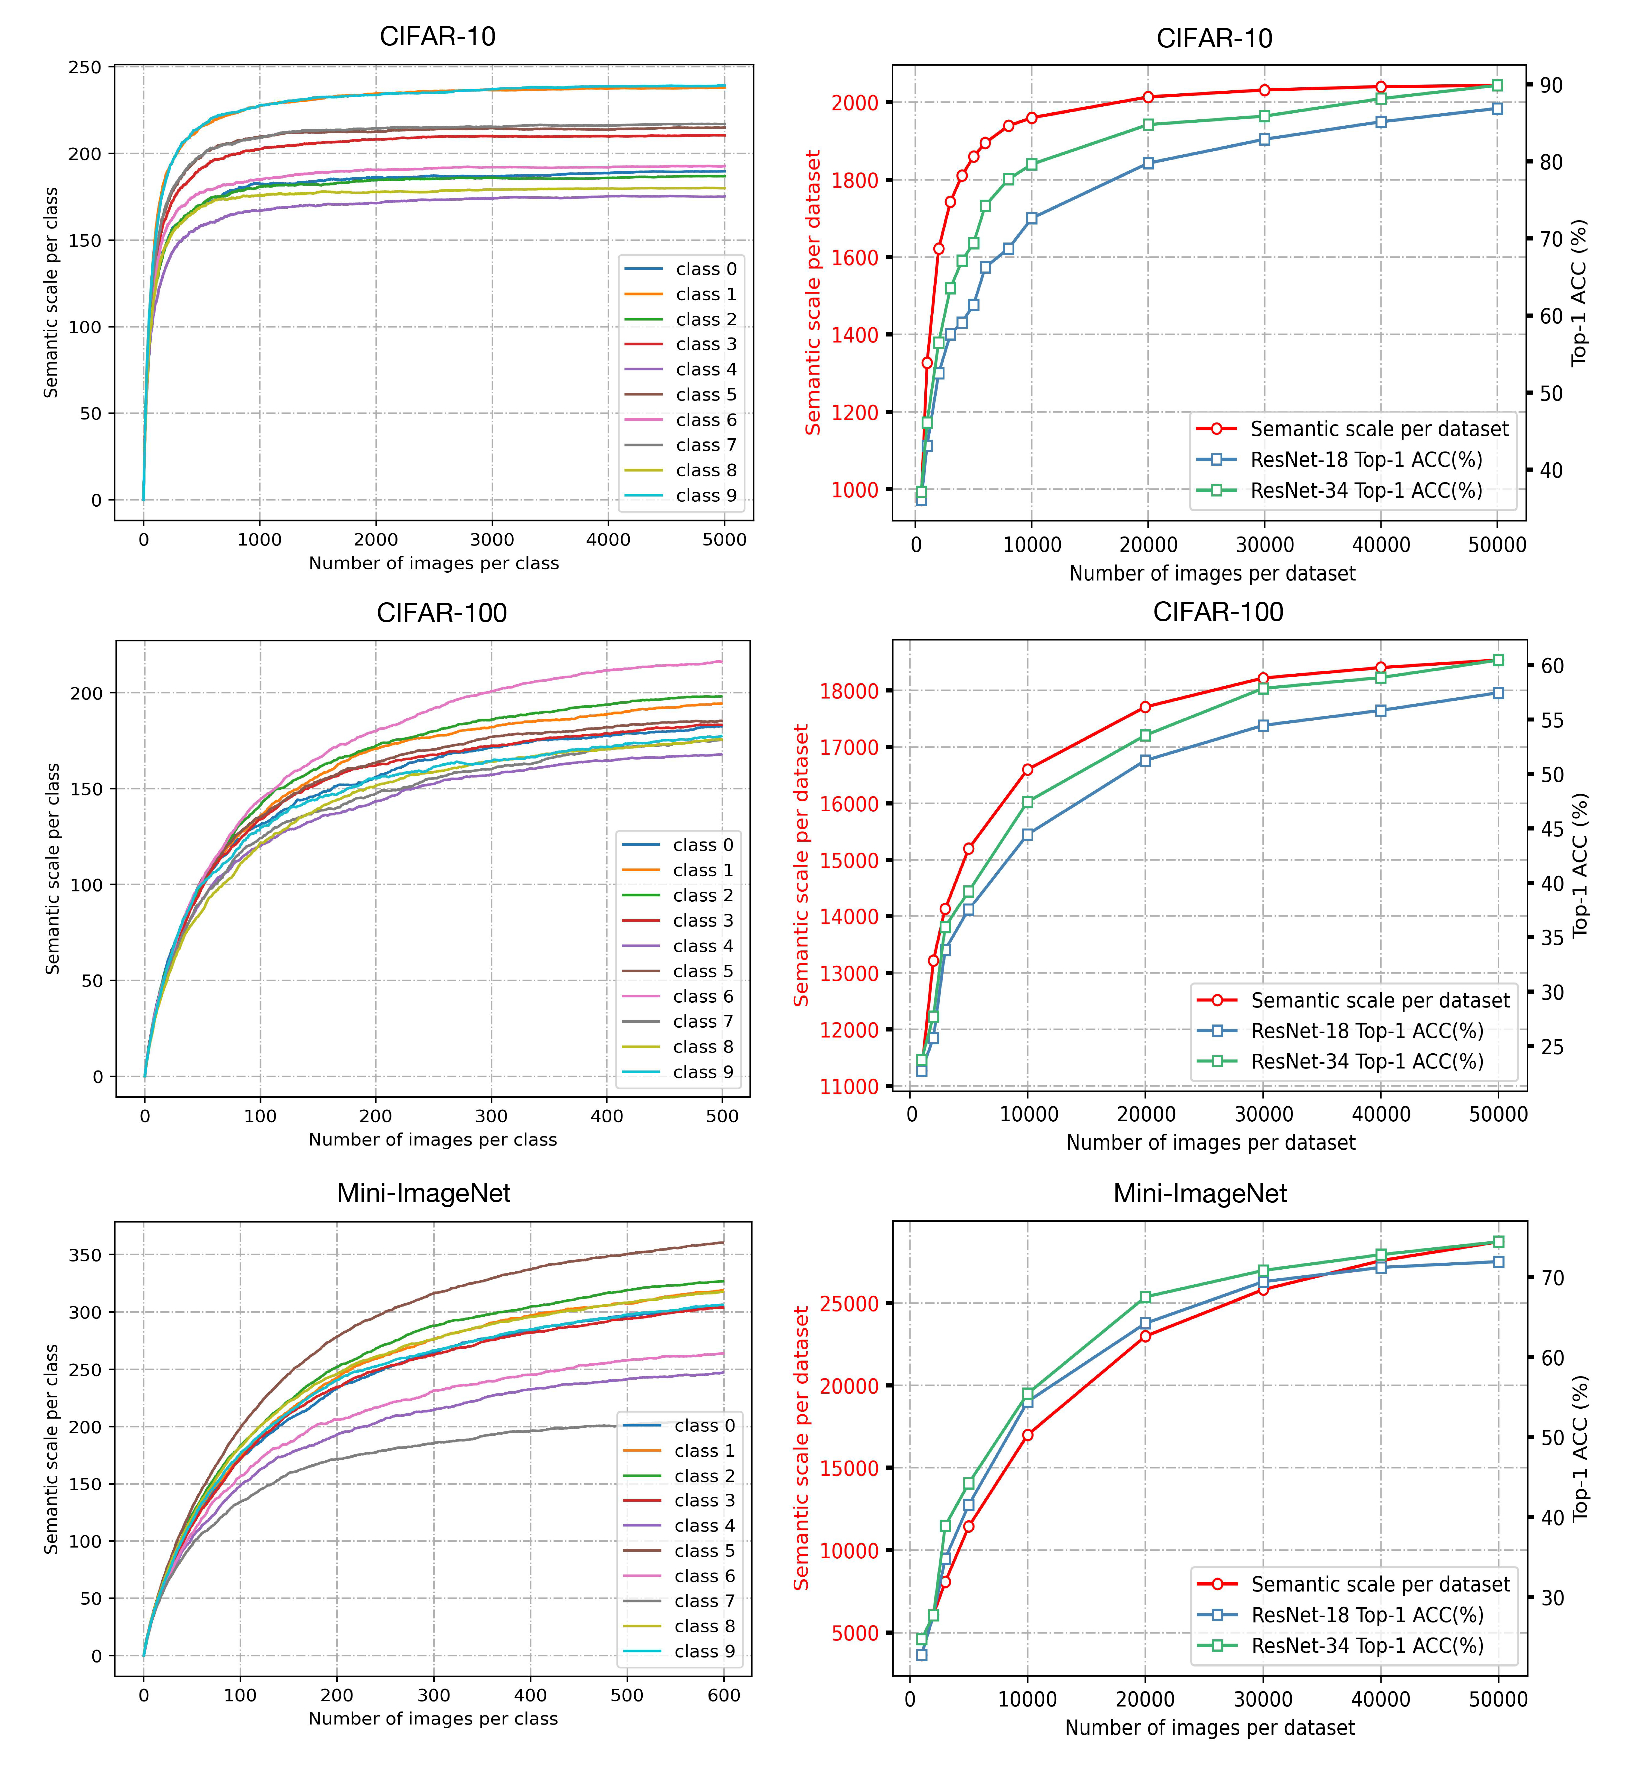
\includegraphics[width=1\columnwidth]{figure2}
\vskip -0.14in
\caption{\textbf{Left column}: curves of semantic scales with increasing number of samples for the first ten classes from different datasets. \textbf{Right column}: for different sub-datasets, curves of the sum of semantic scales for all classes and top-1 accuracy curves of trained ResNet-18 and ResNet-34. All models are trained using the Adam optimizer \cite {paper33} with an initial learning rate of $0.01$ and then decayed by $0.98$ at each epoch.}
\label{fig26}
\end{center}
\vskip -0.1in
\end{figure*}

\fi

\section{More explanation of Figure \ref{fig2}\label{K}}

To see it more clearly, we zoomed in on Figure \ref{fig2} and plotted it in Figure \ref{fig26}. Previous studies have observed that (1) given sufficient data, the classification performance gain is marginal with additional samples. (2) When the data is insufficient, the classification performance drops sharply as the number of training samples decreases. We speculate that phenomenon $1$ may be caused by the marginal effect of feature diversity. It should be noted that CB loss considers marginal effects, but it only qualitatively describes the gradual flattening of feature diversity with the increasing number of samples. Taking CIFAR-10 as an example, we first select a few samples for each class, train the model and test the accuracy. Then new samples are continuously added to the original samples instead of re-selecting more samples to train the model. The experiments corresponding to each point in Figure \ref{fig2} are trained from scratch. While increasing the data we find that there are marginal effects of semantic scale, which indicates that our proposed measurement is as expected. The marginal effects of feature diversity explain phenomenon $1$. 

However, phenomenon $2$ is not explained by the marginal effects, and the effective number of samples from CB loss does not predict phenomenon $2$ at all, because the effective number of samples does not grow faster than the number of samples (which we have analyzed in Section \ref{2}). We experimentally find that when the samples are few, the feature diversity measured by the semantic scale increases rapidly with the number of samples, and this increase is faster than the linear increase. The rapid increase of feature diversity measured by the semantic scale explains phenomenon $2$.
%-------------------------------------------------------------------------

\begin{figure*}[h]% 纵向8行,图片靠右,宽度12.5em
\begin{center}
\vskip -0.05in
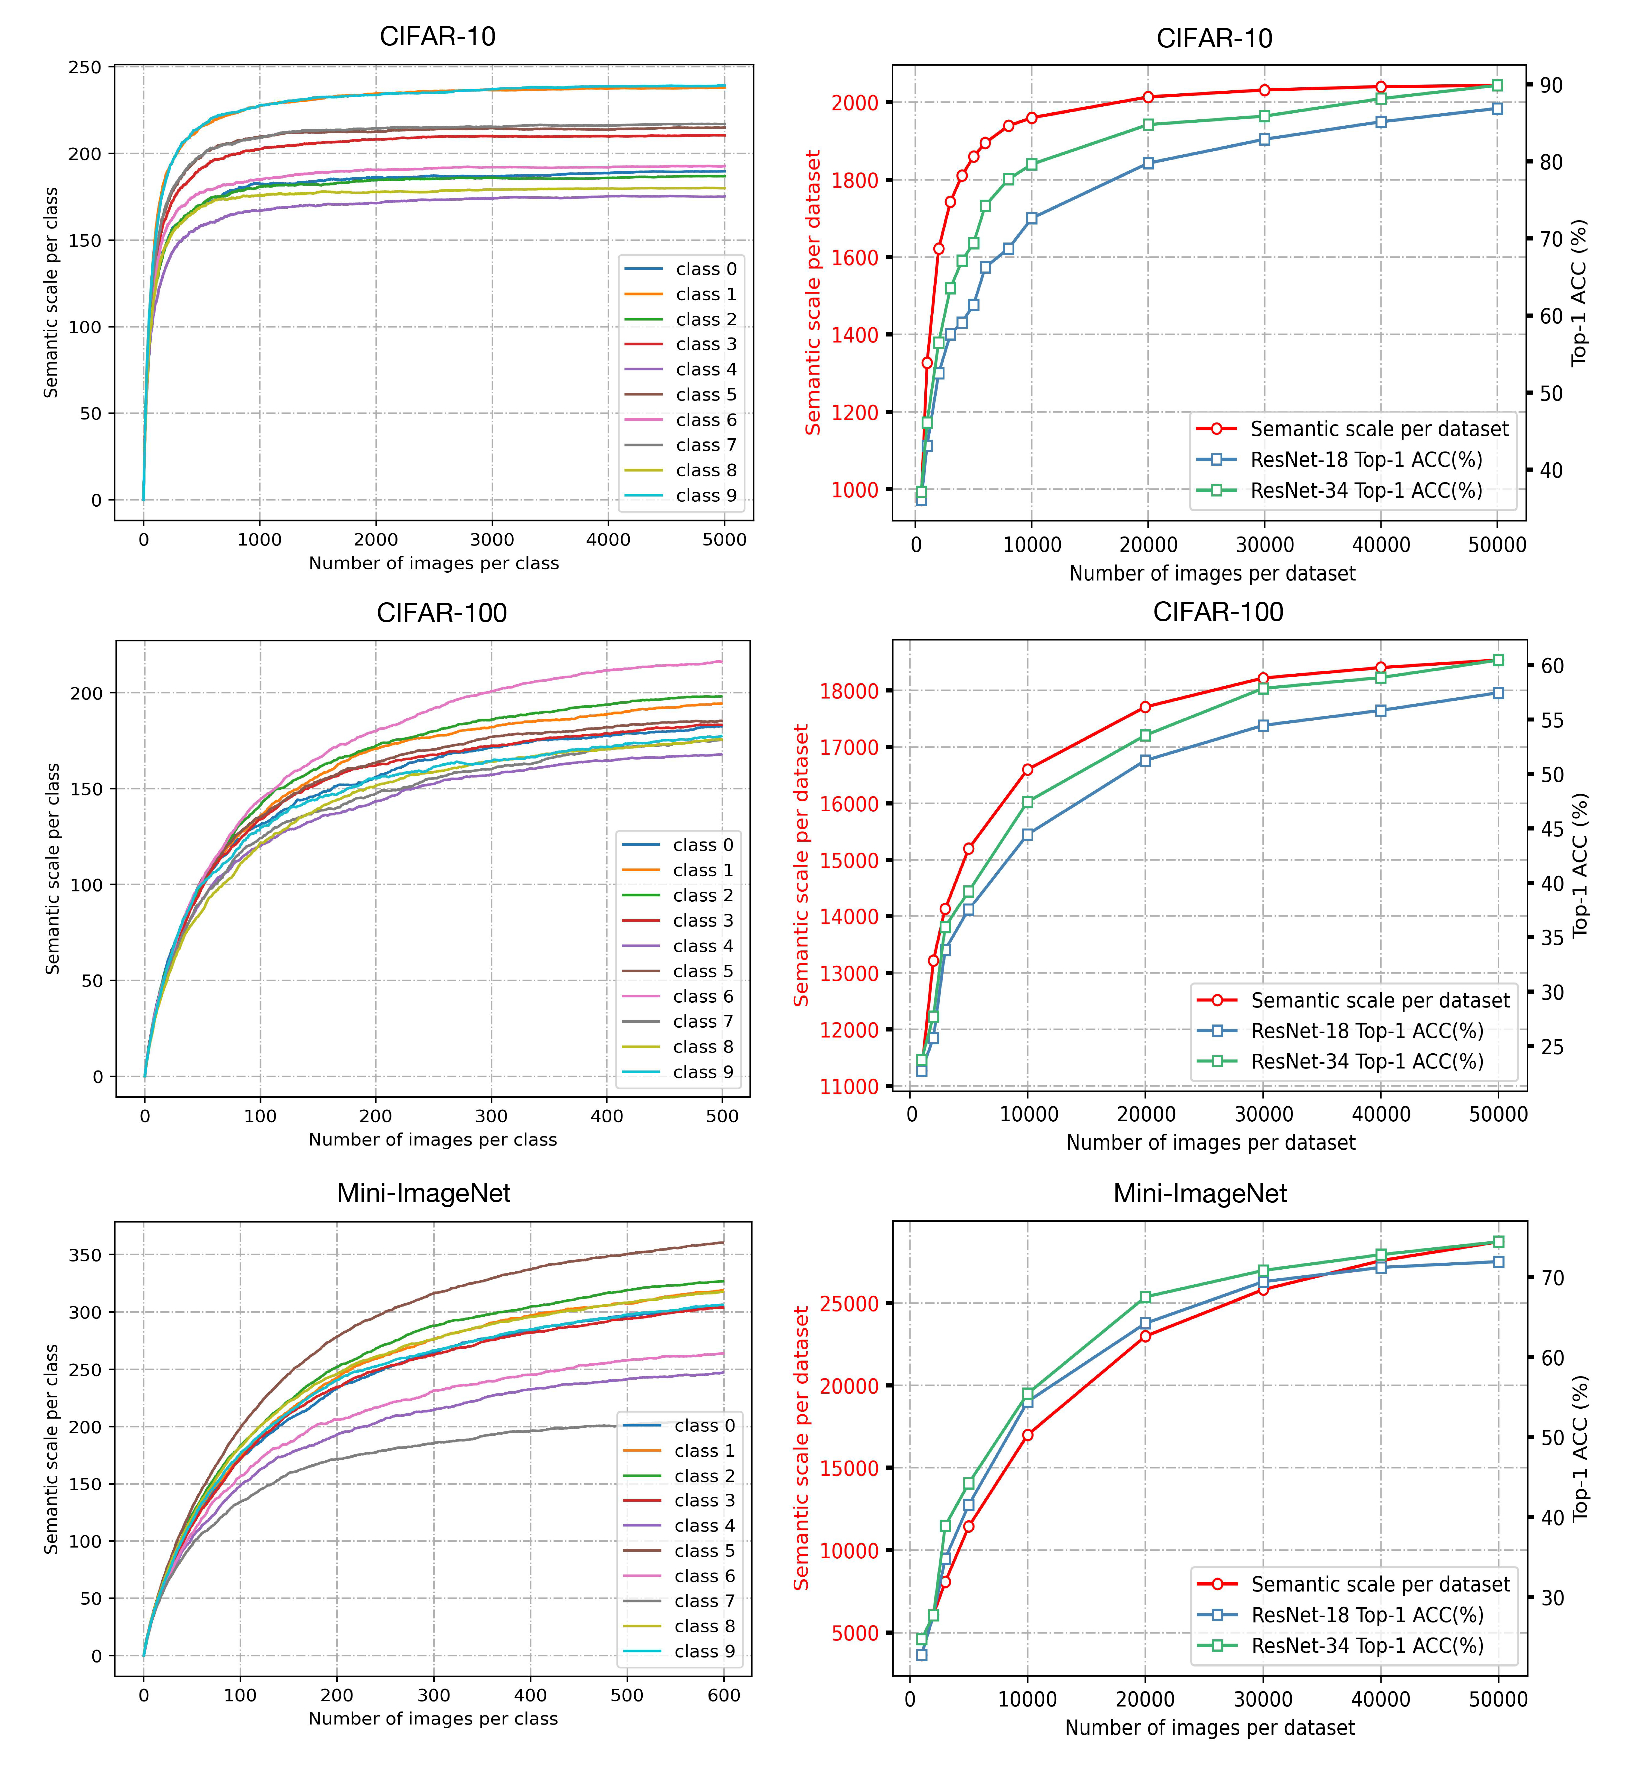
\includegraphics[width=1\columnwidth]{figure2}
\vskip -0.15in
\caption{\textbf{Left column}: curves of semantic scales with increasing number of samples for the first ten classes from different datasets. \textbf{Right column}: for different sub-datasets, curves of the sum of semantic scales for all classes and top-1 accuracy curves of trained ResNet-18 and ResNet-34. All models are trained using the Adam optimizer \cite {paper33} with an initial learning rate of $0.01$ and then decayed by $0.98$ at each epoch.}
\label{fig26}
\end{center}
\vskip -0.3in
\end{figure*}

\section{Can the semantic scale capture the hierarchical structure?\label{L}}

HCSC \cite{paper118} constructs the hierarchical structure of classes by bottom-up k-means, and we use the example shown by HCSC to validate our approach. Given the following seven classes: Poodles, Samoyeds, Labradors, Persian, Siamese, Chimpanzee, and Gorilla, each class contains $1,000$ samples, and the hierarchical structure of the seven classes is shown in Figure \ref{fig27}.

\begin{figure*}[h]% 纵向8行,图片靠右,宽度12.5em
\begin{center}
%\vskip -0.32in
\includegraphics[width=0.65\columnwidth]{fig25}
\vskip -0.05in
\caption{Image datasets typically contain multiple semantic hierarchies.}
\label{fig27}
\end{center}
\vskip -0.14in
\end{figure*}


\begin{table}[h]
%\vskip -0.15in
\renewcommand\arraystretch{1.6}
\setlength{\tabcolsep}{5pt} %修改行距
\caption{\textbf{Results of matching parent class for each child class}, where the Ratio of semantic scales denotes the ratio of the semantic scales of the parent class after mixing to before mixing, Predicted parent class means the parent class we matched for the child class, and Real parent class denotes the real parent class corresponding to the child class.}
\label{table12}
\vskip 0.1in
\centering   
\begin{scriptsize}
\begin{tabular}{|l|ccc|ccc|ccc|ccc|ccc|ccc|ccc|}
\hline \toprule 
\multicolumn{1}{c|}{child class}                                   & \multicolumn{3}{c|}{Poodles}                                    & \multicolumn{3}{c|}{Samoyeds}                                   & \multicolumn{3}{c|}{Labradors}                                  & \multicolumn{3}{c}{Persian}                                    \\ \hline
\multicolumn{1}{c|}{parent class}                                  & \multicolumn{1}{c|}{Dogs} & \multicolumn{1}{c|}{Cats} & Monkeys & \multicolumn{1}{c|}{Dogs} & \multicolumn{1}{c|}{Cats} & Monkeys & \multicolumn{1}{c|}{Dogs} & \multicolumn{1}{c|}{Cats} & Monkeys & \multicolumn{1}{c|}{Dogs} & \multicolumn{1}{c|}{Cats} & \multicolumn{1}{c}{Monkeys} \\ \hline
\multicolumn{1}{c|}{Ratio of semantic scales} & \multicolumn{1}{c|}{1.06} & \multicolumn{1}{c|}{1.72} & 1.94    & \multicolumn{1}{c|}{1.03} & \multicolumn{1}{c|}{1.68} & 1.89    & \multicolumn{1}{c|}{1.05} & \multicolumn{1}{c|}{1.64} & 1.83    & \multicolumn{1}{c|}{1.75} & \multicolumn{1}{c|}{1.08} & \multicolumn{1}{c}{1.87}    \\ \hline
\multicolumn{1}{c|}{Predicted parent class}                        & \multicolumn{1}{c|}{\Checkmark}     & \multicolumn{1}{c|}{}     &         & \multicolumn{1}{c|}{\Checkmark}     & \multicolumn{1}{c|}{}     &         & \multicolumn{1}{c|}{\Checkmark}     & \multicolumn{1}{c|}{}     &         & \multicolumn{1}{c|}{}     & \multicolumn{1}{c|}{\Checkmark}     & \multicolumn{1}{c}{}        \\ \hline
\multicolumn{1}{c|}{Real parent class}        & \multicolumn{1}{c|}{\Checkmark}     & \multicolumn{1}{c|}{}     &         & \multicolumn{1}{c|}{\Checkmark}     & \multicolumn{1}{c|}{}     &         & \multicolumn{1}{c|}{\Checkmark}     & \multicolumn{1}{c|}{}     &         & \multicolumn{1}{c|}{}     & \multicolumn{1}{c|}{\Checkmark}     &\multicolumn{1}{c}{}         \\ 
\bottomrule \hline
\end{tabular}

\setlength{\tabcolsep}{9.7pt} %修改行距
\begin{tabular}{l|ccc|ccc|ccc}
\hline \toprule 
\multicolumn{1}{c|}{child class}                                   & \multicolumn{3}{c|}{Siamese}                                    & \multicolumn{3}{c|}{Chimpanzee}                                 & \multicolumn{3}{c}{Gorilla}                                     \\ \hline
\multicolumn{1}{c|}{parent class}                                  & \multicolumn{1}{c|}{Dogs} & \multicolumn{1}{c|}{Cats} & Monkeys & \multicolumn{1}{c|}{Dogs} & \multicolumn{1}{c|}{Cats} & Monkeys & \multicolumn{1}{c|}{Dogs} & \multicolumn{1}{c|}{Cats} & Monkeys \\ \hline
\multicolumn{1}{c|}{Ratio of semantic scales} & \multicolumn{1}{c|}{1.69} & \multicolumn{1}{c|}{1.02} & 1.84    & \multicolumn{1}{c|}{1.87} & \multicolumn{1}{c|}{1.83} & 1.06    & \multicolumn{1}{c|}{1.82} & \multicolumn{1}{c|}{1.89} & 1.02    \\ \hline
\multicolumn{1}{c|}{Predicted parent class}                        & \multicolumn{1}{c|}{}     & \multicolumn{1}{c|}{\Checkmark}     &         & \multicolumn{1}{c|}{}     & \multicolumn{1}{c|}{}     &\Checkmark         & \multicolumn{1}{c|}{}     & \multicolumn{1}{c|}{}     &\Checkmark         \\ \hline
\multicolumn{1}{c|}{Real parent class}        & \multicolumn{1}{c|}{}     & \multicolumn{1}{c|}{\Checkmark}     &         & \multicolumn{1}{c|}{}     & \multicolumn{1}{c|}{}     &\Checkmark         & \multicolumn{1}{c|}{}     & \multicolumn{1}{c|}{}     &\Checkmark         \\ 
\bottomrule \hline
\end{tabular}
\end{scriptsize}
\vskip -0.1in
\end{table}

We collect $1,000$ images for each of the three parent classes (Dogs, Cats, and Monkeys), which can adequately represent the three parent classes, i.e., the feature richness is sufficient. \textbf{Then can the semantic scale be used to match the correct parent classes for the seven classes?} According to our theory, the manifolds of the child classes should be in the manifold of the corresponding parent class, and they have an inclusion relationship. Therefore, when the data of the child classes are mixed into the data of the parent class, the manifold volume of the parent class will not change significantly. We propose the matching method of semantic hierarchy based on this property. The specific steps are as follows.

\begin{itemize}
     \item[(1)] train a ResNet-18 classification model on seven child classes. We set the batch size to $64$ and adopt the adam optimizer with a learning rate of $0.01$ (linear decay), a momentum of $0.9$, and a weight decay factor of $0.005$.
     \item[(2)] Extract the features of all samples from seven child classes and three parent classes.
     \item[(3)] Calculate the semantic scales of the three parent classes.
     \item[(4)] Select a child class $c$ from the seven child classes.
     \item[(5)] Mix the data of child class $c$ into the data of each parent class and calculate the semantic scale of the mixed data, we can get three values.
     \item[(6)] Calculate the changes in the semantic scales of the three parent classes and sort them.
     \item[(7)] Match the parent class with the smallest change in semantic scale for child class $c$.
     \item[(8)] Perform steps (3) to (7) for the remaining six child classes.
\end{itemize}

We summarize the ratio of the semantic scales of the parent classes after mixing to before mixing in Table \ref{table12}. If the change in the semantic scale of a parent class is small after a child class is mixed into that parent class, they are considered to have a nested relationship. Based on the above method, we successfully match each child class to the parent class. Experimental results show that our proposed measure of semantic scales can capture the semantic hierarchy of classes. Our study can inspire hierarchical feature learning as well as facilitate its performance in downstream tasks.

\section{Future Work and Challenges\label{J}}

\subsection{Model-Independent Measure of Data Difficulty\label{J.1}}

The performance of the models varies across classes. In the past, it was believed that model bias was caused by an imbalance in sample numbers, but a growing body of research suggests that sample numbers are not the only factor affecting model bias. Of course, model bias is also introduced not by the model structure, but by the characteristics of the data itself that affect model performance. Therefore, it is very important to propose model-independent measurements to represent the data itself, and this work will greatly contribute to our understanding of deep neural networks. In this paper, the effect of the volume of the data manifold on the model bias is explored from a geometric perspective. It provides a new direction for future work, namely the geometric analysis of deep neural networks. The geometric characteristics of the data manifold will help us further reveal how neural networks learn and inspire the design of neural network structures.

\begin{figure*}[h]% 纵向8行,图片靠右,宽度12.5em
\begin{center}
\vskip -0.05in
\includegraphics[width=1\columnwidth]{fig24}
\vskip -0.1in
\caption{Changes in the geometry of data manifolds as they are transformed in a deep neural network. The classification process of the data includes untangling the manifolds from each other and separating the different manifolds.}
\label{fig25}
\end{center}
\vskip -0.1in
\end{figure*}

\subsection{A Geometric Perspective on Data Classification\label{J.2}}

Natural datasets have intrinsic patterns that can be generalized to the manifold distribution principle: the distribution of a class of data is close to a low-dimensional manifold. As shown in Figure \ref{fig25}, data classification can be regarded as the unwinding and separation of manifolds. When a data manifold is entangled with other perceptual manifolds, the difficulty of classifying that manifold increases. Typically, a deep neural network consists of a feature extractor and a classifier. Feature learning can be considered as manifold unwinding, and a well-learned feature extractor is often able to unwind multiple manifolds for the classifier to decode. In this view, all factors about the manifold complexity may affect the model's classification performance. Therefore, we suggest that future work can explore the inter-class long-tailed problem from a geometric perspective.


\subsection{Introduce Semantic Scale Imbalance in Object Detection\label{J.3}}

Long-tailed distribution is one of the main difficulties faced by object detection algorithms in real-world scenarios. The classical object detection algorithms are generally trained on some manually designed datasets with relatively balanced data distribution. In contrast, the accuracy of these algorithms tends to suffer significantly on long-tailed distributed datasets. So far, methods for foreground-background imbalance and class imbalance have been proposed extensively, but these methods are based on the number of objects to define the degree of imbalance and cannot explain more phenomena. We will give examples below.

In the field of object detection, it is often encountered that although a class does not appear frequently, the model can always detect such instances efficiently. It is easy to observe that classes with simple patterns are usually easier to learn, even if the frequency of such classes is low. Therefore, classes with low frequency in object detection are not necessarily always harder to learn. We believe that it is a valuable research direction to analyze the richness of the instances contained in each class, and then pay more attention to the hard classes. The dimensionality of all images or feature embeddings in the image classification task is the same, which facilitates the application of the semantic scale proposed in this paper. However, the non-fixed dimensionality of each instance in the field of object detection brings new challenges, so we have to consider the effect of dimensionality on the semantic scale, which is a direction worthy of further study.

\subsection{Challenges of class imbalance in deep learning\label{J.4}}

Class imbalance remains a major challenge in the field of deep learning. Data imbalance classification, although widely studied, still lacks effective and clear methods and guidelines. The problem of object detection for class imbalance is still in its infancy and requires a greater investment of attention. In the following, we summarize the important future challenges and research directions in this field.

\begin{itemize}
     \item[(1)] \emph{The more precise measure of class difficulty}. An increasing number of studies have shown that the sample number does not accurately reflect the accuracy of the model in recognizing classes. Therefore, more extensive measures should be proposed to redefine the long-tail distribution to facilitate classification and object detection tasks and further expand the scope of research on long-tailed recognition. For example, a dataset with perfectly balanced sample numbers may not be balanced under other measures.

\begin{figure*}[h]% 纵向8行,图片靠右,宽度12.5em
\begin{center}
\vskip -0.14in
\includegraphics[width=0.95\columnwidth]{nfig35}
\vskip -0.2in
\caption{Class-level long-tailed distribution and intra-class attribute long-tailed distribution.}
\label{fig26}
\end{center}
\vskip -0.15in
\end{figure*}

     \item[(2)] \emph{Long-tailed distribution of properties in classes}. As shown in Figure \ref{fig26} \cite{paper115}, previous studies have focused on the imbalance between classes and ignored the imbalance of properties within each class. For example, most pandas have black and white fur, and only a small proportion of pandas are brown. In visual recognition tasks, we should not only pursue the overall accuracy of the class but also pay attention to whether samples with sparse properties in a class can be classified accurately. In medical image classification, the above point is particularly important. For example, pulmonary diseases contain many different types of diseases, and generally the more severe the disease tends to have a smaller sample number, suggesting that there is an imbalance of properties under the label of pulmonary disease. We hope to be able to recognize more severe diseases more accurately so that patients do not miss the best time to treat them.

     \item[(3)] \emph{Generalization performance of the model outside the training domain of the tail class}. As shown in Figure \ref{fig27}, tail classes often have very few samples, so these samples do not well represent the true distribution of the tail classes, which results in the model consistently failing to learn and adapt to the tail classes correctly. Obviously, recovering the underlying distribution of the tail classes helps the generalization performance of the model outside the training domain of the tail classes. It is currently shown that similar classes have similar distribution statistics (variance), which can lead researchers to recover the underlying distribution of tail classes. However, the current research is still in its infancy, and it is not a sufficiently stringent assumption that similar classes have similar variances. Therefore, we hope that in the future researchers will be able to help recover the true distribution of tail classes by more means.

\begin{figure*}[h]% 纵向8行,图片靠右,宽度12.5em
\begin{center}
%\vskip -0.08in
\includegraphics[width=1\columnwidth]{fig1a}
\vskip -0.05in
\caption{(a) When the samples uniformly cover the true data distribution, the model can learn the correct decision boundaries and can correctly classify unfamiliar samples to be tested. (b) When the samples cover only a portion of the true distribution, unfamiliar samples to be tested are highly likely to be misclassified due to the error in the decision boundary. (c) The direction in which the arrow points is the best direction to expand the sample.}
\label{fig27}
\end{center}
\vskip -0.13in
\end{figure*}

     \item[(4)] \emph{How to choose the appropriate long-tailed recognition method in the task}. Up to now, a large number of visual recognition methods on long-tail distribution have been proposed. While individual methods have positive performance in long-tailed recognition tasks, some combinations of methods may have negative effects. Few studies have focused on the selection and combination of different training techniques and methods. In the future, it is possible to explore how to select existing methods on specific tasks, and further, effective combinations of different methods are important. 
     \item[(5)] \emph{Multi-domain deep long-tailed learning}. Past research has typically focused on the problem of long-tailed distribution over a single domain, which has limited the research ideas. As shown in Figure \ref{fig28}, data from multiple domains can complement each other to alleviate the long-tailed distribution of classes \cite{paper119}. For example, in plant and animal classification, cameras are placed in different places to capture animals, but some animals only appear in a fixed area, which leads to different label distributions for animals captured by different cameras. But by combining the data from all cameras, a more balanced class can be obtained. Similarly, a similar situation occurs in other practical applications. For example, in a visual recognition problem, the few classes from "photo" images can be complemented by a potentially rich sample from "sketch" images. In autonomous driving, a few classes of "real" life accidents can be enriched by accidents generated in "simulations". In addition, in medical diagnosis, data from different populations can be mutually augmented, e.g., a small sample from one institution can be combined with the majority of possible instances from other institutions. In these examples, different data types can act as different domains, and such multi-domain data can also be utilized effectively to address data imbalances.

\begin{figure*}[h]% 纵向8行,图片靠右,宽度12.5em
\begin{center}
%\vskip -0.14in
\includegraphics[width=1\columnwidth]{fig36}
\vskip -0.15in
\caption{The frequency of the same class appearing in different domains may differ significantly, assuming a smaller sample of horses in the real world and a larger number of horses in cartoon form. Images from different domains can complement each other to form a dataset with a balanced sample number. The purpose of multi-domain deep long-tailed learning is to train unbiased models using data from multiple domains and generalize over all domains.}
\label{fig28}
\end{center}
\vskip -0.12in
\end{figure*}

     \item[(6)] \emph{Recognition of unbalanced data streams}. Continuous learning aims to process new data that is continuously generated in order to dynamically update and adapt the model to the latest data domain. Challengingly, as new data is generated, the degree of imbalance between classes changes and what used to be a tail class may become a head class. The long-tailed distribution of properties within classes can also affect the performance of the model if concept drift occurs. Thus the key to handling unbalanced data streams is to evaluate the class-level difficulty and the long-tailed distribution of properties within classes in real time, which is a huge challenge. 
     \item[(7)] \emph{Augmentation methods for other modally unbalanced data}. Methods for multi-sample synthesis are widely used in image data augmentation, such as Mixup and Cutout, but there is still a lack of data augmentation methods for other modal data (e.g., speech and table). Researchers can design a more general method to generate samples of any type of data.
     \item[(8)] \emph{Other long-tailed visual recognition tasks}. Current research focuses on long-tail image classification, while less attention has been paid to long-tail object detection, image segmentation, and regression tasks. In object detection, there are multiple imbalances, such as foreground-background imbalance and imbalance between classes belonging to the foreground, which are unresolved challenges. With further applications of deep learning, research on imbalance learning in various fields will be of great benefit for real-world applications.
\end{itemize}

This study suggests some future avenues of inquiry to further deepen and expand the study of unbalanced learning. Of course, the scope of future inquiry into unbalanced learning is not limited to the eight challenges mentioned above, and we believe that new questions will arise in the course of inquiry into these eight challenges, but that researchers will eventually address them over time.

\epigraph{\emph{In everything balance has to be gained. Through balance you will come nearer to truth, because truth is the ultimate balance}.}{Osho}

\iffalse
\newpage

\hypersetup{hidelinks} 
\tableofcontents
\listoffigures
\listoftables

\fi





\iffalse
A \gls{np} estimates a stochastic process implicitly defined with neural networks given a stream of data, rather than pre-specifying priors already known, such as Gaussian processes. An ideal \gls{np} would learn everything from data without any inductive biases, but in practice, we often restrict the class of stochastic processes for the ease of estimation. One such restriction is the use of a finite-dimensional latent variable accounting for the uncertainty in the functions drawn from \glspl{np}. Some recent works show that this can be improved with more ``data-driven’’ source of uncertainty such as bootstrapping. In this work, we take a different approach based on the martingale posterior, a recently developed alternative to Bayesian inference. For the martingale posterior, instead of specifying prior-likelihood pairs, a predictive distribution for future data is specified. Under specific conditions on the predictive distribution, it can be shown that the uncertainty in the generated future data actually corresponds to the uncertainty of the implicitly defined Bayesian posteriors. Based on this result, instead of assuming any form of the latent variables, we equip a \gls{np} with a predictive distribution implicitly defined with neural networks and use the corresponding martingale posteriors as the source of uncertainty. The resulting model, which we name as \gls{mpnp}, is demonstrated to outperform baselines on various tasks.


\section{Introduction}
\label{intro}

% very general intro on ML
Machine Learning (ML) gained a huge success in the last decades, becoming one of the most popular and studied branches of artificial intelligence \cite{jordan2015machine}. ML methods are widely used in many fields of research, with the aim of obtaining a general working learning rule from input data, namely a prediction function, to be used for future predictions of never-seen-before data.
Specifically, ML algorithms have been widely exploited in industrial processes, playing a relevant role in a wide range of applications: Industry 4.0 \cite{angelopoulos2019tacklin}, healthcare \cite{kourou2015machine}, transportation \cite{hamner2010predicting}, natural science \cite{yao2008quantitative}, social media \cite{balaji2021machine}, fraud detection \cite{awoyemi2017credit} and so on.

% General intro on AD
Anomaly detection represents an important and widely used ML task, broadly applied in various domains and applications where the issue of monitoring unexpected data behaviour is essential. This task defines the process of identifying anomalous data, i.e., data being characterised by a different behaviour with respect to other data distinguishing itself from the rest of the dataset. To date, there is no unanimously accepted definition but broadly speaking, an anomalous point, often named equivalently anomaly or outlier, is defined \textit{as an observation that deviates so much from other observations as to arouse suspicion that it was generated by a different mechanism} \cite{hawkins1980identification}. Anomaly detection is commonly tackled in many industrial scenarios, such as credit card fraud detection \cite{ghosh1994credit}, insurance fraud detection \cite{fawcett1999activity}, insider trading detection \cite{donoho2004early}, medical anomaly detection \cite{wong2003bayesian}. In these dynamic and often complex contexts, the problem of detecting anomalies is crucial in order to predict and avoid failures as well as to perform fault detection. In many industrial processes in fact, data-driven approaches for smart monitoring (for example predictive maintenance) have a key role, allowing to identify and isolate faults and to prevent future sudden failures. To solve this problem, anomaly detection represents an efficient solution.
Generally, in this scenario a great amount of collected data are available but, since labelling is an expensive and time consuming process, there is a lack of ground truth labels, undoubtedly stating whether or not a point is anomalous. The learning problem therefore is unsupervised and the algorithm can just blindly look at the structure of the dataset, without a clear definition of what is an anomaly from the user perspective. Therefore unsupervised algorithms can only detect samples that exhibit some general property different to the rest of the dataset, for example some approaches look for points far from the majority, or detect points living in low density areas.

% Anomalies are domain specific
Unfortunately, anomalies are strongly domain specific \cite{foorthuis2021nature}: as stated above, since no official definition is given, the concept of what an anomaly is entirely relies on the application in question. Specifically, it may happen that a set of data has different anomalies based on the given application domain and that the same data may be considered anomalous in one domain but normal in another \cite{sejr2021explainable}. For instance looking at data acquired by a measuring instrument, the manufacturer might define anomalies as events where the instrument has a faulty behaviour while the end-user might be more interested in events where the measured process behaves in a previously unseen way \cite{barbariol2020self}. As a direct consequence, training a domain specific anomaly detector would require a full set of labeled data to capture the user definition of anomaly. 

% full set of labels are too expensive
In real world applications, assigning labels to input data pose a considerable challenge to take into account \cite{zhu2009introduction}. In order to train reliable models, a large amount of labeled data is needed but, in practical scenarios, labeled examples are limited or often too expensive and time-consuming to collect, leading to a huge issue to face. Obtaining labels requires an often too expensive cost to take care of since the labeling procedure is usually carried on by a human domain expert who manually labels each point with a time-consuming and demanding routine. Moreover, by definition anomalous points are rare and difficult to spot, making the problem a difficult challenge to be solved. 
%as well as extremely unbalanced one. 
%\gas{Forse toglierei la roba dell'unbalanced qua o lo scriverei diversamente} 

% unsupervised AD is used in practice, but has no precise anomaly definition
Due to the difficulty of finding labeled points, in practical contexts anomaly detection is often treated as an unsupervised learning task. For the classical unsupervised anomaly detection problem, the purpose is to detect outliers with no use of labeled data based on the fact that normal data greatly outnumbers anomalous data, and anomalies are very different with respect to inliers. Unsupervised anomaly detection models are not tuned for the precise domain of application but are generally based on identifying rules based on specific data characteristics, such as density based algorithms, distance based methods etc. \cite{hochenbaum2017automatic, hill2010anomaly, knorr1998algorithms, breunig2000lof}. 
However recent literature \cite{das2016incorporating,sejr2021explainable} distinguishes the outliers to the anomalies: the first are the points highlighted by an unsupervised model, while the second are the ones the user actually sees as anomalous. As the unsupervised model is not directly tuned to the detection of the anomalies, the outliers might weakly correlate with them. 

% outliers do not coincide with anomalies
Therefore, running unsupervised anomaly detection algorithms may be risky and often misleading: as stated above anomalies are strongly domain dependent and as a direct consequence, an unsupervised detector might not identify anomalous data which should be considered as such, as well as could wrongly detect as anomalies points which are normal based on the context taken under consideration \cite{das2016incorporating}. Figure \ref{anomalyvsoutlier} presents a visual representation of the strong connection between anomalous data points and context domain. Specifically, the plot shows the two-dimensional projection of the \textit{vowels} dataset \cite{Rayana}. As it can be seen, anomalies are not defined just as data points lying far or in low-density regions, but they form a class with a specific pattern defined by domain-experts, making complicated for the automatic detector to correctly identify them.

\begin{figure}
    \centering
    \includegraphics[scale=0.6]{vowelsPCA.pdf}
    \caption{Projection of the \emph{vowels} dataset on 2 dimensions using Principal Component Analysis. Purple data points are normal data, yellow points are anomalous data. Two aspects are clearly visible: i) it is impossible to separate anomalies from normal data with only two features and ii) anomalies tend to form a different class and might be quite different from general outliers. Not all the data points lying in low density areas or far from the majority are defined as anomalies, but just the ones lying in a specific part of the space. 
    %As shown, anomalies do not tend to have any peculiar discrepancies with respect to normal points. On the contrary, they lie on the same portion of space occupied by normal points.
   As a consequence, in the considered scenario, identifying anomalies might be a challenging task for an unsupervised detector.}
    \label{anomalyvsoutlier}
\end{figure}


% presentazione di IF
Among the unsupervised models, a very popular anomaly detection algorithm is the Isolation Forest (IF) \cite{liu2008isolation, liu2012isolation}, which presents a very different approach w.r.t. the majority of models: instead of creating a profile for normal data, it explicitly tries to isolate anomalies. To do it, IF relies on two assumptions: anomalies are fewer in number and they have very different attributes compared to normal data. 


%\gas{Manca imho il discorso: AD pervasiva -> ci sono i sistemi di supporto alle decisioni -> abbiamo ora la possibilità in tante applicazioni di ottenere una taggatura non costosa dopo aver sviluppato un primo sistema di Anomaly Detection}

In Decision Support Systems (DSS) \cite{keen1980decision}, data streams are analysed in order to quickly extract strategic decisions on complex problems. Such process is monitored by users who frequently interact with the system and represent the actual decision maker of the whole process. In such framework, \approach represents an extremely appealing approach. Specifically, if a DSS is present, as a direct consequence, a user is already overseeing the process and inspecting data points: considering an unsupervised anomaly detection problem, inexpensive labels may be obtained in a fast way and using \approach the model may be inexpensively updated. 


% novelty
In this paper we describe a procedure able to tune the detector model on domain specific anomalies by interacting with a human expert. To perform the proposed tuning method, not every training data are presented and labeled but a subset is automatically selected so that the number of interactions between the system and the human is minimised. The core idea is to ask labels corresponding to the most significant points to reduce the labeling cost and at the same time to maximize the detection performance. As a direct consequence, the proposed procedure may be regarded as an Active Learning (AL) based model \cite{kumar2020active}. 

\begin{figure}
\centering
\usetikzlibrary{automata, arrows.meta, positioning}
 \begin{tikzpicture} [node distance = 4cm, on grid, auto]
 
\node (q0) [draw,lightgray, rounded corners, text width=1.5cm,yshift=-1.2cm, align =center] {\textcolor{black}{unlabeled \\dataset}};
\node (q1) [draw,lightgray, text width=1.5cm, rounded corners,above right = of q0,  yshift=-1.2cm,align =center] {\textcolor{black}{active \\selection}};
\node (q2) [draw,lightgray,rounded corners, text width=1.5cm, below right = of q1,yshift=1.2cm,align =center] {\textcolor{black}{labeled \\dataset}};
\node (q3) [draw,lightgray,rounded corners, text width=1.5cm, below left = of q2,yshift=1.2cm,align =center] {\textcolor{black}{learning \\model}};
 
\path [-stealth, thick]
    (q0) edge [lightgray, bend left]  (q1)
    (q1) edge [lightgray,bend left]  (q2)
    (q3) edge [lightgray,bend left]  (q0)
    (q2) edge [lightgray,bend left]  (q3);
\end{tikzpicture}
\caption{Active learning core structure. At each iteration a novel point is actively selected from the unlabeled set of data and the corresponding label is requested. Based on the received information, the model is modified.} \label{al}
\end{figure}

Indeed AL represents a training approach particularly suitable when labeled samples are too expensive or difficult to obtain. Specifically, AL is a particular ML algorithm based on a key idea: despite the shortage of labeled data, high accuracy results may be obtained if the training algorithm is allowed to choose the points to be labeled and learn from them \cite{settles1995active}. An AL algorithm asks an oracle to label the data considered most informative with an iterative approach. Doing so, since the queried points are directly selected by the learning algorithm, the amount of necessary labeled data is much smaller than that required for classical supervised ML approach. Figure \ref{al} shows the core structure of any AL algorithm: at each iteration the model is updated using the labelled dataset, and is allowed to ask for a new label in the unlabelled dataset. This process repeats until the model reaches sufficient performances or when the number of iterations reaches the maximum budget.

%\\In recent years, some active learning-based anomaly detection algorithms have been proposed.
%The idea of incorporating expert feedback in unsupervised anomaly detection algorithms aims at improving the achieved performance adding a relatively small computational cost. Active anomaly detection (AAD) algorithm \cite{das2016incorporating, das2017incorporating} proposes an active learning anomaly detection approach where points are ranked based on their anomalous behavior. The main goal is to maximize the number of true anomalies presented to the domain expert. An inclusion of AAD algorithm in the One Class Support Vector Machine (OCSVM) framework is tackled in \cite{lesouple2021incorporating}.
%Always using OCSVM, an expert feedback inclusion has been recently proposed %\cite{lesouple2021introduce}: to solve the problem, the paper combines together the $\mu$-SVM for the %labeled data and the OCSVM for the unlabeled set of data.

This paper focuses on the Isolation Forest detector, and suggests a strategy to tune it towards the user definition of anomaly. In this work the authors compare two AL query policies to ask the user new labels, and other two policies to update the internal structure with minimal computational effort. The goal is to increase the performance of the detector as much as possible, keeping very low both the labelling effort and the updating procedure. Moreover this method has two key advantages over the supervised and computationally expensive models: as it relies on an initial unsupervised training, it can start to work when there are no labels, but more importantly it can work even if instances from only one class are labelled. This is particularly useful when obtaining labels from the anomalous class is very uncommon or expensive.

%\gas{The rest of the papers is organized as follows: ...}
The rest of the paper is organized as follows. Initially, in Section \ref{rw} we outline the Isolation Forest in detail, and we indicate an existing active learning-based anomaly detection algorithm that will be used as a benchmark in thos work. Then, in Section \ref{pm} we illustrate the proposed model \approach: namely, we describe the strategies suggested to query the points as well as the approaches employed to update the model. In Section \ref{exp} we test \approach, comparing it with other models in relation to multiple real set of data. Finally, in Section \ref{conclusions} we draw conclusions for the present work.

%This paper compares two AL query strategies for anomaly detection using Isolation Forest. The algorithm key idea is to modify the internal structure of the unsupervised model based on a small amount of labeled data queried to the domain expert, trying to minimize the labelling effort but at the same time maximising the detection performance. Specifically, the presented model is based on the Isolation Forest model, i.e., the basic concept used to classify anomalies remains isolating data points from the rest of the dataset. Anyway, an innovative approach is used to query the labels and to update the model: novel information is achieved with the use of an active learning strategy by which the inner framework of the model is modified in order to match with the information obtained. Once the information is achieved, a user friendly iterative process allows to adapt the model by adjusting its structure on the basis of the novel input.
%The proposed method relies onto two distinguished yet essential issues: a process to select the most significant points and a tuning procedure to modify the structure of the model based on the information achieved. 
%This method has two key advantages over the supervised computationally expensive models: it is extremely computationally efficient and works even if instances from only one class are labelled.
%Based on the treated framework and on the data in hand, active learning algorithms are characterized by many possible query strategies \cite{settles1995active}. In this way, based on the considered purpose, the suitable query strategy may be selected and the corresponding most informative point may be labeled. 
%In the same way, we propose two possible approaches to address the selection of points to be labeled, producing two different query strategies with respect to both their benefits as well as their computational costs.
%\tommi{bisognerebbe scrivere che testiamo il nostro metodo su dataset reali e pubblichiamo il codice bla bla bla.}
%The importance of the algorithm...
%As we will see later the proposed model is based on...
%Section \ref{} ecc..
%list of the notation - simboli usati fare tabella





%\tommi{monitoring unexpected behaviour?} is essential. 
 %Even if, to date, there is no clear or official definition, broadly speaking, an anomalous point, also known as anomaly or outlier, is defined \textit{as an observation that deviates so much from other observations as to arouse suspicion that it was generated by a different mechanism} \cite{hawkins1980identification}. In general, an anomaly is identified as a variation from the norm, a data being characterised by a different behaviour with respect to other data that distinguishes itself from the rest of the dataset. Consequently, anomaly detection algorithms aim at detecting or identifying data that seem not to conduct themselves with a standard trend.
%\tommi{non sembra che parliamo di distribuzione gaussiana?}. 
%Anomaly detection techniques may be divided into three groups based on the available data in use: supervised, unsupervised and semi-supervised. 
%If the dataset contains labeled data, any technique for binary classification may be used, leading to highly accurate results. 
%Unfortunately, a critical challenge of anomaly detection is the lack of labeled data \cite{chandola2009anomaly}. Obtaining labels requires an often too expensive cost to take care of, since the labeling procedure is usually carried on by a human expert domain who, by hand labels each point with a time consuming and demanding routine. To solve this matter, semi-supervised or unsupervised techniques are employed. In the first scenario, a labeled portion of the original dataset is required, usually belonging to the most representative normal class, and, based on such labeled data, a model representing the normal behaviour is produced. \tommi{dici?} Generally, in fact, labeling normal data requires less efforts: normal points tend to have a common and more static behavior, making it easier to  be identified.
%For the classical unsupervised anomaly detection problem, the purpose is to isolate outliers with no use of labeled data based on the fact that normal data greatly outnumbers anomalous data. As a rule, unsupervised anomaly detection models are not tuned for the precise domain of application but are generally based on identifying rules based on specific data characteristics. 
%Based on the context and on the problem in question, different popular anomaly detection techniques exist. 
%\tommi{tornarci} A large class of unsupervised anomaly detectors are those based on statistical methods. These techniques produce a statistical distribution based on the given set of data and classify points according to where data falls: points that are not consistent or that simply lie in the tails of the computed distribution are consider anomalies \cite{hochenbaum2017automatic, hill2010anomaly}. 
%Some anomaly detection methods are based on the traditional classification problem. Based on the classical Support Vector Machine framework several methods have been proposed: the one-class support vector machine \cite{scholkopf1999support} computes an hyperplane that separates the data points from the origin and at the same time maximizes its distance with respect to the origin; the support vector data description \cite{tax2004support} looks for the smallest hypersphere containing the considered dataset. Distance-based \cite{knorr1998algorithms} and density-based \cite{breunig2000lof} outlier detection methods try to solve the problem by finding a profile for normal data based on inner data characteristics: the first uses the average distance of points, since, by nature, outliers have a higher value with respect to normal points; the latter is based on density area, due to the fact that outliers tend to stay in low density areas compared to normal points, which usually assemble in the same area. 

% tommi: andrei a capo in modo da evidenziare IF che è il metodo che andremmo ad analizzare
%A very popular anomaly detection algorithm is the Isolation Forest algorithm \cite{liu2008isolation, liu2012isolation}, which presents a brand-new approach: instead of creating a profile for normal data, it explicitly tries to isolate anomalies. To do it, Isolation Forest relies on two anomaly inner characteristics: they are fewer in number and they have very different attributes compared to normal data. 

%To cope with the lack of labeled data, in recent years some active learning-based anomaly detection algorithms have been proposed.
%The idea of incorporating expert feedback in unsupervised anomaly detection algorithms aims at improving the achieved performance adding a relatively small computational cost. Active anomaly detection (AAD) algorithm \cite{das2016incorporating, das2017incorporating} propose an active learning anomaly detection approach where points are ranked based on their anomalous behavior. The main goal is to maximize the number of true anomalies presented to the domain expert. An inclusion of AAD algorithm in the One Class Support Vector Machine (OCSVM) framework is tackled in \cite{lesouple2021incorporating}.
%Always using OCSVM, an expert feedback inclusion has been recently proposed \cite{lesouple2021introduce}. To solve the problem, the paper combines together the $\mu$-SVM for the labeled data and the OCSVM for the unlabeled set of data. 
%\cite{vercruyssen2018semi}. 


%This paper presents a novel active learning strategy for anomaly detection using Isolation Forest. The algorithm key idea is to modify the internal structure of the unsupervised model based on a small amount of labeled data queried to the domain expert, trying to minimize the labelling effort but maximising the detection performance. Specifically, the presented model is based on the Isolation Forest model, i.e., the basic concept used to classify anomalies remains isolating data points from the rest of the dataset. Anyway, an innovative approach is used to query the labels and to update the model: novel information is achieved with the use of an active learning strategy by which the inner framework of the model is modified in order to match with the information obtained. Once the information is achieved, a user friendly iterative process allows to adapt the model by adjusting its structure on the basis of the novel input.
%Based on the treated framework and on the data in hand, active learning algorithms are characterized by many possible query strategies \cite{settles1995active}. In this way, based on the considered purpose, the suitable query strategy may be selected and the corresponding most informative point may be labeled. 
%In the same way, we propose two possible approaches to address the selection of points to be labeled, producing two different query strategies with respect to both their benefits as well as their computational costs.
%\tommi{bisognerebbe scrivere che testiamo il nostro metodo su dataset reali e pubblichiamo il codice bla bla bla.}
%The importance of the algorithm...
%As we will see later the proposed model is based on...
%Section \ref{} ecc..
%list of the notation - simboli usati fare tabella

%
% vars
%
\newcommand{\X}{\ensuremath{\mathbf{X}}}
\newcommand{\B}{\ensuremath{\mathbf{B}}}
\newcommand{\Y}{\ensuremath{\mathbf{Y}}}
\newcommand{\Z}{\ensuremath{\mathbf{Z}}}
\newcommand{\Q}{\ensuremath{\mathbf{Q}}}
\newcommand{\Cb}{\ensuremath{\mathbf{C}}}
\newcommand{\V}{\ensuremath{\mathbf{V}}}
\newcommand{\A}{\ensuremath{\mathbf{A}}}
\newcommand{\x}{\ensuremath{\boldsymbol{x}}}
\newcommand{\bo}{\ensuremath{\boldsymbol{b}}}
\newcommand{\y}{\ensuremath{\boldsymbol{y}}}
\newcommand{\z}{\ensuremath{\boldsymbol{z}}}
\newcommand{\e}{\ensuremath{\boldsymbol{e}}}
\newcommand{\PC}{\ensuremath{\mathcal{C}}}
\newcommand{\PCaug}{\ensuremath{\mathcal{A}}}
\newcommand{\LC}{\ensuremath{\mathcal{L}}}
\newcommand{\WMCC}{\ensuremath{\mathcal{C}}}
\newcommand{\PSDD}{\ensuremath{\mathcal{C}}}
\newcommand{\AOMDD}{\ensuremath{\mathcal{C}}}
\newcommand{\PDG}{\ensuremath{\mathcal{C}}}
\newcommand{\primep}{\ensuremath{\mathsf{P}}}
\newcommand{\sub}{\ensuremath{\mathsf{S}}}
\newcommand{\CNET}{\ensuremath{\mathcal{C}}}
\newcommand{\C}{\ensuremath{\mathcal{C}}}
\newcommand{\CLT}{\ensuremath{\mathcal{T}}}
\newcommand{\model}{\ensuremath{\mathsf{m}}}
\newcommand{\modelfam}{\ensuremath{\mathcal{M}}}
\newcommand{\val}{\ensuremath{\mathsf{val}}}
\newcommand{\supp}{\ensuremath{\mathsf{supp}}}
\newcommand{\structure}{\ensuremath{\mathcal{G}}}
\newcommand{\tree}{\ensuremath{\mathcal{T}}}
\newcommand{\graph}{\ensuremath{\mathcal{G}}}
\newcommand{\params}{\ensuremath{\boldsymbol{\theta}}}
\newcommand{\sumparams}{\ensuremath{\boldsymbol{\theta}_{\mathsf{S}}}}
% \newcommand{\sumparams}{\ensuremath{\boldsymbol{\omega}}}
\newcommand{\leafparams}{\ensuremath{\boldsymbol{\theta}_{\mathsf{L}}}}
%\newcommand{\leafparams}{\ensuremath{\boldsymbol{\lambda}}}
\newcommand{\scope}{\ensuremath{{\phi}}}
\newcommand{\mixture}{\ensuremath{\mathcal{M}}}
\newcommand{\vtree}{\ensuremath{\mathcal{V}}}
% \newcommand{\p}{\ensuremath{\mathsf{Pr}}}
\newcommand{\p}{{p}}
\newcommand{\q}{{q}}
\newcommand{\m}{{m}}
\newcommand{\ch}{\ensuremath{\mathsf{in}}}
\newcommand{\pa}{\ensuremath{\mathsf{pa}}}
\newcommand{\leftn}{\ensuremath{\mathsf{L}}}
\newcommand{\rightn}{\ensuremath{\mathsf{R}}}% \newcommand{\f}{\ensuremath{f}}
\newcommand{\f}{\ensuremath{\Delta}}
\newcommand{\vtreenode}{\ensuremath{\mathcal{v}}}
\newcommand{\Ent}{\ensuremath{\mathbb{H}}}
\newcommand{\Mom}{\ensuremath{\mathbb{M}}}
\newcommand{\Ex}{\ensuremath{\mathbb{E}}}
\newcommand{\interval}{\ensuremath{\mathcal{I}}}
\newcommand{\Le}{\ensuremath{\mathsf{L}}}
\newcommand{\Ri}{\ensuremath{\mathsf{R}}}

\newcommand{\poly}[1]{\texttt{poly}(#1)}

%
% misc, writing
%
\newcommand{\eg}{e.g.,\ }
\newcommand{\wrt}{w.r.t.\ }
\newcommand{\ie}{i.e.,\ }
\newcommand{\cf}{cf.\ }
\newcommand{\aka}{a.k.a.\ }
\newcommand{\iid}{i.i.d.\ }

%
% symbols, concepts
\newcommand{\prob}{\ensuremath{\mathsf{Pr}}}
\newcommand{\uprob}{\ensuremath{{\bwidetilde{\mathsf{P}}\mathsf{r}}}}

%
% operators
\newcommand{\vars}{\ensuremath{\mathsf{vars}}}
\newcommand{\id}[1]{\llbracket{#1}\rrbracket}
\newcommand{\neigh}{\ensuremath{\mathsf{neigh}}}

\newcommand{\mathL}{\mathcal{L}}
\newcommand{\mathP}{\mathcal{P}}
% \newcommand{\E}{\mathcal{E}}
\newcommand{\data}{\mathcal{D}}
\newcommand{\F}{\mathcal{F}}
\newcommand{\mi}{\text{MI}}
\newcommand{\true}[0]{\texttt{true}}
\newcommand{\false}[0]{\texttt{false}}
\newcommand{\oplusl}{\operatornamewithlimits{\oplus}}
\newcommand{\otimesl}{\operatornamewithlimits{\otimes}}
\newcommand{\landl}{\operatornamewithlimits{\land}}

%
\newcommand{\flow}{\mathrm{F}}
\newcommand{\expflow}{\mathrm{EF}}
\newcommand{\context}{\gamma}
\newcommand{\pseudocount}{\alpha}
\newcommand{\bigO}{\mathcal{O}}
\newcommand{\bigOmega}{\Omega}
\newcommand{\bigTheta}{\Theta}
\newcommand{\indicator}[1]{\mathbbm{1}[#1]}
\newcommand{\weight}[2]{\mathtt{weight}(#1,#2)}
\newcommand{\entropy}{\mathtt{ENT}}
\newcommand{\expectation}{\mathbb{E}}
\newcommand{\LL}{\mathtt{LL}}
\newcommand{\lit}{\mathtt{Lit}}

\newcommand{\pluseq}{\mathrel{+}=}
\newcommand{\minuseq}{\mathrel{-}=}

\newcommand{\w}{\mathbf{w}}
\newcommand{\W}{\mathbf{W}}

\newcommand{\bp}{\mathbf{p}}

\newcommand{\SL}{\mathrm{L}^{\mathrm{s}}}
\newcommand{\WSL}{\mathrm{L}^{\mathrm{ws}}}
\newcommand{\MC}{\mathtt{MC}}

%
% queries
\newcommand{\nlquery}[2]{\begin{minipage}{.07\textwidth}$q_{#1}:$\end{minipage}\begin{minipage}{.88\textwidth}\raggedright\emph{#2}\end{minipage}}

\newcommand{\SPLIT}{\mathtt{SPLIT}}

\newcommand{\given}{\vert}

\section{Related Work}
\label{sec:recent-work}

Traditional methods \cite{Carhart:1985ap,Nilakantan:1987tt,Rogers:2010fp} represent molecular structures with fingerprints. Some prior studies \cite{Svetnik:2004ab,Meyer:2019ld,Wu:2018dv} employ tree-based machine leaning models such as random forests \cite{Breiman:2001rf} and XGBoost \cite{Chen:2016ga} on fingerprints to predict the properties of molecules.
With the development of deep learning, neural approaches have been dominating the field given their strong representation ability.
One line of work \cite{Wang:2019hp,Chithrananda:2020eo} leverages language modeling techniques such as BERT \cite{Devlin:2019uk} to learn molecular representations based on SMILES strings \cite{Weininger:1988sm}.
However, some argue that sequence-based representations cannot fully capture substructure information and propose to leverage Graph Neural Networks (GNNs), which model molecules as graphs with atoms as nodes and bonds as edges \cite{Gilmer:2017tl,Liu:2019uy,Ying:2021ug}.
Despite the prosperous progress, they only model 2D topological structures of molecules, without considering the 3D coordinates of atoms that are known to determine certain chemical and physical functionalities of molecules.
To address this deficiency, recent work further explicitly considers such 3D geometry and designs equivariant networks to obtain the representations \cite{Schutt:2017wh,Klicpera:2020vw,Satorras:2021tz,Fuchs:2020wj,Schutt:2021vm,Du:2021ci,Liu:2021hq,Gasteiger:2021uf,Batzner:2021to,Brandstetter:2022wl,Xu:2021uj}.

Even though molecular representation learning techniques have been extensively investigated, there are very few labeled datasets available for studying the molecular properties of interest (e.g., drug-likeness or quantum properties).
On the other hand, there are abundant unannotated molecules available, which motivates researchers to study pretraining techniques that learn the model weights in a self-supervised manner and transfer the knowledge to downstream datasets with limited annotations via fine-tuning.
A series of pretraining frameworks on 2D molecular graph representations have been developed so far \cite{Rong:2020vk,Hu:2020uz,Zhang:2021wj,Wang:2022gr,Li:2020fo,Xia:2022jw}.
Recent work GEM \cite{Fang:2022et} studies large-scale pretraining for 3D geometry representations.
Additionally, researchers also study to supplement 2D-graph-based pretraining with 3D conformation information \cite{Yang:2021wg,Liu:2022vr,Stark:2021ug}.

A succinct comparison of our work with other representative methods is provided in \cref{tab:comparison-baseline}.
Compared to the above studies, our proposed \themodel is the only model that can \emph{adaptively} leverage multiple featurizations for both pretraining and fine-tuning stages.

\begin{table}
	\centering
	\rowcolors{2}{white}{lightgray!10}
	\caption{Comparing \themodel with representative self-supervised methods on molecular pretraining.}
	\begin{tabular}{l*{8}{c}}
	\toprule
	& \multicolumn{4}{c}{Pretraining} & \multicolumn{4}{c}{Fine-tuning} \\
	\cmidrule(lr){2-5} \cmidrule(lr){6-9}
	\rowcolor{white} \multirow{-2.5}{*}{Method} & 2D & 3D & Fingerprint & SMILES & 2D & 3D & Fingerprint & SMILES \\
	\midrule
	SMILES-BERT \cite{Wang:2019hp} & & & & \cmark & & & & \cmark \\
	ChemBERTa \cite{Chithrananda:2020eo} & & & & \cmark & & & & \cmark \\
%	GraphSAGE \cite{Hamilton:2017tp} & \cmark & & & & \cmark & & & \\
	AttrMask, ContexPred \cite{Hu:2020uz} & \cmark & & & & \cmark & & & \\
%	GPT-GNN \cite{Hu:2020vh} & \cmark & & & & \cmark & & & \\
%	InfoGraph \cite{Sun:2020vi} & \cmark & & & & \cmark & & & \\
	GraphCL \cite{You:2020ut} & \cmark & & & & \cmark & & & \\
%	JOAO \cite{You:2021wl} & \cmark & & & & \cmark & & &  \\
	GraphLoG \cite{Xu:2021tv} & \cmark & & & & \cmark & & & \\
	GROVER \cite{Rong:2020vk} & \cmark & & & & \cmark & & & \\
	GEM \cite{Fang:2022et} & & \cmark & & & & \cmark & & \\
	3D Infomax \cite{Stark:2021ug} & \cmark & \cmark & & & \cmark & & &  \\
	GraphMVP \cite{Liu:2022vr} & \cmark & \cmark & & & \cmark & & &  \\
	\themodel (Ours) & \cmark & \cmark & \cmark & \cmark & \cmark & \cmark & \cmark & \cmark \\
	\bottomrule
	\end{tabular}
	\label{tab:comparison-baseline}
\end{table}



%%%%%%%%%%%%%%%%%%%%%%%%%%%%%%%%%%%%%%%%%%%%%%%%%%
\section{Background}
\label{main:sec:background}
%%%%%%%%%%%%%%%%%%%%%%%%%%%%%%%%%%%%%%%%%%%%%%%%%%
\subsection{Settings and notations}

Let $\calX = \bbR^{\din}$ be an input space and $\calY = \bbR^\dout$ be an output space. 
We are given a set of \emph{tasks} drawn from an (unknown) task distribution, $\tau_1, \tau_2, \dots \iidsim p_\text{task}(\tau)$. 
A task $\tau$ consists of a dataset $Z$ and an index set $c$, where $Z = \{z_i\}_{i=1}^n$ with each $z_i = (x_i, y_i) \in \calX \times \calY$ is a pair of an input and an output. We assume $Z$ are i.i.d. conditioned on some function $f$. The index set $c \subsetneq [n]$ where $[n] := \{1,\dots, n\}$ defines the \emph{context set} $Z_c = \{z_i\}_{i\in c}$. The \emph{target set} $Z_t$ is defined similarly with the index $t := [n]\setminus c$.

% Let $\calX = \bbR^{\din}$ be an input space and $\calY = \bbR^\dout$ be an output space. 
% We are given a set of \emph{tasks} drawn from an (unknown) task distribution, $\tau_1, \tau_2, \dots \iidsim p_\text{task}(\tau)$. 
% Each task $\tau$ consists of a tuple $\calD = (X, Y)$ and an index set $c \subsetneq [n]$ where $[n] := \{1,\dots, n\}$. Here, $X = \{x_i\}_{i=1}^n$ is an input set with $x_i \in \calX$ and $Y = \{y_i\}_{i=1}^n$ is an output set with $y_i \in \calY$. The \emph{context set} indexed by $c$ is then defined as $\calD_c = (X_c, Y_c)$ with $X_c = \{x_i\}_{i\in c}$ and $Y_c = \{y_i\}_{i\in c}$. The \emph{target} index set $t$ is defined as $t := [n] \setminus c$, and the corresponding target set $\calD_t$ is defined similarly.

%%%%%%%%%%%%%%%%%%%%%%%%%%%%%%%%%%%%%%%%%%%%%%%%%%
\subsection{Neural process families}

Our goal is to train a class of random functions $f: \calX \to \calY$ that can effectively describe the relationship between inputs and outputs included in a set of tasks. Viewing this as a meta-learning problem, for each task $\tau$, we can treat the context $Z_c$ as a meta-train set and target $Z_t$ as a meta-validation set. We wish to meta-learn a mapping from the context $Z_c$ to a random function $f$ that recovers the given context $Z_c$ (minimizing meta-training error) and predicts $Z_t$ well (minimizing meta-validation error). Instead of directly estimating the infinite-dimensional $f$, we learn a mapping from $Z_c$ to a predictive distribution for finite-dimensional observations,
\[
p(Y | X, Z_c) = \int \bigg[\prod_{i\in c} p(y_i | f, x_i) \prod_{i\in t} p(y_i | f, x_i)\bigg] p(f|Z_c) \dee f,
\]
where we are assuming the outputs $Y$ are independent given $f$ and $X$. We further restrict ourselves to simple heteroscedastic Gaussian measurement noises,
\[
p(y|f, x) = \calN(y | \mu_\theta(x), \sigma^2_\theta(x)I_{\dout}),
\]
where $\mu_\theta: \calX \to \calY$ and $\sigma_\theta^2: \calX \to \bbR_+$ map an input to a mean function value and corresponding variance, respectively. $\theta \in \bbR^{h}$ is a parameter indexing the function $f$, and thus the above predictive distribution can be written as
\[
p(Y | X, Z_c) = \int 
\bigg[\prod_{i\in [n]} \calN(y_i|\mu_\theta(x_i), \sigma_\theta^2(x_i) I_\dout)\bigg] p(\theta|Z_c) \dee \theta.
\]
A \gls{np} is a parametric model which constructs a mapping from $Z_c$ to $\theta$ as a neural network. The simplest version, \gls{cnp}~\citep{garnelo2018conditional}, assumes a deterministic mapping from $Z_c$ to $\theta$ as
\[
p(\theta|Z_c) = \delta_{r_c}(\theta), \quad r_c = f_\text{enc}(Z_c ; \phi_\text{enc}),
\]
where $\delta_{a}(x)$ is the Dirac delta function (which gives zero if $x\neq a$ and $\int\delta_a(x) \dee x=1$) and $f_\text{enc}$ is a \emph{permutation-invariant} neural network taking sets as inputs~\citep{zaheer2017deep}, parameterized by $\phi_\text{enc}$. Given a summary $\theta= r_c$ of a context $Z_c$, the \gls{cnp} models the mean and variance functions $(\mu, \sigma^2)$ as
\[
(\mu_\theta(x), \log \sigma_\theta(x)) = f_\text{dec}(x, r_c ; \phi_\text{dec}),
\]
where $f_\text{dec}$ is a feed-forward neural network parameterized by $\phi_\text{dec}$. Here the parameters $(\phi_\text{enc}, \phi_\text{dec})$ are optimized to maximize the expected predictive likelihood over tasks, $\bbE_{\tau}[\log p(Y|X, Z_c)]$.

Note that in the \gls{cnp}, the mapping from $Z_c$ to $\theta$ is deterministic, so it does not consider \emph{functional uncertainty} or epistemic (model) uncertainty. To resolve this, \citet{garnelo2018neural} proposed \gls{np} which learns a mapping from an arbitrary subset $Z' \subseteq Z$ to a variational posterior $q(\theta|Z')$ approximating $p(\theta|Z')$ under an implicitly defined prior $p(\theta)$: 
\[
(m_{Z'}, \log s_{Z'}) = f_\text{enc}(Z'; \phi_\text{enc}), \quad p(\theta|Z') \approx q(\theta|Z') := \calN(\theta | m_{Z'}, s^2_{Z'}I_h).
\]
With $f_\text{enc}$, the \gls{elbo} for the predictive likelihood is written as
\[
\log p(Y|X,Z_c) &\geq \sum_{i\in[n]} \bbE_{q(\theta|Z)}[\log \calN(y_i|\mu_\theta(x_i), \sigma_\theta^2(x_i)I_\dout)] - \KL[q(\theta|Z)\Vert p(\theta|Z_c)] \nonumber\\
&\approx
\sum_{i\in[n]} \bbE_{q(\theta|Z)}[\log \calN(y_i|\mu_\theta(x_i), \sigma_\theta^2(x_i)I_\dout)] - \KL[q(\theta|Z)\Vert q(\theta|Z_c)].
\]
An apparent limitation of the \gls{np} is that it assumes a uni-modal Gaussian distribution as an approximate posterior for $q(\theta|Z_c)$. Aside from the limited flexibility, it does not fit the motivation of \glspl{np} trying to learn as much as possible in a data-driven manner, as pre-specified parametric families are used.  

There have been several improvements over the vanilla \glspl{cnp} and \glspl{np}, either by introducing attention mechanism~\citep{vaswani2017attention} for $f_\text{enc}$ and $f_\text{dec}$~\citep{kim2018attentive}, or using advanced functional uncertainty modeling~(\citealp{lee2020bootstrapping}; \citealp{lee2022neural}). We provide a detailed review of the architectures for such variants in \cref{app:sec:architectures}. Throughout the paper, we will refer to this class of models as \gls{npf}.

% \subsection{Neural Process Family}
% Consider a target dataset $\calD=(X,Y)$ where $X=\{x_i\}_{i=1}^n$ is an input set and $Y=\{y_i\}_{i=1}^n$ is an output set. 
% Here we define subset $\calD_C=(X_C,Y_C)=\{(x_i,y_i)\}_{i\in C}$ as our context dataset where $C\subsetneq [n]$ denotes an index set.
% With these $\calD$ and $\calD_C$, \gls{npf}\citep{garnelo2018conditional, garnelo2018neural} learns to make a stochastic process which maps $x\in X$ to some conditional distribution $p(y|x,X_C,Y_C)$ by maximizing
% \begin{align}
%     \log p(Y|X,\calD_C) = \sum_{i=1}^n \log p(y_i|x_i, \calD_C)=\sum_{i=1}^n \log p(y_i|x_i,X_C,Y_C).
% \end{align}
% The deterministic \gls{npf} called \glspl{cnp}~\citep{garnelo2018conditional, gordon2020convolutional} predicts $p(y_i|x_i, X_C,Y_C)$ only with deterministic path which is made up with an \textit{permutation invariant}~\citep{zaheer2017deep} encoder neural network $f_{\enc}$ and a decoder neural network $f_{\dec}$.
% Here an encoder neural network $f_{\enc}$ compresses $(X_C,Y_C)$ into a feature $r_C$.
% A decoder neural network $f_{\dec}$ takes $r_C$ and $x_i$ as inputs and outputs the parameters of the distribution $p(y_i|x_i,X_C,Y_C)$.
% The conditional distribution $p(y_i|x_i,X_C,Y_C)$ is usually modelled as a Gaussian distribution.
% We can simplify these procedures as:
% \begin{align}
%     r_C = f_\enc(X_C,Y_C), \quad (\mu_i, \log\sigma_i)=f_\dec(x_i,r_C),\quad  p(y_i|x_i,X_C,Y_C)=\calN(y_i|\mu_i,\sigma_i^2).
% \end{align}

% The stochastic \gls{npf} called \glspl{np}~\citep{garnelo2018neural,foong2020meta} contains a latent path in addition to deterministic path to predict $p(y_i|x_i, X_C,Y_C)$.
% This latent path has an own permutation invariant latent encoder neural network $f_{\lat}$ and shares a decoder neural network $f_{\dec}$.
% $f_\lat$ takes $(X_C,Y_C)$ as an input and outputs the parameters of Gaussian distribution $p(z|X_C,Y_C)$ where $z$ is a global latent variable of \gls{np}.
% Global latent variable $z$ models a \textit{functional uncertainty} of \gls{np} which means that it helps \gls{np} to make the diverse conditional distribution $p(y_i|x_i,X_C,Y_C)$. With this latent path, the procedure of \glspl{np} can be summarized as:
% \begin{align}
%     &r_C = f_\enc(X_C,Y_C), \quad (\mu_z,\log\sigma_z)=f_\lat(X_C,Y_C),\quad z|\calD_C\sim\calN(\mu_z, \sigma_z^2)\\
%     &(\mu_i, \log\sigma_i)=f_\dec(x_i,r_C,z),\quad  p(y_i|x_i,X_C,Y_C)=\calN(y_i|\mu_i,\sigma_i^2).
% \end{align}
% In order to train \gls{np}, we can use ELBO of the conditional probability which is 
% \begin{align}
%     \log p(Y|X,\calD_C) \geq \sum_{i=1}^n \bbE_{q(z|\calD)}\left[\log p(y_i|x_i,z,r_C)\right]-\text{KL}(q(z|\calD)||p(z|\calD_C)).
% \end{align}
% If we approximate $p(z|\calD_C)$ by $q(z|\calD_C)$, this ELBO changes into our train loss function
% \begin{align}
%     \sum_{i=1}^n \bbE_{q(z|\calD)}\left[\log p(y_i|x_i,z,r_C)\right]-\text{KL}(q(z|\calD)||p(z|\calD_C)).
% \end{align}

%%%%%%%%%%%%%%%%%%%%%%%%%%%%%%%%%%%%%%%%%%%%%%%%%%
\subsection{Martingale Posterior Distributions}

The martingale posterior distribution \citep{fong2021martingale} is a recent generalization of Bayesian inference which reframes posterior uncertainty on parameters as {predictive} uncertainty on the unseen population conditional on the observed data. Given observed samples $Z = \{z_i\}_{i=1}^n$  i.i.d. from the sampling density $p_0$, one can define the parameter of interest as a functional of $p_0$, that is
$$
\theta_0 = \theta(p_0) =  \argmin_\theta\int \ell(z,\theta)\, p_0(dz), 
$$
where $\ell$ is a loss function. For example, $\ell(z,\theta) =  (z-\theta)^2$ would return $\theta_0$ as the mean, and $\ell(z,\theta)= - \log p(z \mid \theta)$ would return the KL minimizing parameter between $p(\cdot \mid \theta)$ and $p_0$.

The next step of the martingale posterior is to construct a \emph{joint} predictive density on $Z' = \{z_i\}_{i=n+1}^N$ for some large $N$, which we write as $p(Z' \mid Z)$. In a similar fashion to a bootstrap, one can imagine drawing $Z' \sim p(Z' \mid Z)$, then computing $\theta(g_N)$ where $g_N(z) = \frac{1}{N} \sum_{i=1}^N \delta_{z_i} (z)$. %\ljh{Define $\theta(g_N)$ somewhere?} 
The predictive uncertainty in $Z'$ induces uncertainty in $\theta(g_N)$ conditional on $Z$. The key connection is that  if $p(Z' \mid Z)$ is the Bayesian joint  posterior predictive density, and $\ell = - \log p(z \mid \theta)$, then $\theta(g_N)$ is distributed according to the Bayesian posterior $\pi(\theta \mid Z)$ as $N \to \infty$, under weak conditions. In other words, posterior uncertainty in $\theta$ is equivalent to predictive uncertainty in $\{z_i\}_{i=n+1}^\infty$. 

\cite{fong2021martingale} specify more general  $p(Z' \mid Z)$ directly beyond the Bayesian posterior predictive, and define the (finite) martingale posterior 
as 
$\pi_N(\theta \in A \mid Z) = \int \mathbbm{1}(\theta(g_N) \in A) \, p(dZ' \mid Z)$. In particular, the joint predictive density can be factorized into a sequence of 1-step-ahead predictives, 
$
p(Z' \mid Z) = \prod_{i=n+1}^N p(z_i \mid z_{1:i-1}),
$
and the sequence $\{p(z_i \mid z_{1:i-1})\}_{n+1}^N$ is elicited directly, removing the need for the likelihood and prior. Hyperparameters for the sequence of predictive distributions can be fitted in a data-driven way by maximizing 
$$\log p(Z) = \sum_{i=1}^n \log p(z_i \mid z_{1:i-1}),$$ 
which is analogous to the log marginal likelihood.  \cite{fong2021martingale} requires the sequence of predictives to be \gls{cid}, which is a martingale condition on the sequence of predictives that ensures $g_N$ exists almost surely. The Bayesian posterior predictive density is a special case, as exchangeability of $p(Z' \mid Z)$ implies the sequence of predictives is \gls{cid} In fact, De Finetti's theorem \citep{de1937prevision} guarantees that any exchangeable joint density implies an underlying likelihood-prior form, but specifying the predictive density directly can be advantageous. It allows for  easier computation, as we no longer require posterior approximations, and it also widens the class of available nonparametric predictives which we will see shortly.  

% \ljh{Will you describe what a ``martingale posterior'' actually is here? (Definition 1 in \citet{fong2021martingale})}.

% \ed{Just brainstorming some ideas below}

%  In the meta-learning context, for each $\tau_j \sim p(\tau)$, we are interested in  obtaining predictives $p_\phi( \mathcal{D}_c' \mid \mathcal{D}_c)$, where $\mathcal{D}_c' = \{z_i\}_{i = n+1:N}$ and $\mathcal{D}_c \mid \tau_j$ consists of i.i.d. samples. The log marginal likelihood for each task is $\log p(\mathcal{D}_c)$, so a valid training objective could be $E_\tau[\log p(\mathcal{D}_c)]$. However, as we specify $p(\mathcal{D}_c' \mid \mathcal{D}_c)$ directly, it is not obvious how to compute $\log p(\mathcal{D}_c)$. Instead, we could estimate this with  cross-validation, that is $p(\mathcal{D}_c^{\text{test}}\mid \mathcal{D}_c^{\text{train}})$, where $\mathcal{D}_c = \mathcal{D}_c^{\text{test}}\cup \mathcal{D}_c^{\text{train}}$. Or is there anything stopping us from using $p(\mathcal{D}_t \mid \mathcal{D}_c)$?
%  \ed{I was thinking $p(\calD_t|\calD_c)$ where $p$ is the generative model (not decoder), but I think this is very similar to $p(\mathcal{D}_c^{\text{test}}\mid \mathcal{D}_c^{\text{train}})$.}
%  \lhg{Ah... I see... Actually, I think we can't measure $p(\calD_t|\calD_c)$ without decoder. I also tried $p(\calD_c^{\text{test}}|\calD_c^{train})$ with decoder. }
%  \ed{Ah I see, because we only have a generative model right? That's a great motivator for the third term in (14) then. }
%  \lhg{yes. That's right:)}
%  {\textcolor{red}{Hyungi: I think we can try $p(\mathcal{D}_c^{\text{test}}\mid \mathcal{D}_c^{\text{train}})$ as our training objective and a minor curious point is "Is this training objective helps our generator to make some reasonable pseudo context data?". I think we have to check this with experiment. By the way $p(D_C''|D_C \cup (D_C'\textbackslash D_C''))$ loss did not work for directly generating pseudo context data framework.} }
 
%  \ed{{Maybe it makes sense that the old objective doesn't work too well, since $\mathcal{D}_C' $ is simulated from $p(\mathcal{D}_C' \mid \mathcal{D}_C)$, so it will always have high likelihood. Whereas checking the model on the actual observed $\mathcal{D}_c$ will force it to fit well?}}
 
%  \ed{Thanks for the update! By our feature model, do you mean the current objective in equation (14) performs the best? If so, maybe we should just stick to that then. We can also argue that it is somewhat difficult to estimate the density values $p(\mathcal{D}_C' \mid \mathcal{D}_C)$ as the predictive is generative, and the third term is kind of a proxy for this `marginal likelihood'. }
 
%  \lhg{Yeah, equation (14) performs the best. We are now doing some last trials on directly sampling version. As you said, I think we should stick to equation (14) and feature generating model.}
%  \ed{Nice, I think it's clear now and yes I agree :) I'll perhaps add a sentence after (14) to describe the lack of a tractable marginal likelihood density. Will comment out the above after.}
%  \lhg{That will be great for us. Thank you}
 
%  {\color{red} Edwin: Expand to meta-learning framework, may need discussion of amortization? Or leave in Section 3.1? }
%  {\color{red} Juho: I will discuss the amortization part in section 3.1.}

%%%%%%%%%%%%%%%%%%%%%%%%%%%%%%%%%%%%%%%%%%%%%%%%%%
\subsection{Exchangeable Generative Models}\label{main:subsec:exchangeable}

To construct a martingale posterior, we can either specify a sequence of one-step predictive distributions or the joint predictive density distribution directly, as long as the \gls{cid} condition is satisfied.  Here, we opt to specify an exchangeable $p(Z' \mid Z)$ directly, which then implies the required \gls{cid} predictives. We now briefly review exchangeable generative models which can be used to specify the exchangeable joint predictive.  For a set of random variables $Z = \{z_i\}_{i=1}^n$ with each $z_i\in \calZ = \bbR^{d}$, we say the joint distribution $p(Z)$ is \emph{exchangeable} if it is invariant to the arbitrary permutation of the indices, that is, $p(Z) = p(\pi\cdot Z)$ for any permutation $\pi$ of $[n]$. A simple way to construct such exchangeable random variables is to use a \emph{permutation-equivariant mapping}. A mapping $\bof: \calZ^n\to\calZ^n$ is permutation equivariant if $\bof(\pi\cdot Z) = \pi\cdot\bof(Z)$ for any $\pi$. Given $\bof$, we can first generate i.i.d. random variables and apply $\bof$ to construct a potentially correlated but exchangeable set of random variables $Z$ as follows:
\[
\calE := \{\varepsilon_i\}_{i=1}^n \iidsim p_0, \quad Z = \bof(\calE).
\]
For $\bof$, we employ the modules introduced in \citet{lee2019set}. Specifically, we use a permutation equivariant module called  \gls{isab}. An \gls{isab} mixes input sets through a learnable set of parameters called \emph{inducing points} via \glspl{mab}~\citep{vaswani2017attention,lee2019set}. 
\[
\textsc{isab}(\calE) = \textsc{mab}(\calE, H) \in \bbR^{n\times d}\text{ where } H = \textsc{mab}(I, \calE)\in \bbR^{m\times d}.
\]
Here, $I \in \bbR^{m\times d}$ is a set of $m$ inducing points and $\textsc{mab}(\cdot,\cdot)$ computes attention between two sets.
The time-complexity of an \gls{isab} is $O(nm)$, scales linear with input set sizes.

% \paragraph{Exchangeability}


% In order to generate a set structured data, model should satisfy a condition called \textit{exchangeability}~\citep{kim2021setvae}. Exchangeability condition means that the probability of generated set data does not depend on its ordering. To achieve exchangeability, a joint distribution of the generated set data should satisfy permutation invariance. In other words, for a set of random variables $\bX=\{X_i\}_{i=1}^n$ and for any permutation $\pi$, joint probability $p$ should satisfy:
% \begin{align}
%     p(\bX) = p(\pi(\bX)).
% \end{align}
% A nice and easy way to make a permutation invariant joint distribution is using a permutation equivariant function $f_{\text{per}}$ and \textit{i.i.d.} random variable set $\bX'=\{X_i'\}_{i=1}^n$ which is called \textit{permutation-equivariant generative framework}~\citep{kim2021setvae}.
% In this framework, if we let $\bX = f_{\text{per}}(\bX')$ then the joint distribution of $\bX$ satisfies permutation invariant.
% \paragraph{Set Transformer} Set Transformer~\citep{lee2019set} is an attention-based neural network model which satisfies permutation invariant property for input dataset. It contains permutation equivariant module called ISAB. ISAB transforms the input dataset $\bx\in\bbR^{n\times d}$ by a smaller set $I\in\bbR^{m\times d}$ called inducing points:
% \begin{align}
%     \text{ISAB}(\bx) &= \text{MAB}(\bx, \bH)\in\bbR^{n\times d},\\
%     \text{where } \bH &=\text{MAB}(I,\bx)\in\bbR^{m\times d}
% \end{align}
% where MAB is a Multihead Attention Block which is a part of the Transformer~\citep{vaswani2017attention} encoder block except dropout and positional encoding.


\section{Experiment Setup}

\subsection{Model aspect ratio}\label{section:method:ratio}

For our Transformer models we fix the number of embedding features, sequence features, attention features, and the hidden layer dimension in the FFNs for each task.
We vary the number of layers, $L$, and the number of heads per layer, $H$, whilst keeping $L \times H$ constant.
Starting with typical values for $L$ \& $H$, we then move down to a single layer with one to two intermediate model aspect ratios, observing how test accuracy changes for trained models.
See \Cref{fig:wide} for an illustration of our deepest and widest models.

In all of our tasks we do not use pretrained embeddings or pretrained model parameters as this allows us to make a fairer comparisons.
Computing pretrained embeddings and weights that are optimised for each combination of attention and model aspect ratio would be computationally prohibitive, and using ones typically used for deep networks would introduce bias.


\subsection{Datasts and models}\label{section:method:datasets}

\begin{table}[!h]
    \caption{The different tasks and datasets used.}
    \label{table:tasks}
    \begin{center}
        \begin{tabular}{l | l l l l}
            \toprule
            \textbf{Task Name} & \textbf{Classification} & \textbf{Dataset} & \textbf{Input Type} & \textbf{Input Length} \\
            \midrule
            IMDb Token Level & Binary & IMDb Reviews & Review text tokens & 500 \\
            IMDb Byte Level & Binary & IMDb Reviews & Review text bytes & 1000 \\
            Listops & 10-way & LRA Listops & Listop bytes & 2000 \\
            Document Matching & Binary & ACL Anthology & Document bytes & 4000 \\
            \bottomrule
        \end{tabular}
    \end{center}
\end{table}

Primarily we investigate using 4 different text classification tasks, a vision based task is investigated in \Cref{sec:discussion:vit}.
The first two are sentiment analysis (binary classification) on the IMDb dataset.
One uses input embeddings at the token level with an input sequence length of 500, and the other uses input embeddings at the byte level and an input sequence length of 1k.
This second task is taken from LRA \citep{lra}, as are the final two.
The third task is Listops 10-way classification with a sequence length of 2k.
This task involves reasoning about sequences of hierarchical operations to determine a result, and the input is given at the byte level.
The final task used is byte level document matching, a binary classification task with a sequence length of 4k.
This uses the ACL anthology network for related article matching \citep{acl}.
We summarise each task in \Cref{table:tasks}, further details on them can be found in \citet{lra}.

For the text classification and Listops task we try four different model aspect ratios.
In terms of number of layers and heads per layer these are: 6 layers, 8 heads; 3 layers, 16 heads; 2 layers, 24 heads; and finally 1 layer, 48 heads.
As the matching task has an input sequence length of 4k, the models used are smaller to offset the computation size involved.
Thus the combinations we use are: 4 layers, 4 heads; 2 layers, 8 heads; 1 layer, 16 heads.

In order to investigate whether the type of the attention mechanism influences the effects of widening the attention layer, we test on 10 different types of Transformer attention, including the original dot-product attention \citep{tfm}.
The others are: Bigbird \citep{bigbird}, Linear Transformer \citep{linear_tfm}, Linformer \citep{linformer}, Local attention \citep{local_tfm}, Longformer \citep{longformer}, Performer \citep{performer}, Sinkhorn \citep{sinkhorn}, Sparse Transformer \citep{sparse_tfm}, and Synthesizer \citep{synthesizer}.
The implementations and hyper-parameter choices for each attention type are the same as used in LRA.
Unlike LRA, we do not test with Reformer \citep{reformer} due to it requiring the sequence features and attention features to have the same dimension. Training and other Transformer hyperparameters used for each task are given in \Cref{appendix:tasks}.



\section{Experimental Results}
\label{exp}

\begin{figure}
    \centering
    \includegraphics[width=\textwidth]{square_toroid_6fig.pdf}
    \caption{Test of the algorithm on a square toroidal dataset: anomalies lie inside of a box made up of normal instances. This setting is particularly challenging for the Isolation Forest algorithm as it is much easier to quickly separate normal points (depicted in purple) w.r.t anomalies (yellow). The anomaly score on test samples is shown on the second and third panel: the yellow is assigned to the points having the highest anomaly score, the purple viceversa. In the second row of panels the performances of the detector at each iteration is depicted: the \emph{area under the ROC curve} (auc) and the \emph{average precision} (ap) measured on the test set quickly improve. }
    \label{fig:toroid}
\end{figure}

%\begin{figure}
%    \centering
%    \includegraphics[width=\textwidth]{images/anomalous_cluster_6fig.pdf}
%    \caption{ciao ciao ciao}
 %   \label{cluster}
%\end{figure}

%tabella dei dataset
%descrizione dataset
In this section,  we analyse the performance of \approach, matching both the proposed update strategies with the two described query approaches. Doing so, we hope to obtain a full and detailed evaluation of the presented model, with the purpose of analysing the efficiency of each combination as well as giving meaningful guidance on the proper use of the proposed strategies.
%This section describes the achieved results obtained using the two query strategies proposed in the previous section. Specifically, we match the proposed fixing strategy together with the two query strategies, in order to obtain a full and detailed evaluation of the presented model. 

%The proposed model performance is compared with the Isolation Forest as well as with the Random Forest. Our approach, in fact, essentially relies on designing an active learning based modification of the classical Isolation Forest. Therefore, since, even if of a small size, we are now dealing with a labeled set of data, we decided it was fair to compare the proposed approach with a supervised learning model. Specifically, we picked the Random Forest on account of its binary tree based structure.

Firstly, we tested our approach on synthetic datasets like the challenging shape depicted in Figure \ref{fig:toroid}, where the normal data make up a square toroid and the anomalous data lie inside it. In this kind of datasets, the Isolation Forest perform quite badly and there is a lot of room for improvement as it struggles to  separate in few steps the anomalies: in this case it is much easier to wrongly separate normal points w.r.t. anomalies, indeed the first iteration of the model corresponding to the unsupervised training gives the highest anomaly score to the normal bottom left point of the toroid. On the contrary, at the 25-\textit{th} iteration the model has learnt the correct function and is able to perfectly classify all the points. This is also visible in the panels of the second row of Figure \ref{fig:toroid}, where the performance of the detector at each iteration is depicted with lines having different colors. As the model is allowed to query new points, the average detection performance quickly improves.

We decided to test the model on a set of $18$ real data openly available \cite{Rayana,Dua:2019}.
Table \ref{dataset_used} presents the dataset used to test the performance of the proposed model. These come from different domains like medicine, industry and natural sciences and are characterised by various number of points as well as percentage of anomalous data. Defining the contamination as the ratio between the number of anomalies and total number of samples of the dataset, they are characterized by a wide feature range between $6$ to $100$ and a contamination percentage between $0.9\%$ and $36\%$. It is very important to highlight how most of these datasets were built: they are adaptations of multi-class classification datasets to the anomaly detection task where one of the classes is under sampled and labelled as outlier. This means that points considered outliers are not just points randomly scattered in the features space like general anomalies, but they live in specific positions of the space that can be hard to be defined without labels. In this context, weakly supervised methods prove their efficacy, starting from an unsupervised guess, and improving continuously as labels are included in the model.

\begin{table*}[]
\centering
	\begin{tabular}{@{}lccc c@{}} \hline
		\textbf{Dataset} & \textbf{Instances} & \textbf{Features} & \textbf{Anomalies}  & \textbf{Contamination}\\ \hline
		AnnThyroid   & 7200                & 6                  & 534        & 7.42\%        \\ 
		Breastw      & 683                 & 9                  & 239        & 35 \%        \\
		Cardio &	1831 & 21 & 176 & 9.6\% \\
		Cover & 286048 & 10 & 2747 & 0.9\% \\
		Ionosphere   & 351                 & 33                 & 126          &      36\%\\
		Letter & 1600 &  32 & 100 & 6.25\% \\
		Mammography  & 11183               & 6                  & 260           &  2.32\%   \\
		Mnist & 7603 & 100 & 700 & 9.2\% \\
		Optdigits	& 5216 & 64 &	150 & 3\% \\
		Pendigits    & 6870                & 16                 & 156          &  2.27\%    \\
		Pima         & 768                 & 8                  & 268          &  35\%    \\
		Satellite & 6435 & 36 & 2036  & 32\% \\
		Satimage-2	&5803&36&	71& 1.2\% \\
		Thyroid	& 3772 & 6 & 93 & 2.5\% \\
		Vertebral	&240&	6	&30 &12.5\% \\
		Vowels& 	1456&12	&50 &3.4\%   \\
		WBC	&278	&30	&21 &5.6\%   \\ 
		Wine & 129	& 13	& 10 & 7.7\% \\ \hline
		
	\end{tabular}
	\caption{Set of data used in the experimental phase. The first column gives the name of the dataset; the second column describes the number of instances contained in each set; the third column defines the total amount of features; the fourth column gives the number of outliers; the last column presents the contamination rates.}
	\label{dataset_used}
	\end{table*}

We used the average precision score metric to measure the results obtained. Splitting equally the dataset in training and testing set, we carried on a number of $25$ queries, and the experiments were conducted $50$ independent times to study the performances distribution. 
The experiments were performed on equipment with Intel Core i7-6800K CPU and 32 GB RAM. The implementation of \approach is freely available online\footnote{\url{https://github.com/tombarba/ActiveLearningIsolationForest} }. 

First, we tested the four possible combinations of the two proposed update strategies together with the two query strategies so as to determine the best combination with respect to the majority of the considered test sets. Figure \ref{risultati_1} shows the obtained results.

%why credibility has problems
\begin{figure*}
   \centering
    \includegraphics[width=\textwidth]{four_strategies.pdf}
    \caption{Performance of the four combinations of the proposed strategies with the datasets described in Table \ref{dataset_used}. As a general result, it can be noticed that querying the most anomalous point represents the most appropriate choice, overall leading to quicker improvements of the performance. When it comes to the update strategies, both the linear and the logarithmic depths seem to represent a reasonable choice. However, the linear depth appears to moderately be more stable.}
    \label{risultati_1}
\end{figure*}

%\tommi{un commento dei revisori potrebbe essere: mi mostri anche la query randomica?} \gas{concordo}
% 4 approcci
Given that the first point of the curve represents the performance of the fully unsupervised Isolation Forest, it can be observed as, broadly speaking, all four proposed matches represent an improvement with respect to the performance of the Isolation Forest. The two trials of the "most anomalous" query are depicted in solid line, while the "maximum uncertainty" in dashed line. Even if there are some exceptions, in most cases the first policy seems the one having the fastest improvements. This is a very interesting aspect since the "most anomalous" strategy is the cheapest and most natural policy among the two considering the DSS scenario previously described. Concerning the updating strategy, as expected, the piece-wise linear is the one having the most stable improvements in the dataset and among the datasets. As a direct consequence, we decided to use the combination "most anomalous - piecewise linear" for the comparison to the other baseline and state-of-art competitor.

% state-of-art
As our approach \approach essentially relies on designing an active learning based modification of the classical Isolation Forest, we decided to compare it with other tree based models: a fully supervised model, i.e. the Random Forest, and a weakly supervised model, the Isolation Forest - Active Anomaly Detection (IF-AAD).
The RF represents the baseline since it is the most well known but simple classification approach; unfortunately it requires samples from both the classes inlier/outlier and it is computationally expensive as every time the user labels a new data point the forest is retrained. As the RF does not have a default method to query its points, in the following comparison the points given to the RF for training are the points queried by our \approach.
On the other side IF-AAD is a active semi-supervised model  that does not need both class labels and is available online\footnote{\url{https://github.com/shubhomoydas/ad_examples}}. 

\begin{figure}
    \centering
    \includegraphics[width=\textwidth]{anomalous_piecewise.pdf}
    \caption{Comparison of most anomalous - piece-wise linear \approach with IF-AAD and RF. It can be observed that, in general our method represents the best course of action, having the highest performance score usually with a very small amount of labeled data.}
    \label{benchmark}
\end{figure}

Figure \ref{benchmark} and Table \ref{table:final_results} show the benchmark results: it is prominent that \approach obtains the finest results with a very little number of labels, generally outperforming IF-AAD. Due to the strong imbalance between inliers and outliers RF receives quite late both labels from the two classes, leading to poor detection performances: in \emph{breastw}, \emph{satellite}, and \emph{satimage-2} the querying process never got them over 25 iterations and 50 independent repetitions %\tommi{questi sarebbero stati tutti falsi positivi comunque}.



\begin{table}[]
\centering
\begin{adjustbox}{angle=270}
\begin{tabular}{llllllllll}
\toprule
{} &      {}  & \multicolumn{2}{l}{anom-log} & \multicolumn{2}{l}{anom-lin} & \multicolumn{2}{l}{unc-log} & \multicolumn{2}{l}{unc-lin} \\
{} & IF-AAD &       RF &   ALIF &       RF &   ALIF &      RF &   ALIF &      RF &   ALIF \\
\midrule
\textbf{annthyroid } &   0.34 &     0.11 &  0.41 &     0.11 &  0.41 &    0.11 &  0.44 &    0.22 &  \textbf{0.45} \\
\textbf{breastw    } &   0.93 &     0.00 &  0.98 &     0.00 &  0.98 &    0.28 &  \textbf{0.99} &    0.48 &  0.98 \\
\textbf{cardio     } &   0.56 &     0.15 &  0.63 &     0.16 &  0.63 &    0.34 &  0.57 &    0.49 &  \textbf{0.69} \\
\textbf{cover      } &   0.18 &     0.20 &  0.21 &     0.18 &  0.20 &    0.25 &  0.09 &    \textbf{0.46} &  0.19 \\
\textbf{ionosphere } &   0.84 &     0.08 &  \textbf{0.85} &     0.08 &  \textbf{0.85} &    0.47 &  0.70 &    0.52 &  0.82 \\
\textbf{letter     } &   0.12 &     0.08 &  0.11 &     0.07 &  \textbf{0.14} &    0.06 &  0.07 &    0.07 &  0.11 \\
\textbf{mammography} &   0.28 &     0.09 &  0.40 &     0.10 &  \textbf{0.43} &    0.04 &  0.28 &    0.18 &  0.28 \\
\textbf{mnist      } &   0.36 &     0.15 &  0.41 &     0.15 &  \textbf{0.43} &    0.25 &  0.24 &    0.42 &  0.42 \\
\textbf{optdigits  } &   0.11 &     0.46 &  0.49 &     0.38 &  \textbf{0.51} &    0.00 &  0.05 &    0.00 &  0.06 \\
\textbf{pendigits  } &   0.42 &     0.28 &  0.39 &     0.34 &  \textbf{0.59} &    0.10 &  0.19 &    0.24 &  0.42 \\
\textbf{pima       } &   0.50 &     0.44 &  0.49 &     0.43 &  0.56 &    0.34 &  \textbf{0.57} &    0.43 &  0.54 \\
\textbf{satellite  } &   0.65 &     0.01 &  0.69 &     0.01 &  0.68 &    0.42 &  0.64 &    0.49 &  \textbf{0.70} \\
\textbf{satimage-2 } &   0.92 &     0.00 &  \textbf{0.93} &     0.00 &  \textbf{0.93} &    0.25 &  0.48 &    0.53 &  0.88 \\
\textbf{thyroid    } &   0.66 &     0.37 &  0.69 &     0.33 &  \textbf{0.80} &    0.10 &  0.73 &    0.33 &  \textbf{0.80} \\
\textbf{vertebral  } &   0.14 &     0.16 &  \textbf{0.27} &     0.12 &  0.22 &    0.17 &  0.14 &    0.22 &  0.17 \\
\textbf{vowels     } &   0.29 &     0.29 &  0.33 &     0.30 &  \textbf{0.51} &    0.07 &  0.06 &    0.18 &  0.27 \\
\textbf{wbc        } &   0.71 &     0.68 &  0.76 &     0.68 &  \textbf{0.82} &    0.11 &  0.69 &    0.21 &  0.73 \\
\textbf{wine       } &   0.69 &     0.73 &  0.80 &     0.75 &  \textbf{0.85} &    0.28 &  0.38 &    0.47 &  0.64 \\
\bottomrule
\end{tabular}
\end{adjustbox}

\caption{Summary of the obtained results. The reported performances are the mean performance along the 25 iterations and 50 repetitions of the algorithm. \approach consistently beats the other tested approached on all the datasets, in particular the combination of the most anomalous query policy and the piece-wise linear leaf update.}
\label{table:final_results}
\end{table}

%\gas{C'e' altro di sperimentale che possiamo mostrare? La Fig. 4 e 5 sono ottime, ma se vi viene in mente altro (il paper non e' lunghissimo al momento) non guasterebbe}




%\tommi{domani ci lavoro su}
%\begin{figure}
%    \centering
%    \includegraphics[width=\textwidth]{images/anomalous_log.pdf}
%    \caption{Comparison of most anomalous - logarithmic ALBIF with IF-AAD and RF. As for the most anomalous - piece-wise combination shown in Figure \ref{benchmark}, ALBIF often has the highest performance score having a very small amount of labeled data at disposal.}
%    \label{benchmark2}
%\end{figure}


\section{Future work}


This paper aims to caution the practitioner against blindly following
current widespread practices to increase the robust
performance of machine learning models.
% Specifically, we study how
Specifically, adversarial training is currently recognized to be one
of the most effective defense mechanisms for $\ell_p$-perturbations,
%\fy{but also others like manifold adv. ex?}
significantly outperforming robust performance of standard training.  However, we prove that
this common wisdom is not applicable for directed attacks -- that are perceptible (albeit consistent) but efficiently focus their
attack budget to target ground truth class information -- in the low-sample size regime.
In particular, in such settings adversarial training can in fact yield worse accuracy than standard training.

% On a high level, our paper reveals fundamental and provable
% differences in robustness behavior between perceptible and imperceptible 
% perturbations. In particular, it underlines the necessity
% of future work that targets general understanding of adversarial robustness, to study a broader scope of perturbation
%types.  %(both empirical and theoretically) 

%% In particular, we show
%% theoretically and experimentally that it is critical to consider the
%% relationship between the attack transformation type and the believed
%% ground truth signal direction.


%detrimental to finding the ground truth, since the structural bias is
%actively worsened.

%% In the overparameterized and small-sample regime, many
%% classifiers can fit the training data perfectly.  Key is to have the
%% right inductive bias.  If the perturbation attacks the signal,
%% adversarial training is very detrimental to finding the ground truth,
%% since the structural bias is actively worsened.  Hence standard
%% error increases severely.

In terms of follow-up work on directed attacks in the low-sample
regime, there are some concrete questions that would be interesting to
explore.  For example, as discussed in Section~\ref{sec:relatedwork},
it would be useful to test whether some methods to mitigate the
standard accuracy vs. robustness trade-off would also relieve the
perils of adversarial training for directed attacks. Further, we
hypothesize, independent of the attack during test time, it is
important in the small sample-size regime to choose perturbation sets
during training that align with
the ground truth signal (such as rotations for data with inherent
rotation). If this hypothesis were to be confirmed, it would break
with yet another general rule that the best defense perturbation type
should always match the attack during evaluation.  The insights from
this study might also be helpful in the context of searching for
good defense perturbations.

%% help even when
%% the type of robustness during evaluation is a \nameofattack .  In
%% other words, in the overparameterized small sample regime, different
%% sets may be better.




% \bibliography{iclr2023_conference}
\bibliography{zotero,extra}
\bibliographystyle{iclr2023_conference}

\newpage

\appendix

\startcontents[section]
\printcontents[section]{l}{0}{\setcounter{tocdepth}{2}}

\clearpage

%\section{Broader Impact}
%In this paper, we propose a method  to increase the robustness of machine learning models against adversarial perturbations and to certify their robustness. We see this as an important step towards general usage of models in practice, as many existing methods are brittle to crafted attacks. Through the proposed method, we hope to contribute to the safe usage of machine learning.
%However, methods for increasing robustness can also potentially offer new insights for crafting new adversarial %attacks. Thus, it is necessary to continuously develop new defenses.
%However, robust models also have to be seen with caution. As they are harder to fool, harmful purposes like mass surveillance are harder to avoid. We believe that it is still necessary to further research robustness of machine learning models as the positive effects can outweigh the negatives, but it is necessary to discuss the ethical implications of the usage in any specific application area.


\section{Image Segmentation on CityScapes}\label{section:extra_experiments_cityscapes}

In the following, we apply our approach to DeepLabv3~\citep{Chen2017} models trained on the Cityscapes~\citep{Cordts2016} training set. We evaluate the certificates on $50$ images from the validation set.
For localized smoothing, we partition the image into a grid of shape $4 \times 6$.
To limit the number of LP variables despite the increased
%image
resolution, we quantize the base certificate parameters $\eta^{(n)}$ into $2048$ bins (see~\autoref{section:quantizing_base_certs}).
Different from our experiments on Pascal-VOC and due to the increased computational cost of using higher-dimensional images, the locally smoothed models are not trained on the localized smoothing distribution with parameters $(\sigma_\mathrm{min}, \sigma_\mathrm{max})$.
Instead, we use model trained with isotropic Gaussian noise with standard deviation $\sigma_\mathrm{iso} = \sigma_\mathrm{min}$.

\cref{fig:cityscapes_more_samples} shows that, even when allowing $153600$ samples per output pixel for both localized smoothing and the baselines (i.e.\ localized smoothing gets to sample $24$ times as many images), most choices of $(\sigma_\mathrm{min}, \sigma_\mathrm{max})$ do not offer higher accuracy and robustness than   SegCertify\textsuperscript{*}, except those leading to a small mIOU below $0.21$.
\cref{fig:cityscapes_few_samples} shows that reducing the number of samples per output pixel for localized smoothing to $6400 = \frac{153600}{24}$ further weakens the certificate. There, localized smoothing only offers stronger certificates for models with an mIOU below $0.11$.

There are three possible explanations for why localized smoothing does not outperform SegCertify\textsuperscript{*}.
The first one is that we do not train on the same distribution that we use for certification, so our models are less accurate or less consistent in their predictions, which reduces mIOU or certified robustness.
The second one is that our simplisitic choice of localized smoothing based on grid cell distance (see~\autoref{sec-detailed-exp-setup-segmentation}) does not match the actual locality structure of DeepLabv3.
The last one is that DeepLabv3, which uses dilated convolutions to increase the receptive field size in each layer, is just inherently less local than the U-Net architecture used in our experiments on Pascal-VOC.
Nevertheless, it should be noted that we can always parameterize localized smoothing to obtain the same results as SegCertify\textsuperscript{*} (see~\cref{section:fischer_comparison}).

\begin{figure}[t!]
    \vskip 0.2in
    \centering
    \begin{subfigure}[b]{0.49\textwidth}
        \resizebox{\textwidth}{!}{%% Creator: Matplotlib, PGF backend
%%
%% To include the figure in your LaTeX document, write
%%   \input{<filename>.pgf}
%%
%% Make sure the required packages are loaded in your preamble
%%   \usepackage{pgf}
%%
%% Also ensure that all the required font packages are loaded; for instance,
%% the lmodern package is sometimes necessary when using math font.
%%   \usepackage{lmodern}
%%
%% Figures using additional raster images can only be included by \input if
%% they are in the same directory as the main LaTeX file. For loading figures
%% from other directories you can use the `import` package
%%   \usepackage{import}
%%
%% and then include the figures with
%%   \import{<path to file>}{<filename>.pgf}
%%
%% Matplotlib used the following preamble
%%   
%%           \usepackage[utf8]{inputenc}
%%           \usepackage[T1]{fontenc}
%%           \usepackage{amsmath}
%%           \newcommand*{\mat}[1]{\boldsymbol{#1}}
%%           
%%
\begingroup%
\makeatletter%
\begin{pgfpicture}%
\pgfpathrectangle{\pgfpointorigin}{\pgfqpoint{3.217500in}{1.988524in}}%
\pgfusepath{use as bounding box, clip}%
\begin{pgfscope}%
\pgfsetbuttcap%
\pgfsetmiterjoin%
\definecolor{currentfill}{rgb}{1.000000,1.000000,1.000000}%
\pgfsetfillcolor{currentfill}%
\pgfsetlinewidth{0.000000pt}%
\definecolor{currentstroke}{rgb}{1.000000,1.000000,1.000000}%
\pgfsetstrokecolor{currentstroke}%
\pgfsetstrokeopacity{0.000000}%
\pgfsetdash{}{0pt}%
\pgfpathmoveto{\pgfqpoint{0.000000in}{0.000000in}}%
\pgfpathlineto{\pgfqpoint{3.217500in}{0.000000in}}%
\pgfpathlineto{\pgfqpoint{3.217500in}{1.988524in}}%
\pgfpathlineto{\pgfqpoint{0.000000in}{1.988524in}}%
\pgfpathlineto{\pgfqpoint{0.000000in}{0.000000in}}%
\pgfpathclose%
\pgfusepath{fill}%
\end{pgfscope}%
\begin{pgfscope}%
\pgfsetbuttcap%
\pgfsetmiterjoin%
\definecolor{currentfill}{rgb}{1.000000,1.000000,1.000000}%
\pgfsetfillcolor{currentfill}%
\pgfsetlinewidth{0.000000pt}%
\definecolor{currentstroke}{rgb}{0.000000,0.000000,0.000000}%
\pgfsetstrokecolor{currentstroke}%
\pgfsetstrokeopacity{0.000000}%
\pgfsetdash{}{0pt}%
\pgfpathmoveto{\pgfqpoint{0.487762in}{0.435232in}}%
\pgfpathlineto{\pgfqpoint{3.148056in}{0.435232in}}%
\pgfpathlineto{\pgfqpoint{3.148056in}{1.919080in}}%
\pgfpathlineto{\pgfqpoint{0.487762in}{1.919080in}}%
\pgfpathlineto{\pgfqpoint{0.487762in}{0.435232in}}%
\pgfpathclose%
\pgfusepath{fill}%
\end{pgfscope}%
\begin{pgfscope}%
\pgfpathrectangle{\pgfqpoint{0.487762in}{0.435232in}}{\pgfqpoint{2.660293in}{1.483848in}}%
\pgfusepath{clip}%
\pgfsetroundcap%
\pgfsetroundjoin%
\pgfsetlinewidth{0.501875pt}%
\definecolor{currentstroke}{rgb}{0.800000,0.800000,0.800000}%
\pgfsetstrokecolor{currentstroke}%
\pgfsetdash{}{0pt}%
\pgfpathmoveto{\pgfqpoint{0.487762in}{0.435232in}}%
\pgfpathlineto{\pgfqpoint{0.487762in}{1.919080in}}%
\pgfusepath{stroke}%
\end{pgfscope}%
\begin{pgfscope}%
\definecolor{textcolor}{rgb}{0.150000,0.150000,0.150000}%
\pgfsetstrokecolor{textcolor}%
\pgfsetfillcolor{textcolor}%
\pgftext[x=0.487762in,y=0.344955in,,top]{\color{textcolor}\rmfamily\fontsize{8.000000}{9.600000}\selectfont \(\displaystyle {0.0}\)}%
\end{pgfscope}%
\begin{pgfscope}%
\pgfpathrectangle{\pgfqpoint{0.487762in}{0.435232in}}{\pgfqpoint{2.660293in}{1.483848in}}%
\pgfusepath{clip}%
\pgfsetroundcap%
\pgfsetroundjoin%
\pgfsetlinewidth{0.501875pt}%
\definecolor{currentstroke}{rgb}{0.800000,0.800000,0.800000}%
\pgfsetstrokecolor{currentstroke}%
\pgfsetdash{}{0pt}%
\pgfpathmoveto{\pgfqpoint{0.890431in}{0.435232in}}%
\pgfpathlineto{\pgfqpoint{0.890431in}{1.919080in}}%
\pgfusepath{stroke}%
\end{pgfscope}%
\begin{pgfscope}%
\definecolor{textcolor}{rgb}{0.150000,0.150000,0.150000}%
\pgfsetstrokecolor{textcolor}%
\pgfsetfillcolor{textcolor}%
\pgftext[x=0.890431in,y=0.344955in,,top]{\color{textcolor}\rmfamily\fontsize{8.000000}{9.600000}\selectfont \(\displaystyle {0.1}\)}%
\end{pgfscope}%
\begin{pgfscope}%
\pgfpathrectangle{\pgfqpoint{0.487762in}{0.435232in}}{\pgfqpoint{2.660293in}{1.483848in}}%
\pgfusepath{clip}%
\pgfsetroundcap%
\pgfsetroundjoin%
\pgfsetlinewidth{0.501875pt}%
\definecolor{currentstroke}{rgb}{0.800000,0.800000,0.800000}%
\pgfsetstrokecolor{currentstroke}%
\pgfsetdash{}{0pt}%
\pgfpathmoveto{\pgfqpoint{1.293100in}{0.435232in}}%
\pgfpathlineto{\pgfqpoint{1.293100in}{1.919080in}}%
\pgfusepath{stroke}%
\end{pgfscope}%
\begin{pgfscope}%
\definecolor{textcolor}{rgb}{0.150000,0.150000,0.150000}%
\pgfsetstrokecolor{textcolor}%
\pgfsetfillcolor{textcolor}%
\pgftext[x=1.293100in,y=0.344955in,,top]{\color{textcolor}\rmfamily\fontsize{8.000000}{9.600000}\selectfont \(\displaystyle {0.2}\)}%
\end{pgfscope}%
\begin{pgfscope}%
\pgfpathrectangle{\pgfqpoint{0.487762in}{0.435232in}}{\pgfqpoint{2.660293in}{1.483848in}}%
\pgfusepath{clip}%
\pgfsetroundcap%
\pgfsetroundjoin%
\pgfsetlinewidth{0.501875pt}%
\definecolor{currentstroke}{rgb}{0.800000,0.800000,0.800000}%
\pgfsetstrokecolor{currentstroke}%
\pgfsetdash{}{0pt}%
\pgfpathmoveto{\pgfqpoint{1.695769in}{0.435232in}}%
\pgfpathlineto{\pgfqpoint{1.695769in}{1.919080in}}%
\pgfusepath{stroke}%
\end{pgfscope}%
\begin{pgfscope}%
\definecolor{textcolor}{rgb}{0.150000,0.150000,0.150000}%
\pgfsetstrokecolor{textcolor}%
\pgfsetfillcolor{textcolor}%
\pgftext[x=1.695769in,y=0.344955in,,top]{\color{textcolor}\rmfamily\fontsize{8.000000}{9.600000}\selectfont \(\displaystyle {0.3}\)}%
\end{pgfscope}%
\begin{pgfscope}%
\pgfpathrectangle{\pgfqpoint{0.487762in}{0.435232in}}{\pgfqpoint{2.660293in}{1.483848in}}%
\pgfusepath{clip}%
\pgfsetroundcap%
\pgfsetroundjoin%
\pgfsetlinewidth{0.501875pt}%
\definecolor{currentstroke}{rgb}{0.800000,0.800000,0.800000}%
\pgfsetstrokecolor{currentstroke}%
\pgfsetdash{}{0pt}%
\pgfpathmoveto{\pgfqpoint{2.098439in}{0.435232in}}%
\pgfpathlineto{\pgfqpoint{2.098439in}{1.919080in}}%
\pgfusepath{stroke}%
\end{pgfscope}%
\begin{pgfscope}%
\definecolor{textcolor}{rgb}{0.150000,0.150000,0.150000}%
\pgfsetstrokecolor{textcolor}%
\pgfsetfillcolor{textcolor}%
\pgftext[x=2.098439in,y=0.344955in,,top]{\color{textcolor}\rmfamily\fontsize{8.000000}{9.600000}\selectfont \(\displaystyle {0.4}\)}%
\end{pgfscope}%
\begin{pgfscope}%
\pgfpathrectangle{\pgfqpoint{0.487762in}{0.435232in}}{\pgfqpoint{2.660293in}{1.483848in}}%
\pgfusepath{clip}%
\pgfsetroundcap%
\pgfsetroundjoin%
\pgfsetlinewidth{0.501875pt}%
\definecolor{currentstroke}{rgb}{0.800000,0.800000,0.800000}%
\pgfsetstrokecolor{currentstroke}%
\pgfsetdash{}{0pt}%
\pgfpathmoveto{\pgfqpoint{2.501108in}{0.435232in}}%
\pgfpathlineto{\pgfqpoint{2.501108in}{1.919080in}}%
\pgfusepath{stroke}%
\end{pgfscope}%
\begin{pgfscope}%
\definecolor{textcolor}{rgb}{0.150000,0.150000,0.150000}%
\pgfsetstrokecolor{textcolor}%
\pgfsetfillcolor{textcolor}%
\pgftext[x=2.501108in,y=0.344955in,,top]{\color{textcolor}\rmfamily\fontsize{8.000000}{9.600000}\selectfont \(\displaystyle {0.5}\)}%
\end{pgfscope}%
\begin{pgfscope}%
\pgfpathrectangle{\pgfqpoint{0.487762in}{0.435232in}}{\pgfqpoint{2.660293in}{1.483848in}}%
\pgfusepath{clip}%
\pgfsetroundcap%
\pgfsetroundjoin%
\pgfsetlinewidth{0.501875pt}%
\definecolor{currentstroke}{rgb}{0.800000,0.800000,0.800000}%
\pgfsetstrokecolor{currentstroke}%
\pgfsetdash{}{0pt}%
\pgfpathmoveto{\pgfqpoint{2.903777in}{0.435232in}}%
\pgfpathlineto{\pgfqpoint{2.903777in}{1.919080in}}%
\pgfusepath{stroke}%
\end{pgfscope}%
\begin{pgfscope}%
\definecolor{textcolor}{rgb}{0.150000,0.150000,0.150000}%
\pgfsetstrokecolor{textcolor}%
\pgfsetfillcolor{textcolor}%
\pgftext[x=2.903777in,y=0.344955in,,top]{\color{textcolor}\rmfamily\fontsize{8.000000}{9.600000}\selectfont \(\displaystyle {0.6}\)}%
\end{pgfscope}%
\begin{pgfscope}%
\definecolor{textcolor}{rgb}{0.150000,0.150000,0.150000}%
\pgfsetstrokecolor{textcolor}%
\pgfsetfillcolor{textcolor}%
\pgftext[x=1.817909in,y=0.191275in,,top]{\color{textcolor}\rmfamily\fontsize{10.000000}{12.000000}\selectfont mIOU}%
\end{pgfscope}%
\begin{pgfscope}%
\pgfpathrectangle{\pgfqpoint{0.487762in}{0.435232in}}{\pgfqpoint{2.660293in}{1.483848in}}%
\pgfusepath{clip}%
\pgfsetroundcap%
\pgfsetroundjoin%
\pgfsetlinewidth{0.501875pt}%
\definecolor{currentstroke}{rgb}{0.800000,0.800000,0.800000}%
\pgfsetstrokecolor{currentstroke}%
\pgfsetdash{}{0pt}%
\pgfpathmoveto{\pgfqpoint{0.487762in}{0.435232in}}%
\pgfpathlineto{\pgfqpoint{3.148056in}{0.435232in}}%
\pgfusepath{stroke}%
\end{pgfscope}%
\begin{pgfscope}%
\definecolor{textcolor}{rgb}{0.150000,0.150000,0.150000}%
\pgfsetstrokecolor{textcolor}%
\pgfsetfillcolor{textcolor}%
\pgftext[x=0.246633in, y=0.396970in, left, base]{\color{textcolor}\rmfamily\fontsize{8.000000}{9.600000}\selectfont \(\displaystyle {0.0}\)}%
\end{pgfscope}%
\begin{pgfscope}%
\pgfpathrectangle{\pgfqpoint{0.487762in}{0.435232in}}{\pgfqpoint{2.660293in}{1.483848in}}%
\pgfusepath{clip}%
\pgfsetroundcap%
\pgfsetroundjoin%
\pgfsetlinewidth{0.501875pt}%
\definecolor{currentstroke}{rgb}{0.800000,0.800000,0.800000}%
\pgfsetstrokecolor{currentstroke}%
\pgfsetdash{}{0pt}%
\pgfpathmoveto{\pgfqpoint{0.487762in}{0.705023in}}%
\pgfpathlineto{\pgfqpoint{3.148056in}{0.705023in}}%
\pgfusepath{stroke}%
\end{pgfscope}%
\begin{pgfscope}%
\definecolor{textcolor}{rgb}{0.150000,0.150000,0.150000}%
\pgfsetstrokecolor{textcolor}%
\pgfsetfillcolor{textcolor}%
\pgftext[x=0.246633in, y=0.666761in, left, base]{\color{textcolor}\rmfamily\fontsize{8.000000}{9.600000}\selectfont \(\displaystyle {0.2}\)}%
\end{pgfscope}%
\begin{pgfscope}%
\pgfpathrectangle{\pgfqpoint{0.487762in}{0.435232in}}{\pgfqpoint{2.660293in}{1.483848in}}%
\pgfusepath{clip}%
\pgfsetroundcap%
\pgfsetroundjoin%
\pgfsetlinewidth{0.501875pt}%
\definecolor{currentstroke}{rgb}{0.800000,0.800000,0.800000}%
\pgfsetstrokecolor{currentstroke}%
\pgfsetdash{}{0pt}%
\pgfpathmoveto{\pgfqpoint{0.487762in}{0.974813in}}%
\pgfpathlineto{\pgfqpoint{3.148056in}{0.974813in}}%
\pgfusepath{stroke}%
\end{pgfscope}%
\begin{pgfscope}%
\definecolor{textcolor}{rgb}{0.150000,0.150000,0.150000}%
\pgfsetstrokecolor{textcolor}%
\pgfsetfillcolor{textcolor}%
\pgftext[x=0.246633in, y=0.936551in, left, base]{\color{textcolor}\rmfamily\fontsize{8.000000}{9.600000}\selectfont \(\displaystyle {0.4}\)}%
\end{pgfscope}%
\begin{pgfscope}%
\pgfpathrectangle{\pgfqpoint{0.487762in}{0.435232in}}{\pgfqpoint{2.660293in}{1.483848in}}%
\pgfusepath{clip}%
\pgfsetroundcap%
\pgfsetroundjoin%
\pgfsetlinewidth{0.501875pt}%
\definecolor{currentstroke}{rgb}{0.800000,0.800000,0.800000}%
\pgfsetstrokecolor{currentstroke}%
\pgfsetdash{}{0pt}%
\pgfpathmoveto{\pgfqpoint{0.487762in}{1.244604in}}%
\pgfpathlineto{\pgfqpoint{3.148056in}{1.244604in}}%
\pgfusepath{stroke}%
\end{pgfscope}%
\begin{pgfscope}%
\definecolor{textcolor}{rgb}{0.150000,0.150000,0.150000}%
\pgfsetstrokecolor{textcolor}%
\pgfsetfillcolor{textcolor}%
\pgftext[x=0.246633in, y=1.206341in, left, base]{\color{textcolor}\rmfamily\fontsize{8.000000}{9.600000}\selectfont \(\displaystyle {0.6}\)}%
\end{pgfscope}%
\begin{pgfscope}%
\pgfpathrectangle{\pgfqpoint{0.487762in}{0.435232in}}{\pgfqpoint{2.660293in}{1.483848in}}%
\pgfusepath{clip}%
\pgfsetroundcap%
\pgfsetroundjoin%
\pgfsetlinewidth{0.501875pt}%
\definecolor{currentstroke}{rgb}{0.800000,0.800000,0.800000}%
\pgfsetstrokecolor{currentstroke}%
\pgfsetdash{}{0pt}%
\pgfpathmoveto{\pgfqpoint{0.487762in}{1.514394in}}%
\pgfpathlineto{\pgfqpoint{3.148056in}{1.514394in}}%
\pgfusepath{stroke}%
\end{pgfscope}%
\begin{pgfscope}%
\definecolor{textcolor}{rgb}{0.150000,0.150000,0.150000}%
\pgfsetstrokecolor{textcolor}%
\pgfsetfillcolor{textcolor}%
\pgftext[x=0.246633in, y=1.476132in, left, base]{\color{textcolor}\rmfamily\fontsize{8.000000}{9.600000}\selectfont \(\displaystyle {0.8}\)}%
\end{pgfscope}%
\begin{pgfscope}%
\pgfpathrectangle{\pgfqpoint{0.487762in}{0.435232in}}{\pgfqpoint{2.660293in}{1.483848in}}%
\pgfusepath{clip}%
\pgfsetroundcap%
\pgfsetroundjoin%
\pgfsetlinewidth{0.501875pt}%
\definecolor{currentstroke}{rgb}{0.800000,0.800000,0.800000}%
\pgfsetstrokecolor{currentstroke}%
\pgfsetdash{}{0pt}%
\pgfpathmoveto{\pgfqpoint{0.487762in}{1.784185in}}%
\pgfpathlineto{\pgfqpoint{3.148056in}{1.784185in}}%
\pgfusepath{stroke}%
\end{pgfscope}%
\begin{pgfscope}%
\definecolor{textcolor}{rgb}{0.150000,0.150000,0.150000}%
\pgfsetstrokecolor{textcolor}%
\pgfsetfillcolor{textcolor}%
\pgftext[x=0.246633in, y=1.745922in, left, base]{\color{textcolor}\rmfamily\fontsize{8.000000}{9.600000}\selectfont \(\displaystyle {1.0}\)}%
\end{pgfscope}%
\begin{pgfscope}%
\definecolor{textcolor}{rgb}{0.150000,0.150000,0.150000}%
\pgfsetstrokecolor{textcolor}%
\pgfsetfillcolor{textcolor}%
\pgftext[x=0.191078in,y=1.177156in,,bottom,rotate=90.000000]{\color{textcolor}\rmfamily\fontsize{10.000000}{12.000000}\selectfont Avg. cert. radius}%
\end{pgfscope}%
\begin{pgfscope}%
\pgfpathrectangle{\pgfqpoint{0.487762in}{0.435232in}}{\pgfqpoint{2.660293in}{1.483848in}}%
\pgfusepath{clip}%
\pgfsetbuttcap%
\pgfsetroundjoin%
\definecolor{currentfill}{rgb}{0.003922,0.450980,0.698039}%
\pgfsetfillcolor{currentfill}%
\pgfsetlinewidth{1.003750pt}%
\definecolor{currentstroke}{rgb}{0.003922,0.450980,0.698039}%
\pgfsetstrokecolor{currentstroke}%
\pgfsetdash{}{0pt}%
\pgfsys@defobject{currentmarker}{\pgfqpoint{-0.015528in}{-0.015528in}}{\pgfqpoint{0.015528in}{0.015528in}}{%
\pgfpathmoveto{\pgfqpoint{0.000000in}{-0.015528in}}%
\pgfpathcurveto{\pgfqpoint{0.004118in}{-0.015528in}}{\pgfqpoint{0.008068in}{-0.013892in}}{\pgfqpoint{0.010980in}{-0.010980in}}%
\pgfpathcurveto{\pgfqpoint{0.013892in}{-0.008068in}}{\pgfqpoint{0.015528in}{-0.004118in}}{\pgfqpoint{0.015528in}{0.000000in}}%
\pgfpathcurveto{\pgfqpoint{0.015528in}{0.004118in}}{\pgfqpoint{0.013892in}{0.008068in}}{\pgfqpoint{0.010980in}{0.010980in}}%
\pgfpathcurveto{\pgfqpoint{0.008068in}{0.013892in}}{\pgfqpoint{0.004118in}{0.015528in}}{\pgfqpoint{0.000000in}{0.015528in}}%
\pgfpathcurveto{\pgfqpoint{-0.004118in}{0.015528in}}{\pgfqpoint{-0.008068in}{0.013892in}}{\pgfqpoint{-0.010980in}{0.010980in}}%
\pgfpathcurveto{\pgfqpoint{-0.013892in}{0.008068in}}{\pgfqpoint{-0.015528in}{0.004118in}}{\pgfqpoint{-0.015528in}{0.000000in}}%
\pgfpathcurveto{\pgfqpoint{-0.015528in}{-0.004118in}}{\pgfqpoint{-0.013892in}{-0.008068in}}{\pgfqpoint{-0.010980in}{-0.010980in}}%
\pgfpathcurveto{\pgfqpoint{-0.008068in}{-0.013892in}}{\pgfqpoint{-0.004118in}{-0.015528in}}{\pgfqpoint{0.000000in}{-0.015528in}}%
\pgfpathlineto{\pgfqpoint{0.000000in}{-0.015528in}}%
\pgfpathclose%
\pgfusepath{stroke,fill}%
}%
\begin{pgfscope}%
\pgfsys@transformshift{2.730968in}{0.883074in}%
\pgfsys@useobject{currentmarker}{}%
\end{pgfscope}%
\begin{pgfscope}%
\pgfsys@transformshift{2.025389in}{1.164837in}%
\pgfsys@useobject{currentmarker}{}%
\end{pgfscope}%
\begin{pgfscope}%
\pgfsys@transformshift{1.353109in}{1.313020in}%
\pgfsys@useobject{currentmarker}{}%
\end{pgfscope}%
\begin{pgfscope}%
\pgfsys@transformshift{1.201964in}{1.395534in}%
\pgfsys@useobject{currentmarker}{}%
\end{pgfscope}%
\begin{pgfscope}%
\pgfsys@transformshift{1.440434in}{1.246650in}%
\pgfsys@useobject{currentmarker}{}%
\end{pgfscope}%
\begin{pgfscope}%
\pgfsys@transformshift{0.919917in}{1.560892in}%
\pgfsys@useobject{currentmarker}{}%
\end{pgfscope}%
\begin{pgfscope}%
\pgfsys@transformshift{0.785778in}{1.879910in}%
\pgfsys@useobject{currentmarker}{}%
\end{pgfscope}%
\begin{pgfscope}%
\pgfsys@transformshift{0.891417in}{1.688398in}%
\pgfsys@useobject{currentmarker}{}%
\end{pgfscope}%
\begin{pgfscope}%
\pgfsys@transformshift{0.926883in}{1.461853in}%
\pgfsys@useobject{currentmarker}{}%
\end{pgfscope}%
\begin{pgfscope}%
\pgfsys@transformshift{2.937840in}{0.671207in}%
\pgfsys@useobject{currentmarker}{}%
\end{pgfscope}%
\begin{pgfscope}%
\pgfsys@transformshift{2.557697in}{0.972513in}%
\pgfsys@useobject{currentmarker}{}%
\end{pgfscope}%
\begin{pgfscope}%
\pgfsys@transformshift{2.289623in}{1.042399in}%
\pgfsys@useobject{currentmarker}{}%
\end{pgfscope}%
\begin{pgfscope}%
\pgfsys@transformshift{2.276566in}{1.136224in}%
\pgfsys@useobject{currentmarker}{}%
\end{pgfscope}%
\begin{pgfscope}%
\pgfsys@transformshift{2.203773in}{1.137345in}%
\pgfsys@useobject{currentmarker}{}%
\end{pgfscope}%
\begin{pgfscope}%
\pgfsys@transformshift{1.107696in}{1.428038in}%
\pgfsys@useobject{currentmarker}{}%
\end{pgfscope}%
\begin{pgfscope}%
\pgfsys@transformshift{2.163805in}{1.150379in}%
\pgfsys@useobject{currentmarker}{}%
\end{pgfscope}%
\begin{pgfscope}%
\pgfsys@transformshift{1.714400in}{1.193245in}%
\pgfsys@useobject{currentmarker}{}%
\end{pgfscope}%
\begin{pgfscope}%
\pgfsys@transformshift{1.581478in}{1.208145in}%
\pgfsys@useobject{currentmarker}{}%
\end{pgfscope}%
\begin{pgfscope}%
\pgfsys@transformshift{2.934912in}{0.702398in}%
\pgfsys@useobject{currentmarker}{}%
\end{pgfscope}%
\begin{pgfscope}%
\pgfsys@transformshift{2.811275in}{0.872413in}%
\pgfsys@useobject{currentmarker}{}%
\end{pgfscope}%
\begin{pgfscope}%
\pgfsys@transformshift{2.848239in}{0.864393in}%
\pgfsys@useobject{currentmarker}{}%
\end{pgfscope}%
\end{pgfscope}%
\begin{pgfscope}%
\pgfpathrectangle{\pgfqpoint{0.487762in}{0.435232in}}{\pgfqpoint{2.660293in}{1.483848in}}%
\pgfusepath{clip}%
\pgfsetbuttcap%
\pgfsetroundjoin%
\definecolor{currentfill}{rgb}{0.007843,0.619608,0.450980}%
\pgfsetfillcolor{currentfill}%
\pgfsetlinewidth{1.003750pt}%
\definecolor{currentstroke}{rgb}{0.007843,0.619608,0.450980}%
\pgfsetstrokecolor{currentstroke}%
\pgfsetdash{}{0pt}%
\pgfsys@defobject{currentmarker}{\pgfqpoint{-0.029536in}{-0.025125in}}{\pgfqpoint{0.029536in}{0.031056in}}{%
\pgfpathmoveto{\pgfqpoint{0.000000in}{0.031056in}}%
\pgfpathlineto{\pgfqpoint{-0.006973in}{0.009597in}}%
\pgfpathlineto{\pgfqpoint{-0.029536in}{0.009597in}}%
\pgfpathlineto{\pgfqpoint{-0.011282in}{-0.003666in}}%
\pgfpathlineto{\pgfqpoint{-0.018255in}{-0.025125in}}%
\pgfpathlineto{\pgfqpoint{-0.000000in}{-0.011863in}}%
\pgfpathlineto{\pgfqpoint{0.018255in}{-0.025125in}}%
\pgfpathlineto{\pgfqpoint{0.011282in}{-0.003666in}}%
\pgfpathlineto{\pgfqpoint{0.029536in}{0.009597in}}%
\pgfpathlineto{\pgfqpoint{0.006973in}{0.009597in}}%
\pgfpathlineto{\pgfqpoint{0.000000in}{0.031056in}}%
\pgfpathclose%
\pgfusepath{stroke,fill}%
}%
\begin{pgfscope}%
\pgfsys@transformshift{3.004859in}{0.524349in}%
\pgfsys@useobject{currentmarker}{}%
\end{pgfscope}%
\begin{pgfscope}%
\pgfsys@transformshift{2.929170in}{0.629545in}%
\pgfsys@useobject{currentmarker}{}%
\end{pgfscope}%
\begin{pgfscope}%
\pgfsys@transformshift{2.836284in}{0.678808in}%
\pgfsys@useobject{currentmarker}{}%
\end{pgfscope}%
\begin{pgfscope}%
\pgfsys@transformshift{2.823573in}{0.726723in}%
\pgfsys@useobject{currentmarker}{}%
\end{pgfscope}%
\begin{pgfscope}%
\pgfsys@transformshift{2.702438in}{0.768979in}%
\pgfsys@useobject{currentmarker}{}%
\end{pgfscope}%
\begin{pgfscope}%
\pgfsys@transformshift{2.515290in}{0.795405in}%
\pgfsys@useobject{currentmarker}{}%
\end{pgfscope}%
\begin{pgfscope}%
\pgfsys@transformshift{2.272778in}{0.861884in}%
\pgfsys@useobject{currentmarker}{}%
\end{pgfscope}%
\begin{pgfscope}%
\pgfsys@transformshift{1.989525in}{0.867863in}%
\pgfsys@useobject{currentmarker}{}%
\end{pgfscope}%
\begin{pgfscope}%
\pgfsys@transformshift{3.035566in}{0.495716in}%
\pgfsys@useobject{currentmarker}{}%
\end{pgfscope}%
\begin{pgfscope}%
\pgfsys@transformshift{2.952625in}{0.551207in}%
\pgfsys@useobject{currentmarker}{}%
\end{pgfscope}%
\begin{pgfscope}%
\pgfsys@transformshift{2.933630in}{0.603314in}%
\pgfsys@useobject{currentmarker}{}%
\end{pgfscope}%
\begin{pgfscope}%
\pgfsys@transformshift{2.871172in}{0.656690in}%
\pgfsys@useobject{currentmarker}{}%
\end{pgfscope}%
\begin{pgfscope}%
\pgfsys@transformshift{2.710529in}{0.745917in}%
\pgfsys@useobject{currentmarker}{}%
\end{pgfscope}%
\begin{pgfscope}%
\pgfsys@transformshift{2.558728in}{0.773784in}%
\pgfsys@useobject{currentmarker}{}%
\end{pgfscope}%
\begin{pgfscope}%
\pgfsys@transformshift{2.277824in}{0.836268in}%
\pgfsys@useobject{currentmarker}{}%
\end{pgfscope}%
\end{pgfscope}%
\begin{pgfscope}%
\pgfpathrectangle{\pgfqpoint{0.487762in}{0.435232in}}{\pgfqpoint{2.660293in}{1.483848in}}%
\pgfusepath{clip}%
\pgfsetbuttcap%
\pgfsetroundjoin%
\definecolor{currentfill}{rgb}{0.870588,0.560784,0.019608}%
\pgfsetfillcolor{currentfill}%
\pgfsetlinewidth{1.003750pt}%
\definecolor{currentstroke}{rgb}{0.870588,0.560784,0.019608}%
\pgfsetstrokecolor{currentstroke}%
\pgfsetdash{}{0pt}%
\pgfsys@defobject{currentmarker}{\pgfqpoint{-0.031056in}{-0.031056in}}{\pgfqpoint{0.031056in}{0.031056in}}{%
\pgfpathmoveto{\pgfqpoint{-0.031056in}{-0.031056in}}%
\pgfpathlineto{\pgfqpoint{0.031056in}{0.031056in}}%
\pgfpathmoveto{\pgfqpoint{-0.031056in}{0.031056in}}%
\pgfpathlineto{\pgfqpoint{0.031056in}{-0.031056in}}%
\pgfusepath{stroke,fill}%
}%
\begin{pgfscope}%
\pgfsys@transformshift{2.989971in}{0.527152in}%
\pgfsys@useobject{currentmarker}{}%
\end{pgfscope}%
\begin{pgfscope}%
\pgfsys@transformshift{2.925381in}{0.699927in}%
\pgfsys@useobject{currentmarker}{}%
\end{pgfscope}%
\begin{pgfscope}%
\pgfsys@transformshift{2.830642in}{0.863021in}%
\pgfsys@useobject{currentmarker}{}%
\end{pgfscope}%
\begin{pgfscope}%
\pgfsys@transformshift{2.645152in}{0.940163in}%
\pgfsys@useobject{currentmarker}{}%
\end{pgfscope}%
\begin{pgfscope}%
\pgfsys@transformshift{2.490605in}{1.003897in}%
\pgfsys@useobject{currentmarker}{}%
\end{pgfscope}%
\begin{pgfscope}%
\pgfsys@transformshift{2.276033in}{1.060495in}%
\pgfsys@useobject{currentmarker}{}%
\end{pgfscope}%
\begin{pgfscope}%
\pgfsys@transformshift{2.269467in}{1.133676in}%
\pgfsys@useobject{currentmarker}{}%
\end{pgfscope}%
\begin{pgfscope}%
\pgfsys@transformshift{1.998606in}{1.219771in}%
\pgfsys@useobject{currentmarker}{}%
\end{pgfscope}%
\begin{pgfscope}%
\pgfsys@transformshift{1.779992in}{1.226495in}%
\pgfsys@useobject{currentmarker}{}%
\end{pgfscope}%
\begin{pgfscope}%
\pgfsys@transformshift{1.626563in}{1.253999in}%
\pgfsys@useobject{currentmarker}{}%
\end{pgfscope}%
\begin{pgfscope}%
\pgfsys@transformshift{3.033527in}{0.496682in}%
\pgfsys@useobject{currentmarker}{}%
\end{pgfscope}%
\begin{pgfscope}%
\pgfsys@transformshift{2.958299in}{0.585512in}%
\pgfsys@useobject{currentmarker}{}%
\end{pgfscope}%
\begin{pgfscope}%
\pgfsys@transformshift{2.934099in}{0.670643in}%
\pgfsys@useobject{currentmarker}{}%
\end{pgfscope}%
\begin{pgfscope}%
\pgfsys@transformshift{2.874218in}{0.757153in}%
\pgfsys@useobject{currentmarker}{}%
\end{pgfscope}%
\begin{pgfscope}%
\pgfsys@transformshift{2.711810in}{0.910910in}%
\pgfsys@useobject{currentmarker}{}%
\end{pgfscope}%
\begin{pgfscope}%
\pgfsys@transformshift{2.552144in}{0.970569in}%
\pgfsys@useobject{currentmarker}{}%
\end{pgfscope}%
\begin{pgfscope}%
\pgfsys@transformshift{2.278228in}{1.039074in}%
\pgfsys@useobject{currentmarker}{}%
\end{pgfscope}%
\begin{pgfscope}%
\pgfsys@transformshift{2.156410in}{1.146388in}%
\pgfsys@useobject{currentmarker}{}%
\end{pgfscope}%
\begin{pgfscope}%
\pgfsys@transformshift{2.113192in}{1.188508in}%
\pgfsys@useobject{currentmarker}{}%
\end{pgfscope}%
\begin{pgfscope}%
\pgfsys@transformshift{1.639864in}{1.253714in}%
\pgfsys@useobject{currentmarker}{}%
\end{pgfscope}%
\begin{pgfscope}%
\pgfsys@transformshift{1.369790in}{1.254622in}%
\pgfsys@useobject{currentmarker}{}%
\end{pgfscope}%
\begin{pgfscope}%
\pgfsys@transformshift{1.318857in}{1.267308in}%
\pgfsys@useobject{currentmarker}{}%
\end{pgfscope}%
\end{pgfscope}%
\begin{pgfscope}%
\pgfpathrectangle{\pgfqpoint{0.487762in}{0.435232in}}{\pgfqpoint{2.660293in}{1.483848in}}%
\pgfusepath{clip}%
\pgfsetbuttcap%
\pgfsetroundjoin%
\definecolor{currentfill}{rgb}{0.003922,0.450980,0.698039}%
\pgfsetfillcolor{currentfill}%
\pgfsetlinewidth{1.003750pt}%
\definecolor{currentstroke}{rgb}{0.003922,0.450980,0.698039}%
\pgfsetstrokecolor{currentstroke}%
\pgfsetdash{}{0pt}%
\pgfsys@defobject{currentmarker}{\pgfqpoint{-0.015528in}{-0.015528in}}{\pgfqpoint{0.015528in}{0.015528in}}{%
\pgfpathmoveto{\pgfqpoint{0.000000in}{-0.015528in}}%
\pgfpathcurveto{\pgfqpoint{0.004118in}{-0.015528in}}{\pgfqpoint{0.008068in}{-0.013892in}}{\pgfqpoint{0.010980in}{-0.010980in}}%
\pgfpathcurveto{\pgfqpoint{0.013892in}{-0.008068in}}{\pgfqpoint{0.015528in}{-0.004118in}}{\pgfqpoint{0.015528in}{0.000000in}}%
\pgfpathcurveto{\pgfqpoint{0.015528in}{0.004118in}}{\pgfqpoint{0.013892in}{0.008068in}}{\pgfqpoint{0.010980in}{0.010980in}}%
\pgfpathcurveto{\pgfqpoint{0.008068in}{0.013892in}}{\pgfqpoint{0.004118in}{0.015528in}}{\pgfqpoint{0.000000in}{0.015528in}}%
\pgfpathcurveto{\pgfqpoint{-0.004118in}{0.015528in}}{\pgfqpoint{-0.008068in}{0.013892in}}{\pgfqpoint{-0.010980in}{0.010980in}}%
\pgfpathcurveto{\pgfqpoint{-0.013892in}{0.008068in}}{\pgfqpoint{-0.015528in}{0.004118in}}{\pgfqpoint{-0.015528in}{0.000000in}}%
\pgfpathcurveto{\pgfqpoint{-0.015528in}{-0.004118in}}{\pgfqpoint{-0.013892in}{-0.008068in}}{\pgfqpoint{-0.010980in}{-0.010980in}}%
\pgfpathcurveto{\pgfqpoint{-0.008068in}{-0.013892in}}{\pgfqpoint{-0.004118in}{-0.015528in}}{\pgfqpoint{0.000000in}{-0.015528in}}%
\pgfpathlineto{\pgfqpoint{0.000000in}{-0.015528in}}%
\pgfpathclose%
\pgfusepath{stroke,fill}%
}%
\begin{pgfscope}%
\pgfsys@transformshift{2.730968in}{0.883074in}%
\pgfsys@useobject{currentmarker}{}%
\end{pgfscope}%
\begin{pgfscope}%
\pgfsys@transformshift{2.025389in}{1.164837in}%
\pgfsys@useobject{currentmarker}{}%
\end{pgfscope}%
\begin{pgfscope}%
\pgfsys@transformshift{1.353109in}{1.313020in}%
\pgfsys@useobject{currentmarker}{}%
\end{pgfscope}%
\begin{pgfscope}%
\pgfsys@transformshift{1.201964in}{1.395534in}%
\pgfsys@useobject{currentmarker}{}%
\end{pgfscope}%
\begin{pgfscope}%
\pgfsys@transformshift{1.440434in}{1.246650in}%
\pgfsys@useobject{currentmarker}{}%
\end{pgfscope}%
\begin{pgfscope}%
\pgfsys@transformshift{0.919917in}{1.560892in}%
\pgfsys@useobject{currentmarker}{}%
\end{pgfscope}%
\begin{pgfscope}%
\pgfsys@transformshift{0.785778in}{1.879910in}%
\pgfsys@useobject{currentmarker}{}%
\end{pgfscope}%
\begin{pgfscope}%
\pgfsys@transformshift{0.891417in}{1.688398in}%
\pgfsys@useobject{currentmarker}{}%
\end{pgfscope}%
\begin{pgfscope}%
\pgfsys@transformshift{0.926883in}{1.461853in}%
\pgfsys@useobject{currentmarker}{}%
\end{pgfscope}%
\begin{pgfscope}%
\pgfsys@transformshift{2.937840in}{0.671207in}%
\pgfsys@useobject{currentmarker}{}%
\end{pgfscope}%
\begin{pgfscope}%
\pgfsys@transformshift{2.557697in}{0.972513in}%
\pgfsys@useobject{currentmarker}{}%
\end{pgfscope}%
\begin{pgfscope}%
\pgfsys@transformshift{2.289623in}{1.042399in}%
\pgfsys@useobject{currentmarker}{}%
\end{pgfscope}%
\begin{pgfscope}%
\pgfsys@transformshift{2.276566in}{1.136224in}%
\pgfsys@useobject{currentmarker}{}%
\end{pgfscope}%
\begin{pgfscope}%
\pgfsys@transformshift{2.203773in}{1.137345in}%
\pgfsys@useobject{currentmarker}{}%
\end{pgfscope}%
\begin{pgfscope}%
\pgfsys@transformshift{1.107696in}{1.428038in}%
\pgfsys@useobject{currentmarker}{}%
\end{pgfscope}%
\begin{pgfscope}%
\pgfsys@transformshift{2.163805in}{1.150379in}%
\pgfsys@useobject{currentmarker}{}%
\end{pgfscope}%
\begin{pgfscope}%
\pgfsys@transformshift{1.714400in}{1.193245in}%
\pgfsys@useobject{currentmarker}{}%
\end{pgfscope}%
\begin{pgfscope}%
\pgfsys@transformshift{1.581478in}{1.208145in}%
\pgfsys@useobject{currentmarker}{}%
\end{pgfscope}%
\begin{pgfscope}%
\pgfsys@transformshift{2.934912in}{0.702398in}%
\pgfsys@useobject{currentmarker}{}%
\end{pgfscope}%
\begin{pgfscope}%
\pgfsys@transformshift{2.811275in}{0.872413in}%
\pgfsys@useobject{currentmarker}{}%
\end{pgfscope}%
\begin{pgfscope}%
\pgfsys@transformshift{2.848239in}{0.864393in}%
\pgfsys@useobject{currentmarker}{}%
\end{pgfscope}%
\end{pgfscope}%
\begin{pgfscope}%
\pgfsetrectcap%
\pgfsetmiterjoin%
\pgfsetlinewidth{0.752812pt}%
\definecolor{currentstroke}{rgb}{0.700000,0.700000,0.700000}%
\pgfsetstrokecolor{currentstroke}%
\pgfsetdash{}{0pt}%
\pgfpathmoveto{\pgfqpoint{0.487762in}{0.435232in}}%
\pgfpathlineto{\pgfqpoint{0.487762in}{1.919080in}}%
\pgfusepath{stroke}%
\end{pgfscope}%
\begin{pgfscope}%
\pgfsetrectcap%
\pgfsetmiterjoin%
\pgfsetlinewidth{0.752812pt}%
\definecolor{currentstroke}{rgb}{0.700000,0.700000,0.700000}%
\pgfsetstrokecolor{currentstroke}%
\pgfsetdash{}{0pt}%
\pgfpathmoveto{\pgfqpoint{3.148056in}{0.435232in}}%
\pgfpathlineto{\pgfqpoint{3.148056in}{1.919080in}}%
\pgfusepath{stroke}%
\end{pgfscope}%
\begin{pgfscope}%
\pgfsetrectcap%
\pgfsetmiterjoin%
\pgfsetlinewidth{0.752812pt}%
\definecolor{currentstroke}{rgb}{0.700000,0.700000,0.700000}%
\pgfsetstrokecolor{currentstroke}%
\pgfsetdash{}{0pt}%
\pgfpathmoveto{\pgfqpoint{0.487762in}{0.435232in}}%
\pgfpathlineto{\pgfqpoint{3.148056in}{0.435232in}}%
\pgfusepath{stroke}%
\end{pgfscope}%
\begin{pgfscope}%
\pgfsetrectcap%
\pgfsetmiterjoin%
\pgfsetlinewidth{0.752812pt}%
\definecolor{currentstroke}{rgb}{0.700000,0.700000,0.700000}%
\pgfsetstrokecolor{currentstroke}%
\pgfsetdash{}{0pt}%
\pgfpathmoveto{\pgfqpoint{0.487762in}{1.919080in}}%
\pgfpathlineto{\pgfqpoint{3.148056in}{1.919080in}}%
\pgfusepath{stroke}%
\end{pgfscope}%
\begin{pgfscope}%
\pgfsetbuttcap%
\pgfsetmiterjoin%
\definecolor{currentfill}{rgb}{1.000000,1.000000,1.000000}%
\pgfsetfillcolor{currentfill}%
\pgfsetfillopacity{0.800000}%
\pgfsetlinewidth{1.003750pt}%
\definecolor{currentstroke}{rgb}{0.800000,0.800000,0.800000}%
\pgfsetstrokecolor{currentstroke}%
\pgfsetstrokeopacity{0.800000}%
\pgfsetdash{}{0pt}%
\pgfpathmoveto{\pgfqpoint{2.015659in}{1.365392in}}%
\pgfpathlineto{\pgfqpoint{3.092500in}{1.365392in}}%
\pgfpathlineto{\pgfqpoint{3.092500in}{1.863524in}}%
\pgfpathlineto{\pgfqpoint{2.015659in}{1.863524in}}%
\pgfpathlineto{\pgfqpoint{2.015659in}{1.365392in}}%
\pgfpathclose%
\pgfusepath{stroke,fill}%
\end{pgfscope}%
\begin{pgfscope}%
\pgfsetbuttcap%
\pgfsetroundjoin%
\definecolor{currentfill}{rgb}{0.003922,0.450980,0.698039}%
\pgfsetfillcolor{currentfill}%
\pgfsetlinewidth{1.003750pt}%
\definecolor{currentstroke}{rgb}{0.003922,0.450980,0.698039}%
\pgfsetstrokecolor{currentstroke}%
\pgfsetdash{}{0pt}%
\pgfsys@defobject{currentmarker}{\pgfqpoint{-0.015528in}{-0.015528in}}{\pgfqpoint{0.015528in}{0.015528in}}{%
\pgfpathmoveto{\pgfqpoint{0.000000in}{-0.015528in}}%
\pgfpathcurveto{\pgfqpoint{0.004118in}{-0.015528in}}{\pgfqpoint{0.008068in}{-0.013892in}}{\pgfqpoint{0.010980in}{-0.010980in}}%
\pgfpathcurveto{\pgfqpoint{0.013892in}{-0.008068in}}{\pgfqpoint{0.015528in}{-0.004118in}}{\pgfqpoint{0.015528in}{0.000000in}}%
\pgfpathcurveto{\pgfqpoint{0.015528in}{0.004118in}}{\pgfqpoint{0.013892in}{0.008068in}}{\pgfqpoint{0.010980in}{0.010980in}}%
\pgfpathcurveto{\pgfqpoint{0.008068in}{0.013892in}}{\pgfqpoint{0.004118in}{0.015528in}}{\pgfqpoint{0.000000in}{0.015528in}}%
\pgfpathcurveto{\pgfqpoint{-0.004118in}{0.015528in}}{\pgfqpoint{-0.008068in}{0.013892in}}{\pgfqpoint{-0.010980in}{0.010980in}}%
\pgfpathcurveto{\pgfqpoint{-0.013892in}{0.008068in}}{\pgfqpoint{-0.015528in}{0.004118in}}{\pgfqpoint{-0.015528in}{0.000000in}}%
\pgfpathcurveto{\pgfqpoint{-0.015528in}{-0.004118in}}{\pgfqpoint{-0.013892in}{-0.008068in}}{\pgfqpoint{-0.010980in}{-0.010980in}}%
\pgfpathcurveto{\pgfqpoint{-0.008068in}{-0.013892in}}{\pgfqpoint{-0.004118in}{-0.015528in}}{\pgfqpoint{0.000000in}{-0.015528in}}%
\pgfpathlineto{\pgfqpoint{0.000000in}{-0.015528in}}%
\pgfpathclose%
\pgfusepath{stroke,fill}%
}%
\begin{pgfscope}%
\pgfsys@transformshift{2.171215in}{1.770469in}%
\pgfsys@useobject{currentmarker}{}%
\end{pgfscope}%
\end{pgfscope}%
\begin{pgfscope}%
\definecolor{textcolor}{rgb}{0.150000,0.150000,0.150000}%
\pgfsetstrokecolor{textcolor}%
\pgfsetfillcolor{textcolor}%
\pgftext[x=2.371215in,y=1.741302in,left,base]{\color{textcolor}\rmfamily\fontsize{8.000000}{9.600000}\selectfont Localized LP}%
\end{pgfscope}%
\begin{pgfscope}%
\pgfsetbuttcap%
\pgfsetroundjoin%
\definecolor{currentfill}{rgb}{0.007843,0.619608,0.450980}%
\pgfsetfillcolor{currentfill}%
\pgfsetlinewidth{1.003750pt}%
\definecolor{currentstroke}{rgb}{0.007843,0.619608,0.450980}%
\pgfsetstrokecolor{currentstroke}%
\pgfsetdash{}{0pt}%
\pgfsys@defobject{currentmarker}{\pgfqpoint{-0.029536in}{-0.025125in}}{\pgfqpoint{0.029536in}{0.031056in}}{%
\pgfpathmoveto{\pgfqpoint{0.000000in}{0.031056in}}%
\pgfpathlineto{\pgfqpoint{-0.006973in}{0.009597in}}%
\pgfpathlineto{\pgfqpoint{-0.029536in}{0.009597in}}%
\pgfpathlineto{\pgfqpoint{-0.011282in}{-0.003666in}}%
\pgfpathlineto{\pgfqpoint{-0.018255in}{-0.025125in}}%
\pgfpathlineto{\pgfqpoint{-0.000000in}{-0.011863in}}%
\pgfpathlineto{\pgfqpoint{0.018255in}{-0.025125in}}%
\pgfpathlineto{\pgfqpoint{0.011282in}{-0.003666in}}%
\pgfpathlineto{\pgfqpoint{0.029536in}{0.009597in}}%
\pgfpathlineto{\pgfqpoint{0.006973in}{0.009597in}}%
\pgfpathlineto{\pgfqpoint{0.000000in}{0.031056in}}%
\pgfpathclose%
\pgfusepath{stroke,fill}%
}%
\begin{pgfscope}%
\pgfsys@transformshift{2.171215in}{1.615536in}%
\pgfsys@useobject{currentmarker}{}%
\end{pgfscope}%
\end{pgfscope}%
\begin{pgfscope}%
\definecolor{textcolor}{rgb}{0.150000,0.150000,0.150000}%
\pgfsetstrokecolor{textcolor}%
\pgfsetfillcolor{textcolor}%
\pgftext[x=2.371215in,y=1.586369in,left,base]{\color{textcolor}\rmfamily\fontsize{8.000000}{9.600000}\selectfont CenterSmooth}%
\end{pgfscope}%
\begin{pgfscope}%
\pgfsetbuttcap%
\pgfsetroundjoin%
\definecolor{currentfill}{rgb}{0.870588,0.560784,0.019608}%
\pgfsetfillcolor{currentfill}%
\pgfsetlinewidth{1.003750pt}%
\definecolor{currentstroke}{rgb}{0.870588,0.560784,0.019608}%
\pgfsetstrokecolor{currentstroke}%
\pgfsetdash{}{0pt}%
\pgfsys@defobject{currentmarker}{\pgfqpoint{-0.031056in}{-0.031056in}}{\pgfqpoint{0.031056in}{0.031056in}}{%
\pgfpathmoveto{\pgfqpoint{-0.031056in}{-0.031056in}}%
\pgfpathlineto{\pgfqpoint{0.031056in}{0.031056in}}%
\pgfpathmoveto{\pgfqpoint{-0.031056in}{0.031056in}}%
\pgfpathlineto{\pgfqpoint{0.031056in}{-0.031056in}}%
\pgfusepath{stroke,fill}%
}%
\begin{pgfscope}%
\pgfsys@transformshift{2.171215in}{1.460603in}%
\pgfsys@useobject{currentmarker}{}%
\end{pgfscope}%
\end{pgfscope}%
\begin{pgfscope}%
\definecolor{textcolor}{rgb}{0.150000,0.150000,0.150000}%
\pgfsetstrokecolor{textcolor}%
\pgfsetfillcolor{textcolor}%
\pgftext[x=2.371215in,y=1.431436in,left,base]{\color{textcolor}\rmfamily\fontsize{8.000000}{9.600000}\selectfont SegCertify*}%
\end{pgfscope}%
\end{pgfpicture}%
\makeatother%
\endgroup%
}
        \caption{$153600$ samples per output pixel.}
        \label{fig:cityscapes_more_samples}
    \end{subfigure}
    \hfill
    \begin{subfigure}[b]{0.49\textwidth}
        \resizebox{\textwidth}{!}{%% Creator: Matplotlib, PGF backend
%%
%% To include the figure in your LaTeX document, write
%%   \input{<filename>.pgf}
%%
%% Make sure the required packages are loaded in your preamble
%%   \usepackage{pgf}
%%
%% Also ensure that all the required font packages are loaded; for instance,
%% the lmodern package is sometimes necessary when using math font.
%%   \usepackage{lmodern}
%%
%% Figures using additional raster images can only be included by \input if
%% they are in the same directory as the main LaTeX file. For loading figures
%% from other directories you can use the `import` package
%%   \usepackage{import}
%%
%% and then include the figures with
%%   \import{<path to file>}{<filename>.pgf}
%%
%% Matplotlib used the following preamble
%%   
%%           \usepackage[utf8]{inputenc}
%%           \usepackage[T1]{fontenc}
%%           \usepackage{amsmath}
%%           \newcommand*{\mat}[1]{\boldsymbol{#1}}
%%           
%%
\begingroup%
\makeatletter%
\begin{pgfpicture}%
\pgfpathrectangle{\pgfpointorigin}{\pgfqpoint{3.217500in}{1.988524in}}%
\pgfusepath{use as bounding box, clip}%
\begin{pgfscope}%
\pgfsetbuttcap%
\pgfsetmiterjoin%
\definecolor{currentfill}{rgb}{1.000000,1.000000,1.000000}%
\pgfsetfillcolor{currentfill}%
\pgfsetlinewidth{0.000000pt}%
\definecolor{currentstroke}{rgb}{1.000000,1.000000,1.000000}%
\pgfsetstrokecolor{currentstroke}%
\pgfsetstrokeopacity{0.000000}%
\pgfsetdash{}{0pt}%
\pgfpathmoveto{\pgfqpoint{0.000000in}{0.000000in}}%
\pgfpathlineto{\pgfqpoint{3.217500in}{0.000000in}}%
\pgfpathlineto{\pgfqpoint{3.217500in}{1.988524in}}%
\pgfpathlineto{\pgfqpoint{0.000000in}{1.988524in}}%
\pgfpathlineto{\pgfqpoint{0.000000in}{0.000000in}}%
\pgfpathclose%
\pgfusepath{fill}%
\end{pgfscope}%
\begin{pgfscope}%
\pgfsetbuttcap%
\pgfsetmiterjoin%
\definecolor{currentfill}{rgb}{1.000000,1.000000,1.000000}%
\pgfsetfillcolor{currentfill}%
\pgfsetlinewidth{0.000000pt}%
\definecolor{currentstroke}{rgb}{0.000000,0.000000,0.000000}%
\pgfsetstrokecolor{currentstroke}%
\pgfsetstrokeopacity{0.000000}%
\pgfsetdash{}{0pt}%
\pgfpathmoveto{\pgfqpoint{0.487762in}{0.435232in}}%
\pgfpathlineto{\pgfqpoint{3.148056in}{0.435232in}}%
\pgfpathlineto{\pgfqpoint{3.148056in}{1.919080in}}%
\pgfpathlineto{\pgfqpoint{0.487762in}{1.919080in}}%
\pgfpathlineto{\pgfqpoint{0.487762in}{0.435232in}}%
\pgfpathclose%
\pgfusepath{fill}%
\end{pgfscope}%
\begin{pgfscope}%
\pgfpathrectangle{\pgfqpoint{0.487762in}{0.435232in}}{\pgfqpoint{2.660293in}{1.483848in}}%
\pgfusepath{clip}%
\pgfsetroundcap%
\pgfsetroundjoin%
\pgfsetlinewidth{0.501875pt}%
\definecolor{currentstroke}{rgb}{0.800000,0.800000,0.800000}%
\pgfsetstrokecolor{currentstroke}%
\pgfsetdash{}{0pt}%
\pgfpathmoveto{\pgfqpoint{0.487762in}{0.435232in}}%
\pgfpathlineto{\pgfqpoint{0.487762in}{1.919080in}}%
\pgfusepath{stroke}%
\end{pgfscope}%
\begin{pgfscope}%
\definecolor{textcolor}{rgb}{0.150000,0.150000,0.150000}%
\pgfsetstrokecolor{textcolor}%
\pgfsetfillcolor{textcolor}%
\pgftext[x=0.487762in,y=0.344955in,,top]{\color{textcolor}\rmfamily\fontsize{8.000000}{9.600000}\selectfont \(\displaystyle {0.0}\)}%
\end{pgfscope}%
\begin{pgfscope}%
\pgfpathrectangle{\pgfqpoint{0.487762in}{0.435232in}}{\pgfqpoint{2.660293in}{1.483848in}}%
\pgfusepath{clip}%
\pgfsetroundcap%
\pgfsetroundjoin%
\pgfsetlinewidth{0.501875pt}%
\definecolor{currentstroke}{rgb}{0.800000,0.800000,0.800000}%
\pgfsetstrokecolor{currentstroke}%
\pgfsetdash{}{0pt}%
\pgfpathmoveto{\pgfqpoint{0.890425in}{0.435232in}}%
\pgfpathlineto{\pgfqpoint{0.890425in}{1.919080in}}%
\pgfusepath{stroke}%
\end{pgfscope}%
\begin{pgfscope}%
\definecolor{textcolor}{rgb}{0.150000,0.150000,0.150000}%
\pgfsetstrokecolor{textcolor}%
\pgfsetfillcolor{textcolor}%
\pgftext[x=0.890425in,y=0.344955in,,top]{\color{textcolor}\rmfamily\fontsize{8.000000}{9.600000}\selectfont \(\displaystyle {0.1}\)}%
\end{pgfscope}%
\begin{pgfscope}%
\pgfpathrectangle{\pgfqpoint{0.487762in}{0.435232in}}{\pgfqpoint{2.660293in}{1.483848in}}%
\pgfusepath{clip}%
\pgfsetroundcap%
\pgfsetroundjoin%
\pgfsetlinewidth{0.501875pt}%
\definecolor{currentstroke}{rgb}{0.800000,0.800000,0.800000}%
\pgfsetstrokecolor{currentstroke}%
\pgfsetdash{}{0pt}%
\pgfpathmoveto{\pgfqpoint{1.293088in}{0.435232in}}%
\pgfpathlineto{\pgfqpoint{1.293088in}{1.919080in}}%
\pgfusepath{stroke}%
\end{pgfscope}%
\begin{pgfscope}%
\definecolor{textcolor}{rgb}{0.150000,0.150000,0.150000}%
\pgfsetstrokecolor{textcolor}%
\pgfsetfillcolor{textcolor}%
\pgftext[x=1.293088in,y=0.344955in,,top]{\color{textcolor}\rmfamily\fontsize{8.000000}{9.600000}\selectfont \(\displaystyle {0.2}\)}%
\end{pgfscope}%
\begin{pgfscope}%
\pgfpathrectangle{\pgfqpoint{0.487762in}{0.435232in}}{\pgfqpoint{2.660293in}{1.483848in}}%
\pgfusepath{clip}%
\pgfsetroundcap%
\pgfsetroundjoin%
\pgfsetlinewidth{0.501875pt}%
\definecolor{currentstroke}{rgb}{0.800000,0.800000,0.800000}%
\pgfsetstrokecolor{currentstroke}%
\pgfsetdash{}{0pt}%
\pgfpathmoveto{\pgfqpoint{1.695751in}{0.435232in}}%
\pgfpathlineto{\pgfqpoint{1.695751in}{1.919080in}}%
\pgfusepath{stroke}%
\end{pgfscope}%
\begin{pgfscope}%
\definecolor{textcolor}{rgb}{0.150000,0.150000,0.150000}%
\pgfsetstrokecolor{textcolor}%
\pgfsetfillcolor{textcolor}%
\pgftext[x=1.695751in,y=0.344955in,,top]{\color{textcolor}\rmfamily\fontsize{8.000000}{9.600000}\selectfont \(\displaystyle {0.3}\)}%
\end{pgfscope}%
\begin{pgfscope}%
\pgfpathrectangle{\pgfqpoint{0.487762in}{0.435232in}}{\pgfqpoint{2.660293in}{1.483848in}}%
\pgfusepath{clip}%
\pgfsetroundcap%
\pgfsetroundjoin%
\pgfsetlinewidth{0.501875pt}%
\definecolor{currentstroke}{rgb}{0.800000,0.800000,0.800000}%
\pgfsetstrokecolor{currentstroke}%
\pgfsetdash{}{0pt}%
\pgfpathmoveto{\pgfqpoint{2.098414in}{0.435232in}}%
\pgfpathlineto{\pgfqpoint{2.098414in}{1.919080in}}%
\pgfusepath{stroke}%
\end{pgfscope}%
\begin{pgfscope}%
\definecolor{textcolor}{rgb}{0.150000,0.150000,0.150000}%
\pgfsetstrokecolor{textcolor}%
\pgfsetfillcolor{textcolor}%
\pgftext[x=2.098414in,y=0.344955in,,top]{\color{textcolor}\rmfamily\fontsize{8.000000}{9.600000}\selectfont \(\displaystyle {0.4}\)}%
\end{pgfscope}%
\begin{pgfscope}%
\pgfpathrectangle{\pgfqpoint{0.487762in}{0.435232in}}{\pgfqpoint{2.660293in}{1.483848in}}%
\pgfusepath{clip}%
\pgfsetroundcap%
\pgfsetroundjoin%
\pgfsetlinewidth{0.501875pt}%
\definecolor{currentstroke}{rgb}{0.800000,0.800000,0.800000}%
\pgfsetstrokecolor{currentstroke}%
\pgfsetdash{}{0pt}%
\pgfpathmoveto{\pgfqpoint{2.501076in}{0.435232in}}%
\pgfpathlineto{\pgfqpoint{2.501076in}{1.919080in}}%
\pgfusepath{stroke}%
\end{pgfscope}%
\begin{pgfscope}%
\definecolor{textcolor}{rgb}{0.150000,0.150000,0.150000}%
\pgfsetstrokecolor{textcolor}%
\pgfsetfillcolor{textcolor}%
\pgftext[x=2.501076in,y=0.344955in,,top]{\color{textcolor}\rmfamily\fontsize{8.000000}{9.600000}\selectfont \(\displaystyle {0.5}\)}%
\end{pgfscope}%
\begin{pgfscope}%
\pgfpathrectangle{\pgfqpoint{0.487762in}{0.435232in}}{\pgfqpoint{2.660293in}{1.483848in}}%
\pgfusepath{clip}%
\pgfsetroundcap%
\pgfsetroundjoin%
\pgfsetlinewidth{0.501875pt}%
\definecolor{currentstroke}{rgb}{0.800000,0.800000,0.800000}%
\pgfsetstrokecolor{currentstroke}%
\pgfsetdash{}{0pt}%
\pgfpathmoveto{\pgfqpoint{2.903739in}{0.435232in}}%
\pgfpathlineto{\pgfqpoint{2.903739in}{1.919080in}}%
\pgfusepath{stroke}%
\end{pgfscope}%
\begin{pgfscope}%
\definecolor{textcolor}{rgb}{0.150000,0.150000,0.150000}%
\pgfsetstrokecolor{textcolor}%
\pgfsetfillcolor{textcolor}%
\pgftext[x=2.903739in,y=0.344955in,,top]{\color{textcolor}\rmfamily\fontsize{8.000000}{9.600000}\selectfont \(\displaystyle {0.6}\)}%
\end{pgfscope}%
\begin{pgfscope}%
\definecolor{textcolor}{rgb}{0.150000,0.150000,0.150000}%
\pgfsetstrokecolor{textcolor}%
\pgfsetfillcolor{textcolor}%
\pgftext[x=1.817909in,y=0.191275in,,top]{\color{textcolor}\rmfamily\fontsize{10.000000}{12.000000}\selectfont mIOU}%
\end{pgfscope}%
\begin{pgfscope}%
\pgfpathrectangle{\pgfqpoint{0.487762in}{0.435232in}}{\pgfqpoint{2.660293in}{1.483848in}}%
\pgfusepath{clip}%
\pgfsetroundcap%
\pgfsetroundjoin%
\pgfsetlinewidth{0.501875pt}%
\definecolor{currentstroke}{rgb}{0.800000,0.800000,0.800000}%
\pgfsetstrokecolor{currentstroke}%
\pgfsetdash{}{0pt}%
\pgfpathmoveto{\pgfqpoint{0.487762in}{0.435232in}}%
\pgfpathlineto{\pgfqpoint{3.148056in}{0.435232in}}%
\pgfusepath{stroke}%
\end{pgfscope}%
\begin{pgfscope}%
\definecolor{textcolor}{rgb}{0.150000,0.150000,0.150000}%
\pgfsetstrokecolor{textcolor}%
\pgfsetfillcolor{textcolor}%
\pgftext[x=0.246633in, y=0.396970in, left, base]{\color{textcolor}\rmfamily\fontsize{8.000000}{9.600000}\selectfont \(\displaystyle {0.0}\)}%
\end{pgfscope}%
\begin{pgfscope}%
\pgfpathrectangle{\pgfqpoint{0.487762in}{0.435232in}}{\pgfqpoint{2.660293in}{1.483848in}}%
\pgfusepath{clip}%
\pgfsetroundcap%
\pgfsetroundjoin%
\pgfsetlinewidth{0.501875pt}%
\definecolor{currentstroke}{rgb}{0.800000,0.800000,0.800000}%
\pgfsetstrokecolor{currentstroke}%
\pgfsetdash{}{0pt}%
\pgfpathmoveto{\pgfqpoint{0.487762in}{0.705023in}}%
\pgfpathlineto{\pgfqpoint{3.148056in}{0.705023in}}%
\pgfusepath{stroke}%
\end{pgfscope}%
\begin{pgfscope}%
\definecolor{textcolor}{rgb}{0.150000,0.150000,0.150000}%
\pgfsetstrokecolor{textcolor}%
\pgfsetfillcolor{textcolor}%
\pgftext[x=0.246633in, y=0.666761in, left, base]{\color{textcolor}\rmfamily\fontsize{8.000000}{9.600000}\selectfont \(\displaystyle {0.2}\)}%
\end{pgfscope}%
\begin{pgfscope}%
\pgfpathrectangle{\pgfqpoint{0.487762in}{0.435232in}}{\pgfqpoint{2.660293in}{1.483848in}}%
\pgfusepath{clip}%
\pgfsetroundcap%
\pgfsetroundjoin%
\pgfsetlinewidth{0.501875pt}%
\definecolor{currentstroke}{rgb}{0.800000,0.800000,0.800000}%
\pgfsetstrokecolor{currentstroke}%
\pgfsetdash{}{0pt}%
\pgfpathmoveto{\pgfqpoint{0.487762in}{0.974813in}}%
\pgfpathlineto{\pgfqpoint{3.148056in}{0.974813in}}%
\pgfusepath{stroke}%
\end{pgfscope}%
\begin{pgfscope}%
\definecolor{textcolor}{rgb}{0.150000,0.150000,0.150000}%
\pgfsetstrokecolor{textcolor}%
\pgfsetfillcolor{textcolor}%
\pgftext[x=0.246633in, y=0.936551in, left, base]{\color{textcolor}\rmfamily\fontsize{8.000000}{9.600000}\selectfont \(\displaystyle {0.4}\)}%
\end{pgfscope}%
\begin{pgfscope}%
\pgfpathrectangle{\pgfqpoint{0.487762in}{0.435232in}}{\pgfqpoint{2.660293in}{1.483848in}}%
\pgfusepath{clip}%
\pgfsetroundcap%
\pgfsetroundjoin%
\pgfsetlinewidth{0.501875pt}%
\definecolor{currentstroke}{rgb}{0.800000,0.800000,0.800000}%
\pgfsetstrokecolor{currentstroke}%
\pgfsetdash{}{0pt}%
\pgfpathmoveto{\pgfqpoint{0.487762in}{1.244604in}}%
\pgfpathlineto{\pgfqpoint{3.148056in}{1.244604in}}%
\pgfusepath{stroke}%
\end{pgfscope}%
\begin{pgfscope}%
\definecolor{textcolor}{rgb}{0.150000,0.150000,0.150000}%
\pgfsetstrokecolor{textcolor}%
\pgfsetfillcolor{textcolor}%
\pgftext[x=0.246633in, y=1.206341in, left, base]{\color{textcolor}\rmfamily\fontsize{8.000000}{9.600000}\selectfont \(\displaystyle {0.6}\)}%
\end{pgfscope}%
\begin{pgfscope}%
\pgfpathrectangle{\pgfqpoint{0.487762in}{0.435232in}}{\pgfqpoint{2.660293in}{1.483848in}}%
\pgfusepath{clip}%
\pgfsetroundcap%
\pgfsetroundjoin%
\pgfsetlinewidth{0.501875pt}%
\definecolor{currentstroke}{rgb}{0.800000,0.800000,0.800000}%
\pgfsetstrokecolor{currentstroke}%
\pgfsetdash{}{0pt}%
\pgfpathmoveto{\pgfqpoint{0.487762in}{1.514394in}}%
\pgfpathlineto{\pgfqpoint{3.148056in}{1.514394in}}%
\pgfusepath{stroke}%
\end{pgfscope}%
\begin{pgfscope}%
\definecolor{textcolor}{rgb}{0.150000,0.150000,0.150000}%
\pgfsetstrokecolor{textcolor}%
\pgfsetfillcolor{textcolor}%
\pgftext[x=0.246633in, y=1.476132in, left, base]{\color{textcolor}\rmfamily\fontsize{8.000000}{9.600000}\selectfont \(\displaystyle {0.8}\)}%
\end{pgfscope}%
\begin{pgfscope}%
\pgfpathrectangle{\pgfqpoint{0.487762in}{0.435232in}}{\pgfqpoint{2.660293in}{1.483848in}}%
\pgfusepath{clip}%
\pgfsetroundcap%
\pgfsetroundjoin%
\pgfsetlinewidth{0.501875pt}%
\definecolor{currentstroke}{rgb}{0.800000,0.800000,0.800000}%
\pgfsetstrokecolor{currentstroke}%
\pgfsetdash{}{0pt}%
\pgfpathmoveto{\pgfqpoint{0.487762in}{1.784185in}}%
\pgfpathlineto{\pgfqpoint{3.148056in}{1.784185in}}%
\pgfusepath{stroke}%
\end{pgfscope}%
\begin{pgfscope}%
\definecolor{textcolor}{rgb}{0.150000,0.150000,0.150000}%
\pgfsetstrokecolor{textcolor}%
\pgfsetfillcolor{textcolor}%
\pgftext[x=0.246633in, y=1.745922in, left, base]{\color{textcolor}\rmfamily\fontsize{8.000000}{9.600000}\selectfont \(\displaystyle {1.0}\)}%
\end{pgfscope}%
\begin{pgfscope}%
\definecolor{textcolor}{rgb}{0.150000,0.150000,0.150000}%
\pgfsetstrokecolor{textcolor}%
\pgfsetfillcolor{textcolor}%
\pgftext[x=0.191078in,y=1.177156in,,bottom,rotate=90.000000]{\color{textcolor}\rmfamily\fontsize{10.000000}{12.000000}\selectfont Avg. cert. radius}%
\end{pgfscope}%
\begin{pgfscope}%
\pgfpathrectangle{\pgfqpoint{0.487762in}{0.435232in}}{\pgfqpoint{2.660293in}{1.483848in}}%
\pgfusepath{clip}%
\pgfsetbuttcap%
\pgfsetroundjoin%
\definecolor{currentfill}{rgb}{0.003922,0.450980,0.698039}%
\pgfsetfillcolor{currentfill}%
\pgfsetlinewidth{1.003750pt}%
\definecolor{currentstroke}{rgb}{0.003922,0.450980,0.698039}%
\pgfsetstrokecolor{currentstroke}%
\pgfsetdash{}{0pt}%
\pgfsys@defobject{currentmarker}{\pgfqpoint{-0.015528in}{-0.015528in}}{\pgfqpoint{0.015528in}{0.015528in}}{%
\pgfpathmoveto{\pgfqpoint{0.000000in}{-0.015528in}}%
\pgfpathcurveto{\pgfqpoint{0.004118in}{-0.015528in}}{\pgfqpoint{0.008068in}{-0.013892in}}{\pgfqpoint{0.010980in}{-0.010980in}}%
\pgfpathcurveto{\pgfqpoint{0.013892in}{-0.008068in}}{\pgfqpoint{0.015528in}{-0.004118in}}{\pgfqpoint{0.015528in}{0.000000in}}%
\pgfpathcurveto{\pgfqpoint{0.015528in}{0.004118in}}{\pgfqpoint{0.013892in}{0.008068in}}{\pgfqpoint{0.010980in}{0.010980in}}%
\pgfpathcurveto{\pgfqpoint{0.008068in}{0.013892in}}{\pgfqpoint{0.004118in}{0.015528in}}{\pgfqpoint{0.000000in}{0.015528in}}%
\pgfpathcurveto{\pgfqpoint{-0.004118in}{0.015528in}}{\pgfqpoint{-0.008068in}{0.013892in}}{\pgfqpoint{-0.010980in}{0.010980in}}%
\pgfpathcurveto{\pgfqpoint{-0.013892in}{0.008068in}}{\pgfqpoint{-0.015528in}{0.004118in}}{\pgfqpoint{-0.015528in}{0.000000in}}%
\pgfpathcurveto{\pgfqpoint{-0.015528in}{-0.004118in}}{\pgfqpoint{-0.013892in}{-0.008068in}}{\pgfqpoint{-0.010980in}{-0.010980in}}%
\pgfpathcurveto{\pgfqpoint{-0.008068in}{-0.013892in}}{\pgfqpoint{-0.004118in}{-0.015528in}}{\pgfqpoint{0.000000in}{-0.015528in}}%
\pgfpathlineto{\pgfqpoint{0.000000in}{-0.015528in}}%
\pgfpathclose%
\pgfusepath{stroke,fill}%
}%
\begin{pgfscope}%
\pgfsys@transformshift{2.723160in}{0.790874in}%
\pgfsys@useobject{currentmarker}{}%
\end{pgfscope}%
\begin{pgfscope}%
\pgfsys@transformshift{2.022656in}{1.011083in}%
\pgfsys@useobject{currentmarker}{}%
\end{pgfscope}%
\begin{pgfscope}%
\pgfsys@transformshift{1.347626in}{1.135223in}%
\pgfsys@useobject{currentmarker}{}%
\end{pgfscope}%
\begin{pgfscope}%
\pgfsys@transformshift{1.197038in}{1.198322in}%
\pgfsys@useobject{currentmarker}{}%
\end{pgfscope}%
\begin{pgfscope}%
\pgfsys@transformshift{1.435192in}{1.083129in}%
\pgfsys@useobject{currentmarker}{}%
\end{pgfscope}%
\begin{pgfscope}%
\pgfsys@transformshift{0.918823in}{1.368487in}%
\pgfsys@useobject{currentmarker}{}%
\end{pgfscope}%
\begin{pgfscope}%
\pgfsys@transformshift{0.784949in}{1.610443in}%
\pgfsys@useobject{currentmarker}{}%
\end{pgfscope}%
\begin{pgfscope}%
\pgfsys@transformshift{0.890284in}{1.465528in}%
\pgfsys@useobject{currentmarker}{}%
\end{pgfscope}%
\begin{pgfscope}%
\pgfsys@transformshift{0.925263in}{1.287505in}%
\pgfsys@useobject{currentmarker}{}%
\end{pgfscope}%
\begin{pgfscope}%
\pgfsys@transformshift{0.929106in}{1.241293in}%
\pgfsys@useobject{currentmarker}{}%
\end{pgfscope}%
\begin{pgfscope}%
\pgfsys@transformshift{2.935001in}{0.614390in}%
\pgfsys@useobject{currentmarker}{}%
\end{pgfscope}%
\begin{pgfscope}%
\pgfsys@transformshift{2.553685in}{0.848673in}%
\pgfsys@useobject{currentmarker}{}%
\end{pgfscope}%
\begin{pgfscope}%
\pgfsys@transformshift{2.287348in}{0.897074in}%
\pgfsys@useobject{currentmarker}{}%
\end{pgfscope}%
\begin{pgfscope}%
\pgfsys@transformshift{2.271198in}{0.972912in}%
\pgfsys@useobject{currentmarker}{}%
\end{pgfscope}%
\begin{pgfscope}%
\pgfsys@transformshift{2.197525in}{0.975299in}%
\pgfsys@useobject{currentmarker}{}%
\end{pgfscope}%
\begin{pgfscope}%
\pgfsys@transformshift{1.104215in}{1.216885in}%
\pgfsys@useobject{currentmarker}{}%
\end{pgfscope}%
\begin{pgfscope}%
\pgfsys@transformshift{2.161710in}{0.997410in}%
\pgfsys@useobject{currentmarker}{}%
\end{pgfscope}%
\begin{pgfscope}%
\pgfsys@transformshift{1.711221in}{1.036317in}%
\pgfsys@useobject{currentmarker}{}%
\end{pgfscope}%
\begin{pgfscope}%
\pgfsys@transformshift{1.576231in}{1.042746in}%
\pgfsys@useobject{currentmarker}{}%
\end{pgfscope}%
\begin{pgfscope}%
\pgfsys@transformshift{2.931389in}{0.643978in}%
\pgfsys@useobject{currentmarker}{}%
\end{pgfscope}%
\begin{pgfscope}%
\pgfsys@transformshift{2.804209in}{0.784369in}%
\pgfsys@useobject{currentmarker}{}%
\end{pgfscope}%
\begin{pgfscope}%
\pgfsys@transformshift{2.842564in}{0.781225in}%
\pgfsys@useobject{currentmarker}{}%
\end{pgfscope}%
\end{pgfscope}%
\begin{pgfscope}%
\pgfpathrectangle{\pgfqpoint{0.487762in}{0.435232in}}{\pgfqpoint{2.660293in}{1.483848in}}%
\pgfusepath{clip}%
\pgfsetbuttcap%
\pgfsetroundjoin%
\definecolor{currentfill}{rgb}{0.007843,0.619608,0.450980}%
\pgfsetfillcolor{currentfill}%
\pgfsetlinewidth{1.003750pt}%
\definecolor{currentstroke}{rgb}{0.007843,0.619608,0.450980}%
\pgfsetstrokecolor{currentstroke}%
\pgfsetdash{}{0pt}%
\pgfsys@defobject{currentmarker}{\pgfqpoint{-0.029536in}{-0.025125in}}{\pgfqpoint{0.029536in}{0.031056in}}{%
\pgfpathmoveto{\pgfqpoint{0.000000in}{0.031056in}}%
\pgfpathlineto{\pgfqpoint{-0.006973in}{0.009597in}}%
\pgfpathlineto{\pgfqpoint{-0.029536in}{0.009597in}}%
\pgfpathlineto{\pgfqpoint{-0.011282in}{-0.003666in}}%
\pgfpathlineto{\pgfqpoint{-0.018255in}{-0.025125in}}%
\pgfpathlineto{\pgfqpoint{-0.000000in}{-0.011863in}}%
\pgfpathlineto{\pgfqpoint{0.018255in}{-0.025125in}}%
\pgfpathlineto{\pgfqpoint{0.011282in}{-0.003666in}}%
\pgfpathlineto{\pgfqpoint{0.029536in}{0.009597in}}%
\pgfpathlineto{\pgfqpoint{0.006973in}{0.009597in}}%
\pgfpathlineto{\pgfqpoint{0.000000in}{0.031056in}}%
\pgfpathclose%
\pgfusepath{stroke,fill}%
}%
\begin{pgfscope}%
\pgfsys@transformshift{3.004820in}{0.524349in}%
\pgfsys@useobject{currentmarker}{}%
\end{pgfscope}%
\begin{pgfscope}%
\pgfsys@transformshift{2.929132in}{0.629545in}%
\pgfsys@useobject{currentmarker}{}%
\end{pgfscope}%
\begin{pgfscope}%
\pgfsys@transformshift{2.836248in}{0.678808in}%
\pgfsys@useobject{currentmarker}{}%
\end{pgfscope}%
\begin{pgfscope}%
\pgfsys@transformshift{2.823537in}{0.726723in}%
\pgfsys@useobject{currentmarker}{}%
\end{pgfscope}%
\begin{pgfscope}%
\pgfsys@transformshift{2.702404in}{0.768979in}%
\pgfsys@useobject{currentmarker}{}%
\end{pgfscope}%
\begin{pgfscope}%
\pgfsys@transformshift{2.515258in}{0.795405in}%
\pgfsys@useobject{currentmarker}{}%
\end{pgfscope}%
\begin{pgfscope}%
\pgfsys@transformshift{2.272751in}{0.861884in}%
\pgfsys@useobject{currentmarker}{}%
\end{pgfscope}%
\begin{pgfscope}%
\pgfsys@transformshift{1.989502in}{0.867863in}%
\pgfsys@useobject{currentmarker}{}%
\end{pgfscope}%
\begin{pgfscope}%
\pgfsys@transformshift{3.035527in}{0.495716in}%
\pgfsys@useobject{currentmarker}{}%
\end{pgfscope}%
\begin{pgfscope}%
\pgfsys@transformshift{2.952587in}{0.551207in}%
\pgfsys@useobject{currentmarker}{}%
\end{pgfscope}%
\begin{pgfscope}%
\pgfsys@transformshift{2.933592in}{0.603314in}%
\pgfsys@useobject{currentmarker}{}%
\end{pgfscope}%
\begin{pgfscope}%
\pgfsys@transformshift{2.871135in}{0.656690in}%
\pgfsys@useobject{currentmarker}{}%
\end{pgfscope}%
\begin{pgfscope}%
\pgfsys@transformshift{2.710494in}{0.745917in}%
\pgfsys@useobject{currentmarker}{}%
\end{pgfscope}%
\begin{pgfscope}%
\pgfsys@transformshift{2.558696in}{0.773784in}%
\pgfsys@useobject{currentmarker}{}%
\end{pgfscope}%
\begin{pgfscope}%
\pgfsys@transformshift{2.277796in}{0.836268in}%
\pgfsys@useobject{currentmarker}{}%
\end{pgfscope}%
\end{pgfscope}%
\begin{pgfscope}%
\pgfpathrectangle{\pgfqpoint{0.487762in}{0.435232in}}{\pgfqpoint{2.660293in}{1.483848in}}%
\pgfusepath{clip}%
\pgfsetbuttcap%
\pgfsetroundjoin%
\definecolor{currentfill}{rgb}{0.870588,0.560784,0.019608}%
\pgfsetfillcolor{currentfill}%
\pgfsetlinewidth{1.003750pt}%
\definecolor{currentstroke}{rgb}{0.870588,0.560784,0.019608}%
\pgfsetstrokecolor{currentstroke}%
\pgfsetdash{}{0pt}%
\pgfsys@defobject{currentmarker}{\pgfqpoint{-0.031056in}{-0.031056in}}{\pgfqpoint{0.031056in}{0.031056in}}{%
\pgfpathmoveto{\pgfqpoint{-0.031056in}{-0.031056in}}%
\pgfpathlineto{\pgfqpoint{0.031056in}{0.031056in}}%
\pgfpathmoveto{\pgfqpoint{-0.031056in}{0.031056in}}%
\pgfpathlineto{\pgfqpoint{0.031056in}{-0.031056in}}%
\pgfusepath{stroke,fill}%
}%
\begin{pgfscope}%
\pgfsys@transformshift{2.989932in}{0.527152in}%
\pgfsys@useobject{currentmarker}{}%
\end{pgfscope}%
\begin{pgfscope}%
\pgfsys@transformshift{2.925344in}{0.699927in}%
\pgfsys@useobject{currentmarker}{}%
\end{pgfscope}%
\begin{pgfscope}%
\pgfsys@transformshift{2.830606in}{0.863021in}%
\pgfsys@useobject{currentmarker}{}%
\end{pgfscope}%
\begin{pgfscope}%
\pgfsys@transformshift{2.645118in}{0.940163in}%
\pgfsys@useobject{currentmarker}{}%
\end{pgfscope}%
\begin{pgfscope}%
\pgfsys@transformshift{2.490574in}{1.003897in}%
\pgfsys@useobject{currentmarker}{}%
\end{pgfscope}%
\begin{pgfscope}%
\pgfsys@transformshift{2.276006in}{1.060495in}%
\pgfsys@useobject{currentmarker}{}%
\end{pgfscope}%
\begin{pgfscope}%
\pgfsys@transformshift{2.269440in}{1.133676in}%
\pgfsys@useobject{currentmarker}{}%
\end{pgfscope}%
\begin{pgfscope}%
\pgfsys@transformshift{1.998582in}{1.219771in}%
\pgfsys@useobject{currentmarker}{}%
\end{pgfscope}%
\begin{pgfscope}%
\pgfsys@transformshift{1.779972in}{1.226495in}%
\pgfsys@useobject{currentmarker}{}%
\end{pgfscope}%
\begin{pgfscope}%
\pgfsys@transformshift{1.626545in}{1.253999in}%
\pgfsys@useobject{currentmarker}{}%
\end{pgfscope}%
\begin{pgfscope}%
\pgfsys@transformshift{3.033488in}{0.496682in}%
\pgfsys@useobject{currentmarker}{}%
\end{pgfscope}%
\begin{pgfscope}%
\pgfsys@transformshift{2.958261in}{0.585512in}%
\pgfsys@useobject{currentmarker}{}%
\end{pgfscope}%
\begin{pgfscope}%
\pgfsys@transformshift{2.934061in}{0.670643in}%
\pgfsys@useobject{currentmarker}{}%
\end{pgfscope}%
\begin{pgfscope}%
\pgfsys@transformshift{2.874181in}{0.757153in}%
\pgfsys@useobject{currentmarker}{}%
\end{pgfscope}%
\begin{pgfscope}%
\pgfsys@transformshift{2.711775in}{0.910910in}%
\pgfsys@useobject{currentmarker}{}%
\end{pgfscope}%
\begin{pgfscope}%
\pgfsys@transformshift{2.552112in}{0.970569in}%
\pgfsys@useobject{currentmarker}{}%
\end{pgfscope}%
\begin{pgfscope}%
\pgfsys@transformshift{2.278201in}{1.039074in}%
\pgfsys@useobject{currentmarker}{}%
\end{pgfscope}%
\begin{pgfscope}%
\pgfsys@transformshift{2.156384in}{1.146388in}%
\pgfsys@useobject{currentmarker}{}%
\end{pgfscope}%
\begin{pgfscope}%
\pgfsys@transformshift{2.113167in}{1.188508in}%
\pgfsys@useobject{currentmarker}{}%
\end{pgfscope}%
\begin{pgfscope}%
\pgfsys@transformshift{1.639846in}{1.253714in}%
\pgfsys@useobject{currentmarker}{}%
\end{pgfscope}%
\begin{pgfscope}%
\pgfsys@transformshift{1.369776in}{1.254622in}%
\pgfsys@useobject{currentmarker}{}%
\end{pgfscope}%
\begin{pgfscope}%
\pgfsys@transformshift{1.318844in}{1.267308in}%
\pgfsys@useobject{currentmarker}{}%
\end{pgfscope}%
\end{pgfscope}%
\begin{pgfscope}%
\pgfpathrectangle{\pgfqpoint{0.487762in}{0.435232in}}{\pgfqpoint{2.660293in}{1.483848in}}%
\pgfusepath{clip}%
\pgfsetbuttcap%
\pgfsetroundjoin%
\definecolor{currentfill}{rgb}{0.003922,0.450980,0.698039}%
\pgfsetfillcolor{currentfill}%
\pgfsetlinewidth{1.003750pt}%
\definecolor{currentstroke}{rgb}{0.003922,0.450980,0.698039}%
\pgfsetstrokecolor{currentstroke}%
\pgfsetdash{}{0pt}%
\pgfsys@defobject{currentmarker}{\pgfqpoint{-0.015528in}{-0.015528in}}{\pgfqpoint{0.015528in}{0.015528in}}{%
\pgfpathmoveto{\pgfqpoint{0.000000in}{-0.015528in}}%
\pgfpathcurveto{\pgfqpoint{0.004118in}{-0.015528in}}{\pgfqpoint{0.008068in}{-0.013892in}}{\pgfqpoint{0.010980in}{-0.010980in}}%
\pgfpathcurveto{\pgfqpoint{0.013892in}{-0.008068in}}{\pgfqpoint{0.015528in}{-0.004118in}}{\pgfqpoint{0.015528in}{0.000000in}}%
\pgfpathcurveto{\pgfqpoint{0.015528in}{0.004118in}}{\pgfqpoint{0.013892in}{0.008068in}}{\pgfqpoint{0.010980in}{0.010980in}}%
\pgfpathcurveto{\pgfqpoint{0.008068in}{0.013892in}}{\pgfqpoint{0.004118in}{0.015528in}}{\pgfqpoint{0.000000in}{0.015528in}}%
\pgfpathcurveto{\pgfqpoint{-0.004118in}{0.015528in}}{\pgfqpoint{-0.008068in}{0.013892in}}{\pgfqpoint{-0.010980in}{0.010980in}}%
\pgfpathcurveto{\pgfqpoint{-0.013892in}{0.008068in}}{\pgfqpoint{-0.015528in}{0.004118in}}{\pgfqpoint{-0.015528in}{0.000000in}}%
\pgfpathcurveto{\pgfqpoint{-0.015528in}{-0.004118in}}{\pgfqpoint{-0.013892in}{-0.008068in}}{\pgfqpoint{-0.010980in}{-0.010980in}}%
\pgfpathcurveto{\pgfqpoint{-0.008068in}{-0.013892in}}{\pgfqpoint{-0.004118in}{-0.015528in}}{\pgfqpoint{0.000000in}{-0.015528in}}%
\pgfpathlineto{\pgfqpoint{0.000000in}{-0.015528in}}%
\pgfpathclose%
\pgfusepath{stroke,fill}%
}%
\begin{pgfscope}%
\pgfsys@transformshift{2.723160in}{0.790874in}%
\pgfsys@useobject{currentmarker}{}%
\end{pgfscope}%
\begin{pgfscope}%
\pgfsys@transformshift{2.022656in}{1.011083in}%
\pgfsys@useobject{currentmarker}{}%
\end{pgfscope}%
\begin{pgfscope}%
\pgfsys@transformshift{1.347626in}{1.135223in}%
\pgfsys@useobject{currentmarker}{}%
\end{pgfscope}%
\begin{pgfscope}%
\pgfsys@transformshift{1.197038in}{1.198322in}%
\pgfsys@useobject{currentmarker}{}%
\end{pgfscope}%
\begin{pgfscope}%
\pgfsys@transformshift{1.435192in}{1.083129in}%
\pgfsys@useobject{currentmarker}{}%
\end{pgfscope}%
\begin{pgfscope}%
\pgfsys@transformshift{0.918823in}{1.368487in}%
\pgfsys@useobject{currentmarker}{}%
\end{pgfscope}%
\begin{pgfscope}%
\pgfsys@transformshift{0.784949in}{1.610443in}%
\pgfsys@useobject{currentmarker}{}%
\end{pgfscope}%
\begin{pgfscope}%
\pgfsys@transformshift{0.890284in}{1.465528in}%
\pgfsys@useobject{currentmarker}{}%
\end{pgfscope}%
\begin{pgfscope}%
\pgfsys@transformshift{0.925263in}{1.287505in}%
\pgfsys@useobject{currentmarker}{}%
\end{pgfscope}%
\begin{pgfscope}%
\pgfsys@transformshift{0.929106in}{1.241293in}%
\pgfsys@useobject{currentmarker}{}%
\end{pgfscope}%
\begin{pgfscope}%
\pgfsys@transformshift{2.935001in}{0.614390in}%
\pgfsys@useobject{currentmarker}{}%
\end{pgfscope}%
\begin{pgfscope}%
\pgfsys@transformshift{2.553685in}{0.848673in}%
\pgfsys@useobject{currentmarker}{}%
\end{pgfscope}%
\begin{pgfscope}%
\pgfsys@transformshift{2.287348in}{0.897074in}%
\pgfsys@useobject{currentmarker}{}%
\end{pgfscope}%
\begin{pgfscope}%
\pgfsys@transformshift{2.271198in}{0.972912in}%
\pgfsys@useobject{currentmarker}{}%
\end{pgfscope}%
\begin{pgfscope}%
\pgfsys@transformshift{2.197525in}{0.975299in}%
\pgfsys@useobject{currentmarker}{}%
\end{pgfscope}%
\begin{pgfscope}%
\pgfsys@transformshift{1.104215in}{1.216885in}%
\pgfsys@useobject{currentmarker}{}%
\end{pgfscope}%
\begin{pgfscope}%
\pgfsys@transformshift{2.161710in}{0.997410in}%
\pgfsys@useobject{currentmarker}{}%
\end{pgfscope}%
\begin{pgfscope}%
\pgfsys@transformshift{1.711221in}{1.036317in}%
\pgfsys@useobject{currentmarker}{}%
\end{pgfscope}%
\begin{pgfscope}%
\pgfsys@transformshift{1.576231in}{1.042746in}%
\pgfsys@useobject{currentmarker}{}%
\end{pgfscope}%
\begin{pgfscope}%
\pgfsys@transformshift{2.931389in}{0.643978in}%
\pgfsys@useobject{currentmarker}{}%
\end{pgfscope}%
\begin{pgfscope}%
\pgfsys@transformshift{2.804209in}{0.784369in}%
\pgfsys@useobject{currentmarker}{}%
\end{pgfscope}%
\begin{pgfscope}%
\pgfsys@transformshift{2.842564in}{0.781225in}%
\pgfsys@useobject{currentmarker}{}%
\end{pgfscope}%
\end{pgfscope}%
\begin{pgfscope}%
\pgfsetrectcap%
\pgfsetmiterjoin%
\pgfsetlinewidth{0.752812pt}%
\definecolor{currentstroke}{rgb}{0.700000,0.700000,0.700000}%
\pgfsetstrokecolor{currentstroke}%
\pgfsetdash{}{0pt}%
\pgfpathmoveto{\pgfqpoint{0.487762in}{0.435232in}}%
\pgfpathlineto{\pgfqpoint{0.487762in}{1.919080in}}%
\pgfusepath{stroke}%
\end{pgfscope}%
\begin{pgfscope}%
\pgfsetrectcap%
\pgfsetmiterjoin%
\pgfsetlinewidth{0.752812pt}%
\definecolor{currentstroke}{rgb}{0.700000,0.700000,0.700000}%
\pgfsetstrokecolor{currentstroke}%
\pgfsetdash{}{0pt}%
\pgfpathmoveto{\pgfqpoint{3.148056in}{0.435232in}}%
\pgfpathlineto{\pgfqpoint{3.148056in}{1.919080in}}%
\pgfusepath{stroke}%
\end{pgfscope}%
\begin{pgfscope}%
\pgfsetrectcap%
\pgfsetmiterjoin%
\pgfsetlinewidth{0.752812pt}%
\definecolor{currentstroke}{rgb}{0.700000,0.700000,0.700000}%
\pgfsetstrokecolor{currentstroke}%
\pgfsetdash{}{0pt}%
\pgfpathmoveto{\pgfqpoint{0.487762in}{0.435232in}}%
\pgfpathlineto{\pgfqpoint{3.148056in}{0.435232in}}%
\pgfusepath{stroke}%
\end{pgfscope}%
\begin{pgfscope}%
\pgfsetrectcap%
\pgfsetmiterjoin%
\pgfsetlinewidth{0.752812pt}%
\definecolor{currentstroke}{rgb}{0.700000,0.700000,0.700000}%
\pgfsetstrokecolor{currentstroke}%
\pgfsetdash{}{0pt}%
\pgfpathmoveto{\pgfqpoint{0.487762in}{1.919080in}}%
\pgfpathlineto{\pgfqpoint{3.148056in}{1.919080in}}%
\pgfusepath{stroke}%
\end{pgfscope}%
\begin{pgfscope}%
\pgfsetbuttcap%
\pgfsetmiterjoin%
\definecolor{currentfill}{rgb}{1.000000,1.000000,1.000000}%
\pgfsetfillcolor{currentfill}%
\pgfsetfillopacity{0.800000}%
\pgfsetlinewidth{1.003750pt}%
\definecolor{currentstroke}{rgb}{0.800000,0.800000,0.800000}%
\pgfsetstrokecolor{currentstroke}%
\pgfsetstrokeopacity{0.800000}%
\pgfsetdash{}{0pt}%
\pgfpathmoveto{\pgfqpoint{2.015659in}{1.365392in}}%
\pgfpathlineto{\pgfqpoint{3.092500in}{1.365392in}}%
\pgfpathlineto{\pgfqpoint{3.092500in}{1.863524in}}%
\pgfpathlineto{\pgfqpoint{2.015659in}{1.863524in}}%
\pgfpathlineto{\pgfqpoint{2.015659in}{1.365392in}}%
\pgfpathclose%
\pgfusepath{stroke,fill}%
\end{pgfscope}%
\begin{pgfscope}%
\pgfsetbuttcap%
\pgfsetroundjoin%
\definecolor{currentfill}{rgb}{0.003922,0.450980,0.698039}%
\pgfsetfillcolor{currentfill}%
\pgfsetlinewidth{1.003750pt}%
\definecolor{currentstroke}{rgb}{0.003922,0.450980,0.698039}%
\pgfsetstrokecolor{currentstroke}%
\pgfsetdash{}{0pt}%
\pgfsys@defobject{currentmarker}{\pgfqpoint{-0.015528in}{-0.015528in}}{\pgfqpoint{0.015528in}{0.015528in}}{%
\pgfpathmoveto{\pgfqpoint{0.000000in}{-0.015528in}}%
\pgfpathcurveto{\pgfqpoint{0.004118in}{-0.015528in}}{\pgfqpoint{0.008068in}{-0.013892in}}{\pgfqpoint{0.010980in}{-0.010980in}}%
\pgfpathcurveto{\pgfqpoint{0.013892in}{-0.008068in}}{\pgfqpoint{0.015528in}{-0.004118in}}{\pgfqpoint{0.015528in}{0.000000in}}%
\pgfpathcurveto{\pgfqpoint{0.015528in}{0.004118in}}{\pgfqpoint{0.013892in}{0.008068in}}{\pgfqpoint{0.010980in}{0.010980in}}%
\pgfpathcurveto{\pgfqpoint{0.008068in}{0.013892in}}{\pgfqpoint{0.004118in}{0.015528in}}{\pgfqpoint{0.000000in}{0.015528in}}%
\pgfpathcurveto{\pgfqpoint{-0.004118in}{0.015528in}}{\pgfqpoint{-0.008068in}{0.013892in}}{\pgfqpoint{-0.010980in}{0.010980in}}%
\pgfpathcurveto{\pgfqpoint{-0.013892in}{0.008068in}}{\pgfqpoint{-0.015528in}{0.004118in}}{\pgfqpoint{-0.015528in}{0.000000in}}%
\pgfpathcurveto{\pgfqpoint{-0.015528in}{-0.004118in}}{\pgfqpoint{-0.013892in}{-0.008068in}}{\pgfqpoint{-0.010980in}{-0.010980in}}%
\pgfpathcurveto{\pgfqpoint{-0.008068in}{-0.013892in}}{\pgfqpoint{-0.004118in}{-0.015528in}}{\pgfqpoint{0.000000in}{-0.015528in}}%
\pgfpathlineto{\pgfqpoint{0.000000in}{-0.015528in}}%
\pgfpathclose%
\pgfusepath{stroke,fill}%
}%
\begin{pgfscope}%
\pgfsys@transformshift{2.171215in}{1.770469in}%
\pgfsys@useobject{currentmarker}{}%
\end{pgfscope}%
\end{pgfscope}%
\begin{pgfscope}%
\definecolor{textcolor}{rgb}{0.150000,0.150000,0.150000}%
\pgfsetstrokecolor{textcolor}%
\pgfsetfillcolor{textcolor}%
\pgftext[x=2.371215in,y=1.741302in,left,base]{\color{textcolor}\rmfamily\fontsize{8.000000}{9.600000}\selectfont Localized LP}%
\end{pgfscope}%
\begin{pgfscope}%
\pgfsetbuttcap%
\pgfsetroundjoin%
\definecolor{currentfill}{rgb}{0.007843,0.619608,0.450980}%
\pgfsetfillcolor{currentfill}%
\pgfsetlinewidth{1.003750pt}%
\definecolor{currentstroke}{rgb}{0.007843,0.619608,0.450980}%
\pgfsetstrokecolor{currentstroke}%
\pgfsetdash{}{0pt}%
\pgfsys@defobject{currentmarker}{\pgfqpoint{-0.029536in}{-0.025125in}}{\pgfqpoint{0.029536in}{0.031056in}}{%
\pgfpathmoveto{\pgfqpoint{0.000000in}{0.031056in}}%
\pgfpathlineto{\pgfqpoint{-0.006973in}{0.009597in}}%
\pgfpathlineto{\pgfqpoint{-0.029536in}{0.009597in}}%
\pgfpathlineto{\pgfqpoint{-0.011282in}{-0.003666in}}%
\pgfpathlineto{\pgfqpoint{-0.018255in}{-0.025125in}}%
\pgfpathlineto{\pgfqpoint{-0.000000in}{-0.011863in}}%
\pgfpathlineto{\pgfqpoint{0.018255in}{-0.025125in}}%
\pgfpathlineto{\pgfqpoint{0.011282in}{-0.003666in}}%
\pgfpathlineto{\pgfqpoint{0.029536in}{0.009597in}}%
\pgfpathlineto{\pgfqpoint{0.006973in}{0.009597in}}%
\pgfpathlineto{\pgfqpoint{0.000000in}{0.031056in}}%
\pgfpathclose%
\pgfusepath{stroke,fill}%
}%
\begin{pgfscope}%
\pgfsys@transformshift{2.171215in}{1.615536in}%
\pgfsys@useobject{currentmarker}{}%
\end{pgfscope}%
\end{pgfscope}%
\begin{pgfscope}%
\definecolor{textcolor}{rgb}{0.150000,0.150000,0.150000}%
\pgfsetstrokecolor{textcolor}%
\pgfsetfillcolor{textcolor}%
\pgftext[x=2.371215in,y=1.586369in,left,base]{\color{textcolor}\rmfamily\fontsize{8.000000}{9.600000}\selectfont CenterSmooth}%
\end{pgfscope}%
\begin{pgfscope}%
\pgfsetbuttcap%
\pgfsetroundjoin%
\definecolor{currentfill}{rgb}{0.870588,0.560784,0.019608}%
\pgfsetfillcolor{currentfill}%
\pgfsetlinewidth{1.003750pt}%
\definecolor{currentstroke}{rgb}{0.870588,0.560784,0.019608}%
\pgfsetstrokecolor{currentstroke}%
\pgfsetdash{}{0pt}%
\pgfsys@defobject{currentmarker}{\pgfqpoint{-0.031056in}{-0.031056in}}{\pgfqpoint{0.031056in}{0.031056in}}{%
\pgfpathmoveto{\pgfqpoint{-0.031056in}{-0.031056in}}%
\pgfpathlineto{\pgfqpoint{0.031056in}{0.031056in}}%
\pgfpathmoveto{\pgfqpoint{-0.031056in}{0.031056in}}%
\pgfpathlineto{\pgfqpoint{0.031056in}{-0.031056in}}%
\pgfusepath{stroke,fill}%
}%
\begin{pgfscope}%
\pgfsys@transformshift{2.171215in}{1.460603in}%
\pgfsys@useobject{currentmarker}{}%
\end{pgfscope}%
\end{pgfscope}%
\begin{pgfscope}%
\definecolor{textcolor}{rgb}{0.150000,0.150000,0.150000}%
\pgfsetstrokecolor{textcolor}%
\pgfsetfillcolor{textcolor}%
\pgftext[x=2.371215in,y=1.431436in,left,base]{\color{textcolor}\rmfamily\fontsize{8.000000}{9.600000}\selectfont SegCertify*}%
\end{pgfscope}%
\end{pgfpicture}%
\makeatother%
\endgroup%
}
        \caption{$\frac{153600}{24}$ samples per output pixel for localized LP.}
        \label{fig:cityscapes_few_samples}
    \end{subfigure}
    \caption{Comparison of our LP-based collective certificate for localized randomized smoothing with a $3 \times 5$ grid to CenterSmooth and SegCertify\textsuperscript{*}, using DeepLabV3 on Cityscapes.
    Increasing the number of samples used for certifying each output from $6400 = \frac{153600}{24}$ to $153600$ (same as for the baselines) closes the gap between localized randomized smoothing and SegCertify.
    Still, localized smoothing only offers stronger certificates for models with $\mathrm{mIOU} \leq 0.21$ (compared to $\mathrm{mIOU} \leq 0.11$ when using fewer samples).}
\end{figure}

%\null
\vfill

\clearpage

\section{Additional Experiments on Node Classification}\label{section:extra_node_experiments}
In the following, we perform additional experiments on graph neural networks for node classification, including a different model and an additional dataset.
Unless otherwise stated, all details of the experimental setup are identical to~\autoref{section:experiments_graphs}. In particular, we use sparsity-aware smoothing distribution $\mathcal{S}\left(\vx, 0.01, \theta^{-}\right)$, where probability of deleting bits $\theta^{-}$ is either constant across the entire graph (for the isotropic randomized smoothing baseline) or adjusted per output and cluster based on cluster affinity (for localized randomized smoothing).



\begin{figure}[ht]
    \vskip 0.2in
    \centering
    \begin{subfigure}[b]{0.49\textwidth}
        \resizebox{\textwidth}{!}{\input{figures/experiments/graphs/citeseer_pm_appnp_deletion.pgf}}
        \caption{Using \citep{Bojchevski2020} for the na\"ive isotropic smoothing baseline.}
        \label{fig:experiments_bojchevski_naive}
    \end{subfigure}
    \hfill
    \begin{subfigure}[b]{0.49\textwidth}
        \resizebox{\textwidth}{!}{%% Creator: Matplotlib, PGF backend
%%
%% To include the figure in your LaTeX document, write
%%   \input{<filename>.pgf}
%%
%% Make sure the required packages are loaded in your preamble
%%   \usepackage{pgf}
%%
%% Figures using additional raster images can only be included by \input if
%% they are in the same directory as the main LaTeX file. For loading figures
%% from other directories you can use the `import` package
%%   \usepackage{import}
%%
%% and then include the figures with
%%   \import{<path to file>}{<filename>.pgf}
%%
%% Matplotlib used the following preamble
%%   
%%           \usepackage[utf8]{inputenc}
%%           \usepackage[T1]{fontenc}
%%           \usepackage{amsmath}
%%           \newcommand*{\mat}[1]{\boldsymbol{#1}}
%%           
%%
\begingroup%
\makeatletter%
\begin{pgfpicture}%
\pgfpathrectangle{\pgfpointorigin}{\pgfqpoint{3.217500in}{1.988524in}}%
\pgfusepath{use as bounding box, clip}%
\begin{pgfscope}%
\pgfsetbuttcap%
\pgfsetmiterjoin%
\definecolor{currentfill}{rgb}{1.000000,1.000000,1.000000}%
\pgfsetfillcolor{currentfill}%
\pgfsetlinewidth{0.000000pt}%
\definecolor{currentstroke}{rgb}{1.000000,1.000000,1.000000}%
\pgfsetstrokecolor{currentstroke}%
\pgfsetstrokeopacity{0.000000}%
\pgfsetdash{}{0pt}%
\pgfpathmoveto{\pgfqpoint{0.000000in}{0.000000in}}%
\pgfpathlineto{\pgfqpoint{3.217500in}{0.000000in}}%
\pgfpathlineto{\pgfqpoint{3.217500in}{1.988524in}}%
\pgfpathlineto{\pgfqpoint{0.000000in}{1.988524in}}%
\pgfpathclose%
\pgfusepath{fill}%
\end{pgfscope}%
\begin{pgfscope}%
\pgfsetbuttcap%
\pgfsetmiterjoin%
\definecolor{currentfill}{rgb}{1.000000,1.000000,1.000000}%
\pgfsetfillcolor{currentfill}%
\pgfsetlinewidth{0.000000pt}%
\definecolor{currentstroke}{rgb}{0.000000,0.000000,0.000000}%
\pgfsetstrokecolor{currentstroke}%
\pgfsetstrokeopacity{0.000000}%
\pgfsetdash{}{0pt}%
\pgfpathmoveto{\pgfqpoint{0.455091in}{0.435232in}}%
\pgfpathlineto{\pgfqpoint{3.148056in}{0.435232in}}%
\pgfpathlineto{\pgfqpoint{3.148056in}{1.880961in}}%
\pgfpathlineto{\pgfqpoint{0.455091in}{1.880961in}}%
\pgfpathclose%
\pgfusepath{fill}%
\end{pgfscope}%
\begin{pgfscope}%
\pgfpathrectangle{\pgfqpoint{0.455091in}{0.435232in}}{\pgfqpoint{2.692965in}{1.445728in}}%
\pgfusepath{clip}%
\pgfsetroundcap%
\pgfsetroundjoin%
\pgfsetlinewidth{0.501875pt}%
\definecolor{currentstroke}{rgb}{0.800000,0.800000,0.800000}%
\pgfsetstrokecolor{currentstroke}%
\pgfsetdash{}{0pt}%
\pgfpathmoveto{\pgfqpoint{0.455091in}{0.435232in}}%
\pgfpathlineto{\pgfqpoint{0.455091in}{1.880961in}}%
\pgfusepath{stroke}%
\end{pgfscope}%
\begin{pgfscope}%
\definecolor{textcolor}{rgb}{0.150000,0.150000,0.150000}%
\pgfsetstrokecolor{textcolor}%
\pgfsetfillcolor{textcolor}%
\pgftext[x=0.455091in,y=0.344955in,,top]{\color{textcolor}\rmfamily\fontsize{8.000000}{9.600000}\selectfont \(\displaystyle {0.4}\)}%
\end{pgfscope}%
\begin{pgfscope}%
\pgfpathrectangle{\pgfqpoint{0.455091in}{0.435232in}}{\pgfqpoint{2.692965in}{1.445728in}}%
\pgfusepath{clip}%
\pgfsetroundcap%
\pgfsetroundjoin%
\pgfsetlinewidth{0.501875pt}%
\definecolor{currentstroke}{rgb}{0.800000,0.800000,0.800000}%
\pgfsetstrokecolor{currentstroke}%
\pgfsetdash{}{0pt}%
\pgfpathmoveto{\pgfqpoint{1.053528in}{0.435232in}}%
\pgfpathlineto{\pgfqpoint{1.053528in}{1.880961in}}%
\pgfusepath{stroke}%
\end{pgfscope}%
\begin{pgfscope}%
\definecolor{textcolor}{rgb}{0.150000,0.150000,0.150000}%
\pgfsetstrokecolor{textcolor}%
\pgfsetfillcolor{textcolor}%
\pgftext[x=1.053528in,y=0.344955in,,top]{\color{textcolor}\rmfamily\fontsize{8.000000}{9.600000}\selectfont \(\displaystyle {0.5}\)}%
\end{pgfscope}%
\begin{pgfscope}%
\pgfpathrectangle{\pgfqpoint{0.455091in}{0.435232in}}{\pgfqpoint{2.692965in}{1.445728in}}%
\pgfusepath{clip}%
\pgfsetroundcap%
\pgfsetroundjoin%
\pgfsetlinewidth{0.501875pt}%
\definecolor{currentstroke}{rgb}{0.800000,0.800000,0.800000}%
\pgfsetstrokecolor{currentstroke}%
\pgfsetdash{}{0pt}%
\pgfpathmoveto{\pgfqpoint{1.651964in}{0.435232in}}%
\pgfpathlineto{\pgfqpoint{1.651964in}{1.880961in}}%
\pgfusepath{stroke}%
\end{pgfscope}%
\begin{pgfscope}%
\definecolor{textcolor}{rgb}{0.150000,0.150000,0.150000}%
\pgfsetstrokecolor{textcolor}%
\pgfsetfillcolor{textcolor}%
\pgftext[x=1.651964in,y=0.344955in,,top]{\color{textcolor}\rmfamily\fontsize{8.000000}{9.600000}\selectfont \(\displaystyle {0.6}\)}%
\end{pgfscope}%
\begin{pgfscope}%
\pgfpathrectangle{\pgfqpoint{0.455091in}{0.435232in}}{\pgfqpoint{2.692965in}{1.445728in}}%
\pgfusepath{clip}%
\pgfsetroundcap%
\pgfsetroundjoin%
\pgfsetlinewidth{0.501875pt}%
\definecolor{currentstroke}{rgb}{0.800000,0.800000,0.800000}%
\pgfsetstrokecolor{currentstroke}%
\pgfsetdash{}{0pt}%
\pgfpathmoveto{\pgfqpoint{2.250401in}{0.435232in}}%
\pgfpathlineto{\pgfqpoint{2.250401in}{1.880961in}}%
\pgfusepath{stroke}%
\end{pgfscope}%
\begin{pgfscope}%
\definecolor{textcolor}{rgb}{0.150000,0.150000,0.150000}%
\pgfsetstrokecolor{textcolor}%
\pgfsetfillcolor{textcolor}%
\pgftext[x=2.250401in,y=0.344955in,,top]{\color{textcolor}\rmfamily\fontsize{8.000000}{9.600000}\selectfont \(\displaystyle {0.7}\)}%
\end{pgfscope}%
\begin{pgfscope}%
\pgfpathrectangle{\pgfqpoint{0.455091in}{0.435232in}}{\pgfqpoint{2.692965in}{1.445728in}}%
\pgfusepath{clip}%
\pgfsetroundcap%
\pgfsetroundjoin%
\pgfsetlinewidth{0.501875pt}%
\definecolor{currentstroke}{rgb}{0.800000,0.800000,0.800000}%
\pgfsetstrokecolor{currentstroke}%
\pgfsetdash{}{0pt}%
\pgfpathmoveto{\pgfqpoint{2.848837in}{0.435232in}}%
\pgfpathlineto{\pgfqpoint{2.848837in}{1.880961in}}%
\pgfusepath{stroke}%
\end{pgfscope}%
\begin{pgfscope}%
\definecolor{textcolor}{rgb}{0.150000,0.150000,0.150000}%
\pgfsetstrokecolor{textcolor}%
\pgfsetfillcolor{textcolor}%
\pgftext[x=2.848837in,y=0.344955in,,top]{\color{textcolor}\rmfamily\fontsize{8.000000}{9.600000}\selectfont \(\displaystyle {0.8}\)}%
\end{pgfscope}%
\begin{pgfscope}%
\definecolor{textcolor}{rgb}{0.150000,0.150000,0.150000}%
\pgfsetstrokecolor{textcolor}%
\pgfsetfillcolor{textcolor}%
\pgftext[x=1.801573in,y=0.191275in,,top]{\color{textcolor}\rmfamily\fontsize{10.000000}{12.000000}\selectfont Accuracy}%
\end{pgfscope}%
\begin{pgfscope}%
\pgfpathrectangle{\pgfqpoint{0.455091in}{0.435232in}}{\pgfqpoint{2.692965in}{1.445728in}}%
\pgfusepath{clip}%
\pgfsetroundcap%
\pgfsetroundjoin%
\pgfsetlinewidth{0.501875pt}%
\definecolor{currentstroke}{rgb}{0.800000,0.800000,0.800000}%
\pgfsetstrokecolor{currentstroke}%
\pgfsetdash{}{0pt}%
\pgfpathmoveto{\pgfqpoint{0.455091in}{0.435232in}}%
\pgfpathlineto{\pgfqpoint{3.148056in}{0.435232in}}%
\pgfusepath{stroke}%
\end{pgfscope}%
\begin{pgfscope}%
\definecolor{textcolor}{rgb}{0.150000,0.150000,0.150000}%
\pgfsetstrokecolor{textcolor}%
\pgfsetfillcolor{textcolor}%
\pgftext[x=0.305785in, y=0.396970in, left, base]{\color{textcolor}\rmfamily\fontsize{8.000000}{9.600000}\selectfont \(\displaystyle {0}\)}%
\end{pgfscope}%
\begin{pgfscope}%
\pgfpathrectangle{\pgfqpoint{0.455091in}{0.435232in}}{\pgfqpoint{2.692965in}{1.445728in}}%
\pgfusepath{clip}%
\pgfsetroundcap%
\pgfsetroundjoin%
\pgfsetlinewidth{0.501875pt}%
\definecolor{currentstroke}{rgb}{0.800000,0.800000,0.800000}%
\pgfsetstrokecolor{currentstroke}%
\pgfsetdash{}{0pt}%
\pgfpathmoveto{\pgfqpoint{0.455091in}{0.796664in}}%
\pgfpathlineto{\pgfqpoint{3.148056in}{0.796664in}}%
\pgfusepath{stroke}%
\end{pgfscope}%
\begin{pgfscope}%
\definecolor{textcolor}{rgb}{0.150000,0.150000,0.150000}%
\pgfsetstrokecolor{textcolor}%
\pgfsetfillcolor{textcolor}%
\pgftext[x=0.305785in, y=0.758402in, left, base]{\color{textcolor}\rmfamily\fontsize{8.000000}{9.600000}\selectfont \(\displaystyle {5}\)}%
\end{pgfscope}%
\begin{pgfscope}%
\pgfpathrectangle{\pgfqpoint{0.455091in}{0.435232in}}{\pgfqpoint{2.692965in}{1.445728in}}%
\pgfusepath{clip}%
\pgfsetroundcap%
\pgfsetroundjoin%
\pgfsetlinewidth{0.501875pt}%
\definecolor{currentstroke}{rgb}{0.800000,0.800000,0.800000}%
\pgfsetstrokecolor{currentstroke}%
\pgfsetdash{}{0pt}%
\pgfpathmoveto{\pgfqpoint{0.455091in}{1.158096in}}%
\pgfpathlineto{\pgfqpoint{3.148056in}{1.158096in}}%
\pgfusepath{stroke}%
\end{pgfscope}%
\begin{pgfscope}%
\definecolor{textcolor}{rgb}{0.150000,0.150000,0.150000}%
\pgfsetstrokecolor{textcolor}%
\pgfsetfillcolor{textcolor}%
\pgftext[x=0.246756in, y=1.119834in, left, base]{\color{textcolor}\rmfamily\fontsize{8.000000}{9.600000}\selectfont \(\displaystyle {10}\)}%
\end{pgfscope}%
\begin{pgfscope}%
\pgfpathrectangle{\pgfqpoint{0.455091in}{0.435232in}}{\pgfqpoint{2.692965in}{1.445728in}}%
\pgfusepath{clip}%
\pgfsetroundcap%
\pgfsetroundjoin%
\pgfsetlinewidth{0.501875pt}%
\definecolor{currentstroke}{rgb}{0.800000,0.800000,0.800000}%
\pgfsetstrokecolor{currentstroke}%
\pgfsetdash{}{0pt}%
\pgfpathmoveto{\pgfqpoint{0.455091in}{1.519529in}}%
\pgfpathlineto{\pgfqpoint{3.148056in}{1.519529in}}%
\pgfusepath{stroke}%
\end{pgfscope}%
\begin{pgfscope}%
\definecolor{textcolor}{rgb}{0.150000,0.150000,0.150000}%
\pgfsetstrokecolor{textcolor}%
\pgfsetfillcolor{textcolor}%
\pgftext[x=0.246756in, y=1.481266in, left, base]{\color{textcolor}\rmfamily\fontsize{8.000000}{9.600000}\selectfont \(\displaystyle {15}\)}%
\end{pgfscope}%
\begin{pgfscope}%
\pgfpathrectangle{\pgfqpoint{0.455091in}{0.435232in}}{\pgfqpoint{2.692965in}{1.445728in}}%
\pgfusepath{clip}%
\pgfsetroundcap%
\pgfsetroundjoin%
\pgfsetlinewidth{0.501875pt}%
\definecolor{currentstroke}{rgb}{0.800000,0.800000,0.800000}%
\pgfsetstrokecolor{currentstroke}%
\pgfsetdash{}{0pt}%
\pgfpathmoveto{\pgfqpoint{0.455091in}{1.880961in}}%
\pgfpathlineto{\pgfqpoint{3.148056in}{1.880961in}}%
\pgfusepath{stroke}%
\end{pgfscope}%
\begin{pgfscope}%
\definecolor{textcolor}{rgb}{0.150000,0.150000,0.150000}%
\pgfsetstrokecolor{textcolor}%
\pgfsetfillcolor{textcolor}%
\pgftext[x=0.246756in, y=1.842698in, left, base]{\color{textcolor}\rmfamily\fontsize{8.000000}{9.600000}\selectfont \(\displaystyle {20}\)}%
\end{pgfscope}%
\begin{pgfscope}%
\definecolor{textcolor}{rgb}{0.150000,0.150000,0.150000}%
\pgfsetstrokecolor{textcolor}%
\pgfsetfillcolor{textcolor}%
\pgftext[x=0.191200in,y=1.158096in,,bottom,rotate=90.000000]{\color{textcolor}\rmfamily\fontsize{10.000000}{12.000000}\selectfont Avg. cert. radius}%
\end{pgfscope}%
\begin{pgfscope}%
\pgfpathrectangle{\pgfqpoint{0.455091in}{0.435232in}}{\pgfqpoint{2.692965in}{1.445728in}}%
\pgfusepath{clip}%
\pgfsetbuttcap%
\pgfsetroundjoin%
\definecolor{currentfill}{rgb}{0.003922,0.450980,0.698039}%
\pgfsetfillcolor{currentfill}%
\pgfsetlinewidth{1.003750pt}%
\definecolor{currentstroke}{rgb}{0.003922,0.450980,0.698039}%
\pgfsetstrokecolor{currentstroke}%
\pgfsetdash{}{0pt}%
\pgfsys@defobject{currentmarker}{\pgfqpoint{-0.015528in}{-0.015528in}}{\pgfqpoint{0.015528in}{0.015528in}}{%
\pgfpathmoveto{\pgfqpoint{0.000000in}{-0.015528in}}%
\pgfpathcurveto{\pgfqpoint{0.004118in}{-0.015528in}}{\pgfqpoint{0.008068in}{-0.013892in}}{\pgfqpoint{0.010980in}{-0.010980in}}%
\pgfpathcurveto{\pgfqpoint{0.013892in}{-0.008068in}}{\pgfqpoint{0.015528in}{-0.004118in}}{\pgfqpoint{0.015528in}{0.000000in}}%
\pgfpathcurveto{\pgfqpoint{0.015528in}{0.004118in}}{\pgfqpoint{0.013892in}{0.008068in}}{\pgfqpoint{0.010980in}{0.010980in}}%
\pgfpathcurveto{\pgfqpoint{0.008068in}{0.013892in}}{\pgfqpoint{0.004118in}{0.015528in}}{\pgfqpoint{0.000000in}{0.015528in}}%
\pgfpathcurveto{\pgfqpoint{-0.004118in}{0.015528in}}{\pgfqpoint{-0.008068in}{0.013892in}}{\pgfqpoint{-0.010980in}{0.010980in}}%
\pgfpathcurveto{\pgfqpoint{-0.013892in}{0.008068in}}{\pgfqpoint{-0.015528in}{0.004118in}}{\pgfqpoint{-0.015528in}{0.000000in}}%
\pgfpathcurveto{\pgfqpoint{-0.015528in}{-0.004118in}}{\pgfqpoint{-0.013892in}{-0.008068in}}{\pgfqpoint{-0.010980in}{-0.010980in}}%
\pgfpathcurveto{\pgfqpoint{-0.008068in}{-0.013892in}}{\pgfqpoint{-0.004118in}{-0.015528in}}{\pgfqpoint{0.000000in}{-0.015528in}}%
\pgfpathclose%
\pgfusepath{stroke,fill}%
}%
\begin{pgfscope}%
\pgfsys@transformshift{2.848837in}{1.265924in}%
\pgfsys@useobject{currentmarker}{}%
\end{pgfscope}%
\begin{pgfscope}%
\pgfsys@transformshift{2.499749in}{1.458085in}%
\pgfsys@useobject{currentmarker}{}%
\end{pgfscope}%
\begin{pgfscope}%
\pgfsys@transformshift{2.300270in}{1.495433in}%
\pgfsys@useobject{currentmarker}{}%
\end{pgfscope}%
\begin{pgfscope}%
\pgfsys@transformshift{2.549619in}{1.435797in}%
\pgfsys@useobject{currentmarker}{}%
\end{pgfscope}%
\end{pgfscope}%
\begin{pgfscope}%
\pgfpathrectangle{\pgfqpoint{0.455091in}{0.435232in}}{\pgfqpoint{2.692965in}{1.445728in}}%
\pgfusepath{clip}%
\pgfsetbuttcap%
\pgfsetroundjoin%
\definecolor{currentfill}{rgb}{0.003922,0.450980,0.698039}%
\pgfsetfillcolor{currentfill}%
\pgfsetfillopacity{0.250000}%
\pgfsetlinewidth{1.003750pt}%
\definecolor{currentstroke}{rgb}{0.003922,0.450980,0.698039}%
\pgfsetstrokecolor{currentstroke}%
\pgfsetstrokeopacity{0.250000}%
\pgfsetdash{}{0pt}%
\pgfsys@defobject{currentmarker}{\pgfqpoint{-0.015528in}{-0.015528in}}{\pgfqpoint{0.015528in}{0.015528in}}{%
\pgfpathmoveto{\pgfqpoint{0.000000in}{-0.015528in}}%
\pgfpathcurveto{\pgfqpoint{0.004118in}{-0.015528in}}{\pgfqpoint{0.008068in}{-0.013892in}}{\pgfqpoint{0.010980in}{-0.010980in}}%
\pgfpathcurveto{\pgfqpoint{0.013892in}{-0.008068in}}{\pgfqpoint{0.015528in}{-0.004118in}}{\pgfqpoint{0.015528in}{0.000000in}}%
\pgfpathcurveto{\pgfqpoint{0.015528in}{0.004118in}}{\pgfqpoint{0.013892in}{0.008068in}}{\pgfqpoint{0.010980in}{0.010980in}}%
\pgfpathcurveto{\pgfqpoint{0.008068in}{0.013892in}}{\pgfqpoint{0.004118in}{0.015528in}}{\pgfqpoint{0.000000in}{0.015528in}}%
\pgfpathcurveto{\pgfqpoint{-0.004118in}{0.015528in}}{\pgfqpoint{-0.008068in}{0.013892in}}{\pgfqpoint{-0.010980in}{0.010980in}}%
\pgfpathcurveto{\pgfqpoint{-0.013892in}{0.008068in}}{\pgfqpoint{-0.015528in}{0.004118in}}{\pgfqpoint{-0.015528in}{0.000000in}}%
\pgfpathcurveto{\pgfqpoint{-0.015528in}{-0.004118in}}{\pgfqpoint{-0.013892in}{-0.008068in}}{\pgfqpoint{-0.010980in}{-0.010980in}}%
\pgfpathcurveto{\pgfqpoint{-0.008068in}{-0.013892in}}{\pgfqpoint{-0.004118in}{-0.015528in}}{\pgfqpoint{0.000000in}{-0.015528in}}%
\pgfpathclose%
\pgfusepath{stroke,fill}%
}%
\begin{pgfscope}%
\pgfsys@transformshift{2.449880in}{0.928587in}%
\pgfsys@useobject{currentmarker}{}%
\end{pgfscope}%
\begin{pgfscope}%
\pgfsys@transformshift{2.350140in}{0.903889in}%
\pgfsys@useobject{currentmarker}{}%
\end{pgfscope}%
\begin{pgfscope}%
\pgfsys@transformshift{2.200531in}{0.979188in}%
\pgfsys@useobject{currentmarker}{}%
\end{pgfscope}%
\begin{pgfscope}%
\pgfsys@transformshift{2.300270in}{1.001476in}%
\pgfsys@useobject{currentmarker}{}%
\end{pgfscope}%
\begin{pgfscope}%
\pgfsys@transformshift{2.350140in}{1.118941in}%
\pgfsys@useobject{currentmarker}{}%
\end{pgfscope}%
\begin{pgfscope}%
\pgfsys@transformshift{2.400010in}{1.025571in}%
\pgfsys@useobject{currentmarker}{}%
\end{pgfscope}%
\begin{pgfscope}%
\pgfsys@transformshift{2.699228in}{1.182794in}%
\pgfsys@useobject{currentmarker}{}%
\end{pgfscope}%
\begin{pgfscope}%
\pgfsys@transformshift{2.449880in}{1.246647in}%
\pgfsys@useobject{currentmarker}{}%
\end{pgfscope}%
\begin{pgfscope}%
\pgfsys@transformshift{1.901313in}{1.215926in}%
\pgfsys@useobject{currentmarker}{}%
\end{pgfscope}%
\begin{pgfscope}%
\pgfsys@transformshift{2.150661in}{1.267731in}%
\pgfsys@useobject{currentmarker}{}%
\end{pgfscope}%
\begin{pgfscope}%
\pgfsys@transformshift{2.200531in}{1.305079in}%
\pgfsys@useobject{currentmarker}{}%
\end{pgfscope}%
\begin{pgfscope}%
\pgfsys@transformshift{2.250401in}{1.463507in}%
\pgfsys@useobject{currentmarker}{}%
\end{pgfscope}%
\begin{pgfscope}%
\pgfsys@transformshift{1.651964in}{1.277971in}%
\pgfsys@useobject{currentmarker}{}%
\end{pgfscope}%
\begin{pgfscope}%
\pgfsys@transformshift{1.801573in}{1.355679in}%
\pgfsys@useobject{currentmarker}{}%
\end{pgfscope}%
\begin{pgfscope}%
\pgfsys@transformshift{1.701834in}{1.221949in}%
\pgfsys@useobject{currentmarker}{}%
\end{pgfscope}%
\begin{pgfscope}%
\pgfsys@transformshift{2.350140in}{0.681609in}%
\pgfsys@useobject{currentmarker}{}%
\end{pgfscope}%
\begin{pgfscope}%
\pgfsys@transformshift{2.350140in}{0.740040in}%
\pgfsys@useobject{currentmarker}{}%
\end{pgfscope}%
\begin{pgfscope}%
\pgfsys@transformshift{2.200531in}{0.764738in}%
\pgfsys@useobject{currentmarker}{}%
\end{pgfscope}%
\begin{pgfscope}%
\pgfsys@transformshift{2.549619in}{0.839434in}%
\pgfsys@useobject{currentmarker}{}%
\end{pgfscope}%
\begin{pgfscope}%
\pgfsys@transformshift{2.400010in}{0.859915in}%
\pgfsys@useobject{currentmarker}{}%
\end{pgfscope}%
\begin{pgfscope}%
\pgfsys@transformshift{2.100792in}{0.876179in}%
\pgfsys@useobject{currentmarker}{}%
\end{pgfscope}%
\begin{pgfscope}%
\pgfsys@transformshift{2.649358in}{1.048462in}%
\pgfsys@useobject{currentmarker}{}%
\end{pgfscope}%
\begin{pgfscope}%
\pgfsys@transformshift{2.250401in}{1.127375in}%
\pgfsys@useobject{currentmarker}{}%
\end{pgfscope}%
\begin{pgfscope}%
\pgfsys@transformshift{2.499749in}{1.291826in}%
\pgfsys@useobject{currentmarker}{}%
\end{pgfscope}%
\begin{pgfscope}%
\pgfsys@transformshift{2.050922in}{1.494228in}%
\pgfsys@useobject{currentmarker}{}%
\end{pgfscope}%
\begin{pgfscope}%
\pgfsys@transformshift{0.654570in}{0.775581in}%
\pgfsys@useobject{currentmarker}{}%
\end{pgfscope}%
\end{pgfscope}%
\begin{pgfscope}%
\pgfpathrectangle{\pgfqpoint{0.455091in}{0.435232in}}{\pgfqpoint{2.692965in}{1.445728in}}%
\pgfusepath{clip}%
\pgfsetbuttcap%
\pgfsetroundjoin%
\definecolor{currentfill}{rgb}{0.007843,0.619608,0.450980}%
\pgfsetfillcolor{currentfill}%
\pgfsetlinewidth{1.003750pt}%
\definecolor{currentstroke}{rgb}{0.007843,0.619608,0.450980}%
\pgfsetstrokecolor{currentstroke}%
\pgfsetdash{}{0pt}%
\pgfsys@defobject{currentmarker}{\pgfqpoint{-0.031056in}{-0.031056in}}{\pgfqpoint{0.031056in}{0.031056in}}{%
\pgfpathmoveto{\pgfqpoint{-0.031056in}{-0.031056in}}%
\pgfpathlineto{\pgfqpoint{0.031056in}{0.031056in}}%
\pgfpathmoveto{\pgfqpoint{-0.031056in}{0.031056in}}%
\pgfpathlineto{\pgfqpoint{0.031056in}{-0.031056in}}%
\pgfusepath{stroke,fill}%
}%
\begin{pgfscope}%
\pgfsys@transformshift{2.649358in}{0.962923in}%
\pgfsys@useobject{currentmarker}{}%
\end{pgfscope}%
\begin{pgfscope}%
\pgfsys@transformshift{2.100792in}{1.300862in}%
\pgfsys@useobject{currentmarker}{}%
\end{pgfscope}%
\end{pgfscope}%
\begin{pgfscope}%
\pgfpathrectangle{\pgfqpoint{0.455091in}{0.435232in}}{\pgfqpoint{2.692965in}{1.445728in}}%
\pgfusepath{clip}%
\pgfsetbuttcap%
\pgfsetroundjoin%
\definecolor{currentfill}{rgb}{0.007843,0.619608,0.450980}%
\pgfsetfillcolor{currentfill}%
\pgfsetfillopacity{0.150000}%
\pgfsetlinewidth{1.003750pt}%
\definecolor{currentstroke}{rgb}{0.007843,0.619608,0.450980}%
\pgfsetstrokecolor{currentstroke}%
\pgfsetstrokeopacity{0.150000}%
\pgfsetdash{}{0pt}%
\pgfsys@defobject{currentmarker}{\pgfqpoint{-0.031056in}{-0.031056in}}{\pgfqpoint{0.031056in}{0.031056in}}{%
\pgfpathmoveto{\pgfqpoint{-0.031056in}{-0.031056in}}%
\pgfpathlineto{\pgfqpoint{0.031056in}{0.031056in}}%
\pgfpathmoveto{\pgfqpoint{-0.031056in}{0.031056in}}%
\pgfpathlineto{\pgfqpoint{0.031056in}{-0.031056in}}%
\pgfusepath{stroke,fill}%
}%
\begin{pgfscope}%
\pgfsys@transformshift{2.400010in}{0.623177in}%
\pgfsys@useobject{currentmarker}{}%
\end{pgfscope}%
\begin{pgfscope}%
\pgfsys@transformshift{1.901313in}{0.630406in}%
\pgfsys@useobject{currentmarker}{}%
\end{pgfscope}%
\begin{pgfscope}%
\pgfsys@transformshift{2.300270in}{0.680404in}%
\pgfsys@useobject{currentmarker}{}%
\end{pgfscope}%
\begin{pgfscope}%
\pgfsys@transformshift{2.300270in}{0.716547in}%
\pgfsys@useobject{currentmarker}{}%
\end{pgfscope}%
\begin{pgfscope}%
\pgfsys@transformshift{2.400010in}{0.747871in}%
\pgfsys@useobject{currentmarker}{}%
\end{pgfscope}%
\begin{pgfscope}%
\pgfsys@transformshift{2.150661in}{0.764136in}%
\pgfsys@useobject{currentmarker}{}%
\end{pgfscope}%
\begin{pgfscope}%
\pgfsys@transformshift{2.350140in}{0.859915in}%
\pgfsys@useobject{currentmarker}{}%
\end{pgfscope}%
\begin{pgfscope}%
\pgfsys@transformshift{2.050922in}{0.924973in}%
\pgfsys@useobject{currentmarker}{}%
\end{pgfscope}%
\begin{pgfscope}%
\pgfsys@transformshift{1.851443in}{1.031595in}%
\pgfsys@useobject{currentmarker}{}%
\end{pgfscope}%
\begin{pgfscope}%
\pgfsys@transformshift{0.854049in}{0.442461in}%
\pgfsys@useobject{currentmarker}{}%
\end{pgfscope}%
\begin{pgfscope}%
\pgfsys@transformshift{2.449880in}{0.951478in}%
\pgfsys@useobject{currentmarker}{}%
\end{pgfscope}%
\end{pgfscope}%
\begin{pgfscope}%
\pgfsetrectcap%
\pgfsetmiterjoin%
\pgfsetlinewidth{0.752812pt}%
\definecolor{currentstroke}{rgb}{0.700000,0.700000,0.700000}%
\pgfsetstrokecolor{currentstroke}%
\pgfsetdash{}{0pt}%
\pgfpathmoveto{\pgfqpoint{0.455091in}{0.435232in}}%
\pgfpathlineto{\pgfqpoint{0.455091in}{1.880961in}}%
\pgfusepath{stroke}%
\end{pgfscope}%
\begin{pgfscope}%
\pgfsetrectcap%
\pgfsetmiterjoin%
\pgfsetlinewidth{0.752812pt}%
\definecolor{currentstroke}{rgb}{0.700000,0.700000,0.700000}%
\pgfsetstrokecolor{currentstroke}%
\pgfsetdash{}{0pt}%
\pgfpathmoveto{\pgfqpoint{3.148056in}{0.435232in}}%
\pgfpathlineto{\pgfqpoint{3.148056in}{1.880961in}}%
\pgfusepath{stroke}%
\end{pgfscope}%
\begin{pgfscope}%
\pgfsetrectcap%
\pgfsetmiterjoin%
\pgfsetlinewidth{0.752812pt}%
\definecolor{currentstroke}{rgb}{0.700000,0.700000,0.700000}%
\pgfsetstrokecolor{currentstroke}%
\pgfsetdash{}{0pt}%
\pgfpathmoveto{\pgfqpoint{0.455091in}{0.435232in}}%
\pgfpathlineto{\pgfqpoint{3.148056in}{0.435232in}}%
\pgfusepath{stroke}%
\end{pgfscope}%
\begin{pgfscope}%
\pgfsetrectcap%
\pgfsetmiterjoin%
\pgfsetlinewidth{0.752812pt}%
\definecolor{currentstroke}{rgb}{0.700000,0.700000,0.700000}%
\pgfsetstrokecolor{currentstroke}%
\pgfsetdash{}{0pt}%
\pgfpathmoveto{\pgfqpoint{0.455091in}{1.880961in}}%
\pgfpathlineto{\pgfqpoint{3.148056in}{1.880961in}}%
\pgfusepath{stroke}%
\end{pgfscope}%
\begin{pgfscope}%
\pgfsetbuttcap%
\pgfsetmiterjoin%
\definecolor{currentfill}{rgb}{1.000000,1.000000,1.000000}%
\pgfsetfillcolor{currentfill}%
\pgfsetfillopacity{0.800000}%
\pgfsetlinewidth{1.003750pt}%
\definecolor{currentstroke}{rgb}{0.800000,0.800000,0.800000}%
\pgfsetstrokecolor{currentstroke}%
\pgfsetstrokeopacity{0.800000}%
\pgfsetdash{}{0pt}%
\pgfpathmoveto{\pgfqpoint{0.510647in}{1.482206in}}%
\pgfpathlineto{\pgfqpoint{1.658226in}{1.482206in}}%
\pgfpathlineto{\pgfqpoint{1.658226in}{1.825405in}}%
\pgfpathlineto{\pgfqpoint{0.510647in}{1.825405in}}%
\pgfpathclose%
\pgfusepath{stroke,fill}%
\end{pgfscope}%
\begin{pgfscope}%
\pgfsetbuttcap%
\pgfsetroundjoin%
\definecolor{currentfill}{rgb}{0.003922,0.450980,0.698039}%
\pgfsetfillcolor{currentfill}%
\pgfsetlinewidth{1.003750pt}%
\definecolor{currentstroke}{rgb}{0.003922,0.450980,0.698039}%
\pgfsetstrokecolor{currentstroke}%
\pgfsetdash{}{0pt}%
\pgfsys@defobject{currentmarker}{\pgfqpoint{-0.015528in}{-0.015528in}}{\pgfqpoint{0.015528in}{0.015528in}}{%
\pgfpathmoveto{\pgfqpoint{0.000000in}{-0.015528in}}%
\pgfpathcurveto{\pgfqpoint{0.004118in}{-0.015528in}}{\pgfqpoint{0.008068in}{-0.013892in}}{\pgfqpoint{0.010980in}{-0.010980in}}%
\pgfpathcurveto{\pgfqpoint{0.013892in}{-0.008068in}}{\pgfqpoint{0.015528in}{-0.004118in}}{\pgfqpoint{0.015528in}{0.000000in}}%
\pgfpathcurveto{\pgfqpoint{0.015528in}{0.004118in}}{\pgfqpoint{0.013892in}{0.008068in}}{\pgfqpoint{0.010980in}{0.010980in}}%
\pgfpathcurveto{\pgfqpoint{0.008068in}{0.013892in}}{\pgfqpoint{0.004118in}{0.015528in}}{\pgfqpoint{0.000000in}{0.015528in}}%
\pgfpathcurveto{\pgfqpoint{-0.004118in}{0.015528in}}{\pgfqpoint{-0.008068in}{0.013892in}}{\pgfqpoint{-0.010980in}{0.010980in}}%
\pgfpathcurveto{\pgfqpoint{-0.013892in}{0.008068in}}{\pgfqpoint{-0.015528in}{0.004118in}}{\pgfqpoint{-0.015528in}{0.000000in}}%
\pgfpathcurveto{\pgfqpoint{-0.015528in}{-0.004118in}}{\pgfqpoint{-0.013892in}{-0.008068in}}{\pgfqpoint{-0.010980in}{-0.010980in}}%
\pgfpathcurveto{\pgfqpoint{-0.008068in}{-0.013892in}}{\pgfqpoint{-0.004118in}{-0.015528in}}{\pgfqpoint{0.000000in}{-0.015528in}}%
\pgfpathclose%
\pgfusepath{stroke,fill}%
}%
\begin{pgfscope}%
\pgfsys@transformshift{0.666202in}{1.732349in}%
\pgfsys@useobject{currentmarker}{}%
\end{pgfscope}%
\end{pgfscope}%
\begin{pgfscope}%
\definecolor{textcolor}{rgb}{0.150000,0.150000,0.150000}%
\pgfsetstrokecolor{textcolor}%
\pgfsetfillcolor{textcolor}%
\pgftext[x=0.866202in,y=1.703183in,left,base]{\color{textcolor}\rmfamily\fontsize{8.000000}{9.600000}\selectfont Localized LP}%
\end{pgfscope}%
\begin{pgfscope}%
\pgfsetbuttcap%
\pgfsetroundjoin%
\definecolor{currentfill}{rgb}{0.007843,0.619608,0.450980}%
\pgfsetfillcolor{currentfill}%
\pgfsetlinewidth{1.003750pt}%
\definecolor{currentstroke}{rgb}{0.007843,0.619608,0.450980}%
\pgfsetstrokecolor{currentstroke}%
\pgfsetdash{}{0pt}%
\pgfsys@defobject{currentmarker}{\pgfqpoint{-0.031056in}{-0.031056in}}{\pgfqpoint{0.031056in}{0.031056in}}{%
\pgfpathmoveto{\pgfqpoint{-0.031056in}{-0.031056in}}%
\pgfpathlineto{\pgfqpoint{0.031056in}{0.031056in}}%
\pgfpathmoveto{\pgfqpoint{-0.031056in}{0.031056in}}%
\pgfpathlineto{\pgfqpoint{0.031056in}{-0.031056in}}%
\pgfusepath{stroke,fill}%
}%
\begin{pgfscope}%
\pgfsys@transformshift{0.666202in}{1.577416in}%
\pgfsys@useobject{currentmarker}{}%
\end{pgfscope}%
\end{pgfscope}%
\begin{pgfscope}%
\definecolor{textcolor}{rgb}{0.150000,0.150000,0.150000}%
\pgfsetstrokecolor{textcolor}%
\pgfsetfillcolor{textcolor}%
\pgftext[x=0.866202in,y=1.548250in,left,base]{\color{textcolor}\rmfamily\fontsize{8.000000}{9.600000}\selectfont Variance Cert.}%
\end{pgfscope}%
\end{pgfpicture}%
\makeatother%
\endgroup%
}
        \caption{Using variance-constrained certification  for the na\"ive isotropic smoothing baseline.}
        \label{fig:experiments_variance_naive}
    \end{subfigure}
    \caption{Analysis of our LP-based collective certificate using APPNP on Citeseer.
    We use the sparsity-aware smoothing with $\mathcal{S}\left(\vx,0.01,\theta^{-}\right)$ to certify robustness to deletions.
    In \autoref{fig:experiments_bojchevski_naive} we use the certificate of \citet{Bojchevski2020} for baseline (identical to \autoref{fig:citeseer_pm_appnp_deletion}).
    In \autoref{fig:experiments_variance_naive} we use variance-constrained certification (see~\autoref{theorem:variance_constrained_cert}) as baseline.
    In both cases, there are locally smoothed models with a higher accuracy than any of the isotropically smoothed models
    and significantly larger average certifiable radii.}
    \label{fig:experiments_bojchevski_vs_variance_baseline}
    \vskip -0.2in
\end{figure}


\subsection{Comparison to the Na\"ive Variance-constrained Isotropic Smoothing Certificate}\label{section:naive_variance_constrained}



In~\autoref{fig:citeseer_pm_appnp} of \autoref{section:experiments_graphs}, we observed that locally smoothed models surprisingly did not only achieve up to three times higher average certifiable radii, but simultaneously had higher accuracy than any of the isotropically smoothed models.
One potential explanation is that we used variance-constrained certification (see~\autoref{theorem:variance_constrained_cert}) (i.e.~smoothing the models' softmax scores instead of their predicted labels) for localized smoothing, but not for the isotropic smoothing baseline.
This might result in two substantially different models.
To investigate this, we repeat the experiment from~\autoref{fig:citeseer_pm_appnp_deletion}, using variance-constrained certification for both localized smoothing and the isotropic smoothing baseline.
\autoref{fig:experiments_bojchevski_vs_variance_baseline} shows that, no matter which smoothing paradigm we use for our isotropic smoothing baseline, there is a c.a.\ \SI{7}{p{.}p{.}} difference in accuracy between the most accurate isotropically smoothed model and the most accurate locally smoothed model.

Interestingly, even variance-constrained smoothing with isotropic noise (green crosses in~\autoref{fig:experiments_variance_naive}) is sufficient for outperforming the isotropic smoothing certificate of \citet{Bojchevski2020} (orange stars in~\autoref{fig:experiments_bojchevski_naive}).
This showcases that variance-constrained certification does not only present a very efficient, but also a very effective way of certifying robustness on discrete data (even when entirely ignoring the collective robustness aspect).

\subsection{Node Classification using Graph Convolutional Networks}

\begin{figure}[ht]
    \vskip 0.2in
    \centering
    \begin{subfigure}[b]{0.49\textwidth}
        \resizebox{\textwidth}{!}{%% Creator: Matplotlib, PGF backend
%%
%% To include the figure in your LaTeX document, write
%%   \input{<filename>.pgf}
%%
%% Make sure the required packages are loaded in your preamble
%%   \usepackage{pgf}
%%
%% Figures using additional raster images can only be included by \input if
%% they are in the same directory as the main LaTeX file. For loading figures
%% from other directories you can use the `import` package
%%   \usepackage{import}
%%
%% and then include the figures with
%%   \import{<path to file>}{<filename>.pgf}
%%
%% Matplotlib used the following preamble
%%   
%%           \usepackage[utf8]{inputenc}
%%           \usepackage[T1]{fontenc}
%%           \usepackage{amsmath}
%%           \newcommand*{\mat}[1]{\boldsymbol{#1}}
%%           
%%
\begingroup%
\makeatletter%
\begin{pgfpicture}%
\pgfpathrectangle{\pgfpointorigin}{\pgfqpoint{3.217500in}{1.988524in}}%
\pgfusepath{use as bounding box, clip}%
\begin{pgfscope}%
\pgfsetbuttcap%
\pgfsetmiterjoin%
\definecolor{currentfill}{rgb}{1.000000,1.000000,1.000000}%
\pgfsetfillcolor{currentfill}%
\pgfsetlinewidth{0.000000pt}%
\definecolor{currentstroke}{rgb}{1.000000,1.000000,1.000000}%
\pgfsetstrokecolor{currentstroke}%
\pgfsetstrokeopacity{0.000000}%
\pgfsetdash{}{0pt}%
\pgfpathmoveto{\pgfqpoint{0.000000in}{0.000000in}}%
\pgfpathlineto{\pgfqpoint{3.217500in}{0.000000in}}%
\pgfpathlineto{\pgfqpoint{3.217500in}{1.988524in}}%
\pgfpathlineto{\pgfqpoint{0.000000in}{1.988524in}}%
\pgfpathclose%
\pgfusepath{fill}%
\end{pgfscope}%
\begin{pgfscope}%
\pgfsetbuttcap%
\pgfsetmiterjoin%
\definecolor{currentfill}{rgb}{1.000000,1.000000,1.000000}%
\pgfsetfillcolor{currentfill}%
\pgfsetlinewidth{0.000000pt}%
\definecolor{currentstroke}{rgb}{0.000000,0.000000,0.000000}%
\pgfsetstrokecolor{currentstroke}%
\pgfsetstrokeopacity{0.000000}%
\pgfsetdash{}{0pt}%
\pgfpathmoveto{\pgfqpoint{0.455091in}{0.435232in}}%
\pgfpathlineto{\pgfqpoint{3.148056in}{0.435232in}}%
\pgfpathlineto{\pgfqpoint{3.148056in}{1.919080in}}%
\pgfpathlineto{\pgfqpoint{0.455091in}{1.919080in}}%
\pgfpathclose%
\pgfusepath{fill}%
\end{pgfscope}%
\begin{pgfscope}%
\pgfpathrectangle{\pgfqpoint{0.455091in}{0.435232in}}{\pgfqpoint{2.692965in}{1.483848in}}%
\pgfusepath{clip}%
\pgfsetroundcap%
\pgfsetroundjoin%
\pgfsetlinewidth{0.501875pt}%
\definecolor{currentstroke}{rgb}{0.800000,0.800000,0.800000}%
\pgfsetstrokecolor{currentstroke}%
\pgfsetdash{}{0pt}%
\pgfpathmoveto{\pgfqpoint{0.455091in}{0.435232in}}%
\pgfpathlineto{\pgfqpoint{0.455091in}{1.919080in}}%
\pgfusepath{stroke}%
\end{pgfscope}%
\begin{pgfscope}%
\definecolor{textcolor}{rgb}{0.150000,0.150000,0.150000}%
\pgfsetstrokecolor{textcolor}%
\pgfsetfillcolor{textcolor}%
\pgftext[x=0.455091in,y=0.344955in,,top]{\color{textcolor}\rmfamily\fontsize{8.000000}{9.600000}\selectfont \(\displaystyle {0.40}\)}%
\end{pgfscope}%
\begin{pgfscope}%
\pgfpathrectangle{\pgfqpoint{0.455091in}{0.435232in}}{\pgfqpoint{2.692965in}{1.483848in}}%
\pgfusepath{clip}%
\pgfsetroundcap%
\pgfsetroundjoin%
\pgfsetlinewidth{0.501875pt}%
\definecolor{currentstroke}{rgb}{0.800000,0.800000,0.800000}%
\pgfsetstrokecolor{currentstroke}%
\pgfsetdash{}{0pt}%
\pgfpathmoveto{\pgfqpoint{0.829547in}{0.435232in}}%
\pgfpathlineto{\pgfqpoint{0.829547in}{1.919080in}}%
\pgfusepath{stroke}%
\end{pgfscope}%
\begin{pgfscope}%
\definecolor{textcolor}{rgb}{0.150000,0.150000,0.150000}%
\pgfsetstrokecolor{textcolor}%
\pgfsetfillcolor{textcolor}%
\pgftext[x=0.829547in,y=0.344955in,,top]{\color{textcolor}\rmfamily\fontsize{8.000000}{9.600000}\selectfont \(\displaystyle {0.45}\)}%
\end{pgfscope}%
\begin{pgfscope}%
\pgfpathrectangle{\pgfqpoint{0.455091in}{0.435232in}}{\pgfqpoint{2.692965in}{1.483848in}}%
\pgfusepath{clip}%
\pgfsetroundcap%
\pgfsetroundjoin%
\pgfsetlinewidth{0.501875pt}%
\definecolor{currentstroke}{rgb}{0.800000,0.800000,0.800000}%
\pgfsetstrokecolor{currentstroke}%
\pgfsetdash{}{0pt}%
\pgfpathmoveto{\pgfqpoint{1.204003in}{0.435232in}}%
\pgfpathlineto{\pgfqpoint{1.204003in}{1.919080in}}%
\pgfusepath{stroke}%
\end{pgfscope}%
\begin{pgfscope}%
\definecolor{textcolor}{rgb}{0.150000,0.150000,0.150000}%
\pgfsetstrokecolor{textcolor}%
\pgfsetfillcolor{textcolor}%
\pgftext[x=1.204003in,y=0.344955in,,top]{\color{textcolor}\rmfamily\fontsize{8.000000}{9.600000}\selectfont \(\displaystyle {0.50}\)}%
\end{pgfscope}%
\begin{pgfscope}%
\pgfpathrectangle{\pgfqpoint{0.455091in}{0.435232in}}{\pgfqpoint{2.692965in}{1.483848in}}%
\pgfusepath{clip}%
\pgfsetroundcap%
\pgfsetroundjoin%
\pgfsetlinewidth{0.501875pt}%
\definecolor{currentstroke}{rgb}{0.800000,0.800000,0.800000}%
\pgfsetstrokecolor{currentstroke}%
\pgfsetdash{}{0pt}%
\pgfpathmoveto{\pgfqpoint{1.578460in}{0.435232in}}%
\pgfpathlineto{\pgfqpoint{1.578460in}{1.919080in}}%
\pgfusepath{stroke}%
\end{pgfscope}%
\begin{pgfscope}%
\definecolor{textcolor}{rgb}{0.150000,0.150000,0.150000}%
\pgfsetstrokecolor{textcolor}%
\pgfsetfillcolor{textcolor}%
\pgftext[x=1.578460in,y=0.344955in,,top]{\color{textcolor}\rmfamily\fontsize{8.000000}{9.600000}\selectfont \(\displaystyle {0.55}\)}%
\end{pgfscope}%
\begin{pgfscope}%
\pgfpathrectangle{\pgfqpoint{0.455091in}{0.435232in}}{\pgfqpoint{2.692965in}{1.483848in}}%
\pgfusepath{clip}%
\pgfsetroundcap%
\pgfsetroundjoin%
\pgfsetlinewidth{0.501875pt}%
\definecolor{currentstroke}{rgb}{0.800000,0.800000,0.800000}%
\pgfsetstrokecolor{currentstroke}%
\pgfsetdash{}{0pt}%
\pgfpathmoveto{\pgfqpoint{1.952916in}{0.435232in}}%
\pgfpathlineto{\pgfqpoint{1.952916in}{1.919080in}}%
\pgfusepath{stroke}%
\end{pgfscope}%
\begin{pgfscope}%
\definecolor{textcolor}{rgb}{0.150000,0.150000,0.150000}%
\pgfsetstrokecolor{textcolor}%
\pgfsetfillcolor{textcolor}%
\pgftext[x=1.952916in,y=0.344955in,,top]{\color{textcolor}\rmfamily\fontsize{8.000000}{9.600000}\selectfont \(\displaystyle {0.60}\)}%
\end{pgfscope}%
\begin{pgfscope}%
\pgfpathrectangle{\pgfqpoint{0.455091in}{0.435232in}}{\pgfqpoint{2.692965in}{1.483848in}}%
\pgfusepath{clip}%
\pgfsetroundcap%
\pgfsetroundjoin%
\pgfsetlinewidth{0.501875pt}%
\definecolor{currentstroke}{rgb}{0.800000,0.800000,0.800000}%
\pgfsetstrokecolor{currentstroke}%
\pgfsetdash{}{0pt}%
\pgfpathmoveto{\pgfqpoint{2.327372in}{0.435232in}}%
\pgfpathlineto{\pgfqpoint{2.327372in}{1.919080in}}%
\pgfusepath{stroke}%
\end{pgfscope}%
\begin{pgfscope}%
\definecolor{textcolor}{rgb}{0.150000,0.150000,0.150000}%
\pgfsetstrokecolor{textcolor}%
\pgfsetfillcolor{textcolor}%
\pgftext[x=2.327372in,y=0.344955in,,top]{\color{textcolor}\rmfamily\fontsize{8.000000}{9.600000}\selectfont \(\displaystyle {0.65}\)}%
\end{pgfscope}%
\begin{pgfscope}%
\pgfpathrectangle{\pgfqpoint{0.455091in}{0.435232in}}{\pgfqpoint{2.692965in}{1.483848in}}%
\pgfusepath{clip}%
\pgfsetroundcap%
\pgfsetroundjoin%
\pgfsetlinewidth{0.501875pt}%
\definecolor{currentstroke}{rgb}{0.800000,0.800000,0.800000}%
\pgfsetstrokecolor{currentstroke}%
\pgfsetdash{}{0pt}%
\pgfpathmoveto{\pgfqpoint{2.701829in}{0.435232in}}%
\pgfpathlineto{\pgfqpoint{2.701829in}{1.919080in}}%
\pgfusepath{stroke}%
\end{pgfscope}%
\begin{pgfscope}%
\definecolor{textcolor}{rgb}{0.150000,0.150000,0.150000}%
\pgfsetstrokecolor{textcolor}%
\pgfsetfillcolor{textcolor}%
\pgftext[x=2.701829in,y=0.344955in,,top]{\color{textcolor}\rmfamily\fontsize{8.000000}{9.600000}\selectfont \(\displaystyle {0.70}\)}%
\end{pgfscope}%
\begin{pgfscope}%
\pgfpathrectangle{\pgfqpoint{0.455091in}{0.435232in}}{\pgfqpoint{2.692965in}{1.483848in}}%
\pgfusepath{clip}%
\pgfsetroundcap%
\pgfsetroundjoin%
\pgfsetlinewidth{0.501875pt}%
\definecolor{currentstroke}{rgb}{0.800000,0.800000,0.800000}%
\pgfsetstrokecolor{currentstroke}%
\pgfsetdash{}{0pt}%
\pgfpathmoveto{\pgfqpoint{3.076285in}{0.435232in}}%
\pgfpathlineto{\pgfqpoint{3.076285in}{1.919080in}}%
\pgfusepath{stroke}%
\end{pgfscope}%
\begin{pgfscope}%
\definecolor{textcolor}{rgb}{0.150000,0.150000,0.150000}%
\pgfsetstrokecolor{textcolor}%
\pgfsetfillcolor{textcolor}%
\pgftext[x=3.076285in,y=0.344955in,,top]{\color{textcolor}\rmfamily\fontsize{8.000000}{9.600000}\selectfont \(\displaystyle {0.75}\)}%
\end{pgfscope}%
\begin{pgfscope}%
\definecolor{textcolor}{rgb}{0.150000,0.150000,0.150000}%
\pgfsetstrokecolor{textcolor}%
\pgfsetfillcolor{textcolor}%
\pgftext[x=1.801573in,y=0.191275in,,top]{\color{textcolor}\rmfamily\fontsize{10.000000}{12.000000}\selectfont Accuracy}%
\end{pgfscope}%
\begin{pgfscope}%
\pgfpathrectangle{\pgfqpoint{0.455091in}{0.435232in}}{\pgfqpoint{2.692965in}{1.483848in}}%
\pgfusepath{clip}%
\pgfsetroundcap%
\pgfsetroundjoin%
\pgfsetlinewidth{0.501875pt}%
\definecolor{currentstroke}{rgb}{0.800000,0.800000,0.800000}%
\pgfsetstrokecolor{currentstroke}%
\pgfsetdash{}{0pt}%
\pgfpathmoveto{\pgfqpoint{0.455091in}{0.435232in}}%
\pgfpathlineto{\pgfqpoint{3.148056in}{0.435232in}}%
\pgfusepath{stroke}%
\end{pgfscope}%
\begin{pgfscope}%
\definecolor{textcolor}{rgb}{0.150000,0.150000,0.150000}%
\pgfsetstrokecolor{textcolor}%
\pgfsetfillcolor{textcolor}%
\pgftext[x=0.305785in, y=0.396970in, left, base]{\color{textcolor}\rmfamily\fontsize{8.000000}{9.600000}\selectfont \(\displaystyle {0}\)}%
\end{pgfscope}%
\begin{pgfscope}%
\pgfpathrectangle{\pgfqpoint{0.455091in}{0.435232in}}{\pgfqpoint{2.692965in}{1.483848in}}%
\pgfusepath{clip}%
\pgfsetroundcap%
\pgfsetroundjoin%
\pgfsetlinewidth{0.501875pt}%
\definecolor{currentstroke}{rgb}{0.800000,0.800000,0.800000}%
\pgfsetstrokecolor{currentstroke}%
\pgfsetdash{}{0pt}%
\pgfpathmoveto{\pgfqpoint{0.455091in}{0.888489in}}%
\pgfpathlineto{\pgfqpoint{3.148056in}{0.888489in}}%
\pgfusepath{stroke}%
\end{pgfscope}%
\begin{pgfscope}%
\definecolor{textcolor}{rgb}{0.150000,0.150000,0.150000}%
\pgfsetstrokecolor{textcolor}%
\pgfsetfillcolor{textcolor}%
\pgftext[x=0.305785in, y=0.850226in, left, base]{\color{textcolor}\rmfamily\fontsize{8.000000}{9.600000}\selectfont \(\displaystyle {5}\)}%
\end{pgfscope}%
\begin{pgfscope}%
\pgfpathrectangle{\pgfqpoint{0.455091in}{0.435232in}}{\pgfqpoint{2.692965in}{1.483848in}}%
\pgfusepath{clip}%
\pgfsetroundcap%
\pgfsetroundjoin%
\pgfsetlinewidth{0.501875pt}%
\definecolor{currentstroke}{rgb}{0.800000,0.800000,0.800000}%
\pgfsetstrokecolor{currentstroke}%
\pgfsetdash{}{0pt}%
\pgfpathmoveto{\pgfqpoint{0.455091in}{1.341745in}}%
\pgfpathlineto{\pgfqpoint{3.148056in}{1.341745in}}%
\pgfusepath{stroke}%
\end{pgfscope}%
\begin{pgfscope}%
\definecolor{textcolor}{rgb}{0.150000,0.150000,0.150000}%
\pgfsetstrokecolor{textcolor}%
\pgfsetfillcolor{textcolor}%
\pgftext[x=0.246756in, y=1.303483in, left, base]{\color{textcolor}\rmfamily\fontsize{8.000000}{9.600000}\selectfont \(\displaystyle {10}\)}%
\end{pgfscope}%
\begin{pgfscope}%
\pgfpathrectangle{\pgfqpoint{0.455091in}{0.435232in}}{\pgfqpoint{2.692965in}{1.483848in}}%
\pgfusepath{clip}%
\pgfsetroundcap%
\pgfsetroundjoin%
\pgfsetlinewidth{0.501875pt}%
\definecolor{currentstroke}{rgb}{0.800000,0.800000,0.800000}%
\pgfsetstrokecolor{currentstroke}%
\pgfsetdash{}{0pt}%
\pgfpathmoveto{\pgfqpoint{0.455091in}{1.795001in}}%
\pgfpathlineto{\pgfqpoint{3.148056in}{1.795001in}}%
\pgfusepath{stroke}%
\end{pgfscope}%
\begin{pgfscope}%
\definecolor{textcolor}{rgb}{0.150000,0.150000,0.150000}%
\pgfsetstrokecolor{textcolor}%
\pgfsetfillcolor{textcolor}%
\pgftext[x=0.246756in, y=1.756739in, left, base]{\color{textcolor}\rmfamily\fontsize{8.000000}{9.600000}\selectfont \(\displaystyle {15}\)}%
\end{pgfscope}%
\begin{pgfscope}%
\definecolor{textcolor}{rgb}{0.150000,0.150000,0.150000}%
\pgfsetstrokecolor{textcolor}%
\pgfsetfillcolor{textcolor}%
\pgftext[x=0.191200in,y=1.177156in,,bottom,rotate=90.000000]{\color{textcolor}\rmfamily\fontsize{10.000000}{12.000000}\selectfont Avg. cert. radius}%
\end{pgfscope}%
\begin{pgfscope}%
\pgfpathrectangle{\pgfqpoint{0.455091in}{0.435232in}}{\pgfqpoint{2.692965in}{1.483848in}}%
\pgfusepath{clip}%
\pgfsetbuttcap%
\pgfsetroundjoin%
\definecolor{currentfill}{rgb}{0.003922,0.450980,0.698039}%
\pgfsetfillcolor{currentfill}%
\pgfsetlinewidth{1.003750pt}%
\definecolor{currentstroke}{rgb}{0.003922,0.450980,0.698039}%
\pgfsetstrokecolor{currentstroke}%
\pgfsetdash{}{0pt}%
\pgfsys@defobject{currentmarker}{\pgfqpoint{-0.015528in}{-0.015528in}}{\pgfqpoint{0.015528in}{0.015528in}}{%
\pgfpathmoveto{\pgfqpoint{0.000000in}{-0.015528in}}%
\pgfpathcurveto{\pgfqpoint{0.004118in}{-0.015528in}}{\pgfqpoint{0.008068in}{-0.013892in}}{\pgfqpoint{0.010980in}{-0.010980in}}%
\pgfpathcurveto{\pgfqpoint{0.013892in}{-0.008068in}}{\pgfqpoint{0.015528in}{-0.004118in}}{\pgfqpoint{0.015528in}{0.000000in}}%
\pgfpathcurveto{\pgfqpoint{0.015528in}{0.004118in}}{\pgfqpoint{0.013892in}{0.008068in}}{\pgfqpoint{0.010980in}{0.010980in}}%
\pgfpathcurveto{\pgfqpoint{0.008068in}{0.013892in}}{\pgfqpoint{0.004118in}{0.015528in}}{\pgfqpoint{0.000000in}{0.015528in}}%
\pgfpathcurveto{\pgfqpoint{-0.004118in}{0.015528in}}{\pgfqpoint{-0.008068in}{0.013892in}}{\pgfqpoint{-0.010980in}{0.010980in}}%
\pgfpathcurveto{\pgfqpoint{-0.013892in}{0.008068in}}{\pgfqpoint{-0.015528in}{0.004118in}}{\pgfqpoint{-0.015528in}{0.000000in}}%
\pgfpathcurveto{\pgfqpoint{-0.015528in}{-0.004118in}}{\pgfqpoint{-0.013892in}{-0.008068in}}{\pgfqpoint{-0.010980in}{-0.010980in}}%
\pgfpathcurveto{\pgfqpoint{-0.008068in}{-0.013892in}}{\pgfqpoint{-0.004118in}{-0.015528in}}{\pgfqpoint{0.000000in}{-0.015528in}}%
\pgfpathclose%
\pgfusepath{stroke,fill}%
}%
\begin{pgfscope}%
\pgfsys@transformshift{3.076285in}{1.540422in}%
\pgfsys@useobject{currentmarker}{}%
\end{pgfscope}%
\begin{pgfscope}%
\pgfsys@transformshift{2.327372in}{1.613699in}%
\pgfsys@useobject{currentmarker}{}%
\end{pgfscope}%
\begin{pgfscope}%
\pgfsys@transformshift{2.015325in}{1.858457in}%
\pgfsys@useobject{currentmarker}{}%
\end{pgfscope}%
\begin{pgfscope}%
\pgfsys@transformshift{2.202554in}{1.651470in}%
\pgfsys@useobject{currentmarker}{}%
\end{pgfscope}%
\end{pgfscope}%
\begin{pgfscope}%
\pgfpathrectangle{\pgfqpoint{0.455091in}{0.435232in}}{\pgfqpoint{2.692965in}{1.483848in}}%
\pgfusepath{clip}%
\pgfsetbuttcap%
\pgfsetroundjoin%
\definecolor{currentfill}{rgb}{0.003922,0.450980,0.698039}%
\pgfsetfillcolor{currentfill}%
\pgfsetfillopacity{0.250000}%
\pgfsetlinewidth{1.003750pt}%
\definecolor{currentstroke}{rgb}{0.003922,0.450980,0.698039}%
\pgfsetstrokecolor{currentstroke}%
\pgfsetstrokeopacity{0.250000}%
\pgfsetdash{}{0pt}%
\pgfsys@defobject{currentmarker}{\pgfqpoint{-0.015528in}{-0.015528in}}{\pgfqpoint{0.015528in}{0.015528in}}{%
\pgfpathmoveto{\pgfqpoint{0.000000in}{-0.015528in}}%
\pgfpathcurveto{\pgfqpoint{0.004118in}{-0.015528in}}{\pgfqpoint{0.008068in}{-0.013892in}}{\pgfqpoint{0.010980in}{-0.010980in}}%
\pgfpathcurveto{\pgfqpoint{0.013892in}{-0.008068in}}{\pgfqpoint{0.015528in}{-0.004118in}}{\pgfqpoint{0.015528in}{0.000000in}}%
\pgfpathcurveto{\pgfqpoint{0.015528in}{0.004118in}}{\pgfqpoint{0.013892in}{0.008068in}}{\pgfqpoint{0.010980in}{0.010980in}}%
\pgfpathcurveto{\pgfqpoint{0.008068in}{0.013892in}}{\pgfqpoint{0.004118in}{0.015528in}}{\pgfqpoint{0.000000in}{0.015528in}}%
\pgfpathcurveto{\pgfqpoint{-0.004118in}{0.015528in}}{\pgfqpoint{-0.008068in}{0.013892in}}{\pgfqpoint{-0.010980in}{0.010980in}}%
\pgfpathcurveto{\pgfqpoint{-0.013892in}{0.008068in}}{\pgfqpoint{-0.015528in}{0.004118in}}{\pgfqpoint{-0.015528in}{0.000000in}}%
\pgfpathcurveto{\pgfqpoint{-0.015528in}{-0.004118in}}{\pgfqpoint{-0.013892in}{-0.008068in}}{\pgfqpoint{-0.010980in}{-0.010980in}}%
\pgfpathcurveto{\pgfqpoint{-0.008068in}{-0.013892in}}{\pgfqpoint{-0.004118in}{-0.015528in}}{\pgfqpoint{0.000000in}{-0.015528in}}%
\pgfpathclose%
\pgfusepath{stroke,fill}%
}%
\begin{pgfscope}%
\pgfsys@transformshift{2.577010in}{0.752512in}%
\pgfsys@useobject{currentmarker}{}%
\end{pgfscope}%
\begin{pgfscope}%
\pgfsys@transformshift{1.640869in}{0.751001in}%
\pgfsys@useobject{currentmarker}{}%
\end{pgfscope}%
\begin{pgfscope}%
\pgfsys@transformshift{2.327372in}{0.840897in}%
\pgfsys@useobject{currentmarker}{}%
\end{pgfscope}%
\begin{pgfscope}%
\pgfsys@transformshift{3.013875in}{0.996515in}%
\pgfsys@useobject{currentmarker}{}%
\end{pgfscope}%
\begin{pgfscope}%
\pgfsys@transformshift{2.514600in}{0.977629in}%
\pgfsys@useobject{currentmarker}{}%
\end{pgfscope}%
\begin{pgfscope}%
\pgfsys@transformshift{2.389782in}{1.077345in}%
\pgfsys@useobject{currentmarker}{}%
\end{pgfscope}%
\begin{pgfscope}%
\pgfsys@transformshift{2.015325in}{1.047884in}%
\pgfsys@useobject{currentmarker}{}%
\end{pgfscope}%
\begin{pgfscope}%
\pgfsys@transformshift{2.452191in}{1.251094in}%
\pgfsys@useobject{currentmarker}{}%
\end{pgfscope}%
\begin{pgfscope}%
\pgfsys@transformshift{2.327372in}{1.269979in}%
\pgfsys@useobject{currentmarker}{}%
\end{pgfscope}%
\begin{pgfscope}%
\pgfsys@transformshift{2.327372in}{1.511716in}%
\pgfsys@useobject{currentmarker}{}%
\end{pgfscope}%
\begin{pgfscope}%
\pgfsys@transformshift{1.703278in}{1.651470in}%
\pgfsys@useobject{currentmarker}{}%
\end{pgfscope}%
\begin{pgfscope}%
\pgfsys@transformshift{2.202554in}{1.489053in}%
\pgfsys@useobject{currentmarker}{}%
\end{pgfscope}%
\begin{pgfscope}%
\pgfsys@transformshift{2.639419in}{1.087166in}%
\pgfsys@useobject{currentmarker}{}%
\end{pgfscope}%
\end{pgfscope}%
\begin{pgfscope}%
\pgfpathrectangle{\pgfqpoint{0.455091in}{0.435232in}}{\pgfqpoint{2.692965in}{1.483848in}}%
\pgfusepath{clip}%
\pgfsetbuttcap%
\pgfsetroundjoin%
\definecolor{currentfill}{rgb}{0.870588,0.560784,0.019608}%
\pgfsetfillcolor{currentfill}%
\pgfsetlinewidth{1.003750pt}%
\definecolor{currentstroke}{rgb}{0.870588,0.560784,0.019608}%
\pgfsetstrokecolor{currentstroke}%
\pgfsetdash{}{0pt}%
\pgfsys@defobject{currentmarker}{\pgfqpoint{-0.029536in}{-0.025125in}}{\pgfqpoint{0.029536in}{0.031056in}}{%
\pgfpathmoveto{\pgfqpoint{0.000000in}{0.031056in}}%
\pgfpathlineto{\pgfqpoint{-0.006973in}{0.009597in}}%
\pgfpathlineto{\pgfqpoint{-0.029536in}{0.009597in}}%
\pgfpathlineto{\pgfqpoint{-0.011282in}{-0.003666in}}%
\pgfpathlineto{\pgfqpoint{-0.018255in}{-0.025125in}}%
\pgfpathlineto{\pgfqpoint{-0.000000in}{-0.011863in}}%
\pgfpathlineto{\pgfqpoint{0.018255in}{-0.025125in}}%
\pgfpathlineto{\pgfqpoint{0.011282in}{-0.003666in}}%
\pgfpathlineto{\pgfqpoint{0.029536in}{0.009597in}}%
\pgfpathlineto{\pgfqpoint{0.006973in}{0.009597in}}%
\pgfpathclose%
\pgfusepath{stroke,fill}%
}%
\begin{pgfscope}%
\pgfsys@transformshift{2.701829in}{1.365163in}%
\pgfsys@useobject{currentmarker}{}%
\end{pgfscope}%
\begin{pgfscope}%
\pgfsys@transformshift{2.639419in}{1.368940in}%
\pgfsys@useobject{currentmarker}{}%
\end{pgfscope}%
\begin{pgfscope}%
\pgfsys@transformshift{2.764238in}{1.317571in}%
\pgfsys@useobject{currentmarker}{}%
\end{pgfscope}%
\end{pgfscope}%
\begin{pgfscope}%
\pgfpathrectangle{\pgfqpoint{0.455091in}{0.435232in}}{\pgfqpoint{2.692965in}{1.483848in}}%
\pgfusepath{clip}%
\pgfsetbuttcap%
\pgfsetroundjoin%
\definecolor{currentfill}{rgb}{0.870588,0.560784,0.019608}%
\pgfsetfillcolor{currentfill}%
\pgfsetfillopacity{0.150000}%
\pgfsetlinewidth{1.003750pt}%
\definecolor{currentstroke}{rgb}{0.870588,0.560784,0.019608}%
\pgfsetstrokecolor{currentstroke}%
\pgfsetstrokeopacity{0.150000}%
\pgfsetdash{}{0pt}%
\pgfsys@defobject{currentmarker}{\pgfqpoint{-0.029536in}{-0.025125in}}{\pgfqpoint{0.029536in}{0.031056in}}{%
\pgfpathmoveto{\pgfqpoint{0.000000in}{0.031056in}}%
\pgfpathlineto{\pgfqpoint{-0.006973in}{0.009597in}}%
\pgfpathlineto{\pgfqpoint{-0.029536in}{0.009597in}}%
\pgfpathlineto{\pgfqpoint{-0.011282in}{-0.003666in}}%
\pgfpathlineto{\pgfqpoint{-0.018255in}{-0.025125in}}%
\pgfpathlineto{\pgfqpoint{-0.000000in}{-0.011863in}}%
\pgfpathlineto{\pgfqpoint{0.018255in}{-0.025125in}}%
\pgfpathlineto{\pgfqpoint{0.011282in}{-0.003666in}}%
\pgfpathlineto{\pgfqpoint{0.029536in}{0.009597in}}%
\pgfpathlineto{\pgfqpoint{0.006973in}{0.009597in}}%
\pgfpathclose%
\pgfusepath{stroke,fill}%
}%
\begin{pgfscope}%
\pgfsys@transformshift{2.514600in}{1.047884in}%
\pgfsys@useobject{currentmarker}{}%
\end{pgfscope}%
\begin{pgfscope}%
\pgfsys@transformshift{2.514600in}{1.098497in}%
\pgfsys@useobject{currentmarker}{}%
\end{pgfscope}%
\begin{pgfscope}%
\pgfsys@transformshift{2.639419in}{0.994248in}%
\pgfsys@useobject{currentmarker}{}%
\end{pgfscope}%
\begin{pgfscope}%
\pgfsys@transformshift{2.701829in}{0.905863in}%
\pgfsys@useobject{currentmarker}{}%
\end{pgfscope}%
\begin{pgfscope}%
\pgfsys@transformshift{2.577010in}{1.085655in}%
\pgfsys@useobject{currentmarker}{}%
\end{pgfscope}%
\begin{pgfscope}%
\pgfsys@transformshift{2.514600in}{1.047884in}%
\pgfsys@useobject{currentmarker}{}%
\end{pgfscope}%
\begin{pgfscope}%
\pgfsys@transformshift{2.514600in}{1.096231in}%
\pgfsys@useobject{currentmarker}{}%
\end{pgfscope}%
\begin{pgfscope}%
\pgfsys@transformshift{2.577010in}{1.179328in}%
\pgfsys@useobject{currentmarker}{}%
\end{pgfscope}%
\begin{pgfscope}%
\pgfsys@transformshift{2.639419in}{0.740425in}%
\pgfsys@useobject{currentmarker}{}%
\end{pgfscope}%
\begin{pgfscope}%
\pgfsys@transformshift{2.639419in}{0.823522in}%
\pgfsys@useobject{currentmarker}{}%
\end{pgfscope}%
\begin{pgfscope}%
\pgfsys@transformshift{2.701829in}{1.076590in}%
\pgfsys@useobject{currentmarker}{}%
\end{pgfscope}%
\begin{pgfscope}%
\pgfsys@transformshift{2.701829in}{0.785751in}%
\pgfsys@useobject{currentmarker}{}%
\end{pgfscope}%
\begin{pgfscope}%
\pgfsys@transformshift{2.701829in}{1.205013in}%
\pgfsys@useobject{currentmarker}{}%
\end{pgfscope}%
\begin{pgfscope}%
\pgfsys@transformshift{2.639419in}{0.695099in}%
\pgfsys@useobject{currentmarker}{}%
\end{pgfscope}%
\begin{pgfscope}%
\pgfsys@transformshift{2.514600in}{1.091698in}%
\pgfsys@useobject{currentmarker}{}%
\end{pgfscope}%
\begin{pgfscope}%
\pgfsys@transformshift{2.577010in}{1.062992in}%
\pgfsys@useobject{currentmarker}{}%
\end{pgfscope}%
\begin{pgfscope}%
\pgfsys@transformshift{2.514600in}{1.237496in}%
\pgfsys@useobject{currentmarker}{}%
\end{pgfscope}%
\begin{pgfscope}%
\pgfsys@transformshift{2.577010in}{0.645997in}%
\pgfsys@useobject{currentmarker}{}%
\end{pgfscope}%
\begin{pgfscope}%
\pgfsys@transformshift{2.514600in}{1.233719in}%
\pgfsys@useobject{currentmarker}{}%
\end{pgfscope}%
\begin{pgfscope}%
\pgfsys@transformshift{2.639419in}{1.142312in}%
\pgfsys@useobject{currentmarker}{}%
\end{pgfscope}%
\begin{pgfscope}%
\pgfsys@transformshift{2.639419in}{1.207279in}%
\pgfsys@useobject{currentmarker}{}%
\end{pgfscope}%
\begin{pgfscope}%
\pgfsys@transformshift{2.577010in}{1.069791in}%
\pgfsys@useobject{currentmarker}{}%
\end{pgfscope}%
\begin{pgfscope}%
\pgfsys@transformshift{2.577010in}{1.272246in}%
\pgfsys@useobject{currentmarker}{}%
\end{pgfscope}%
\begin{pgfscope}%
\pgfsys@transformshift{2.764238in}{1.235230in}%
\pgfsys@useobject{currentmarker}{}%
\end{pgfscope}%
\begin{pgfscope}%
\pgfsys@transformshift{2.639419in}{1.051661in}%
\pgfsys@useobject{currentmarker}{}%
\end{pgfscope}%
\begin{pgfscope}%
\pgfsys@transformshift{2.577010in}{1.072813in}%
\pgfsys@useobject{currentmarker}{}%
\end{pgfscope}%
\begin{pgfscope}%
\pgfsys@transformshift{2.701829in}{0.865070in}%
\pgfsys@useobject{currentmarker}{}%
\end{pgfscope}%
\begin{pgfscope}%
\pgfsys@transformshift{2.701829in}{1.183105in}%
\pgfsys@useobject{currentmarker}{}%
\end{pgfscope}%
\begin{pgfscope}%
\pgfsys@transformshift{2.639419in}{1.118894in}%
\pgfsys@useobject{currentmarker}{}%
\end{pgfscope}%
\begin{pgfscope}%
\pgfsys@transformshift{2.701829in}{0.945146in}%
\pgfsys@useobject{currentmarker}{}%
\end{pgfscope}%
\end{pgfscope}%
\begin{pgfscope}%
\pgfsetrectcap%
\pgfsetmiterjoin%
\pgfsetlinewidth{0.752812pt}%
\definecolor{currentstroke}{rgb}{0.700000,0.700000,0.700000}%
\pgfsetstrokecolor{currentstroke}%
\pgfsetdash{}{0pt}%
\pgfpathmoveto{\pgfqpoint{0.455091in}{0.435232in}}%
\pgfpathlineto{\pgfqpoint{0.455091in}{1.919080in}}%
\pgfusepath{stroke}%
\end{pgfscope}%
\begin{pgfscope}%
\pgfsetrectcap%
\pgfsetmiterjoin%
\pgfsetlinewidth{0.752812pt}%
\definecolor{currentstroke}{rgb}{0.700000,0.700000,0.700000}%
\pgfsetstrokecolor{currentstroke}%
\pgfsetdash{}{0pt}%
\pgfpathmoveto{\pgfqpoint{3.148056in}{0.435232in}}%
\pgfpathlineto{\pgfqpoint{3.148056in}{1.919080in}}%
\pgfusepath{stroke}%
\end{pgfscope}%
\begin{pgfscope}%
\pgfsetrectcap%
\pgfsetmiterjoin%
\pgfsetlinewidth{0.752812pt}%
\definecolor{currentstroke}{rgb}{0.700000,0.700000,0.700000}%
\pgfsetstrokecolor{currentstroke}%
\pgfsetdash{}{0pt}%
\pgfpathmoveto{\pgfqpoint{0.455091in}{0.435232in}}%
\pgfpathlineto{\pgfqpoint{3.148056in}{0.435232in}}%
\pgfusepath{stroke}%
\end{pgfscope}%
\begin{pgfscope}%
\pgfsetrectcap%
\pgfsetmiterjoin%
\pgfsetlinewidth{0.752812pt}%
\definecolor{currentstroke}{rgb}{0.700000,0.700000,0.700000}%
\pgfsetstrokecolor{currentstroke}%
\pgfsetdash{}{0pt}%
\pgfpathmoveto{\pgfqpoint{0.455091in}{1.919080in}}%
\pgfpathlineto{\pgfqpoint{3.148056in}{1.919080in}}%
\pgfusepath{stroke}%
\end{pgfscope}%
\begin{pgfscope}%
\pgfsetbuttcap%
\pgfsetmiterjoin%
\definecolor{currentfill}{rgb}{1.000000,1.000000,1.000000}%
\pgfsetfillcolor{currentfill}%
\pgfsetfillopacity{0.800000}%
\pgfsetlinewidth{1.003750pt}%
\definecolor{currentstroke}{rgb}{0.800000,0.800000,0.800000}%
\pgfsetstrokecolor{currentstroke}%
\pgfsetstrokeopacity{0.800000}%
\pgfsetdash{}{0pt}%
\pgfpathmoveto{\pgfqpoint{0.510647in}{1.520325in}}%
\pgfpathlineto{\pgfqpoint{1.587487in}{1.520325in}}%
\pgfpathlineto{\pgfqpoint{1.587487in}{1.863524in}}%
\pgfpathlineto{\pgfqpoint{0.510647in}{1.863524in}}%
\pgfpathclose%
\pgfusepath{stroke,fill}%
\end{pgfscope}%
\begin{pgfscope}%
\pgfsetbuttcap%
\pgfsetroundjoin%
\definecolor{currentfill}{rgb}{0.003922,0.450980,0.698039}%
\pgfsetfillcolor{currentfill}%
\pgfsetlinewidth{1.003750pt}%
\definecolor{currentstroke}{rgb}{0.003922,0.450980,0.698039}%
\pgfsetstrokecolor{currentstroke}%
\pgfsetdash{}{0pt}%
\pgfsys@defobject{currentmarker}{\pgfqpoint{-0.015528in}{-0.015528in}}{\pgfqpoint{0.015528in}{0.015528in}}{%
\pgfpathmoveto{\pgfqpoint{0.000000in}{-0.015528in}}%
\pgfpathcurveto{\pgfqpoint{0.004118in}{-0.015528in}}{\pgfqpoint{0.008068in}{-0.013892in}}{\pgfqpoint{0.010980in}{-0.010980in}}%
\pgfpathcurveto{\pgfqpoint{0.013892in}{-0.008068in}}{\pgfqpoint{0.015528in}{-0.004118in}}{\pgfqpoint{0.015528in}{0.000000in}}%
\pgfpathcurveto{\pgfqpoint{0.015528in}{0.004118in}}{\pgfqpoint{0.013892in}{0.008068in}}{\pgfqpoint{0.010980in}{0.010980in}}%
\pgfpathcurveto{\pgfqpoint{0.008068in}{0.013892in}}{\pgfqpoint{0.004118in}{0.015528in}}{\pgfqpoint{0.000000in}{0.015528in}}%
\pgfpathcurveto{\pgfqpoint{-0.004118in}{0.015528in}}{\pgfqpoint{-0.008068in}{0.013892in}}{\pgfqpoint{-0.010980in}{0.010980in}}%
\pgfpathcurveto{\pgfqpoint{-0.013892in}{0.008068in}}{\pgfqpoint{-0.015528in}{0.004118in}}{\pgfqpoint{-0.015528in}{0.000000in}}%
\pgfpathcurveto{\pgfqpoint{-0.015528in}{-0.004118in}}{\pgfqpoint{-0.013892in}{-0.008068in}}{\pgfqpoint{-0.010980in}{-0.010980in}}%
\pgfpathcurveto{\pgfqpoint{-0.008068in}{-0.013892in}}{\pgfqpoint{-0.004118in}{-0.015528in}}{\pgfqpoint{0.000000in}{-0.015528in}}%
\pgfpathclose%
\pgfusepath{stroke,fill}%
}%
\begin{pgfscope}%
\pgfsys@transformshift{0.666202in}{1.770469in}%
\pgfsys@useobject{currentmarker}{}%
\end{pgfscope}%
\end{pgfscope}%
\begin{pgfscope}%
\definecolor{textcolor}{rgb}{0.150000,0.150000,0.150000}%
\pgfsetstrokecolor{textcolor}%
\pgfsetfillcolor{textcolor}%
\pgftext[x=0.866202in,y=1.741302in,left,base]{\color{textcolor}\rmfamily\fontsize{8.000000}{9.600000}\selectfont Localized LP}%
\end{pgfscope}%
\begin{pgfscope}%
\pgfsetbuttcap%
\pgfsetroundjoin%
\definecolor{currentfill}{rgb}{0.870588,0.560784,0.019608}%
\pgfsetfillcolor{currentfill}%
\pgfsetlinewidth{1.003750pt}%
\definecolor{currentstroke}{rgb}{0.870588,0.560784,0.019608}%
\pgfsetstrokecolor{currentstroke}%
\pgfsetdash{}{0pt}%
\pgfsys@defobject{currentmarker}{\pgfqpoint{-0.029536in}{-0.025125in}}{\pgfqpoint{0.029536in}{0.031056in}}{%
\pgfpathmoveto{\pgfqpoint{0.000000in}{0.031056in}}%
\pgfpathlineto{\pgfqpoint{-0.006973in}{0.009597in}}%
\pgfpathlineto{\pgfqpoint{-0.029536in}{0.009597in}}%
\pgfpathlineto{\pgfqpoint{-0.011282in}{-0.003666in}}%
\pgfpathlineto{\pgfqpoint{-0.018255in}{-0.025125in}}%
\pgfpathlineto{\pgfqpoint{-0.000000in}{-0.011863in}}%
\pgfpathlineto{\pgfqpoint{0.018255in}{-0.025125in}}%
\pgfpathlineto{\pgfqpoint{0.011282in}{-0.003666in}}%
\pgfpathlineto{\pgfqpoint{0.029536in}{0.009597in}}%
\pgfpathlineto{\pgfqpoint{0.006973in}{0.009597in}}%
\pgfpathclose%
\pgfusepath{stroke,fill}%
}%
\begin{pgfscope}%
\pgfsys@transformshift{0.666202in}{1.615536in}%
\pgfsys@useobject{currentmarker}{}%
\end{pgfscope}%
\end{pgfscope}%
\begin{pgfscope}%
\definecolor{textcolor}{rgb}{0.150000,0.150000,0.150000}%
\pgfsetstrokecolor{textcolor}%
\pgfsetfillcolor{textcolor}%
\pgftext[x=0.866202in,y=1.586369in,left,base]{\color{textcolor}\rmfamily\fontsize{8.000000}{9.600000}\selectfont SparseSmooth}%
\end{pgfscope}%
\end{pgfpicture}%
\makeatother%
\endgroup%
}
        \caption{
        Robustness to deletions, using $\mathcal{S}\left(\vx, 0.01, \theta^{-}\right)$.
        }
        \label{fig:citeseer_pm_gcn_deletion}
    \end{subfigure}
    \hfill
    \begin{subfigure}[b]{0.49\textwidth}
        \resizebox{\textwidth}{!}{\input{figures/experiments/graphs/citeseer_pm_gcn_addition.pgf}}
        \caption{
        Robustness to additions, using $\mathcal{S}\left(\vx, 0.01, \theta^{-}\right)$.
        }
        \label{fig:citeseer_pm_gcn_addition}
    \end{subfigure}
    \caption{Comparison of our LP-based collective certificate for localized randomized smoothing to SparseSmooth, using a $6$-layer GCN on Citeseer. We consider both adversarial deletions (\autoref{fig:citeseer_pm_gcn_deletion}) and additions (\autoref{fig:citeseer_pm_gcn_addition}).
    Some locally smoothed models have a higher accuracy than any of the isotropically smoothed models. However, our certificate only dominates the best isotropically smoothed models when considering robustness to deletions, not when considering robustness to additions.
    This can either be attributed to a lower locality in deep GCNs or variance-constrained certification yielding weak base certificates for addition when $\theta^{+}$ is small.}
    \label{fig:citeseer_pm_gcn}
    \vskip -0.2in
\end{figure}

So far, we have only used APPNP models as our base classifier.
Now, we repeat our experiments using 6-layer Graph Convolutional Networks (GCN) \citep{Kipf2017}.
In each layer, GCNs first apply a linear layer to each node's latent vector and then average over each node's $1$-hop neighborhood.
Thus, a 6-layer GCN classifies each node using attributes from all nodes in its $6$-hop neighborhood, which covers most or all of the Citeseer graph.
Aside from  using GCN instead of APPNP as the base model, we leave the experimental setup from~\autoref{section:experiments_graphs} unchanged.
Note that GCNs are typically used with fewer layers. However, these  shallow models are strictly local and it has already been established that the certificate~\citet{Schuchardt2021} -- which is subsumed by our certificate (see~\autoref{section:subsumption_proof}) -- can provide very strong robustness guarantees for them. We therefore increase the number of layers to obtain a model that is not strictly local.

\autoref{fig:citeseer_pm_gcn} shows the results for both robustness to deletions and robustness to additions.
Similar to APPNP, some locally smoothed models have an up to \SI{4}{p{.}p{.}} higher accuracy than the most accurate isotropically smoothed model.
When considering robustness to deletions, the locally smoothed models Pareto-dominate all of the isotropically smoothed models, i.e.~offer better accuracy-robustness tradeoffs. Some can guarantee average certifiable radii that are at least $50\%$ larger than those of the baseline.
When considering robustness to additions however, some of the isotropically smoothed models have a higher certifiably robustness.

We see two potential causes for our method's lower certifiable robustness to additions:
The first potential cause is that the GCN may be less local than APPNP 
%, similar to how DeepLabv3 appears less local than U-Net (see~\autoref{section:experiments_cityscapes}),
or that it has a different form of locality that does not match our clustering-based localized smoothing distributions.
This appears plausible, as GCN averages uniformly over each neighborhood, whereas APPNP aggregates predictions based on pagerank scores.  APPNP may thus primarily attend to specific, densely connected nodes, making it more local than GCN.
The second potential cause is that the variance-constrained certificate we use as our base certificate may be less effective when certifying robustness to adversarial additions by using a very small addition probablity like $\theta^{+} = 0.01$.
Afterall, we have also seen in our experiments with APPNP in~\autoref{section:experiments_graphs} that the gap in average certifiable radii between localized and isotropic smoothing was significantly smaller when considering additions.
We investigate this second potential cause in more detail in~\autoref{section:lower_cert_additions}.

\subsection{Node classification on Cora-ML}




Next, we repeat our experiments with APPNP on the Cora-ML \citep{McCallum2000,Bojchevski2018} node classification dataset, keeping all other parameters  fixed.
The results are shown in~\autoref{fig:cora_pm_gcn}.
Unlike on Citeseer, the locally smoothed models have a slightly reduced accuracy compared to the isotropically smoothed models.
This can either be attributed to one smoothing approach having a more desirable regularizing effect on the neural network, or the fact that we smooth softmax scores instead of predicted labels when constructing the locally smoothed models.
Nevertheless, when considering adversarial deletions, localized smoothing makes it possible to achieve average certifiable radii that are at least $50\%$ larger than any of the isotropically smoothed models' -- at the cost of slightly reduced accuracy $8.6\%$. Or, for another point of the pareto front, we increase the certificate by $20\%$ while reducing the accuracy by $2.8$ percentage points.
As before, the certificates for attribute additions are significantly weaker.

\begin{figure}
    \vskip 0.2in
    \centering
    \begin{subfigure}[b]{0.49\textwidth}
        \resizebox{\textwidth}{!}{%% Creator: Matplotlib, PGF backend
%%
%% To include the figure in your LaTeX document, write
%%   \input{<filename>.pgf}
%%
%% Make sure the required packages are loaded in your preamble
%%   \usepackage{pgf}
%%
%% Figures using additional raster images can only be included by \input if
%% they are in the same directory as the main LaTeX file. For loading figures
%% from other directories you can use the `import` package
%%   \usepackage{import}
%%
%% and then include the figures with
%%   \import{<path to file>}{<filename>.pgf}
%%
%% Matplotlib used the following preamble
%%   
%%           \usepackage[utf8]{inputenc}
%%           \usepackage[T1]{fontenc}
%%           \usepackage{amsmath}
%%           \newcommand*{\mat}[1]{\boldsymbol{#1}}
%%           
%%
\begingroup%
\makeatletter%
\begin{pgfpicture}%
\pgfpathrectangle{\pgfpointorigin}{\pgfqpoint{3.217500in}{1.988524in}}%
\pgfusepath{use as bounding box, clip}%
\begin{pgfscope}%
\pgfsetbuttcap%
\pgfsetmiterjoin%
\definecolor{currentfill}{rgb}{1.000000,1.000000,1.000000}%
\pgfsetfillcolor{currentfill}%
\pgfsetlinewidth{0.000000pt}%
\definecolor{currentstroke}{rgb}{1.000000,1.000000,1.000000}%
\pgfsetstrokecolor{currentstroke}%
\pgfsetstrokeopacity{0.000000}%
\pgfsetdash{}{0pt}%
\pgfpathmoveto{\pgfqpoint{0.000000in}{0.000000in}}%
\pgfpathlineto{\pgfqpoint{3.217500in}{0.000000in}}%
\pgfpathlineto{\pgfqpoint{3.217500in}{1.988524in}}%
\pgfpathlineto{\pgfqpoint{0.000000in}{1.988524in}}%
\pgfpathclose%
\pgfusepath{fill}%
\end{pgfscope}%
\begin{pgfscope}%
\pgfsetbuttcap%
\pgfsetmiterjoin%
\definecolor{currentfill}{rgb}{1.000000,1.000000,1.000000}%
\pgfsetfillcolor{currentfill}%
\pgfsetlinewidth{0.000000pt}%
\definecolor{currentstroke}{rgb}{0.000000,0.000000,0.000000}%
\pgfsetstrokecolor{currentstroke}%
\pgfsetstrokeopacity{0.000000}%
\pgfsetdash{}{0pt}%
\pgfpathmoveto{\pgfqpoint{0.455091in}{0.435232in}}%
\pgfpathlineto{\pgfqpoint{3.148056in}{0.435232in}}%
\pgfpathlineto{\pgfqpoint{3.148056in}{1.919080in}}%
\pgfpathlineto{\pgfqpoint{0.455091in}{1.919080in}}%
\pgfpathclose%
\pgfusepath{fill}%
\end{pgfscope}%
\begin{pgfscope}%
\pgfpathrectangle{\pgfqpoint{0.455091in}{0.435232in}}{\pgfqpoint{2.692965in}{1.483848in}}%
\pgfusepath{clip}%
\pgfsetroundcap%
\pgfsetroundjoin%
\pgfsetlinewidth{0.501875pt}%
\definecolor{currentstroke}{rgb}{0.800000,0.800000,0.800000}%
\pgfsetstrokecolor{currentstroke}%
\pgfsetdash{}{0pt}%
\pgfpathmoveto{\pgfqpoint{0.455091in}{0.435232in}}%
\pgfpathlineto{\pgfqpoint{0.455091in}{1.919080in}}%
\pgfusepath{stroke}%
\end{pgfscope}%
\begin{pgfscope}%
\definecolor{textcolor}{rgb}{0.150000,0.150000,0.150000}%
\pgfsetstrokecolor{textcolor}%
\pgfsetfillcolor{textcolor}%
\pgftext[x=0.455091in,y=0.344955in,,top]{\color{textcolor}\rmfamily\fontsize{8.000000}{9.600000}\selectfont \(\displaystyle {0.4}\)}%
\end{pgfscope}%
\begin{pgfscope}%
\pgfpathrectangle{\pgfqpoint{0.455091in}{0.435232in}}{\pgfqpoint{2.692965in}{1.483848in}}%
\pgfusepath{clip}%
\pgfsetroundcap%
\pgfsetroundjoin%
\pgfsetlinewidth{0.501875pt}%
\definecolor{currentstroke}{rgb}{0.800000,0.800000,0.800000}%
\pgfsetstrokecolor{currentstroke}%
\pgfsetdash{}{0pt}%
\pgfpathmoveto{\pgfqpoint{0.917402in}{0.435232in}}%
\pgfpathlineto{\pgfqpoint{0.917402in}{1.919080in}}%
\pgfusepath{stroke}%
\end{pgfscope}%
\begin{pgfscope}%
\definecolor{textcolor}{rgb}{0.150000,0.150000,0.150000}%
\pgfsetstrokecolor{textcolor}%
\pgfsetfillcolor{textcolor}%
\pgftext[x=0.917402in,y=0.344955in,,top]{\color{textcolor}\rmfamily\fontsize{8.000000}{9.600000}\selectfont \(\displaystyle {0.5}\)}%
\end{pgfscope}%
\begin{pgfscope}%
\pgfpathrectangle{\pgfqpoint{0.455091in}{0.435232in}}{\pgfqpoint{2.692965in}{1.483848in}}%
\pgfusepath{clip}%
\pgfsetroundcap%
\pgfsetroundjoin%
\pgfsetlinewidth{0.501875pt}%
\definecolor{currentstroke}{rgb}{0.800000,0.800000,0.800000}%
\pgfsetstrokecolor{currentstroke}%
\pgfsetdash{}{0pt}%
\pgfpathmoveto{\pgfqpoint{1.379714in}{0.435232in}}%
\pgfpathlineto{\pgfqpoint{1.379714in}{1.919080in}}%
\pgfusepath{stroke}%
\end{pgfscope}%
\begin{pgfscope}%
\definecolor{textcolor}{rgb}{0.150000,0.150000,0.150000}%
\pgfsetstrokecolor{textcolor}%
\pgfsetfillcolor{textcolor}%
\pgftext[x=1.379714in,y=0.344955in,,top]{\color{textcolor}\rmfamily\fontsize{8.000000}{9.600000}\selectfont \(\displaystyle {0.6}\)}%
\end{pgfscope}%
\begin{pgfscope}%
\pgfpathrectangle{\pgfqpoint{0.455091in}{0.435232in}}{\pgfqpoint{2.692965in}{1.483848in}}%
\pgfusepath{clip}%
\pgfsetroundcap%
\pgfsetroundjoin%
\pgfsetlinewidth{0.501875pt}%
\definecolor{currentstroke}{rgb}{0.800000,0.800000,0.800000}%
\pgfsetstrokecolor{currentstroke}%
\pgfsetdash{}{0pt}%
\pgfpathmoveto{\pgfqpoint{1.842026in}{0.435232in}}%
\pgfpathlineto{\pgfqpoint{1.842026in}{1.919080in}}%
\pgfusepath{stroke}%
\end{pgfscope}%
\begin{pgfscope}%
\definecolor{textcolor}{rgb}{0.150000,0.150000,0.150000}%
\pgfsetstrokecolor{textcolor}%
\pgfsetfillcolor{textcolor}%
\pgftext[x=1.842026in,y=0.344955in,,top]{\color{textcolor}\rmfamily\fontsize{8.000000}{9.600000}\selectfont \(\displaystyle {0.7}\)}%
\end{pgfscope}%
\begin{pgfscope}%
\pgfpathrectangle{\pgfqpoint{0.455091in}{0.435232in}}{\pgfqpoint{2.692965in}{1.483848in}}%
\pgfusepath{clip}%
\pgfsetroundcap%
\pgfsetroundjoin%
\pgfsetlinewidth{0.501875pt}%
\definecolor{currentstroke}{rgb}{0.800000,0.800000,0.800000}%
\pgfsetstrokecolor{currentstroke}%
\pgfsetdash{}{0pt}%
\pgfpathmoveto{\pgfqpoint{2.304337in}{0.435232in}}%
\pgfpathlineto{\pgfqpoint{2.304337in}{1.919080in}}%
\pgfusepath{stroke}%
\end{pgfscope}%
\begin{pgfscope}%
\definecolor{textcolor}{rgb}{0.150000,0.150000,0.150000}%
\pgfsetstrokecolor{textcolor}%
\pgfsetfillcolor{textcolor}%
\pgftext[x=2.304337in,y=0.344955in,,top]{\color{textcolor}\rmfamily\fontsize{8.000000}{9.600000}\selectfont \(\displaystyle {0.8}\)}%
\end{pgfscope}%
\begin{pgfscope}%
\pgfpathrectangle{\pgfqpoint{0.455091in}{0.435232in}}{\pgfqpoint{2.692965in}{1.483848in}}%
\pgfusepath{clip}%
\pgfsetroundcap%
\pgfsetroundjoin%
\pgfsetlinewidth{0.501875pt}%
\definecolor{currentstroke}{rgb}{0.800000,0.800000,0.800000}%
\pgfsetstrokecolor{currentstroke}%
\pgfsetdash{}{0pt}%
\pgfpathmoveto{\pgfqpoint{2.766649in}{0.435232in}}%
\pgfpathlineto{\pgfqpoint{2.766649in}{1.919080in}}%
\pgfusepath{stroke}%
\end{pgfscope}%
\begin{pgfscope}%
\definecolor{textcolor}{rgb}{0.150000,0.150000,0.150000}%
\pgfsetstrokecolor{textcolor}%
\pgfsetfillcolor{textcolor}%
\pgftext[x=2.766649in,y=0.344955in,,top]{\color{textcolor}\rmfamily\fontsize{8.000000}{9.600000}\selectfont \(\displaystyle {0.9}\)}%
\end{pgfscope}%
\begin{pgfscope}%
\definecolor{textcolor}{rgb}{0.150000,0.150000,0.150000}%
\pgfsetstrokecolor{textcolor}%
\pgfsetfillcolor{textcolor}%
\pgftext[x=1.801573in,y=0.191275in,,top]{\color{textcolor}\rmfamily\fontsize{10.000000}{12.000000}\selectfont Accuracy}%
\end{pgfscope}%
\begin{pgfscope}%
\pgfpathrectangle{\pgfqpoint{0.455091in}{0.435232in}}{\pgfqpoint{2.692965in}{1.483848in}}%
\pgfusepath{clip}%
\pgfsetroundcap%
\pgfsetroundjoin%
\pgfsetlinewidth{0.501875pt}%
\definecolor{currentstroke}{rgb}{0.800000,0.800000,0.800000}%
\pgfsetstrokecolor{currentstroke}%
\pgfsetdash{}{0pt}%
\pgfpathmoveto{\pgfqpoint{0.455091in}{0.435232in}}%
\pgfpathlineto{\pgfqpoint{3.148056in}{0.435232in}}%
\pgfusepath{stroke}%
\end{pgfscope}%
\begin{pgfscope}%
\definecolor{textcolor}{rgb}{0.150000,0.150000,0.150000}%
\pgfsetstrokecolor{textcolor}%
\pgfsetfillcolor{textcolor}%
\pgftext[x=0.305785in, y=0.396970in, left, base]{\color{textcolor}\rmfamily\fontsize{8.000000}{9.600000}\selectfont \(\displaystyle {0}\)}%
\end{pgfscope}%
\begin{pgfscope}%
\pgfpathrectangle{\pgfqpoint{0.455091in}{0.435232in}}{\pgfqpoint{2.692965in}{1.483848in}}%
\pgfusepath{clip}%
\pgfsetroundcap%
\pgfsetroundjoin%
\pgfsetlinewidth{0.501875pt}%
\definecolor{currentstroke}{rgb}{0.800000,0.800000,0.800000}%
\pgfsetstrokecolor{currentstroke}%
\pgfsetdash{}{0pt}%
\pgfpathmoveto{\pgfqpoint{0.455091in}{0.790432in}}%
\pgfpathlineto{\pgfqpoint{3.148056in}{0.790432in}}%
\pgfusepath{stroke}%
\end{pgfscope}%
\begin{pgfscope}%
\definecolor{textcolor}{rgb}{0.150000,0.150000,0.150000}%
\pgfsetstrokecolor{textcolor}%
\pgfsetfillcolor{textcolor}%
\pgftext[x=0.305785in, y=0.752170in, left, base]{\color{textcolor}\rmfamily\fontsize{8.000000}{9.600000}\selectfont \(\displaystyle {5}\)}%
\end{pgfscope}%
\begin{pgfscope}%
\pgfpathrectangle{\pgfqpoint{0.455091in}{0.435232in}}{\pgfqpoint{2.692965in}{1.483848in}}%
\pgfusepath{clip}%
\pgfsetroundcap%
\pgfsetroundjoin%
\pgfsetlinewidth{0.501875pt}%
\definecolor{currentstroke}{rgb}{0.800000,0.800000,0.800000}%
\pgfsetstrokecolor{currentstroke}%
\pgfsetdash{}{0pt}%
\pgfpathmoveto{\pgfqpoint{0.455091in}{1.145632in}}%
\pgfpathlineto{\pgfqpoint{3.148056in}{1.145632in}}%
\pgfusepath{stroke}%
\end{pgfscope}%
\begin{pgfscope}%
\definecolor{textcolor}{rgb}{0.150000,0.150000,0.150000}%
\pgfsetstrokecolor{textcolor}%
\pgfsetfillcolor{textcolor}%
\pgftext[x=0.246756in, y=1.107370in, left, base]{\color{textcolor}\rmfamily\fontsize{8.000000}{9.600000}\selectfont \(\displaystyle {10}\)}%
\end{pgfscope}%
\begin{pgfscope}%
\pgfpathrectangle{\pgfqpoint{0.455091in}{0.435232in}}{\pgfqpoint{2.692965in}{1.483848in}}%
\pgfusepath{clip}%
\pgfsetroundcap%
\pgfsetroundjoin%
\pgfsetlinewidth{0.501875pt}%
\definecolor{currentstroke}{rgb}{0.800000,0.800000,0.800000}%
\pgfsetstrokecolor{currentstroke}%
\pgfsetdash{}{0pt}%
\pgfpathmoveto{\pgfqpoint{0.455091in}{1.500832in}}%
\pgfpathlineto{\pgfqpoint{3.148056in}{1.500832in}}%
\pgfusepath{stroke}%
\end{pgfscope}%
\begin{pgfscope}%
\definecolor{textcolor}{rgb}{0.150000,0.150000,0.150000}%
\pgfsetstrokecolor{textcolor}%
\pgfsetfillcolor{textcolor}%
\pgftext[x=0.246756in, y=1.462570in, left, base]{\color{textcolor}\rmfamily\fontsize{8.000000}{9.600000}\selectfont \(\displaystyle {15}\)}%
\end{pgfscope}%
\begin{pgfscope}%
\pgfpathrectangle{\pgfqpoint{0.455091in}{0.435232in}}{\pgfqpoint{2.692965in}{1.483848in}}%
\pgfusepath{clip}%
\pgfsetroundcap%
\pgfsetroundjoin%
\pgfsetlinewidth{0.501875pt}%
\definecolor{currentstroke}{rgb}{0.800000,0.800000,0.800000}%
\pgfsetstrokecolor{currentstroke}%
\pgfsetdash{}{0pt}%
\pgfpathmoveto{\pgfqpoint{0.455091in}{1.856032in}}%
\pgfpathlineto{\pgfqpoint{3.148056in}{1.856032in}}%
\pgfusepath{stroke}%
\end{pgfscope}%
\begin{pgfscope}%
\definecolor{textcolor}{rgb}{0.150000,0.150000,0.150000}%
\pgfsetstrokecolor{textcolor}%
\pgfsetfillcolor{textcolor}%
\pgftext[x=0.246756in, y=1.817770in, left, base]{\color{textcolor}\rmfamily\fontsize{8.000000}{9.600000}\selectfont \(\displaystyle {20}\)}%
\end{pgfscope}%
\begin{pgfscope}%
\definecolor{textcolor}{rgb}{0.150000,0.150000,0.150000}%
\pgfsetstrokecolor{textcolor}%
\pgfsetfillcolor{textcolor}%
\pgftext[x=0.191200in,y=1.177156in,,bottom,rotate=90.000000]{\color{textcolor}\rmfamily\fontsize{10.000000}{12.000000}\selectfont Avg. cert. radius}%
\end{pgfscope}%
\begin{pgfscope}%
\pgfpathrectangle{\pgfqpoint{0.455091in}{0.435232in}}{\pgfqpoint{2.692965in}{1.483848in}}%
\pgfusepath{clip}%
\pgfsetbuttcap%
\pgfsetroundjoin%
\definecolor{currentfill}{rgb}{0.003922,0.450980,0.698039}%
\pgfsetfillcolor{currentfill}%
\pgfsetlinewidth{1.003750pt}%
\definecolor{currentstroke}{rgb}{0.003922,0.450980,0.698039}%
\pgfsetstrokecolor{currentstroke}%
\pgfsetdash{}{0pt}%
\pgfsys@defobject{currentmarker}{\pgfqpoint{-0.015528in}{-0.015528in}}{\pgfqpoint{0.015528in}{0.015528in}}{%
\pgfpathmoveto{\pgfqpoint{0.000000in}{-0.015528in}}%
\pgfpathcurveto{\pgfqpoint{0.004118in}{-0.015528in}}{\pgfqpoint{0.008068in}{-0.013892in}}{\pgfqpoint{0.010980in}{-0.010980in}}%
\pgfpathcurveto{\pgfqpoint{0.013892in}{-0.008068in}}{\pgfqpoint{0.015528in}{-0.004118in}}{\pgfqpoint{0.015528in}{0.000000in}}%
\pgfpathcurveto{\pgfqpoint{0.015528in}{0.004118in}}{\pgfqpoint{0.013892in}{0.008068in}}{\pgfqpoint{0.010980in}{0.010980in}}%
\pgfpathcurveto{\pgfqpoint{0.008068in}{0.013892in}}{\pgfqpoint{0.004118in}{0.015528in}}{\pgfqpoint{0.000000in}{0.015528in}}%
\pgfpathcurveto{\pgfqpoint{-0.004118in}{0.015528in}}{\pgfqpoint{-0.008068in}{0.013892in}}{\pgfqpoint{-0.010980in}{0.010980in}}%
\pgfpathcurveto{\pgfqpoint{-0.013892in}{0.008068in}}{\pgfqpoint{-0.015528in}{0.004118in}}{\pgfqpoint{-0.015528in}{0.000000in}}%
\pgfpathcurveto{\pgfqpoint{-0.015528in}{-0.004118in}}{\pgfqpoint{-0.013892in}{-0.008068in}}{\pgfqpoint{-0.010980in}{-0.010980in}}%
\pgfpathcurveto{\pgfqpoint{-0.008068in}{-0.013892in}}{\pgfqpoint{-0.004118in}{-0.015528in}}{\pgfqpoint{0.000000in}{-0.015528in}}%
\pgfpathclose%
\pgfusepath{stroke,fill}%
}%
\begin{pgfscope}%
\pgfsys@transformshift{2.766649in}{1.521637in}%
\pgfsys@useobject{currentmarker}{}%
\end{pgfscope}%
\begin{pgfscope}%
\pgfsys@transformshift{2.535493in}{1.688073in}%
\pgfsys@useobject{currentmarker}{}%
\end{pgfscope}%
\begin{pgfscope}%
\pgfsys@transformshift{2.502471in}{1.848421in}%
\pgfsys@useobject{currentmarker}{}%
\end{pgfscope}%
\end{pgfscope}%
\begin{pgfscope}%
\pgfpathrectangle{\pgfqpoint{0.455091in}{0.435232in}}{\pgfqpoint{2.692965in}{1.483848in}}%
\pgfusepath{clip}%
\pgfsetbuttcap%
\pgfsetroundjoin%
\definecolor{currentfill}{rgb}{0.003922,0.450980,0.698039}%
\pgfsetfillcolor{currentfill}%
\pgfsetfillopacity{0.250000}%
\pgfsetlinewidth{1.003750pt}%
\definecolor{currentstroke}{rgb}{0.003922,0.450980,0.698039}%
\pgfsetstrokecolor{currentstroke}%
\pgfsetstrokeopacity{0.250000}%
\pgfsetdash{}{0pt}%
\pgfsys@defobject{currentmarker}{\pgfqpoint{-0.015528in}{-0.015528in}}{\pgfqpoint{0.015528in}{0.015528in}}{%
\pgfpathmoveto{\pgfqpoint{0.000000in}{-0.015528in}}%
\pgfpathcurveto{\pgfqpoint{0.004118in}{-0.015528in}}{\pgfqpoint{0.008068in}{-0.013892in}}{\pgfqpoint{0.010980in}{-0.010980in}}%
\pgfpathcurveto{\pgfqpoint{0.013892in}{-0.008068in}}{\pgfqpoint{0.015528in}{-0.004118in}}{\pgfqpoint{0.015528in}{0.000000in}}%
\pgfpathcurveto{\pgfqpoint{0.015528in}{0.004118in}}{\pgfqpoint{0.013892in}{0.008068in}}{\pgfqpoint{0.010980in}{0.010980in}}%
\pgfpathcurveto{\pgfqpoint{0.008068in}{0.013892in}}{\pgfqpoint{0.004118in}{0.015528in}}{\pgfqpoint{0.000000in}{0.015528in}}%
\pgfpathcurveto{\pgfqpoint{-0.004118in}{0.015528in}}{\pgfqpoint{-0.008068in}{0.013892in}}{\pgfqpoint{-0.010980in}{0.010980in}}%
\pgfpathcurveto{\pgfqpoint{-0.013892in}{0.008068in}}{\pgfqpoint{-0.015528in}{0.004118in}}{\pgfqpoint{-0.015528in}{0.000000in}}%
\pgfpathcurveto{\pgfqpoint{-0.015528in}{-0.004118in}}{\pgfqpoint{-0.013892in}{-0.008068in}}{\pgfqpoint{-0.010980in}{-0.010980in}}%
\pgfpathcurveto{\pgfqpoint{-0.008068in}{-0.013892in}}{\pgfqpoint{-0.004118in}{-0.015528in}}{\pgfqpoint{0.000000in}{-0.015528in}}%
\pgfpathclose%
\pgfusepath{stroke,fill}%
}%
\begin{pgfscope}%
\pgfsys@transformshift{2.634560in}{0.719900in}%
\pgfsys@useobject{currentmarker}{}%
\end{pgfscope}%
\begin{pgfscope}%
\pgfsys@transformshift{2.601537in}{0.763539in}%
\pgfsys@useobject{currentmarker}{}%
\end{pgfscope}%
\begin{pgfscope}%
\pgfsys@transformshift{2.403404in}{0.787895in}%
\pgfsys@useobject{currentmarker}{}%
\end{pgfscope}%
\begin{pgfscope}%
\pgfsys@transformshift{2.667582in}{0.871621in}%
\pgfsys@useobject{currentmarker}{}%
\end{pgfscope}%
\begin{pgfscope}%
\pgfsys@transformshift{2.634560in}{0.927945in}%
\pgfsys@useobject{currentmarker}{}%
\end{pgfscope}%
\begin{pgfscope}%
\pgfsys@transformshift{2.667582in}{0.949765in}%
\pgfsys@useobject{currentmarker}{}%
\end{pgfscope}%
\begin{pgfscope}%
\pgfsys@transformshift{2.733626in}{1.019282in}%
\pgfsys@useobject{currentmarker}{}%
\end{pgfscope}%
\begin{pgfscope}%
\pgfsys@transformshift{2.502471in}{1.061906in}%
\pgfsys@useobject{currentmarker}{}%
\end{pgfscope}%
\begin{pgfscope}%
\pgfsys@transformshift{2.469448in}{1.158318in}%
\pgfsys@useobject{currentmarker}{}%
\end{pgfscope}%
\begin{pgfscope}%
\pgfsys@transformshift{2.568515in}{1.253207in}%
\pgfsys@useobject{currentmarker}{}%
\end{pgfscope}%
\begin{pgfscope}%
\pgfsys@transformshift{2.667582in}{1.381079in}%
\pgfsys@useobject{currentmarker}{}%
\end{pgfscope}%
\begin{pgfscope}%
\pgfsys@transformshift{1.544825in}{1.541934in}%
\pgfsys@useobject{currentmarker}{}%
\end{pgfscope}%
\begin{pgfscope}%
\pgfsys@transformshift{0.884380in}{1.111127in}%
\pgfsys@useobject{currentmarker}{}%
\end{pgfscope}%
\begin{pgfscope}%
\pgfsys@transformshift{-0.139310in}{0.620444in}%
\pgfsys@useobject{currentmarker}{}%
\end{pgfscope}%
\end{pgfscope}%
\begin{pgfscope}%
\pgfpathrectangle{\pgfqpoint{0.455091in}{0.435232in}}{\pgfqpoint{2.692965in}{1.483848in}}%
\pgfusepath{clip}%
\pgfsetbuttcap%
\pgfsetroundjoin%
\definecolor{currentfill}{rgb}{0.870588,0.560784,0.019608}%
\pgfsetfillcolor{currentfill}%
\pgfsetlinewidth{1.003750pt}%
\definecolor{currentstroke}{rgb}{0.870588,0.560784,0.019608}%
\pgfsetstrokecolor{currentstroke}%
\pgfsetdash{}{0pt}%
\pgfsys@defobject{currentmarker}{\pgfqpoint{-0.029536in}{-0.025125in}}{\pgfqpoint{0.029536in}{0.031056in}}{%
\pgfpathmoveto{\pgfqpoint{0.000000in}{0.031056in}}%
\pgfpathlineto{\pgfqpoint{-0.006973in}{0.009597in}}%
\pgfpathlineto{\pgfqpoint{-0.029536in}{0.009597in}}%
\pgfpathlineto{\pgfqpoint{-0.011282in}{-0.003666in}}%
\pgfpathlineto{\pgfqpoint{-0.018255in}{-0.025125in}}%
\pgfpathlineto{\pgfqpoint{-0.000000in}{-0.011863in}}%
\pgfpathlineto{\pgfqpoint{0.018255in}{-0.025125in}}%
\pgfpathlineto{\pgfqpoint{0.011282in}{-0.003666in}}%
\pgfpathlineto{\pgfqpoint{0.029536in}{0.009597in}}%
\pgfpathlineto{\pgfqpoint{0.006973in}{0.009597in}}%
\pgfpathclose%
\pgfusepath{stroke,fill}%
}%
\begin{pgfscope}%
\pgfsys@transformshift{2.898738in}{1.340992in}%
\pgfsys@useobject{currentmarker}{}%
\end{pgfscope}%
\begin{pgfscope}%
\pgfsys@transformshift{2.931760in}{1.247625in}%
\pgfsys@useobject{currentmarker}{}%
\end{pgfscope}%
\end{pgfscope}%
\begin{pgfscope}%
\pgfpathrectangle{\pgfqpoint{0.455091in}{0.435232in}}{\pgfqpoint{2.692965in}{1.483848in}}%
\pgfusepath{clip}%
\pgfsetbuttcap%
\pgfsetroundjoin%
\definecolor{currentfill}{rgb}{0.870588,0.560784,0.019608}%
\pgfsetfillcolor{currentfill}%
\pgfsetfillopacity{0.150000}%
\pgfsetlinewidth{1.003750pt}%
\definecolor{currentstroke}{rgb}{0.870588,0.560784,0.019608}%
\pgfsetstrokecolor{currentstroke}%
\pgfsetstrokeopacity{0.150000}%
\pgfsetdash{}{0pt}%
\pgfsys@defobject{currentmarker}{\pgfqpoint{-0.029536in}{-0.025125in}}{\pgfqpoint{0.029536in}{0.031056in}}{%
\pgfpathmoveto{\pgfqpoint{0.000000in}{0.031056in}}%
\pgfpathlineto{\pgfqpoint{-0.006973in}{0.009597in}}%
\pgfpathlineto{\pgfqpoint{-0.029536in}{0.009597in}}%
\pgfpathlineto{\pgfqpoint{-0.011282in}{-0.003666in}}%
\pgfpathlineto{\pgfqpoint{-0.018255in}{-0.025125in}}%
\pgfpathlineto{\pgfqpoint{-0.000000in}{-0.011863in}}%
\pgfpathlineto{\pgfqpoint{0.018255in}{-0.025125in}}%
\pgfpathlineto{\pgfqpoint{0.011282in}{-0.003666in}}%
\pgfpathlineto{\pgfqpoint{0.029536in}{0.009597in}}%
\pgfpathlineto{\pgfqpoint{0.006973in}{0.009597in}}%
\pgfpathclose%
\pgfusepath{stroke,fill}%
}%
\begin{pgfscope}%
\pgfsys@transformshift{2.898738in}{1.018775in}%
\pgfsys@useobject{currentmarker}{}%
\end{pgfscope}%
\begin{pgfscope}%
\pgfsys@transformshift{2.865715in}{0.931497in}%
\pgfsys@useobject{currentmarker}{}%
\end{pgfscope}%
\begin{pgfscope}%
\pgfsys@transformshift{2.898738in}{1.077129in}%
\pgfsys@useobject{currentmarker}{}%
\end{pgfscope}%
\begin{pgfscope}%
\pgfsys@transformshift{2.931760in}{0.768613in}%
\pgfsys@useobject{currentmarker}{}%
\end{pgfscope}%
\begin{pgfscope}%
\pgfsys@transformshift{2.865715in}{0.850816in}%
\pgfsys@useobject{currentmarker}{}%
\end{pgfscope}%
\begin{pgfscope}%
\pgfsys@transformshift{2.832693in}{1.127365in}%
\pgfsys@useobject{currentmarker}{}%
\end{pgfscope}%
\begin{pgfscope}%
\pgfsys@transformshift{2.898738in}{0.812759in}%
\pgfsys@useobject{currentmarker}{}%
\end{pgfscope}%
\begin{pgfscope}%
\pgfsys@transformshift{1.148558in}{1.115694in}%
\pgfsys@useobject{currentmarker}{}%
\end{pgfscope}%
\begin{pgfscope}%
\pgfsys@transformshift{1.709937in}{1.163900in}%
\pgfsys@useobject{currentmarker}{}%
\end{pgfscope}%
\begin{pgfscope}%
\pgfsys@transformshift{2.898738in}{0.721422in}%
\pgfsys@useobject{currentmarker}{}%
\end{pgfscope}%
\begin{pgfscope}%
\pgfsys@transformshift{2.799671in}{0.667635in}%
\pgfsys@useobject{currentmarker}{}%
\end{pgfscope}%
\begin{pgfscope}%
\pgfsys@transformshift{2.865715in}{1.088293in}%
\pgfsys@useobject{currentmarker}{}%
\end{pgfscope}%
\begin{pgfscope}%
\pgfsys@transformshift{2.865715in}{1.300905in}%
\pgfsys@useobject{currentmarker}{}%
\end{pgfscope}%
\begin{pgfscope}%
\pgfsys@transformshift{2.865715in}{0.500691in}%
\pgfsys@useobject{currentmarker}{}%
\end{pgfscope}%
\begin{pgfscope}%
\pgfsys@transformshift{-1.394155in}{0.435232in}%
\pgfsys@useobject{currentmarker}{}%
\end{pgfscope}%
\begin{pgfscope}%
\pgfsys@transformshift{2.898738in}{0.895977in}%
\pgfsys@useobject{currentmarker}{}%
\end{pgfscope}%
\begin{pgfscope}%
\pgfsys@transformshift{2.865715in}{1.167452in}%
\pgfsys@useobject{currentmarker}{}%
\end{pgfscope}%
\begin{pgfscope}%
\pgfsys@transformshift{2.898738in}{0.958898in}%
\pgfsys@useobject{currentmarker}{}%
\end{pgfscope}%
\end{pgfscope}%
\begin{pgfscope}%
\pgfsetrectcap%
\pgfsetmiterjoin%
\pgfsetlinewidth{0.752812pt}%
\definecolor{currentstroke}{rgb}{0.700000,0.700000,0.700000}%
\pgfsetstrokecolor{currentstroke}%
\pgfsetdash{}{0pt}%
\pgfpathmoveto{\pgfqpoint{0.455091in}{0.435232in}}%
\pgfpathlineto{\pgfqpoint{0.455091in}{1.919080in}}%
\pgfusepath{stroke}%
\end{pgfscope}%
\begin{pgfscope}%
\pgfsetrectcap%
\pgfsetmiterjoin%
\pgfsetlinewidth{0.752812pt}%
\definecolor{currentstroke}{rgb}{0.700000,0.700000,0.700000}%
\pgfsetstrokecolor{currentstroke}%
\pgfsetdash{}{0pt}%
\pgfpathmoveto{\pgfqpoint{3.148056in}{0.435232in}}%
\pgfpathlineto{\pgfqpoint{3.148056in}{1.919080in}}%
\pgfusepath{stroke}%
\end{pgfscope}%
\begin{pgfscope}%
\pgfsetrectcap%
\pgfsetmiterjoin%
\pgfsetlinewidth{0.752812pt}%
\definecolor{currentstroke}{rgb}{0.700000,0.700000,0.700000}%
\pgfsetstrokecolor{currentstroke}%
\pgfsetdash{}{0pt}%
\pgfpathmoveto{\pgfqpoint{0.455091in}{0.435232in}}%
\pgfpathlineto{\pgfqpoint{3.148056in}{0.435232in}}%
\pgfusepath{stroke}%
\end{pgfscope}%
\begin{pgfscope}%
\pgfsetrectcap%
\pgfsetmiterjoin%
\pgfsetlinewidth{0.752812pt}%
\definecolor{currentstroke}{rgb}{0.700000,0.700000,0.700000}%
\pgfsetstrokecolor{currentstroke}%
\pgfsetdash{}{0pt}%
\pgfpathmoveto{\pgfqpoint{0.455091in}{1.919080in}}%
\pgfpathlineto{\pgfqpoint{3.148056in}{1.919080in}}%
\pgfusepath{stroke}%
\end{pgfscope}%
\begin{pgfscope}%
\pgfsetbuttcap%
\pgfsetmiterjoin%
\definecolor{currentfill}{rgb}{1.000000,1.000000,1.000000}%
\pgfsetfillcolor{currentfill}%
\pgfsetfillopacity{0.800000}%
\pgfsetlinewidth{1.003750pt}%
\definecolor{currentstroke}{rgb}{0.800000,0.800000,0.800000}%
\pgfsetstrokecolor{currentstroke}%
\pgfsetstrokeopacity{0.800000}%
\pgfsetdash{}{0pt}%
\pgfpathmoveto{\pgfqpoint{0.510647in}{0.490788in}}%
\pgfpathlineto{\pgfqpoint{1.587487in}{0.490788in}}%
\pgfpathlineto{\pgfqpoint{1.587487in}{0.833987in}}%
\pgfpathlineto{\pgfqpoint{0.510647in}{0.833987in}}%
\pgfpathclose%
\pgfusepath{stroke,fill}%
\end{pgfscope}%
\begin{pgfscope}%
\pgfsetbuttcap%
\pgfsetroundjoin%
\definecolor{currentfill}{rgb}{0.003922,0.450980,0.698039}%
\pgfsetfillcolor{currentfill}%
\pgfsetlinewidth{1.003750pt}%
\definecolor{currentstroke}{rgb}{0.003922,0.450980,0.698039}%
\pgfsetstrokecolor{currentstroke}%
\pgfsetdash{}{0pt}%
\pgfsys@defobject{currentmarker}{\pgfqpoint{-0.015528in}{-0.015528in}}{\pgfqpoint{0.015528in}{0.015528in}}{%
\pgfpathmoveto{\pgfqpoint{0.000000in}{-0.015528in}}%
\pgfpathcurveto{\pgfqpoint{0.004118in}{-0.015528in}}{\pgfqpoint{0.008068in}{-0.013892in}}{\pgfqpoint{0.010980in}{-0.010980in}}%
\pgfpathcurveto{\pgfqpoint{0.013892in}{-0.008068in}}{\pgfqpoint{0.015528in}{-0.004118in}}{\pgfqpoint{0.015528in}{0.000000in}}%
\pgfpathcurveto{\pgfqpoint{0.015528in}{0.004118in}}{\pgfqpoint{0.013892in}{0.008068in}}{\pgfqpoint{0.010980in}{0.010980in}}%
\pgfpathcurveto{\pgfqpoint{0.008068in}{0.013892in}}{\pgfqpoint{0.004118in}{0.015528in}}{\pgfqpoint{0.000000in}{0.015528in}}%
\pgfpathcurveto{\pgfqpoint{-0.004118in}{0.015528in}}{\pgfqpoint{-0.008068in}{0.013892in}}{\pgfqpoint{-0.010980in}{0.010980in}}%
\pgfpathcurveto{\pgfqpoint{-0.013892in}{0.008068in}}{\pgfqpoint{-0.015528in}{0.004118in}}{\pgfqpoint{-0.015528in}{0.000000in}}%
\pgfpathcurveto{\pgfqpoint{-0.015528in}{-0.004118in}}{\pgfqpoint{-0.013892in}{-0.008068in}}{\pgfqpoint{-0.010980in}{-0.010980in}}%
\pgfpathcurveto{\pgfqpoint{-0.008068in}{-0.013892in}}{\pgfqpoint{-0.004118in}{-0.015528in}}{\pgfqpoint{0.000000in}{-0.015528in}}%
\pgfpathclose%
\pgfusepath{stroke,fill}%
}%
\begin{pgfscope}%
\pgfsys@transformshift{0.666202in}{0.740932in}%
\pgfsys@useobject{currentmarker}{}%
\end{pgfscope}%
\end{pgfscope}%
\begin{pgfscope}%
\definecolor{textcolor}{rgb}{0.150000,0.150000,0.150000}%
\pgfsetstrokecolor{textcolor}%
\pgfsetfillcolor{textcolor}%
\pgftext[x=0.866202in,y=0.711765in,left,base]{\color{textcolor}\rmfamily\fontsize{8.000000}{9.600000}\selectfont Localized LP}%
\end{pgfscope}%
\begin{pgfscope}%
\pgfsetbuttcap%
\pgfsetroundjoin%
\definecolor{currentfill}{rgb}{0.870588,0.560784,0.019608}%
\pgfsetfillcolor{currentfill}%
\pgfsetlinewidth{1.003750pt}%
\definecolor{currentstroke}{rgb}{0.870588,0.560784,0.019608}%
\pgfsetstrokecolor{currentstroke}%
\pgfsetdash{}{0pt}%
\pgfsys@defobject{currentmarker}{\pgfqpoint{-0.029536in}{-0.025125in}}{\pgfqpoint{0.029536in}{0.031056in}}{%
\pgfpathmoveto{\pgfqpoint{0.000000in}{0.031056in}}%
\pgfpathlineto{\pgfqpoint{-0.006973in}{0.009597in}}%
\pgfpathlineto{\pgfqpoint{-0.029536in}{0.009597in}}%
\pgfpathlineto{\pgfqpoint{-0.011282in}{-0.003666in}}%
\pgfpathlineto{\pgfqpoint{-0.018255in}{-0.025125in}}%
\pgfpathlineto{\pgfqpoint{-0.000000in}{-0.011863in}}%
\pgfpathlineto{\pgfqpoint{0.018255in}{-0.025125in}}%
\pgfpathlineto{\pgfqpoint{0.011282in}{-0.003666in}}%
\pgfpathlineto{\pgfqpoint{0.029536in}{0.009597in}}%
\pgfpathlineto{\pgfqpoint{0.006973in}{0.009597in}}%
\pgfpathclose%
\pgfusepath{stroke,fill}%
}%
\begin{pgfscope}%
\pgfsys@transformshift{0.666202in}{0.585999in}%
\pgfsys@useobject{currentmarker}{}%
\end{pgfscope}%
\end{pgfscope}%
\begin{pgfscope}%
\definecolor{textcolor}{rgb}{0.150000,0.150000,0.150000}%
\pgfsetstrokecolor{textcolor}%
\pgfsetfillcolor{textcolor}%
\pgftext[x=0.866202in,y=0.556832in,left,base]{\color{textcolor}\rmfamily\fontsize{8.000000}{9.600000}\selectfont SparseSmooth}%
\end{pgfscope}%
\end{pgfpicture}%
\makeatother%
\endgroup%
}
        \caption{
        Robustness to deletions, using $\mathcal{S}\left(\vx, 0.01, \theta^{-}\right)$.
        }
        \label{fig:cora_pm_gcn_deletion}
    \end{subfigure}
    \hfill
    \begin{subfigure}[b]{0.49\textwidth}
        \resizebox{\textwidth}{!}{%% Creator: Matplotlib, PGF backend
%%
%% To include the figure in your LaTeX document, write
%%   \input{<filename>.pgf}
%%
%% Make sure the required packages are loaded in your preamble
%%   \usepackage{pgf}
%%
%% Figures using additional raster images can only be included by \input if
%% they are in the same directory as the main LaTeX file. For loading figures
%% from other directories you can use the `import` package
%%   \usepackage{import}
%%
%% and then include the figures with
%%   \import{<path to file>}{<filename>.pgf}
%%
%% Matplotlib used the following preamble
%%   
%%           \usepackage[utf8]{inputenc}
%%           \usepackage[T1]{fontenc}
%%           \usepackage{amsmath}
%%           \newcommand*{\mat}[1]{\boldsymbol{#1}}
%%           
%%
\begingroup%
\makeatletter%
\begin{pgfpicture}%
\pgfpathrectangle{\pgfpointorigin}{\pgfqpoint{3.217500in}{1.988524in}}%
\pgfusepath{use as bounding box, clip}%
\begin{pgfscope}%
\pgfsetbuttcap%
\pgfsetmiterjoin%
\definecolor{currentfill}{rgb}{1.000000,1.000000,1.000000}%
\pgfsetfillcolor{currentfill}%
\pgfsetlinewidth{0.000000pt}%
\definecolor{currentstroke}{rgb}{1.000000,1.000000,1.000000}%
\pgfsetstrokecolor{currentstroke}%
\pgfsetstrokeopacity{0.000000}%
\pgfsetdash{}{0pt}%
\pgfpathmoveto{\pgfqpoint{0.000000in}{0.000000in}}%
\pgfpathlineto{\pgfqpoint{3.217500in}{0.000000in}}%
\pgfpathlineto{\pgfqpoint{3.217500in}{1.988524in}}%
\pgfpathlineto{\pgfqpoint{0.000000in}{1.988524in}}%
\pgfpathclose%
\pgfusepath{fill}%
\end{pgfscope}%
\begin{pgfscope}%
\pgfsetbuttcap%
\pgfsetmiterjoin%
\definecolor{currentfill}{rgb}{1.000000,1.000000,1.000000}%
\pgfsetfillcolor{currentfill}%
\pgfsetlinewidth{0.000000pt}%
\definecolor{currentstroke}{rgb}{0.000000,0.000000,0.000000}%
\pgfsetstrokecolor{currentstroke}%
\pgfsetstrokeopacity{0.000000}%
\pgfsetdash{}{0pt}%
\pgfpathmoveto{\pgfqpoint{0.396283in}{0.435232in}}%
\pgfpathlineto{\pgfqpoint{3.148056in}{0.435232in}}%
\pgfpathlineto{\pgfqpoint{3.148056in}{1.919080in}}%
\pgfpathlineto{\pgfqpoint{0.396283in}{1.919080in}}%
\pgfpathclose%
\pgfusepath{fill}%
\end{pgfscope}%
\begin{pgfscope}%
\pgfpathrectangle{\pgfqpoint{0.396283in}{0.435232in}}{\pgfqpoint{2.751773in}{1.483848in}}%
\pgfusepath{clip}%
\pgfsetroundcap%
\pgfsetroundjoin%
\pgfsetlinewidth{0.501875pt}%
\definecolor{currentstroke}{rgb}{0.800000,0.800000,0.800000}%
\pgfsetstrokecolor{currentstroke}%
\pgfsetdash{}{0pt}%
\pgfpathmoveto{\pgfqpoint{0.521363in}{0.435232in}}%
\pgfpathlineto{\pgfqpoint{0.521363in}{1.919080in}}%
\pgfusepath{stroke}%
\end{pgfscope}%
\begin{pgfscope}%
\definecolor{textcolor}{rgb}{0.150000,0.150000,0.150000}%
\pgfsetstrokecolor{textcolor}%
\pgfsetfillcolor{textcolor}%
\pgftext[x=0.521363in,y=0.344955in,,top]{\color{textcolor}\rmfamily\fontsize{8.000000}{9.600000}\selectfont \(\displaystyle {0.0}\)}%
\end{pgfscope}%
\begin{pgfscope}%
\pgfpathrectangle{\pgfqpoint{0.396283in}{0.435232in}}{\pgfqpoint{2.751773in}{1.483848in}}%
\pgfusepath{clip}%
\pgfsetroundcap%
\pgfsetroundjoin%
\pgfsetlinewidth{0.501875pt}%
\definecolor{currentstroke}{rgb}{0.800000,0.800000,0.800000}%
\pgfsetstrokecolor{currentstroke}%
\pgfsetdash{}{0pt}%
\pgfpathmoveto{\pgfqpoint{1.056059in}{0.435232in}}%
\pgfpathlineto{\pgfqpoint{1.056059in}{1.919080in}}%
\pgfusepath{stroke}%
\end{pgfscope}%
\begin{pgfscope}%
\definecolor{textcolor}{rgb}{0.150000,0.150000,0.150000}%
\pgfsetstrokecolor{textcolor}%
\pgfsetfillcolor{textcolor}%
\pgftext[x=1.056059in,y=0.344955in,,top]{\color{textcolor}\rmfamily\fontsize{8.000000}{9.600000}\selectfont \(\displaystyle {0.2}\)}%
\end{pgfscope}%
\begin{pgfscope}%
\pgfpathrectangle{\pgfqpoint{0.396283in}{0.435232in}}{\pgfqpoint{2.751773in}{1.483848in}}%
\pgfusepath{clip}%
\pgfsetroundcap%
\pgfsetroundjoin%
\pgfsetlinewidth{0.501875pt}%
\definecolor{currentstroke}{rgb}{0.800000,0.800000,0.800000}%
\pgfsetstrokecolor{currentstroke}%
\pgfsetdash{}{0pt}%
\pgfpathmoveto{\pgfqpoint{1.590755in}{0.435232in}}%
\pgfpathlineto{\pgfqpoint{1.590755in}{1.919080in}}%
\pgfusepath{stroke}%
\end{pgfscope}%
\begin{pgfscope}%
\definecolor{textcolor}{rgb}{0.150000,0.150000,0.150000}%
\pgfsetstrokecolor{textcolor}%
\pgfsetfillcolor{textcolor}%
\pgftext[x=1.590755in,y=0.344955in,,top]{\color{textcolor}\rmfamily\fontsize{8.000000}{9.600000}\selectfont \(\displaystyle {0.4}\)}%
\end{pgfscope}%
\begin{pgfscope}%
\pgfpathrectangle{\pgfqpoint{0.396283in}{0.435232in}}{\pgfqpoint{2.751773in}{1.483848in}}%
\pgfusepath{clip}%
\pgfsetroundcap%
\pgfsetroundjoin%
\pgfsetlinewidth{0.501875pt}%
\definecolor{currentstroke}{rgb}{0.800000,0.800000,0.800000}%
\pgfsetstrokecolor{currentstroke}%
\pgfsetdash{}{0pt}%
\pgfpathmoveto{\pgfqpoint{2.125450in}{0.435232in}}%
\pgfpathlineto{\pgfqpoint{2.125450in}{1.919080in}}%
\pgfusepath{stroke}%
\end{pgfscope}%
\begin{pgfscope}%
\definecolor{textcolor}{rgb}{0.150000,0.150000,0.150000}%
\pgfsetstrokecolor{textcolor}%
\pgfsetfillcolor{textcolor}%
\pgftext[x=2.125450in,y=0.344955in,,top]{\color{textcolor}\rmfamily\fontsize{8.000000}{9.600000}\selectfont \(\displaystyle {0.6}\)}%
\end{pgfscope}%
\begin{pgfscope}%
\pgfpathrectangle{\pgfqpoint{0.396283in}{0.435232in}}{\pgfqpoint{2.751773in}{1.483848in}}%
\pgfusepath{clip}%
\pgfsetroundcap%
\pgfsetroundjoin%
\pgfsetlinewidth{0.501875pt}%
\definecolor{currentstroke}{rgb}{0.800000,0.800000,0.800000}%
\pgfsetstrokecolor{currentstroke}%
\pgfsetdash{}{0pt}%
\pgfpathmoveto{\pgfqpoint{2.660146in}{0.435232in}}%
\pgfpathlineto{\pgfqpoint{2.660146in}{1.919080in}}%
\pgfusepath{stroke}%
\end{pgfscope}%
\begin{pgfscope}%
\definecolor{textcolor}{rgb}{0.150000,0.150000,0.150000}%
\pgfsetstrokecolor{textcolor}%
\pgfsetfillcolor{textcolor}%
\pgftext[x=2.660146in,y=0.344955in,,top]{\color{textcolor}\rmfamily\fontsize{8.000000}{9.600000}\selectfont \(\displaystyle {0.8}\)}%
\end{pgfscope}%
\begin{pgfscope}%
\definecolor{textcolor}{rgb}{0.150000,0.150000,0.150000}%
\pgfsetstrokecolor{textcolor}%
\pgfsetfillcolor{textcolor}%
\pgftext[x=1.772169in,y=0.191275in,,top]{\color{textcolor}\rmfamily\fontsize{10.000000}{12.000000}\selectfont Accuracy}%
\end{pgfscope}%
\begin{pgfscope}%
\pgfpathrectangle{\pgfqpoint{0.396283in}{0.435232in}}{\pgfqpoint{2.751773in}{1.483848in}}%
\pgfusepath{clip}%
\pgfsetroundcap%
\pgfsetroundjoin%
\pgfsetlinewidth{0.501875pt}%
\definecolor{currentstroke}{rgb}{0.800000,0.800000,0.800000}%
\pgfsetstrokecolor{currentstroke}%
\pgfsetdash{}{0pt}%
\pgfpathmoveto{\pgfqpoint{0.396283in}{0.435232in}}%
\pgfpathlineto{\pgfqpoint{3.148056in}{0.435232in}}%
\pgfusepath{stroke}%
\end{pgfscope}%
\begin{pgfscope}%
\definecolor{textcolor}{rgb}{0.150000,0.150000,0.150000}%
\pgfsetstrokecolor{textcolor}%
\pgfsetfillcolor{textcolor}%
\pgftext[x=0.246976in, y=0.396970in, left, base]{\color{textcolor}\rmfamily\fontsize{8.000000}{9.600000}\selectfont \(\displaystyle {0}\)}%
\end{pgfscope}%
\begin{pgfscope}%
\pgfpathrectangle{\pgfqpoint{0.396283in}{0.435232in}}{\pgfqpoint{2.751773in}{1.483848in}}%
\pgfusepath{clip}%
\pgfsetroundcap%
\pgfsetroundjoin%
\pgfsetlinewidth{0.501875pt}%
\definecolor{currentstroke}{rgb}{0.800000,0.800000,0.800000}%
\pgfsetstrokecolor{currentstroke}%
\pgfsetdash{}{0pt}%
\pgfpathmoveto{\pgfqpoint{0.396283in}{0.696243in}}%
\pgfpathlineto{\pgfqpoint{3.148056in}{0.696243in}}%
\pgfusepath{stroke}%
\end{pgfscope}%
\begin{pgfscope}%
\definecolor{textcolor}{rgb}{0.150000,0.150000,0.150000}%
\pgfsetstrokecolor{textcolor}%
\pgfsetfillcolor{textcolor}%
\pgftext[x=0.246976in, y=0.657981in, left, base]{\color{textcolor}\rmfamily\fontsize{8.000000}{9.600000}\selectfont \(\displaystyle {1}\)}%
\end{pgfscope}%
\begin{pgfscope}%
\pgfpathrectangle{\pgfqpoint{0.396283in}{0.435232in}}{\pgfqpoint{2.751773in}{1.483848in}}%
\pgfusepath{clip}%
\pgfsetroundcap%
\pgfsetroundjoin%
\pgfsetlinewidth{0.501875pt}%
\definecolor{currentstroke}{rgb}{0.800000,0.800000,0.800000}%
\pgfsetstrokecolor{currentstroke}%
\pgfsetdash{}{0pt}%
\pgfpathmoveto{\pgfqpoint{0.396283in}{0.957254in}}%
\pgfpathlineto{\pgfqpoint{3.148056in}{0.957254in}}%
\pgfusepath{stroke}%
\end{pgfscope}%
\begin{pgfscope}%
\definecolor{textcolor}{rgb}{0.150000,0.150000,0.150000}%
\pgfsetstrokecolor{textcolor}%
\pgfsetfillcolor{textcolor}%
\pgftext[x=0.246976in, y=0.918992in, left, base]{\color{textcolor}\rmfamily\fontsize{8.000000}{9.600000}\selectfont \(\displaystyle {2}\)}%
\end{pgfscope}%
\begin{pgfscope}%
\pgfpathrectangle{\pgfqpoint{0.396283in}{0.435232in}}{\pgfqpoint{2.751773in}{1.483848in}}%
\pgfusepath{clip}%
\pgfsetroundcap%
\pgfsetroundjoin%
\pgfsetlinewidth{0.501875pt}%
\definecolor{currentstroke}{rgb}{0.800000,0.800000,0.800000}%
\pgfsetstrokecolor{currentstroke}%
\pgfsetdash{}{0pt}%
\pgfpathmoveto{\pgfqpoint{0.396283in}{1.218265in}}%
\pgfpathlineto{\pgfqpoint{3.148056in}{1.218265in}}%
\pgfusepath{stroke}%
\end{pgfscope}%
\begin{pgfscope}%
\definecolor{textcolor}{rgb}{0.150000,0.150000,0.150000}%
\pgfsetstrokecolor{textcolor}%
\pgfsetfillcolor{textcolor}%
\pgftext[x=0.246976in, y=1.180003in, left, base]{\color{textcolor}\rmfamily\fontsize{8.000000}{9.600000}\selectfont \(\displaystyle {3}\)}%
\end{pgfscope}%
\begin{pgfscope}%
\pgfpathrectangle{\pgfqpoint{0.396283in}{0.435232in}}{\pgfqpoint{2.751773in}{1.483848in}}%
\pgfusepath{clip}%
\pgfsetroundcap%
\pgfsetroundjoin%
\pgfsetlinewidth{0.501875pt}%
\definecolor{currentstroke}{rgb}{0.800000,0.800000,0.800000}%
\pgfsetstrokecolor{currentstroke}%
\pgfsetdash{}{0pt}%
\pgfpathmoveto{\pgfqpoint{0.396283in}{1.479276in}}%
\pgfpathlineto{\pgfqpoint{3.148056in}{1.479276in}}%
\pgfusepath{stroke}%
\end{pgfscope}%
\begin{pgfscope}%
\definecolor{textcolor}{rgb}{0.150000,0.150000,0.150000}%
\pgfsetstrokecolor{textcolor}%
\pgfsetfillcolor{textcolor}%
\pgftext[x=0.246976in, y=1.441014in, left, base]{\color{textcolor}\rmfamily\fontsize{8.000000}{9.600000}\selectfont \(\displaystyle {4}\)}%
\end{pgfscope}%
\begin{pgfscope}%
\pgfpathrectangle{\pgfqpoint{0.396283in}{0.435232in}}{\pgfqpoint{2.751773in}{1.483848in}}%
\pgfusepath{clip}%
\pgfsetroundcap%
\pgfsetroundjoin%
\pgfsetlinewidth{0.501875pt}%
\definecolor{currentstroke}{rgb}{0.800000,0.800000,0.800000}%
\pgfsetstrokecolor{currentstroke}%
\pgfsetdash{}{0pt}%
\pgfpathmoveto{\pgfqpoint{0.396283in}{1.740287in}}%
\pgfpathlineto{\pgfqpoint{3.148056in}{1.740287in}}%
\pgfusepath{stroke}%
\end{pgfscope}%
\begin{pgfscope}%
\definecolor{textcolor}{rgb}{0.150000,0.150000,0.150000}%
\pgfsetstrokecolor{textcolor}%
\pgfsetfillcolor{textcolor}%
\pgftext[x=0.246976in, y=1.702025in, left, base]{\color{textcolor}\rmfamily\fontsize{8.000000}{9.600000}\selectfont \(\displaystyle {5}\)}%
\end{pgfscope}%
\begin{pgfscope}%
\definecolor{textcolor}{rgb}{0.150000,0.150000,0.150000}%
\pgfsetstrokecolor{textcolor}%
\pgfsetfillcolor{textcolor}%
\pgftext[x=0.191421in,y=1.177156in,,bottom,rotate=90.000000]{\color{textcolor}\rmfamily\fontsize{10.000000}{12.000000}\selectfont Avg. cert. radius}%
\end{pgfscope}%
\begin{pgfscope}%
\pgfpathrectangle{\pgfqpoint{0.396283in}{0.435232in}}{\pgfqpoint{2.751773in}{1.483848in}}%
\pgfusepath{clip}%
\pgfsetbuttcap%
\pgfsetroundjoin%
\definecolor{currentfill}{rgb}{0.003922,0.450980,0.698039}%
\pgfsetfillcolor{currentfill}%
\pgfsetlinewidth{1.003750pt}%
\definecolor{currentstroke}{rgb}{0.003922,0.450980,0.698039}%
\pgfsetstrokecolor{currentstroke}%
\pgfsetdash{}{0pt}%
\pgfsys@defobject{currentmarker}{\pgfqpoint{-0.015528in}{-0.015528in}}{\pgfqpoint{0.015528in}{0.015528in}}{%
\pgfpathmoveto{\pgfqpoint{0.000000in}{-0.015528in}}%
\pgfpathcurveto{\pgfqpoint{0.004118in}{-0.015528in}}{\pgfqpoint{0.008068in}{-0.013892in}}{\pgfqpoint{0.010980in}{-0.010980in}}%
\pgfpathcurveto{\pgfqpoint{0.013892in}{-0.008068in}}{\pgfqpoint{0.015528in}{-0.004118in}}{\pgfqpoint{0.015528in}{0.000000in}}%
\pgfpathcurveto{\pgfqpoint{0.015528in}{0.004118in}}{\pgfqpoint{0.013892in}{0.008068in}}{\pgfqpoint{0.010980in}{0.010980in}}%
\pgfpathcurveto{\pgfqpoint{0.008068in}{0.013892in}}{\pgfqpoint{0.004118in}{0.015528in}}{\pgfqpoint{0.000000in}{0.015528in}}%
\pgfpathcurveto{\pgfqpoint{-0.004118in}{0.015528in}}{\pgfqpoint{-0.008068in}{0.013892in}}{\pgfqpoint{-0.010980in}{0.010980in}}%
\pgfpathcurveto{\pgfqpoint{-0.013892in}{0.008068in}}{\pgfqpoint{-0.015528in}{0.004118in}}{\pgfqpoint{-0.015528in}{0.000000in}}%
\pgfpathcurveto{\pgfqpoint{-0.015528in}{-0.004118in}}{\pgfqpoint{-0.013892in}{-0.008068in}}{\pgfqpoint{-0.010980in}{-0.010980in}}%
\pgfpathcurveto{\pgfqpoint{-0.008068in}{-0.013892in}}{\pgfqpoint{-0.004118in}{-0.015528in}}{\pgfqpoint{0.000000in}{-0.015528in}}%
\pgfpathclose%
\pgfusepath{stroke,fill}%
}%
\begin{pgfscope}%
\pgfsys@transformshift{2.927494in}{1.195893in}%
\pgfsys@useobject{currentmarker}{}%
\end{pgfscope}%
\begin{pgfscope}%
\pgfsys@transformshift{2.793820in}{1.199622in}%
\pgfsys@useobject{currentmarker}{}%
\end{pgfscope}%
\begin{pgfscope}%
\pgfsys@transformshift{2.774723in}{1.242502in}%
\pgfsys@useobject{currentmarker}{}%
\end{pgfscope}%
\end{pgfscope}%
\begin{pgfscope}%
\pgfpathrectangle{\pgfqpoint{0.396283in}{0.435232in}}{\pgfqpoint{2.751773in}{1.483848in}}%
\pgfusepath{clip}%
\pgfsetbuttcap%
\pgfsetroundjoin%
\definecolor{currentfill}{rgb}{0.003922,0.450980,0.698039}%
\pgfsetfillcolor{currentfill}%
\pgfsetfillopacity{0.250000}%
\pgfsetlinewidth{1.003750pt}%
\definecolor{currentstroke}{rgb}{0.003922,0.450980,0.698039}%
\pgfsetstrokecolor{currentstroke}%
\pgfsetstrokeopacity{0.250000}%
\pgfsetdash{}{0pt}%
\pgfsys@defobject{currentmarker}{\pgfqpoint{-0.015528in}{-0.015528in}}{\pgfqpoint{0.015528in}{0.015528in}}{%
\pgfpathmoveto{\pgfqpoint{0.000000in}{-0.015528in}}%
\pgfpathcurveto{\pgfqpoint{0.004118in}{-0.015528in}}{\pgfqpoint{0.008068in}{-0.013892in}}{\pgfqpoint{0.010980in}{-0.010980in}}%
\pgfpathcurveto{\pgfqpoint{0.013892in}{-0.008068in}}{\pgfqpoint{0.015528in}{-0.004118in}}{\pgfqpoint{0.015528in}{0.000000in}}%
\pgfpathcurveto{\pgfqpoint{0.015528in}{0.004118in}}{\pgfqpoint{0.013892in}{0.008068in}}{\pgfqpoint{0.010980in}{0.010980in}}%
\pgfpathcurveto{\pgfqpoint{0.008068in}{0.013892in}}{\pgfqpoint{0.004118in}{0.015528in}}{\pgfqpoint{0.000000in}{0.015528in}}%
\pgfpathcurveto{\pgfqpoint{-0.004118in}{0.015528in}}{\pgfqpoint{-0.008068in}{0.013892in}}{\pgfqpoint{-0.010980in}{0.010980in}}%
\pgfpathcurveto{\pgfqpoint{-0.013892in}{0.008068in}}{\pgfqpoint{-0.015528in}{0.004118in}}{\pgfqpoint{-0.015528in}{0.000000in}}%
\pgfpathcurveto{\pgfqpoint{-0.015528in}{-0.004118in}}{\pgfqpoint{-0.013892in}{-0.008068in}}{\pgfqpoint{-0.010980in}{-0.010980in}}%
\pgfpathcurveto{\pgfqpoint{-0.008068in}{-0.013892in}}{\pgfqpoint{-0.004118in}{-0.015528in}}{\pgfqpoint{0.000000in}{-0.015528in}}%
\pgfpathclose%
\pgfusepath{stroke,fill}%
}%
\begin{pgfscope}%
\pgfsys@transformshift{2.851109in}{1.052337in}%
\pgfsys@useobject{currentmarker}{}%
\end{pgfscope}%
\begin{pgfscope}%
\pgfsys@transformshift{2.832012in}{1.050473in}%
\pgfsys@useobject{currentmarker}{}%
\end{pgfscope}%
\begin{pgfscope}%
\pgfsys@transformshift{2.717435in}{1.003863in}%
\pgfsys@useobject{currentmarker}{}%
\end{pgfscope}%
\begin{pgfscope}%
\pgfsys@transformshift{2.870205in}{1.048608in}%
\pgfsys@useobject{currentmarker}{}%
\end{pgfscope}%
\begin{pgfscope}%
\pgfsys@transformshift{2.851109in}{1.076574in}%
\pgfsys@useobject{currentmarker}{}%
\end{pgfscope}%
\begin{pgfscope}%
\pgfsys@transformshift{2.870205in}{1.044879in}%
\pgfsys@useobject{currentmarker}{}%
\end{pgfscope}%
\begin{pgfscope}%
\pgfsys@transformshift{2.908397in}{1.052337in}%
\pgfsys@useobject{currentmarker}{}%
\end{pgfscope}%
\begin{pgfscope}%
\pgfsys@transformshift{2.774723in}{1.028100in}%
\pgfsys@useobject{currentmarker}{}%
\end{pgfscope}%
\begin{pgfscope}%
\pgfsys@transformshift{2.755627in}{1.063523in}%
\pgfsys@useobject{currentmarker}{}%
\end{pgfscope}%
\begin{pgfscope}%
\pgfsys@transformshift{2.812916in}{1.102675in}%
\pgfsys@useobject{currentmarker}{}%
\end{pgfscope}%
\begin{pgfscope}%
\pgfsys@transformshift{2.870205in}{1.162334in}%
\pgfsys@useobject{currentmarker}{}%
\end{pgfscope}%
\begin{pgfscope}%
\pgfsys@transformshift{2.220932in}{1.143691in}%
\pgfsys@useobject{currentmarker}{}%
\end{pgfscope}%
\begin{pgfscope}%
\pgfsys@transformshift{1.839006in}{1.138098in}%
\pgfsys@useobject{currentmarker}{}%
\end{pgfscope}%
\begin{pgfscope}%
\pgfsys@transformshift{1.247022in}{1.007592in}%
\pgfsys@useobject{currentmarker}{}%
\end{pgfscope}%
\end{pgfscope}%
\begin{pgfscope}%
\pgfpathrectangle{\pgfqpoint{0.396283in}{0.435232in}}{\pgfqpoint{2.751773in}{1.483848in}}%
\pgfusepath{clip}%
\pgfsetbuttcap%
\pgfsetroundjoin%
\definecolor{currentfill}{rgb}{0.870588,0.560784,0.019608}%
\pgfsetfillcolor{currentfill}%
\pgfsetlinewidth{1.003750pt}%
\definecolor{currentstroke}{rgb}{0.870588,0.560784,0.019608}%
\pgfsetstrokecolor{currentstroke}%
\pgfsetdash{}{0pt}%
\pgfsys@defobject{currentmarker}{\pgfqpoint{-0.029536in}{-0.025125in}}{\pgfqpoint{0.029536in}{0.031056in}}{%
\pgfpathmoveto{\pgfqpoint{0.000000in}{0.031056in}}%
\pgfpathlineto{\pgfqpoint{-0.006973in}{0.009597in}}%
\pgfpathlineto{\pgfqpoint{-0.029536in}{0.009597in}}%
\pgfpathlineto{\pgfqpoint{-0.011282in}{-0.003666in}}%
\pgfpathlineto{\pgfqpoint{-0.018255in}{-0.025125in}}%
\pgfpathlineto{\pgfqpoint{-0.000000in}{-0.011863in}}%
\pgfpathlineto{\pgfqpoint{0.018255in}{-0.025125in}}%
\pgfpathlineto{\pgfqpoint{0.011282in}{-0.003666in}}%
\pgfpathlineto{\pgfqpoint{0.029536in}{0.009597in}}%
\pgfpathlineto{\pgfqpoint{0.006973in}{0.009597in}}%
\pgfpathclose%
\pgfusepath{stroke,fill}%
}%
\begin{pgfscope}%
\pgfsys@transformshift{3.003879in}{1.848421in}%
\pgfsys@useobject{currentmarker}{}%
\end{pgfscope}%
\begin{pgfscope}%
\pgfsys@transformshift{3.022975in}{1.641476in}%
\pgfsys@useobject{currentmarker}{}%
\end{pgfscope}%
\end{pgfscope}%
\begin{pgfscope}%
\pgfpathrectangle{\pgfqpoint{0.396283in}{0.435232in}}{\pgfqpoint{2.751773in}{1.483848in}}%
\pgfusepath{clip}%
\pgfsetbuttcap%
\pgfsetroundjoin%
\definecolor{currentfill}{rgb}{0.870588,0.560784,0.019608}%
\pgfsetfillcolor{currentfill}%
\pgfsetfillopacity{0.250000}%
\pgfsetlinewidth{1.003750pt}%
\definecolor{currentstroke}{rgb}{0.870588,0.560784,0.019608}%
\pgfsetstrokecolor{currentstroke}%
\pgfsetstrokeopacity{0.250000}%
\pgfsetdash{}{0pt}%
\pgfsys@defobject{currentmarker}{\pgfqpoint{-0.029536in}{-0.025125in}}{\pgfqpoint{0.029536in}{0.031056in}}{%
\pgfpathmoveto{\pgfqpoint{0.000000in}{0.031056in}}%
\pgfpathlineto{\pgfqpoint{-0.006973in}{0.009597in}}%
\pgfpathlineto{\pgfqpoint{-0.029536in}{0.009597in}}%
\pgfpathlineto{\pgfqpoint{-0.011282in}{-0.003666in}}%
\pgfpathlineto{\pgfqpoint{-0.018255in}{-0.025125in}}%
\pgfpathlineto{\pgfqpoint{-0.000000in}{-0.011863in}}%
\pgfpathlineto{\pgfqpoint{0.018255in}{-0.025125in}}%
\pgfpathlineto{\pgfqpoint{0.011282in}{-0.003666in}}%
\pgfpathlineto{\pgfqpoint{0.029536in}{0.009597in}}%
\pgfpathlineto{\pgfqpoint{0.006973in}{0.009597in}}%
\pgfpathclose%
\pgfusepath{stroke,fill}%
}%
\begin{pgfscope}%
\pgfsys@transformshift{3.003879in}{1.268603in}%
\pgfsys@useobject{currentmarker}{}%
\end{pgfscope}%
\begin{pgfscope}%
\pgfsys@transformshift{2.984782in}{1.184707in}%
\pgfsys@useobject{currentmarker}{}%
\end{pgfscope}%
\begin{pgfscope}%
\pgfsys@transformshift{3.003879in}{1.248095in}%
\pgfsys@useobject{currentmarker}{}%
\end{pgfscope}%
\begin{pgfscope}%
\pgfsys@transformshift{3.022975in}{1.065388in}%
\pgfsys@useobject{currentmarker}{}%
\end{pgfscope}%
\begin{pgfscope}%
\pgfsys@transformshift{2.984782in}{1.175385in}%
\pgfsys@useobject{currentmarker}{}%
\end{pgfscope}%
\begin{pgfscope}%
\pgfsys@transformshift{2.965686in}{1.553851in}%
\pgfsys@useobject{currentmarker}{}%
\end{pgfscope}%
\begin{pgfscope}%
\pgfsys@transformshift{3.003879in}{1.043015in}%
\pgfsys@useobject{currentmarker}{}%
\end{pgfscope}%
\begin{pgfscope}%
\pgfsys@transformshift{1.991776in}{1.669442in}%
\pgfsys@useobject{currentmarker}{}%
\end{pgfscope}%
\begin{pgfscope}%
\pgfsys@transformshift{2.316413in}{1.650798in}%
\pgfsys@useobject{currentmarker}{}%
\end{pgfscope}%
\begin{pgfscope}%
\pgfsys@transformshift{3.003879in}{1.069116in}%
\pgfsys@useobject{currentmarker}{}%
\end{pgfscope}%
\begin{pgfscope}%
\pgfsys@transformshift{2.946590in}{1.072845in}%
\pgfsys@useobject{currentmarker}{}%
\end{pgfscope}%
\begin{pgfscope}%
\pgfsys@transformshift{2.984782in}{1.350635in}%
\pgfsys@useobject{currentmarker}{}%
\end{pgfscope}%
\begin{pgfscope}%
\pgfsys@transformshift{2.984782in}{1.736559in}%
\pgfsys@useobject{currentmarker}{}%
\end{pgfscope}%
\begin{pgfscope}%
\pgfsys@transformshift{2.984782in}{1.098946in}%
\pgfsys@useobject{currentmarker}{}%
\end{pgfscope}%
\begin{pgfscope}%
\pgfsys@transformshift{0.521363in}{0.435232in}%
\pgfsys@useobject{currentmarker}{}%
\end{pgfscope}%
\begin{pgfscope}%
\pgfsys@transformshift{3.003879in}{1.188436in}%
\pgfsys@useobject{currentmarker}{}%
\end{pgfscope}%
\begin{pgfscope}%
\pgfsys@transformshift{2.984782in}{1.453175in}%
\pgfsys@useobject{currentmarker}{}%
\end{pgfscope}%
\begin{pgfscope}%
\pgfsys@transformshift{3.003879in}{1.283518in}%
\pgfsys@useobject{currentmarker}{}%
\end{pgfscope}%
\end{pgfscope}%
\begin{pgfscope}%
\pgfsetrectcap%
\pgfsetmiterjoin%
\pgfsetlinewidth{0.752812pt}%
\definecolor{currentstroke}{rgb}{0.700000,0.700000,0.700000}%
\pgfsetstrokecolor{currentstroke}%
\pgfsetdash{}{0pt}%
\pgfpathmoveto{\pgfqpoint{0.396283in}{0.435232in}}%
\pgfpathlineto{\pgfqpoint{0.396283in}{1.919080in}}%
\pgfusepath{stroke}%
\end{pgfscope}%
\begin{pgfscope}%
\pgfsetrectcap%
\pgfsetmiterjoin%
\pgfsetlinewidth{0.752812pt}%
\definecolor{currentstroke}{rgb}{0.700000,0.700000,0.700000}%
\pgfsetstrokecolor{currentstroke}%
\pgfsetdash{}{0pt}%
\pgfpathmoveto{\pgfqpoint{3.148056in}{0.435232in}}%
\pgfpathlineto{\pgfqpoint{3.148056in}{1.919080in}}%
\pgfusepath{stroke}%
\end{pgfscope}%
\begin{pgfscope}%
\pgfsetrectcap%
\pgfsetmiterjoin%
\pgfsetlinewidth{0.752812pt}%
\definecolor{currentstroke}{rgb}{0.700000,0.700000,0.700000}%
\pgfsetstrokecolor{currentstroke}%
\pgfsetdash{}{0pt}%
\pgfpathmoveto{\pgfqpoint{0.396283in}{0.435232in}}%
\pgfpathlineto{\pgfqpoint{3.148056in}{0.435232in}}%
\pgfusepath{stroke}%
\end{pgfscope}%
\begin{pgfscope}%
\pgfsetrectcap%
\pgfsetmiterjoin%
\pgfsetlinewidth{0.752812pt}%
\definecolor{currentstroke}{rgb}{0.700000,0.700000,0.700000}%
\pgfsetstrokecolor{currentstroke}%
\pgfsetdash{}{0pt}%
\pgfpathmoveto{\pgfqpoint{0.396283in}{1.919080in}}%
\pgfpathlineto{\pgfqpoint{3.148056in}{1.919080in}}%
\pgfusepath{stroke}%
\end{pgfscope}%
\begin{pgfscope}%
\pgfsetbuttcap%
\pgfsetmiterjoin%
\definecolor{currentfill}{rgb}{1.000000,1.000000,1.000000}%
\pgfsetfillcolor{currentfill}%
\pgfsetfillopacity{0.800000}%
\pgfsetlinewidth{1.003750pt}%
\definecolor{currentstroke}{rgb}{0.800000,0.800000,0.800000}%
\pgfsetstrokecolor{currentstroke}%
\pgfsetstrokeopacity{0.800000}%
\pgfsetdash{}{0pt}%
\pgfpathmoveto{\pgfqpoint{0.451838in}{1.520325in}}%
\pgfpathlineto{\pgfqpoint{1.528679in}{1.520325in}}%
\pgfpathlineto{\pgfqpoint{1.528679in}{1.863524in}}%
\pgfpathlineto{\pgfqpoint{0.451838in}{1.863524in}}%
\pgfpathclose%
\pgfusepath{stroke,fill}%
\end{pgfscope}%
\begin{pgfscope}%
\pgfsetbuttcap%
\pgfsetroundjoin%
\definecolor{currentfill}{rgb}{0.003922,0.450980,0.698039}%
\pgfsetfillcolor{currentfill}%
\pgfsetlinewidth{1.003750pt}%
\definecolor{currentstroke}{rgb}{0.003922,0.450980,0.698039}%
\pgfsetstrokecolor{currentstroke}%
\pgfsetdash{}{0pt}%
\pgfsys@defobject{currentmarker}{\pgfqpoint{-0.015528in}{-0.015528in}}{\pgfqpoint{0.015528in}{0.015528in}}{%
\pgfpathmoveto{\pgfqpoint{0.000000in}{-0.015528in}}%
\pgfpathcurveto{\pgfqpoint{0.004118in}{-0.015528in}}{\pgfqpoint{0.008068in}{-0.013892in}}{\pgfqpoint{0.010980in}{-0.010980in}}%
\pgfpathcurveto{\pgfqpoint{0.013892in}{-0.008068in}}{\pgfqpoint{0.015528in}{-0.004118in}}{\pgfqpoint{0.015528in}{0.000000in}}%
\pgfpathcurveto{\pgfqpoint{0.015528in}{0.004118in}}{\pgfqpoint{0.013892in}{0.008068in}}{\pgfqpoint{0.010980in}{0.010980in}}%
\pgfpathcurveto{\pgfqpoint{0.008068in}{0.013892in}}{\pgfqpoint{0.004118in}{0.015528in}}{\pgfqpoint{0.000000in}{0.015528in}}%
\pgfpathcurveto{\pgfqpoint{-0.004118in}{0.015528in}}{\pgfqpoint{-0.008068in}{0.013892in}}{\pgfqpoint{-0.010980in}{0.010980in}}%
\pgfpathcurveto{\pgfqpoint{-0.013892in}{0.008068in}}{\pgfqpoint{-0.015528in}{0.004118in}}{\pgfqpoint{-0.015528in}{0.000000in}}%
\pgfpathcurveto{\pgfqpoint{-0.015528in}{-0.004118in}}{\pgfqpoint{-0.013892in}{-0.008068in}}{\pgfqpoint{-0.010980in}{-0.010980in}}%
\pgfpathcurveto{\pgfqpoint{-0.008068in}{-0.013892in}}{\pgfqpoint{-0.004118in}{-0.015528in}}{\pgfqpoint{0.000000in}{-0.015528in}}%
\pgfpathclose%
\pgfusepath{stroke,fill}%
}%
\begin{pgfscope}%
\pgfsys@transformshift{0.607394in}{1.770469in}%
\pgfsys@useobject{currentmarker}{}%
\end{pgfscope}%
\end{pgfscope}%
\begin{pgfscope}%
\definecolor{textcolor}{rgb}{0.150000,0.150000,0.150000}%
\pgfsetstrokecolor{textcolor}%
\pgfsetfillcolor{textcolor}%
\pgftext[x=0.807394in,y=1.741302in,left,base]{\color{textcolor}\rmfamily\fontsize{8.000000}{9.600000}\selectfont Localized LP}%
\end{pgfscope}%
\begin{pgfscope}%
\pgfsetbuttcap%
\pgfsetroundjoin%
\definecolor{currentfill}{rgb}{0.870588,0.560784,0.019608}%
\pgfsetfillcolor{currentfill}%
\pgfsetlinewidth{1.003750pt}%
\definecolor{currentstroke}{rgb}{0.870588,0.560784,0.019608}%
\pgfsetstrokecolor{currentstroke}%
\pgfsetdash{}{0pt}%
\pgfsys@defobject{currentmarker}{\pgfqpoint{-0.029536in}{-0.025125in}}{\pgfqpoint{0.029536in}{0.031056in}}{%
\pgfpathmoveto{\pgfqpoint{0.000000in}{0.031056in}}%
\pgfpathlineto{\pgfqpoint{-0.006973in}{0.009597in}}%
\pgfpathlineto{\pgfqpoint{-0.029536in}{0.009597in}}%
\pgfpathlineto{\pgfqpoint{-0.011282in}{-0.003666in}}%
\pgfpathlineto{\pgfqpoint{-0.018255in}{-0.025125in}}%
\pgfpathlineto{\pgfqpoint{-0.000000in}{-0.011863in}}%
\pgfpathlineto{\pgfqpoint{0.018255in}{-0.025125in}}%
\pgfpathlineto{\pgfqpoint{0.011282in}{-0.003666in}}%
\pgfpathlineto{\pgfqpoint{0.029536in}{0.009597in}}%
\pgfpathlineto{\pgfqpoint{0.006973in}{0.009597in}}%
\pgfpathclose%
\pgfusepath{stroke,fill}%
}%
\begin{pgfscope}%
\pgfsys@transformshift{0.607394in}{1.615536in}%
\pgfsys@useobject{currentmarker}{}%
\end{pgfscope}%
\end{pgfscope}%
\begin{pgfscope}%
\definecolor{textcolor}{rgb}{0.150000,0.150000,0.150000}%
\pgfsetstrokecolor{textcolor}%
\pgfsetfillcolor{textcolor}%
\pgftext[x=0.807394in,y=1.586369in,left,base]{\color{textcolor}\rmfamily\fontsize{8.000000}{9.600000}\selectfont SparseSmooth}%
\end{pgfscope}%
\end{pgfpicture}%
\makeatother%
\endgroup%
}
        \caption{
        Robustness to additions, using $\mathcal{S}\left(\vx, 0.01, \theta^{-}\right)$.
        }
        \label{fig:cora_pm_gcn_addition}
    \end{subfigure}
    \caption{Comparison of our LP-based collective certificate for localized randomized smoothing to the SparseSmooth \citep{Bojchevski2020}, using APPNP on Cora-ML. We consider both adversarial deletions (\autoref{fig:cora_pm_gcn_deletion}) and additions (\autoref{fig:cora_pm_gcn_addition}).
    Some locally smoothed models that have a higher accuracy than any of the isotropically smoothed models. However, our method is only able to dominate all isotropically smoothed models when considering robustness to deletions, not when considering robustness to additions.
    This can either be attributed to a lower locality in deep GCNs or variance-constrained certification yielding weak base certificates for addition when $\theta^{+}$ is small.}
    \label{fig:cora_pm_gcn}
    \vskip -0.2in
\end{figure}

\subsection{Lower Certifiable Robustness to Additions}\label{section:lower_cert_additions}

\begin{figure}[ht]
    \vskip 0.2in
    \centering
    \begin{subfigure}[b]{0.49\textwidth}
        \resizebox{\textwidth}{!}{\input{figures/experiments/graphs/citeseer_pm_gcn_addition.pgf}}
        \caption{Using \citep{Bojchevski2020} for the na\"ive isotropic smoothing certificate.}
        \label{fig:citeseer_pm_gcn_add}
    \end{subfigure}
    \hfill
    \begin{subfigure}[b]{0.49\textwidth}
        \resizebox{\textwidth}{!}{%% Creator: Matplotlib, PGF backend
%%
%% To include the figure in your LaTeX document, write
%%   \input{<filename>.pgf}
%%
%% Make sure the required packages are loaded in your preamble
%%   \usepackage{pgf}
%%
%% Figures using additional raster images can only be included by \input if
%% they are in the same directory as the main LaTeX file. For loading figures
%% from other directories you can use the `import` package
%%   \usepackage{import}
%%
%% and then include the figures with
%%   \import{<path to file>}{<filename>.pgf}
%%
%% Matplotlib used the following preamble
%%   
%%           \usepackage[utf8]{inputenc}
%%           \usepackage[T1]{fontenc}
%%           \usepackage{amsmath}
%%           \newcommand*{\mat}[1]{\boldsymbol{#1}}
%%           
%%
\begingroup%
\makeatletter%
\begin{pgfpicture}%
\pgfpathrectangle{\pgfpointorigin}{\pgfqpoint{3.217500in}{1.988524in}}%
\pgfusepath{use as bounding box, clip}%
\begin{pgfscope}%
\pgfsetbuttcap%
\pgfsetmiterjoin%
\definecolor{currentfill}{rgb}{1.000000,1.000000,1.000000}%
\pgfsetfillcolor{currentfill}%
\pgfsetlinewidth{0.000000pt}%
\definecolor{currentstroke}{rgb}{1.000000,1.000000,1.000000}%
\pgfsetstrokecolor{currentstroke}%
\pgfsetstrokeopacity{0.000000}%
\pgfsetdash{}{0pt}%
\pgfpathmoveto{\pgfqpoint{0.000000in}{0.000000in}}%
\pgfpathlineto{\pgfqpoint{3.217500in}{0.000000in}}%
\pgfpathlineto{\pgfqpoint{3.217500in}{1.988524in}}%
\pgfpathlineto{\pgfqpoint{0.000000in}{1.988524in}}%
\pgfpathclose%
\pgfusepath{fill}%
\end{pgfscope}%
\begin{pgfscope}%
\pgfsetbuttcap%
\pgfsetmiterjoin%
\definecolor{currentfill}{rgb}{1.000000,1.000000,1.000000}%
\pgfsetfillcolor{currentfill}%
\pgfsetlinewidth{0.000000pt}%
\definecolor{currentstroke}{rgb}{0.000000,0.000000,0.000000}%
\pgfsetstrokecolor{currentstroke}%
\pgfsetstrokeopacity{0.000000}%
\pgfsetdash{}{0pt}%
\pgfpathmoveto{\pgfqpoint{0.396283in}{0.435232in}}%
\pgfpathlineto{\pgfqpoint{3.072912in}{0.435232in}}%
\pgfpathlineto{\pgfqpoint{3.072912in}{1.919080in}}%
\pgfpathlineto{\pgfqpoint{0.396283in}{1.919080in}}%
\pgfpathclose%
\pgfusepath{fill}%
\end{pgfscope}%
\begin{pgfscope}%
\pgfpathrectangle{\pgfqpoint{0.396283in}{0.435232in}}{\pgfqpoint{2.676629in}{1.483848in}}%
\pgfusepath{clip}%
\pgfsetroundcap%
\pgfsetroundjoin%
\pgfsetlinewidth{0.501875pt}%
\definecolor{currentstroke}{rgb}{0.800000,0.800000,0.800000}%
\pgfsetstrokecolor{currentstroke}%
\pgfsetdash{}{0pt}%
\pgfpathmoveto{\pgfqpoint{0.396283in}{0.435232in}}%
\pgfpathlineto{\pgfqpoint{0.396283in}{1.919080in}}%
\pgfusepath{stroke}%
\end{pgfscope}%
\begin{pgfscope}%
\definecolor{textcolor}{rgb}{0.150000,0.150000,0.150000}%
\pgfsetstrokecolor{textcolor}%
\pgfsetfillcolor{textcolor}%
\pgftext[x=0.396283in,y=0.344955in,,top]{\color{textcolor}\rmfamily\fontsize{8.000000}{9.600000}\selectfont \(\displaystyle {0.40}\)}%
\end{pgfscope}%
\begin{pgfscope}%
\pgfpathrectangle{\pgfqpoint{0.396283in}{0.435232in}}{\pgfqpoint{2.676629in}{1.483848in}}%
\pgfusepath{clip}%
\pgfsetroundcap%
\pgfsetroundjoin%
\pgfsetlinewidth{0.501875pt}%
\definecolor{currentstroke}{rgb}{0.800000,0.800000,0.800000}%
\pgfsetstrokecolor{currentstroke}%
\pgfsetdash{}{0pt}%
\pgfpathmoveto{\pgfqpoint{0.730861in}{0.435232in}}%
\pgfpathlineto{\pgfqpoint{0.730861in}{1.919080in}}%
\pgfusepath{stroke}%
\end{pgfscope}%
\begin{pgfscope}%
\definecolor{textcolor}{rgb}{0.150000,0.150000,0.150000}%
\pgfsetstrokecolor{textcolor}%
\pgfsetfillcolor{textcolor}%
\pgftext[x=0.730861in,y=0.344955in,,top]{\color{textcolor}\rmfamily\fontsize{8.000000}{9.600000}\selectfont \(\displaystyle {0.45}\)}%
\end{pgfscope}%
\begin{pgfscope}%
\pgfpathrectangle{\pgfqpoint{0.396283in}{0.435232in}}{\pgfqpoint{2.676629in}{1.483848in}}%
\pgfusepath{clip}%
\pgfsetroundcap%
\pgfsetroundjoin%
\pgfsetlinewidth{0.501875pt}%
\definecolor{currentstroke}{rgb}{0.800000,0.800000,0.800000}%
\pgfsetstrokecolor{currentstroke}%
\pgfsetdash{}{0pt}%
\pgfpathmoveto{\pgfqpoint{1.065440in}{0.435232in}}%
\pgfpathlineto{\pgfqpoint{1.065440in}{1.919080in}}%
\pgfusepath{stroke}%
\end{pgfscope}%
\begin{pgfscope}%
\definecolor{textcolor}{rgb}{0.150000,0.150000,0.150000}%
\pgfsetstrokecolor{textcolor}%
\pgfsetfillcolor{textcolor}%
\pgftext[x=1.065440in,y=0.344955in,,top]{\color{textcolor}\rmfamily\fontsize{8.000000}{9.600000}\selectfont \(\displaystyle {0.50}\)}%
\end{pgfscope}%
\begin{pgfscope}%
\pgfpathrectangle{\pgfqpoint{0.396283in}{0.435232in}}{\pgfqpoint{2.676629in}{1.483848in}}%
\pgfusepath{clip}%
\pgfsetroundcap%
\pgfsetroundjoin%
\pgfsetlinewidth{0.501875pt}%
\definecolor{currentstroke}{rgb}{0.800000,0.800000,0.800000}%
\pgfsetstrokecolor{currentstroke}%
\pgfsetdash{}{0pt}%
\pgfpathmoveto{\pgfqpoint{1.400019in}{0.435232in}}%
\pgfpathlineto{\pgfqpoint{1.400019in}{1.919080in}}%
\pgfusepath{stroke}%
\end{pgfscope}%
\begin{pgfscope}%
\definecolor{textcolor}{rgb}{0.150000,0.150000,0.150000}%
\pgfsetstrokecolor{textcolor}%
\pgfsetfillcolor{textcolor}%
\pgftext[x=1.400019in,y=0.344955in,,top]{\color{textcolor}\rmfamily\fontsize{8.000000}{9.600000}\selectfont \(\displaystyle {0.55}\)}%
\end{pgfscope}%
\begin{pgfscope}%
\pgfpathrectangle{\pgfqpoint{0.396283in}{0.435232in}}{\pgfqpoint{2.676629in}{1.483848in}}%
\pgfusepath{clip}%
\pgfsetroundcap%
\pgfsetroundjoin%
\pgfsetlinewidth{0.501875pt}%
\definecolor{currentstroke}{rgb}{0.800000,0.800000,0.800000}%
\pgfsetstrokecolor{currentstroke}%
\pgfsetdash{}{0pt}%
\pgfpathmoveto{\pgfqpoint{1.734597in}{0.435232in}}%
\pgfpathlineto{\pgfqpoint{1.734597in}{1.919080in}}%
\pgfusepath{stroke}%
\end{pgfscope}%
\begin{pgfscope}%
\definecolor{textcolor}{rgb}{0.150000,0.150000,0.150000}%
\pgfsetstrokecolor{textcolor}%
\pgfsetfillcolor{textcolor}%
\pgftext[x=1.734597in,y=0.344955in,,top]{\color{textcolor}\rmfamily\fontsize{8.000000}{9.600000}\selectfont \(\displaystyle {0.60}\)}%
\end{pgfscope}%
\begin{pgfscope}%
\pgfpathrectangle{\pgfqpoint{0.396283in}{0.435232in}}{\pgfqpoint{2.676629in}{1.483848in}}%
\pgfusepath{clip}%
\pgfsetroundcap%
\pgfsetroundjoin%
\pgfsetlinewidth{0.501875pt}%
\definecolor{currentstroke}{rgb}{0.800000,0.800000,0.800000}%
\pgfsetstrokecolor{currentstroke}%
\pgfsetdash{}{0pt}%
\pgfpathmoveto{\pgfqpoint{2.069176in}{0.435232in}}%
\pgfpathlineto{\pgfqpoint{2.069176in}{1.919080in}}%
\pgfusepath{stroke}%
\end{pgfscope}%
\begin{pgfscope}%
\definecolor{textcolor}{rgb}{0.150000,0.150000,0.150000}%
\pgfsetstrokecolor{textcolor}%
\pgfsetfillcolor{textcolor}%
\pgftext[x=2.069176in,y=0.344955in,,top]{\color{textcolor}\rmfamily\fontsize{8.000000}{9.600000}\selectfont \(\displaystyle {0.65}\)}%
\end{pgfscope}%
\begin{pgfscope}%
\pgfpathrectangle{\pgfqpoint{0.396283in}{0.435232in}}{\pgfqpoint{2.676629in}{1.483848in}}%
\pgfusepath{clip}%
\pgfsetroundcap%
\pgfsetroundjoin%
\pgfsetlinewidth{0.501875pt}%
\definecolor{currentstroke}{rgb}{0.800000,0.800000,0.800000}%
\pgfsetstrokecolor{currentstroke}%
\pgfsetdash{}{0pt}%
\pgfpathmoveto{\pgfqpoint{2.403755in}{0.435232in}}%
\pgfpathlineto{\pgfqpoint{2.403755in}{1.919080in}}%
\pgfusepath{stroke}%
\end{pgfscope}%
\begin{pgfscope}%
\definecolor{textcolor}{rgb}{0.150000,0.150000,0.150000}%
\pgfsetstrokecolor{textcolor}%
\pgfsetfillcolor{textcolor}%
\pgftext[x=2.403755in,y=0.344955in,,top]{\color{textcolor}\rmfamily\fontsize{8.000000}{9.600000}\selectfont \(\displaystyle {0.70}\)}%
\end{pgfscope}%
\begin{pgfscope}%
\pgfpathrectangle{\pgfqpoint{0.396283in}{0.435232in}}{\pgfqpoint{2.676629in}{1.483848in}}%
\pgfusepath{clip}%
\pgfsetroundcap%
\pgfsetroundjoin%
\pgfsetlinewidth{0.501875pt}%
\definecolor{currentstroke}{rgb}{0.800000,0.800000,0.800000}%
\pgfsetstrokecolor{currentstroke}%
\pgfsetdash{}{0pt}%
\pgfpathmoveto{\pgfqpoint{2.738333in}{0.435232in}}%
\pgfpathlineto{\pgfqpoint{2.738333in}{1.919080in}}%
\pgfusepath{stroke}%
\end{pgfscope}%
\begin{pgfscope}%
\definecolor{textcolor}{rgb}{0.150000,0.150000,0.150000}%
\pgfsetstrokecolor{textcolor}%
\pgfsetfillcolor{textcolor}%
\pgftext[x=2.738333in,y=0.344955in,,top]{\color{textcolor}\rmfamily\fontsize{8.000000}{9.600000}\selectfont \(\displaystyle {0.75}\)}%
\end{pgfscope}%
\begin{pgfscope}%
\pgfpathrectangle{\pgfqpoint{0.396283in}{0.435232in}}{\pgfqpoint{2.676629in}{1.483848in}}%
\pgfusepath{clip}%
\pgfsetroundcap%
\pgfsetroundjoin%
\pgfsetlinewidth{0.501875pt}%
\definecolor{currentstroke}{rgb}{0.800000,0.800000,0.800000}%
\pgfsetstrokecolor{currentstroke}%
\pgfsetdash{}{0pt}%
\pgfpathmoveto{\pgfqpoint{3.072912in}{0.435232in}}%
\pgfpathlineto{\pgfqpoint{3.072912in}{1.919080in}}%
\pgfusepath{stroke}%
\end{pgfscope}%
\begin{pgfscope}%
\definecolor{textcolor}{rgb}{0.150000,0.150000,0.150000}%
\pgfsetstrokecolor{textcolor}%
\pgfsetfillcolor{textcolor}%
\pgftext[x=3.072912in,y=0.344955in,,top]{\color{textcolor}\rmfamily\fontsize{8.000000}{9.600000}\selectfont \(\displaystyle {0.80}\)}%
\end{pgfscope}%
\begin{pgfscope}%
\definecolor{textcolor}{rgb}{0.150000,0.150000,0.150000}%
\pgfsetstrokecolor{textcolor}%
\pgfsetfillcolor{textcolor}%
\pgftext[x=1.734597in,y=0.191275in,,top]{\color{textcolor}\rmfamily\fontsize{10.000000}{12.000000}\selectfont Accuracy}%
\end{pgfscope}%
\begin{pgfscope}%
\pgfpathrectangle{\pgfqpoint{0.396283in}{0.435232in}}{\pgfqpoint{2.676629in}{1.483848in}}%
\pgfusepath{clip}%
\pgfsetroundcap%
\pgfsetroundjoin%
\pgfsetlinewidth{0.501875pt}%
\definecolor{currentstroke}{rgb}{0.800000,0.800000,0.800000}%
\pgfsetstrokecolor{currentstroke}%
\pgfsetdash{}{0pt}%
\pgfpathmoveto{\pgfqpoint{0.396283in}{0.435232in}}%
\pgfpathlineto{\pgfqpoint{3.072912in}{0.435232in}}%
\pgfusepath{stroke}%
\end{pgfscope}%
\begin{pgfscope}%
\definecolor{textcolor}{rgb}{0.150000,0.150000,0.150000}%
\pgfsetstrokecolor{textcolor}%
\pgfsetfillcolor{textcolor}%
\pgftext[x=0.246976in, y=0.396970in, left, base]{\color{textcolor}\rmfamily\fontsize{8.000000}{9.600000}\selectfont \(\displaystyle {0}\)}%
\end{pgfscope}%
\begin{pgfscope}%
\pgfpathrectangle{\pgfqpoint{0.396283in}{0.435232in}}{\pgfqpoint{2.676629in}{1.483848in}}%
\pgfusepath{clip}%
\pgfsetroundcap%
\pgfsetroundjoin%
\pgfsetlinewidth{0.501875pt}%
\definecolor{currentstroke}{rgb}{0.800000,0.800000,0.800000}%
\pgfsetstrokecolor{currentstroke}%
\pgfsetdash{}{0pt}%
\pgfpathmoveto{\pgfqpoint{0.396283in}{0.705023in}}%
\pgfpathlineto{\pgfqpoint{3.072912in}{0.705023in}}%
\pgfusepath{stroke}%
\end{pgfscope}%
\begin{pgfscope}%
\definecolor{textcolor}{rgb}{0.150000,0.150000,0.150000}%
\pgfsetstrokecolor{textcolor}%
\pgfsetfillcolor{textcolor}%
\pgftext[x=0.246976in, y=0.666761in, left, base]{\color{textcolor}\rmfamily\fontsize{8.000000}{9.600000}\selectfont \(\displaystyle {1}\)}%
\end{pgfscope}%
\begin{pgfscope}%
\pgfpathrectangle{\pgfqpoint{0.396283in}{0.435232in}}{\pgfqpoint{2.676629in}{1.483848in}}%
\pgfusepath{clip}%
\pgfsetroundcap%
\pgfsetroundjoin%
\pgfsetlinewidth{0.501875pt}%
\definecolor{currentstroke}{rgb}{0.800000,0.800000,0.800000}%
\pgfsetstrokecolor{currentstroke}%
\pgfsetdash{}{0pt}%
\pgfpathmoveto{\pgfqpoint{0.396283in}{0.974813in}}%
\pgfpathlineto{\pgfqpoint{3.072912in}{0.974813in}}%
\pgfusepath{stroke}%
\end{pgfscope}%
\begin{pgfscope}%
\definecolor{textcolor}{rgb}{0.150000,0.150000,0.150000}%
\pgfsetstrokecolor{textcolor}%
\pgfsetfillcolor{textcolor}%
\pgftext[x=0.246976in, y=0.936551in, left, base]{\color{textcolor}\rmfamily\fontsize{8.000000}{9.600000}\selectfont \(\displaystyle {2}\)}%
\end{pgfscope}%
\begin{pgfscope}%
\pgfpathrectangle{\pgfqpoint{0.396283in}{0.435232in}}{\pgfqpoint{2.676629in}{1.483848in}}%
\pgfusepath{clip}%
\pgfsetroundcap%
\pgfsetroundjoin%
\pgfsetlinewidth{0.501875pt}%
\definecolor{currentstroke}{rgb}{0.800000,0.800000,0.800000}%
\pgfsetstrokecolor{currentstroke}%
\pgfsetdash{}{0pt}%
\pgfpathmoveto{\pgfqpoint{0.396283in}{1.244604in}}%
\pgfpathlineto{\pgfqpoint{3.072912in}{1.244604in}}%
\pgfusepath{stroke}%
\end{pgfscope}%
\begin{pgfscope}%
\definecolor{textcolor}{rgb}{0.150000,0.150000,0.150000}%
\pgfsetstrokecolor{textcolor}%
\pgfsetfillcolor{textcolor}%
\pgftext[x=0.246976in, y=1.206341in, left, base]{\color{textcolor}\rmfamily\fontsize{8.000000}{9.600000}\selectfont \(\displaystyle {3}\)}%
\end{pgfscope}%
\begin{pgfscope}%
\pgfpathrectangle{\pgfqpoint{0.396283in}{0.435232in}}{\pgfqpoint{2.676629in}{1.483848in}}%
\pgfusepath{clip}%
\pgfsetroundcap%
\pgfsetroundjoin%
\pgfsetlinewidth{0.501875pt}%
\definecolor{currentstroke}{rgb}{0.800000,0.800000,0.800000}%
\pgfsetstrokecolor{currentstroke}%
\pgfsetdash{}{0pt}%
\pgfpathmoveto{\pgfqpoint{0.396283in}{1.514394in}}%
\pgfpathlineto{\pgfqpoint{3.072912in}{1.514394in}}%
\pgfusepath{stroke}%
\end{pgfscope}%
\begin{pgfscope}%
\definecolor{textcolor}{rgb}{0.150000,0.150000,0.150000}%
\pgfsetstrokecolor{textcolor}%
\pgfsetfillcolor{textcolor}%
\pgftext[x=0.246976in, y=1.476132in, left, base]{\color{textcolor}\rmfamily\fontsize{8.000000}{9.600000}\selectfont \(\displaystyle {4}\)}%
\end{pgfscope}%
\begin{pgfscope}%
\pgfpathrectangle{\pgfqpoint{0.396283in}{0.435232in}}{\pgfqpoint{2.676629in}{1.483848in}}%
\pgfusepath{clip}%
\pgfsetroundcap%
\pgfsetroundjoin%
\pgfsetlinewidth{0.501875pt}%
\definecolor{currentstroke}{rgb}{0.800000,0.800000,0.800000}%
\pgfsetstrokecolor{currentstroke}%
\pgfsetdash{}{0pt}%
\pgfpathmoveto{\pgfqpoint{0.396283in}{1.784185in}}%
\pgfpathlineto{\pgfqpoint{3.072912in}{1.784185in}}%
\pgfusepath{stroke}%
\end{pgfscope}%
\begin{pgfscope}%
\definecolor{textcolor}{rgb}{0.150000,0.150000,0.150000}%
\pgfsetstrokecolor{textcolor}%
\pgfsetfillcolor{textcolor}%
\pgftext[x=0.246976in, y=1.745922in, left, base]{\color{textcolor}\rmfamily\fontsize{8.000000}{9.600000}\selectfont \(\displaystyle {5}\)}%
\end{pgfscope}%
\begin{pgfscope}%
\definecolor{textcolor}{rgb}{0.150000,0.150000,0.150000}%
\pgfsetstrokecolor{textcolor}%
\pgfsetfillcolor{textcolor}%
\pgftext[x=0.191421in,y=1.177156in,,bottom,rotate=90.000000]{\color{textcolor}\rmfamily\fontsize{10.000000}{12.000000}\selectfont Avg. cert. radius}%
\end{pgfscope}%
\begin{pgfscope}%
\pgfpathrectangle{\pgfqpoint{0.396283in}{0.435232in}}{\pgfqpoint{2.676629in}{1.483848in}}%
\pgfusepath{clip}%
\pgfsetbuttcap%
\pgfsetroundjoin%
\definecolor{currentfill}{rgb}{0.003922,0.450980,0.698039}%
\pgfsetfillcolor{currentfill}%
\pgfsetlinewidth{1.003750pt}%
\definecolor{currentstroke}{rgb}{0.003922,0.450980,0.698039}%
\pgfsetstrokecolor{currentstroke}%
\pgfsetdash{}{0pt}%
\pgfsys@defobject{currentmarker}{\pgfqpoint{-0.015528in}{-0.015528in}}{\pgfqpoint{0.015528in}{0.015528in}}{%
\pgfpathmoveto{\pgfqpoint{0.000000in}{-0.015528in}}%
\pgfpathcurveto{\pgfqpoint{0.004118in}{-0.015528in}}{\pgfqpoint{0.008068in}{-0.013892in}}{\pgfqpoint{0.010980in}{-0.010980in}}%
\pgfpathcurveto{\pgfqpoint{0.013892in}{-0.008068in}}{\pgfqpoint{0.015528in}{-0.004118in}}{\pgfqpoint{0.015528in}{0.000000in}}%
\pgfpathcurveto{\pgfqpoint{0.015528in}{0.004118in}}{\pgfqpoint{0.013892in}{0.008068in}}{\pgfqpoint{0.010980in}{0.010980in}}%
\pgfpathcurveto{\pgfqpoint{0.008068in}{0.013892in}}{\pgfqpoint{0.004118in}{0.015528in}}{\pgfqpoint{0.000000in}{0.015528in}}%
\pgfpathcurveto{\pgfqpoint{-0.004118in}{0.015528in}}{\pgfqpoint{-0.008068in}{0.013892in}}{\pgfqpoint{-0.010980in}{0.010980in}}%
\pgfpathcurveto{\pgfqpoint{-0.013892in}{0.008068in}}{\pgfqpoint{-0.015528in}{0.004118in}}{\pgfqpoint{-0.015528in}{0.000000in}}%
\pgfpathcurveto{\pgfqpoint{-0.015528in}{-0.004118in}}{\pgfqpoint{-0.013892in}{-0.008068in}}{\pgfqpoint{-0.010980in}{-0.010980in}}%
\pgfpathcurveto{\pgfqpoint{-0.008068in}{-0.013892in}}{\pgfqpoint{-0.004118in}{-0.015528in}}{\pgfqpoint{0.000000in}{-0.015528in}}%
\pgfpathclose%
\pgfusepath{stroke,fill}%
}%
\begin{pgfscope}%
\pgfsys@transformshift{2.738333in}{1.107460in}%
\pgfsys@useobject{currentmarker}{}%
\end{pgfscope}%
\begin{pgfscope}%
\pgfsys@transformshift{2.347992in}{1.709992in}%
\pgfsys@useobject{currentmarker}{}%
\end{pgfscope}%
\end{pgfscope}%
\begin{pgfscope}%
\pgfpathrectangle{\pgfqpoint{0.396283in}{0.435232in}}{\pgfqpoint{2.676629in}{1.483848in}}%
\pgfusepath{clip}%
\pgfsetbuttcap%
\pgfsetroundjoin%
\definecolor{currentfill}{rgb}{0.003922,0.450980,0.698039}%
\pgfsetfillcolor{currentfill}%
\pgfsetfillopacity{0.250000}%
\pgfsetlinewidth{1.003750pt}%
\definecolor{currentstroke}{rgb}{0.003922,0.450980,0.698039}%
\pgfsetstrokecolor{currentstroke}%
\pgfsetstrokeopacity{0.250000}%
\pgfsetdash{}{0pt}%
\pgfsys@defobject{currentmarker}{\pgfqpoint{-0.015528in}{-0.015528in}}{\pgfqpoint{0.015528in}{0.015528in}}{%
\pgfpathmoveto{\pgfqpoint{0.000000in}{-0.015528in}}%
\pgfpathcurveto{\pgfqpoint{0.004118in}{-0.015528in}}{\pgfqpoint{0.008068in}{-0.013892in}}{\pgfqpoint{0.010980in}{-0.010980in}}%
\pgfpathcurveto{\pgfqpoint{0.013892in}{-0.008068in}}{\pgfqpoint{0.015528in}{-0.004118in}}{\pgfqpoint{0.015528in}{0.000000in}}%
\pgfpathcurveto{\pgfqpoint{0.015528in}{0.004118in}}{\pgfqpoint{0.013892in}{0.008068in}}{\pgfqpoint{0.010980in}{0.010980in}}%
\pgfpathcurveto{\pgfqpoint{0.008068in}{0.013892in}}{\pgfqpoint{0.004118in}{0.015528in}}{\pgfqpoint{0.000000in}{0.015528in}}%
\pgfpathcurveto{\pgfqpoint{-0.004118in}{0.015528in}}{\pgfqpoint{-0.008068in}{0.013892in}}{\pgfqpoint{-0.010980in}{0.010980in}}%
\pgfpathcurveto{\pgfqpoint{-0.013892in}{0.008068in}}{\pgfqpoint{-0.015528in}{0.004118in}}{\pgfqpoint{-0.015528in}{0.000000in}}%
\pgfpathcurveto{\pgfqpoint{-0.015528in}{-0.004118in}}{\pgfqpoint{-0.013892in}{-0.008068in}}{\pgfqpoint{-0.010980in}{-0.010980in}}%
\pgfpathcurveto{\pgfqpoint{-0.008068in}{-0.013892in}}{\pgfqpoint{-0.004118in}{-0.015528in}}{\pgfqpoint{0.000000in}{-0.015528in}}%
\pgfpathclose%
\pgfusepath{stroke,fill}%
}%
\begin{pgfscope}%
\pgfsys@transformshift{2.292228in}{0.952331in}%
\pgfsys@useobject{currentmarker}{}%
\end{pgfscope}%
\begin{pgfscope}%
\pgfsys@transformshift{1.455782in}{0.882635in}%
\pgfsys@useobject{currentmarker}{}%
\end{pgfscope}%
\begin{pgfscope}%
\pgfsys@transformshift{2.069176in}{0.941089in}%
\pgfsys@useobject{currentmarker}{}%
\end{pgfscope}%
\begin{pgfscope}%
\pgfsys@transformshift{2.682570in}{1.026523in}%
\pgfsys@useobject{currentmarker}{}%
\end{pgfscope}%
\begin{pgfscope}%
\pgfsys@transformshift{2.236465in}{0.961324in}%
\pgfsys@useobject{currentmarker}{}%
\end{pgfscope}%
\begin{pgfscope}%
\pgfsys@transformshift{2.124939in}{0.997296in}%
\pgfsys@useobject{currentmarker}{}%
\end{pgfscope}%
\begin{pgfscope}%
\pgfsys@transformshift{1.790360in}{0.938841in}%
\pgfsys@useobject{currentmarker}{}%
\end{pgfscope}%
\begin{pgfscope}%
\pgfsys@transformshift{2.180702in}{1.028771in}%
\pgfsys@useobject{currentmarker}{}%
\end{pgfscope}%
\begin{pgfscope}%
\pgfsys@transformshift{2.069176in}{0.999544in}%
\pgfsys@useobject{currentmarker}{}%
\end{pgfscope}%
\begin{pgfscope}%
\pgfsys@transformshift{2.069176in}{1.073736in}%
\pgfsys@useobject{currentmarker}{}%
\end{pgfscope}%
\begin{pgfscope}%
\pgfsys@transformshift{2.069176in}{1.091722in}%
\pgfsys@useobject{currentmarker}{}%
\end{pgfscope}%
\begin{pgfscope}%
\pgfsys@transformshift{1.511545in}{1.051254in}%
\pgfsys@useobject{currentmarker}{}%
\end{pgfscope}%
\begin{pgfscope}%
\pgfsys@transformshift{1.790360in}{1.114205in}%
\pgfsys@useobject{currentmarker}{}%
\end{pgfscope}%
\begin{pgfscope}%
\pgfsys@transformshift{1.957650in}{1.231114in}%
\pgfsys@useobject{currentmarker}{}%
\end{pgfscope}%
\begin{pgfscope}%
\pgfsys@transformshift{1.957650in}{1.206383in}%
\pgfsys@useobject{currentmarker}{}%
\end{pgfscope}%
\end{pgfscope}%
\begin{pgfscope}%
\pgfpathrectangle{\pgfqpoint{0.396283in}{0.435232in}}{\pgfqpoint{2.676629in}{1.483848in}}%
\pgfusepath{clip}%
\pgfsetbuttcap%
\pgfsetroundjoin%
\definecolor{currentfill}{rgb}{0.007843,0.619608,0.450980}%
\pgfsetfillcolor{currentfill}%
\pgfsetlinewidth{1.003750pt}%
\definecolor{currentstroke}{rgb}{0.007843,0.619608,0.450980}%
\pgfsetstrokecolor{currentstroke}%
\pgfsetdash{}{0pt}%
\pgfsys@defobject{currentmarker}{\pgfqpoint{-0.031056in}{-0.031056in}}{\pgfqpoint{0.031056in}{0.031056in}}{%
\pgfpathmoveto{\pgfqpoint{-0.031056in}{-0.031056in}}%
\pgfpathlineto{\pgfqpoint{0.031056in}{0.031056in}}%
\pgfpathmoveto{\pgfqpoint{-0.031056in}{0.031056in}}%
\pgfpathlineto{\pgfqpoint{0.031056in}{-0.031056in}}%
\pgfusepath{stroke,fill}%
}%
\begin{pgfscope}%
\pgfsys@transformshift{2.738333in}{0.961324in}%
\pgfsys@useobject{currentmarker}{}%
\end{pgfscope}%
\begin{pgfscope}%
\pgfsys@transformshift{2.515281in}{1.037764in}%
\pgfsys@useobject{currentmarker}{}%
\end{pgfscope}%
\begin{pgfscope}%
\pgfsys@transformshift{2.236465in}{1.138936in}%
\pgfsys@useobject{currentmarker}{}%
\end{pgfscope}%
\end{pgfscope}%
\begin{pgfscope}%
\pgfpathrectangle{\pgfqpoint{0.396283in}{0.435232in}}{\pgfqpoint{2.676629in}{1.483848in}}%
\pgfusepath{clip}%
\pgfsetbuttcap%
\pgfsetroundjoin%
\definecolor{currentfill}{rgb}{0.007843,0.619608,0.450980}%
\pgfsetfillcolor{currentfill}%
\pgfsetfillopacity{0.250000}%
\pgfsetlinewidth{1.003750pt}%
\definecolor{currentstroke}{rgb}{0.007843,0.619608,0.450980}%
\pgfsetstrokecolor{currentstroke}%
\pgfsetstrokeopacity{0.250000}%
\pgfsetdash{}{0pt}%
\pgfsys@defobject{currentmarker}{\pgfqpoint{-0.031056in}{-0.031056in}}{\pgfqpoint{0.031056in}{0.031056in}}{%
\pgfpathmoveto{\pgfqpoint{-0.031056in}{-0.031056in}}%
\pgfpathlineto{\pgfqpoint{0.031056in}{0.031056in}}%
\pgfpathmoveto{\pgfqpoint{-0.031056in}{0.031056in}}%
\pgfpathlineto{\pgfqpoint{0.031056in}{-0.031056in}}%
\pgfusepath{stroke,fill}%
}%
\begin{pgfscope}%
\pgfsys@transformshift{2.180702in}{0.902869in}%
\pgfsys@useobject{currentmarker}{}%
\end{pgfscope}%
\begin{pgfscope}%
\pgfsys@transformshift{2.236465in}{0.905117in}%
\pgfsys@useobject{currentmarker}{}%
\end{pgfscope}%
\begin{pgfscope}%
\pgfsys@transformshift{1.790360in}{0.880387in}%
\pgfsys@useobject{currentmarker}{}%
\end{pgfscope}%
\begin{pgfscope}%
\pgfsys@transformshift{2.013413in}{0.900621in}%
\pgfsys@useobject{currentmarker}{}%
\end{pgfscope}%
\begin{pgfscope}%
\pgfsys@transformshift{1.901887in}{0.893876in}%
\pgfsys@useobject{currentmarker}{}%
\end{pgfscope}%
\begin{pgfscope}%
\pgfsys@transformshift{2.236465in}{0.911862in}%
\pgfsys@useobject{currentmarker}{}%
\end{pgfscope}%
\begin{pgfscope}%
\pgfsys@transformshift{2.013413in}{0.907366in}%
\pgfsys@useobject{currentmarker}{}%
\end{pgfscope}%
\begin{pgfscope}%
\pgfsys@transformshift{2.236465in}{0.972565in}%
\pgfsys@useobject{currentmarker}{}%
\end{pgfscope}%
\begin{pgfscope}%
\pgfsys@transformshift{2.236465in}{1.022027in}%
\pgfsys@useobject{currentmarker}{}%
\end{pgfscope}%
\begin{pgfscope}%
\pgfsys@transformshift{2.459518in}{1.001792in}%
\pgfsys@useobject{currentmarker}{}%
\end{pgfscope}%
\end{pgfscope}%
\begin{pgfscope}%
\pgfsetrectcap%
\pgfsetmiterjoin%
\pgfsetlinewidth{0.752812pt}%
\definecolor{currentstroke}{rgb}{0.700000,0.700000,0.700000}%
\pgfsetstrokecolor{currentstroke}%
\pgfsetdash{}{0pt}%
\pgfpathmoveto{\pgfqpoint{0.396283in}{0.435232in}}%
\pgfpathlineto{\pgfqpoint{0.396283in}{1.919080in}}%
\pgfusepath{stroke}%
\end{pgfscope}%
\begin{pgfscope}%
\pgfsetrectcap%
\pgfsetmiterjoin%
\pgfsetlinewidth{0.752812pt}%
\definecolor{currentstroke}{rgb}{0.700000,0.700000,0.700000}%
\pgfsetstrokecolor{currentstroke}%
\pgfsetdash{}{0pt}%
\pgfpathmoveto{\pgfqpoint{3.072912in}{0.435232in}}%
\pgfpathlineto{\pgfqpoint{3.072912in}{1.919080in}}%
\pgfusepath{stroke}%
\end{pgfscope}%
\begin{pgfscope}%
\pgfsetrectcap%
\pgfsetmiterjoin%
\pgfsetlinewidth{0.752812pt}%
\definecolor{currentstroke}{rgb}{0.700000,0.700000,0.700000}%
\pgfsetstrokecolor{currentstroke}%
\pgfsetdash{}{0pt}%
\pgfpathmoveto{\pgfqpoint{0.396283in}{0.435232in}}%
\pgfpathlineto{\pgfqpoint{3.072912in}{0.435232in}}%
\pgfusepath{stroke}%
\end{pgfscope}%
\begin{pgfscope}%
\pgfsetrectcap%
\pgfsetmiterjoin%
\pgfsetlinewidth{0.752812pt}%
\definecolor{currentstroke}{rgb}{0.700000,0.700000,0.700000}%
\pgfsetstrokecolor{currentstroke}%
\pgfsetdash{}{0pt}%
\pgfpathmoveto{\pgfqpoint{0.396283in}{1.919080in}}%
\pgfpathlineto{\pgfqpoint{3.072912in}{1.919080in}}%
\pgfusepath{stroke}%
\end{pgfscope}%
\begin{pgfscope}%
\pgfsetbuttcap%
\pgfsetmiterjoin%
\definecolor{currentfill}{rgb}{1.000000,1.000000,1.000000}%
\pgfsetfillcolor{currentfill}%
\pgfsetfillopacity{0.800000}%
\pgfsetlinewidth{1.003750pt}%
\definecolor{currentstroke}{rgb}{0.800000,0.800000,0.800000}%
\pgfsetstrokecolor{currentstroke}%
\pgfsetstrokeopacity{0.800000}%
\pgfsetdash{}{0pt}%
\pgfpathmoveto{\pgfqpoint{0.451838in}{1.520325in}}%
\pgfpathlineto{\pgfqpoint{1.599418in}{1.520325in}}%
\pgfpathlineto{\pgfqpoint{1.599418in}{1.863524in}}%
\pgfpathlineto{\pgfqpoint{0.451838in}{1.863524in}}%
\pgfpathclose%
\pgfusepath{stroke,fill}%
\end{pgfscope}%
\begin{pgfscope}%
\pgfsetbuttcap%
\pgfsetroundjoin%
\definecolor{currentfill}{rgb}{0.003922,0.450980,0.698039}%
\pgfsetfillcolor{currentfill}%
\pgfsetlinewidth{1.003750pt}%
\definecolor{currentstroke}{rgb}{0.003922,0.450980,0.698039}%
\pgfsetstrokecolor{currentstroke}%
\pgfsetdash{}{0pt}%
\pgfsys@defobject{currentmarker}{\pgfqpoint{-0.015528in}{-0.015528in}}{\pgfqpoint{0.015528in}{0.015528in}}{%
\pgfpathmoveto{\pgfqpoint{0.000000in}{-0.015528in}}%
\pgfpathcurveto{\pgfqpoint{0.004118in}{-0.015528in}}{\pgfqpoint{0.008068in}{-0.013892in}}{\pgfqpoint{0.010980in}{-0.010980in}}%
\pgfpathcurveto{\pgfqpoint{0.013892in}{-0.008068in}}{\pgfqpoint{0.015528in}{-0.004118in}}{\pgfqpoint{0.015528in}{0.000000in}}%
\pgfpathcurveto{\pgfqpoint{0.015528in}{0.004118in}}{\pgfqpoint{0.013892in}{0.008068in}}{\pgfqpoint{0.010980in}{0.010980in}}%
\pgfpathcurveto{\pgfqpoint{0.008068in}{0.013892in}}{\pgfqpoint{0.004118in}{0.015528in}}{\pgfqpoint{0.000000in}{0.015528in}}%
\pgfpathcurveto{\pgfqpoint{-0.004118in}{0.015528in}}{\pgfqpoint{-0.008068in}{0.013892in}}{\pgfqpoint{-0.010980in}{0.010980in}}%
\pgfpathcurveto{\pgfqpoint{-0.013892in}{0.008068in}}{\pgfqpoint{-0.015528in}{0.004118in}}{\pgfqpoint{-0.015528in}{0.000000in}}%
\pgfpathcurveto{\pgfqpoint{-0.015528in}{-0.004118in}}{\pgfqpoint{-0.013892in}{-0.008068in}}{\pgfqpoint{-0.010980in}{-0.010980in}}%
\pgfpathcurveto{\pgfqpoint{-0.008068in}{-0.013892in}}{\pgfqpoint{-0.004118in}{-0.015528in}}{\pgfqpoint{0.000000in}{-0.015528in}}%
\pgfpathclose%
\pgfusepath{stroke,fill}%
}%
\begin{pgfscope}%
\pgfsys@transformshift{0.607394in}{1.770469in}%
\pgfsys@useobject{currentmarker}{}%
\end{pgfscope}%
\end{pgfscope}%
\begin{pgfscope}%
\definecolor{textcolor}{rgb}{0.150000,0.150000,0.150000}%
\pgfsetstrokecolor{textcolor}%
\pgfsetfillcolor{textcolor}%
\pgftext[x=0.807394in,y=1.741302in,left,base]{\color{textcolor}\rmfamily\fontsize{8.000000}{9.600000}\selectfont Localized LP}%
\end{pgfscope}%
\begin{pgfscope}%
\pgfsetbuttcap%
\pgfsetroundjoin%
\definecolor{currentfill}{rgb}{0.007843,0.619608,0.450980}%
\pgfsetfillcolor{currentfill}%
\pgfsetlinewidth{1.003750pt}%
\definecolor{currentstroke}{rgb}{0.007843,0.619608,0.450980}%
\pgfsetstrokecolor{currentstroke}%
\pgfsetdash{}{0pt}%
\pgfsys@defobject{currentmarker}{\pgfqpoint{-0.031056in}{-0.031056in}}{\pgfqpoint{0.031056in}{0.031056in}}{%
\pgfpathmoveto{\pgfqpoint{-0.031056in}{-0.031056in}}%
\pgfpathlineto{\pgfqpoint{0.031056in}{0.031056in}}%
\pgfpathmoveto{\pgfqpoint{-0.031056in}{0.031056in}}%
\pgfpathlineto{\pgfqpoint{0.031056in}{-0.031056in}}%
\pgfusepath{stroke,fill}%
}%
\begin{pgfscope}%
\pgfsys@transformshift{0.607394in}{1.615536in}%
\pgfsys@useobject{currentmarker}{}%
\end{pgfscope}%
\end{pgfscope}%
\begin{pgfscope}%
\definecolor{textcolor}{rgb}{0.150000,0.150000,0.150000}%
\pgfsetstrokecolor{textcolor}%
\pgfsetfillcolor{textcolor}%
\pgftext[x=0.807394in,y=1.586369in,left,base]{\color{textcolor}\rmfamily\fontsize{8.000000}{9.600000}\selectfont Variance Cert.}%
\end{pgfscope}%
\end{pgfpicture}%
\makeatother%
\endgroup%
}
        \caption{Using variance-constrained certification  for the na\"ive isotropic smoothing certificate.}
        \label{fig:variance_cert_gcn_add}
    \end{subfigure}
    \caption{Comparison of our LP-based collective certificate for localized randomized smoothing to SparseSmooth and to a na\"ive combination of its base certificates, using GCN and adversarial additions on Citeseer.
    \autoref{fig:citeseer_pm_gcn_add} shows that the LP-based certificate is outperformed by na\"ive isotropic smoothing.
    \autoref{fig:variance_cert_gcn_add} shows that this is largely due to the variance-constrained base certificates (green crosses) for adversarial additions being much weaker than the isotropic smoothing certificate of~\citep{Bojchevski2020} in \autoref{fig:citeseer_pm_gcn_add}.
    }
    \label{fig:experiments_bojchevski_vs_variance_lower_robustness}
    \vskip -0.2in
\end{figure}


While our certificates for adversarial deletions have compared favorably to the isotropic smoothing baseline in all previous experiments,
our certificates for adversarial additions were comparatively weaker on Cora-ML and when using GCNs as base models.
In the following, we investigate to what extend this can be attributed to our use of variance-constrained certification for our base certificates.

\autoref{fig:citeseer_pm_gcn_add} shows both our linear programming collective certificate and the na\"ive isotropic smoothing certificate based on~\citep{Bojchevski2020} for GCNs on Citeseer under adversarial additions.
In~\autoref{fig:variance_cert_gcn_add}, we plot not only the LP-based certificates, but also our variance-constrained base certificates (drawn as green crosses).
Comparing both figures shows that our base certificate's average certifiable radii are at least $50\%$ smaller than the largest ACR achieved by \citep{Bojchevski2020} in \autoref{fig:citeseer_pm_gcn_add}.
While our linear program significantly improves upon them, it is not sufficient to overcome this significant gap.
This result is in stark contrast to our results for attribute deletions \autoref{section:naive_variance_constrained}, where the variance-constrained base certificates alone were enough to significantly outperform the certificate of \citep{Bojchevski2020}.

Now that we have established that the variance-constrained base certificates appear significantly weaker for additions, we can analyze why.
For this, recall that our base certificates are parameterized by a weight vector $\vw$ (see~\cref{definition:interface}), with smaller values corresponding to higher robustness -- or two weight vectors $\vw^{+}$, $\vw^{-}$ quantifying robustness to adversarial additions and deletions, respectively (see~\autoref{section:appendix_sparsity_cert}).
Using our results from~\autoref{section:appendix_sparsity_cert}, we can draw the weights $\evw^{+}$ resulting from smoothing distribution $\mathcal{S}\left(\vx, 0.01, \theta^{-}\right)$ as a function of $\theta^{-}$.
\autoref{fig:sparsity_weights_pm} shows that $\theta^{-}$ has to be brought very close to $1$ in order to guarantee high robustness to deletions, effectively deleting almost all attributes in the graph.
Alternatively, one can also increase the addition probability $\theta^{+}$ to perhaps $10\%$ or $20\%$. But this would utterly destroy the sparsity of the graph's attribute matrix.
We can conclude that, while variance-constrained certification can in principle provide strong certificates for attribute deletions, it might be a worse choice than the method of \citet{Bojchevski2020} for very sparse datasets that force the use of very low addition probabilities $\theta^{+}$.


\begin{figure}[ht]
    \vskip 0.2in
    \centering
    \begin{subfigure}[b]{0.49\textwidth}
        \resizebox{\textwidth}{!}{%% Creator: Matplotlib, PGF backend
%%
%% To include the figure in your LaTeX document, write
%%   \input{<filename>.pgf}
%%
%% Make sure the required packages are loaded in your preamble
%%   \usepackage{pgf}
%%
%% Also ensure that all the required font packages are loaded; for instance,
%% the lmodern package is sometimes necessary when using math font.
%%   \usepackage{lmodern}
%%
%% Figures using additional raster images can only be included by \input if
%% they are in the same directory as the main LaTeX file. For loading figures
%% from other directories you can use the `import` package
%%   \usepackage{import}
%%
%% and then include the figures with
%%   \import{<path to file>}{<filename>.pgf}
%%
%% Matplotlib used the following preamble
%%   
%%           \usepackage[utf8]{inputenc}
%%           \usepackage[T1]{fontenc}
%%           \usepackage{amsmath}
%%           \newcommand*{\mat}[1]{\boldsymbol{#1}}
%%           
%%
\begingroup%
\makeatletter%
\begin{pgfpicture}%
\pgfpathrectangle{\pgfpointorigin}{\pgfqpoint{3.217500in}{1.988524in}}%
\pgfusepath{use as bounding box, clip}%
\begin{pgfscope}%
\pgfsetbuttcap%
\pgfsetmiterjoin%
\definecolor{currentfill}{rgb}{1.000000,1.000000,1.000000}%
\pgfsetfillcolor{currentfill}%
\pgfsetlinewidth{0.000000pt}%
\definecolor{currentstroke}{rgb}{1.000000,1.000000,1.000000}%
\pgfsetstrokecolor{currentstroke}%
\pgfsetstrokeopacity{0.000000}%
\pgfsetdash{}{0pt}%
\pgfpathmoveto{\pgfqpoint{0.000000in}{0.000000in}}%
\pgfpathlineto{\pgfqpoint{3.217500in}{0.000000in}}%
\pgfpathlineto{\pgfqpoint{3.217500in}{1.988524in}}%
\pgfpathlineto{\pgfqpoint{0.000000in}{1.988524in}}%
\pgfpathlineto{\pgfqpoint{0.000000in}{0.000000in}}%
\pgfpathclose%
\pgfusepath{fill}%
\end{pgfscope}%
\begin{pgfscope}%
\pgfsetbuttcap%
\pgfsetmiterjoin%
\definecolor{currentfill}{rgb}{1.000000,1.000000,1.000000}%
\pgfsetfillcolor{currentfill}%
\pgfsetlinewidth{0.000000pt}%
\definecolor{currentstroke}{rgb}{0.000000,0.000000,0.000000}%
\pgfsetstrokecolor{currentstroke}%
\pgfsetstrokeopacity{0.000000}%
\pgfsetdash{}{0pt}%
\pgfpathmoveto{\pgfqpoint{0.396283in}{0.435232in}}%
\pgfpathlineto{\pgfqpoint{3.148056in}{0.435232in}}%
\pgfpathlineto{\pgfqpoint{3.148056in}{1.919080in}}%
\pgfpathlineto{\pgfqpoint{0.396283in}{1.919080in}}%
\pgfpathlineto{\pgfqpoint{0.396283in}{0.435232in}}%
\pgfpathclose%
\pgfusepath{fill}%
\end{pgfscope}%
\begin{pgfscope}%
\pgfpathrectangle{\pgfqpoint{0.396283in}{0.435232in}}{\pgfqpoint{2.751773in}{1.483848in}}%
\pgfusepath{clip}%
\pgfsetroundcap%
\pgfsetroundjoin%
\pgfsetlinewidth{0.501875pt}%
\definecolor{currentstroke}{rgb}{0.800000,0.800000,0.800000}%
\pgfsetstrokecolor{currentstroke}%
\pgfsetdash{}{0pt}%
\pgfpathmoveto{\pgfqpoint{0.521363in}{0.435232in}}%
\pgfpathlineto{\pgfqpoint{0.521363in}{1.919080in}}%
\pgfusepath{stroke}%
\end{pgfscope}%
\begin{pgfscope}%
\definecolor{textcolor}{rgb}{0.150000,0.150000,0.150000}%
\pgfsetstrokecolor{textcolor}%
\pgfsetfillcolor{textcolor}%
\pgftext[x=0.521363in,y=0.344955in,,top]{\color{textcolor}\rmfamily\fontsize{8.000000}{9.600000}\selectfont \(\displaystyle {0.0}\)}%
\end{pgfscope}%
\begin{pgfscope}%
\pgfpathrectangle{\pgfqpoint{0.396283in}{0.435232in}}{\pgfqpoint{2.751773in}{1.483848in}}%
\pgfusepath{clip}%
\pgfsetroundcap%
\pgfsetroundjoin%
\pgfsetlinewidth{0.501875pt}%
\definecolor{currentstroke}{rgb}{0.800000,0.800000,0.800000}%
\pgfsetstrokecolor{currentstroke}%
\pgfsetdash{}{0pt}%
\pgfpathmoveto{\pgfqpoint{1.021686in}{0.435232in}}%
\pgfpathlineto{\pgfqpoint{1.021686in}{1.919080in}}%
\pgfusepath{stroke}%
\end{pgfscope}%
\begin{pgfscope}%
\definecolor{textcolor}{rgb}{0.150000,0.150000,0.150000}%
\pgfsetstrokecolor{textcolor}%
\pgfsetfillcolor{textcolor}%
\pgftext[x=1.021686in,y=0.344955in,,top]{\color{textcolor}\rmfamily\fontsize{8.000000}{9.600000}\selectfont \(\displaystyle {0.2}\)}%
\end{pgfscope}%
\begin{pgfscope}%
\pgfpathrectangle{\pgfqpoint{0.396283in}{0.435232in}}{\pgfqpoint{2.751773in}{1.483848in}}%
\pgfusepath{clip}%
\pgfsetroundcap%
\pgfsetroundjoin%
\pgfsetlinewidth{0.501875pt}%
\definecolor{currentstroke}{rgb}{0.800000,0.800000,0.800000}%
\pgfsetstrokecolor{currentstroke}%
\pgfsetdash{}{0pt}%
\pgfpathmoveto{\pgfqpoint{1.522008in}{0.435232in}}%
\pgfpathlineto{\pgfqpoint{1.522008in}{1.919080in}}%
\pgfusepath{stroke}%
\end{pgfscope}%
\begin{pgfscope}%
\definecolor{textcolor}{rgb}{0.150000,0.150000,0.150000}%
\pgfsetstrokecolor{textcolor}%
\pgfsetfillcolor{textcolor}%
\pgftext[x=1.522008in,y=0.344955in,,top]{\color{textcolor}\rmfamily\fontsize{8.000000}{9.600000}\selectfont \(\displaystyle {0.4}\)}%
\end{pgfscope}%
\begin{pgfscope}%
\pgfpathrectangle{\pgfqpoint{0.396283in}{0.435232in}}{\pgfqpoint{2.751773in}{1.483848in}}%
\pgfusepath{clip}%
\pgfsetroundcap%
\pgfsetroundjoin%
\pgfsetlinewidth{0.501875pt}%
\definecolor{currentstroke}{rgb}{0.800000,0.800000,0.800000}%
\pgfsetstrokecolor{currentstroke}%
\pgfsetdash{}{0pt}%
\pgfpathmoveto{\pgfqpoint{2.022330in}{0.435232in}}%
\pgfpathlineto{\pgfqpoint{2.022330in}{1.919080in}}%
\pgfusepath{stroke}%
\end{pgfscope}%
\begin{pgfscope}%
\definecolor{textcolor}{rgb}{0.150000,0.150000,0.150000}%
\pgfsetstrokecolor{textcolor}%
\pgfsetfillcolor{textcolor}%
\pgftext[x=2.022330in,y=0.344955in,,top]{\color{textcolor}\rmfamily\fontsize{8.000000}{9.600000}\selectfont \(\displaystyle {0.6}\)}%
\end{pgfscope}%
\begin{pgfscope}%
\pgfpathrectangle{\pgfqpoint{0.396283in}{0.435232in}}{\pgfqpoint{2.751773in}{1.483848in}}%
\pgfusepath{clip}%
\pgfsetroundcap%
\pgfsetroundjoin%
\pgfsetlinewidth{0.501875pt}%
\definecolor{currentstroke}{rgb}{0.800000,0.800000,0.800000}%
\pgfsetstrokecolor{currentstroke}%
\pgfsetdash{}{0pt}%
\pgfpathmoveto{\pgfqpoint{2.522653in}{0.435232in}}%
\pgfpathlineto{\pgfqpoint{2.522653in}{1.919080in}}%
\pgfusepath{stroke}%
\end{pgfscope}%
\begin{pgfscope}%
\definecolor{textcolor}{rgb}{0.150000,0.150000,0.150000}%
\pgfsetstrokecolor{textcolor}%
\pgfsetfillcolor{textcolor}%
\pgftext[x=2.522653in,y=0.344955in,,top]{\color{textcolor}\rmfamily\fontsize{8.000000}{9.600000}\selectfont \(\displaystyle {0.8}\)}%
\end{pgfscope}%
\begin{pgfscope}%
\pgfpathrectangle{\pgfqpoint{0.396283in}{0.435232in}}{\pgfqpoint{2.751773in}{1.483848in}}%
\pgfusepath{clip}%
\pgfsetroundcap%
\pgfsetroundjoin%
\pgfsetlinewidth{0.501875pt}%
\definecolor{currentstroke}{rgb}{0.800000,0.800000,0.800000}%
\pgfsetstrokecolor{currentstroke}%
\pgfsetdash{}{0pt}%
\pgfpathmoveto{\pgfqpoint{3.022975in}{0.435232in}}%
\pgfpathlineto{\pgfqpoint{3.022975in}{1.919080in}}%
\pgfusepath{stroke}%
\end{pgfscope}%
\begin{pgfscope}%
\definecolor{textcolor}{rgb}{0.150000,0.150000,0.150000}%
\pgfsetstrokecolor{textcolor}%
\pgfsetfillcolor{textcolor}%
\pgftext[x=3.022975in,y=0.344955in,,top]{\color{textcolor}\rmfamily\fontsize{8.000000}{9.600000}\selectfont \(\displaystyle {1.0}\)}%
\end{pgfscope}%
\begin{pgfscope}%
\definecolor{textcolor}{rgb}{0.150000,0.150000,0.150000}%
\pgfsetstrokecolor{textcolor}%
\pgfsetfillcolor{textcolor}%
\pgftext[x=1.772169in,y=0.191275in,,top]{\color{textcolor}\rmfamily\fontsize{10.000000}{12.000000}\selectfont \(\displaystyle \theta^{-}\)}%
\end{pgfscope}%
\begin{pgfscope}%
\pgfpathrectangle{\pgfqpoint{0.396283in}{0.435232in}}{\pgfqpoint{2.751773in}{1.483848in}}%
\pgfusepath{clip}%
\pgfsetroundcap%
\pgfsetroundjoin%
\pgfsetlinewidth{0.501875pt}%
\definecolor{currentstroke}{rgb}{0.800000,0.800000,0.800000}%
\pgfsetstrokecolor{currentstroke}%
\pgfsetdash{}{0pt}%
\pgfpathmoveto{\pgfqpoint{0.396283in}{0.502680in}}%
\pgfpathlineto{\pgfqpoint{3.148056in}{0.502680in}}%
\pgfusepath{stroke}%
\end{pgfscope}%
\begin{pgfscope}%
\definecolor{textcolor}{rgb}{0.150000,0.150000,0.150000}%
\pgfsetstrokecolor{textcolor}%
\pgfsetfillcolor{textcolor}%
\pgftext[x=0.246976in, y=0.464418in, left, base]{\color{textcolor}\rmfamily\fontsize{8.000000}{9.600000}\selectfont \(\displaystyle {0}\)}%
\end{pgfscope}%
\begin{pgfscope}%
\pgfpathrectangle{\pgfqpoint{0.396283in}{0.435232in}}{\pgfqpoint{2.751773in}{1.483848in}}%
\pgfusepath{clip}%
\pgfsetroundcap%
\pgfsetroundjoin%
\pgfsetlinewidth{0.501875pt}%
\definecolor{currentstroke}{rgb}{0.800000,0.800000,0.800000}%
\pgfsetstrokecolor{currentstroke}%
\pgfsetdash{}{0pt}%
\pgfpathmoveto{\pgfqpoint{0.396283in}{0.795601in}}%
\pgfpathlineto{\pgfqpoint{3.148056in}{0.795601in}}%
\pgfusepath{stroke}%
\end{pgfscope}%
\begin{pgfscope}%
\definecolor{textcolor}{rgb}{0.150000,0.150000,0.150000}%
\pgfsetstrokecolor{textcolor}%
\pgfsetfillcolor{textcolor}%
\pgftext[x=0.246976in, y=0.757339in, left, base]{\color{textcolor}\rmfamily\fontsize{8.000000}{9.600000}\selectfont \(\displaystyle {1}\)}%
\end{pgfscope}%
\begin{pgfscope}%
\pgfpathrectangle{\pgfqpoint{0.396283in}{0.435232in}}{\pgfqpoint{2.751773in}{1.483848in}}%
\pgfusepath{clip}%
\pgfsetroundcap%
\pgfsetroundjoin%
\pgfsetlinewidth{0.501875pt}%
\definecolor{currentstroke}{rgb}{0.800000,0.800000,0.800000}%
\pgfsetstrokecolor{currentstroke}%
\pgfsetdash{}{0pt}%
\pgfpathmoveto{\pgfqpoint{0.396283in}{1.088523in}}%
\pgfpathlineto{\pgfqpoint{3.148056in}{1.088523in}}%
\pgfusepath{stroke}%
\end{pgfscope}%
\begin{pgfscope}%
\definecolor{textcolor}{rgb}{0.150000,0.150000,0.150000}%
\pgfsetstrokecolor{textcolor}%
\pgfsetfillcolor{textcolor}%
\pgftext[x=0.246976in, y=1.050260in, left, base]{\color{textcolor}\rmfamily\fontsize{8.000000}{9.600000}\selectfont \(\displaystyle {2}\)}%
\end{pgfscope}%
\begin{pgfscope}%
\pgfpathrectangle{\pgfqpoint{0.396283in}{0.435232in}}{\pgfqpoint{2.751773in}{1.483848in}}%
\pgfusepath{clip}%
\pgfsetroundcap%
\pgfsetroundjoin%
\pgfsetlinewidth{0.501875pt}%
\definecolor{currentstroke}{rgb}{0.800000,0.800000,0.800000}%
\pgfsetstrokecolor{currentstroke}%
\pgfsetdash{}{0pt}%
\pgfpathmoveto{\pgfqpoint{0.396283in}{1.381444in}}%
\pgfpathlineto{\pgfqpoint{3.148056in}{1.381444in}}%
\pgfusepath{stroke}%
\end{pgfscope}%
\begin{pgfscope}%
\definecolor{textcolor}{rgb}{0.150000,0.150000,0.150000}%
\pgfsetstrokecolor{textcolor}%
\pgfsetfillcolor{textcolor}%
\pgftext[x=0.246976in, y=1.343182in, left, base]{\color{textcolor}\rmfamily\fontsize{8.000000}{9.600000}\selectfont \(\displaystyle {3}\)}%
\end{pgfscope}%
\begin{pgfscope}%
\pgfpathrectangle{\pgfqpoint{0.396283in}{0.435232in}}{\pgfqpoint{2.751773in}{1.483848in}}%
\pgfusepath{clip}%
\pgfsetroundcap%
\pgfsetroundjoin%
\pgfsetlinewidth{0.501875pt}%
\definecolor{currentstroke}{rgb}{0.800000,0.800000,0.800000}%
\pgfsetstrokecolor{currentstroke}%
\pgfsetdash{}{0pt}%
\pgfpathmoveto{\pgfqpoint{0.396283in}{1.674365in}}%
\pgfpathlineto{\pgfqpoint{3.148056in}{1.674365in}}%
\pgfusepath{stroke}%
\end{pgfscope}%
\begin{pgfscope}%
\definecolor{textcolor}{rgb}{0.150000,0.150000,0.150000}%
\pgfsetstrokecolor{textcolor}%
\pgfsetfillcolor{textcolor}%
\pgftext[x=0.246976in, y=1.636103in, left, base]{\color{textcolor}\rmfamily\fontsize{8.000000}{9.600000}\selectfont \(\displaystyle {4}\)}%
\end{pgfscope}%
\begin{pgfscope}%
\definecolor{textcolor}{rgb}{0.150000,0.150000,0.150000}%
\pgfsetstrokecolor{textcolor}%
\pgfsetfillcolor{textcolor}%
\pgftext[x=0.191421in,y=1.177156in,,bottom,rotate=90.000000]{\color{textcolor}\rmfamily\fontsize{10.000000}{12.000000}\selectfont \(\displaystyle w^{+}\)}%
\end{pgfscope}%
\begin{pgfscope}%
\pgfpathrectangle{\pgfqpoint{0.396283in}{0.435232in}}{\pgfqpoint{2.751773in}{1.483848in}}%
\pgfusepath{clip}%
\pgfsetroundcap%
\pgfsetroundjoin%
\pgfsetlinewidth{1.003750pt}%
\definecolor{currentstroke}{rgb}{0.003922,0.450980,0.698039}%
\pgfsetstrokecolor{currentstroke}%
\pgfsetdash{}{0pt}%
\pgfpathmoveto{\pgfqpoint{0.521363in}{1.851632in}}%
\pgfpathlineto{\pgfqpoint{0.588975in}{1.835583in}}%
\pgfpathlineto{\pgfqpoint{0.656586in}{1.819087in}}%
\pgfpathlineto{\pgfqpoint{0.721693in}{1.802755in}}%
\pgfpathlineto{\pgfqpoint{0.784296in}{1.786616in}}%
\pgfpathlineto{\pgfqpoint{0.846898in}{1.770025in}}%
\pgfpathlineto{\pgfqpoint{0.906997in}{1.753650in}}%
\pgfpathlineto{\pgfqpoint{0.964592in}{1.737522in}}%
\pgfpathlineto{\pgfqpoint{1.022187in}{1.720944in}}%
\pgfpathlineto{\pgfqpoint{1.077277in}{1.704643in}}%
\pgfpathlineto{\pgfqpoint{1.132368in}{1.687884in}}%
\pgfpathlineto{\pgfqpoint{1.184954in}{1.671434in}}%
\pgfpathlineto{\pgfqpoint{1.237541in}{1.654519in}}%
\pgfpathlineto{\pgfqpoint{1.287623in}{1.637951in}}%
\pgfpathlineto{\pgfqpoint{1.337705in}{1.620912in}}%
\pgfpathlineto{\pgfqpoint{1.385283in}{1.604264in}}%
\pgfpathlineto{\pgfqpoint{1.432862in}{1.587140in}}%
\pgfpathlineto{\pgfqpoint{1.477936in}{1.570455in}}%
\pgfpathlineto{\pgfqpoint{1.523010in}{1.553294in}}%
\pgfpathlineto{\pgfqpoint{1.565580in}{1.536626in}}%
\pgfpathlineto{\pgfqpoint{1.608150in}{1.519484in}}%
\pgfpathlineto{\pgfqpoint{1.648215in}{1.502895in}}%
\pgfpathlineto{\pgfqpoint{1.688281in}{1.485839in}}%
\pgfpathlineto{\pgfqpoint{1.728347in}{1.468291in}}%
\pgfpathlineto{\pgfqpoint{1.765909in}{1.451368in}}%
\pgfpathlineto{\pgfqpoint{1.803471in}{1.433962in}}%
\pgfpathlineto{\pgfqpoint{1.838528in}{1.417258in}}%
\pgfpathlineto{\pgfqpoint{1.873586in}{1.400087in}}%
\pgfpathlineto{\pgfqpoint{1.908644in}{1.382423in}}%
\pgfpathlineto{\pgfqpoint{1.941197in}{1.365557in}}%
\pgfpathlineto{\pgfqpoint{1.973751in}{1.348218in}}%
\pgfpathlineto{\pgfqpoint{2.006304in}{1.330384in}}%
\pgfpathlineto{\pgfqpoint{2.038858in}{1.312025in}}%
\pgfpathlineto{\pgfqpoint{2.068907in}{1.294589in}}%
\pgfpathlineto{\pgfqpoint{2.098956in}{1.276658in}}%
\pgfpathlineto{\pgfqpoint{2.129006in}{1.258205in}}%
\pgfpathlineto{\pgfqpoint{2.156551in}{1.240808in}}%
\pgfpathlineto{\pgfqpoint{2.184096in}{1.222926in}}%
\pgfpathlineto{\pgfqpoint{2.211642in}{1.204535in}}%
\pgfpathlineto{\pgfqpoint{2.239187in}{1.185610in}}%
\pgfpathlineto{\pgfqpoint{2.266732in}{1.166124in}}%
\pgfpathlineto{\pgfqpoint{2.291773in}{1.147897in}}%
\pgfpathlineto{\pgfqpoint{2.316814in}{1.129160in}}%
\pgfpathlineto{\pgfqpoint{2.341856in}{1.109888in}}%
\pgfpathlineto{\pgfqpoint{2.366897in}{1.090059in}}%
\pgfpathlineto{\pgfqpoint{2.391938in}{1.069645in}}%
\pgfpathlineto{\pgfqpoint{2.416979in}{1.048624in}}%
\pgfpathlineto{\pgfqpoint{2.439516in}{1.029162in}}%
\pgfpathlineto{\pgfqpoint{2.462053in}{1.009169in}}%
\pgfpathlineto{\pgfqpoint{2.484590in}{0.988626in}}%
\pgfpathlineto{\pgfqpoint{2.507127in}{0.967517in}}%
\pgfpathlineto{\pgfqpoint{2.529664in}{0.945828in}}%
\pgfpathlineto{\pgfqpoint{2.552201in}{0.923547in}}%
\pgfpathlineto{\pgfqpoint{2.574738in}{0.900667in}}%
\pgfpathlineto{\pgfqpoint{2.597275in}{0.877189in}}%
\pgfpathlineto{\pgfqpoint{2.619812in}{0.853119in}}%
\pgfpathlineto{\pgfqpoint{2.644854in}{0.825704in}}%
\pgfpathlineto{\pgfqpoint{2.669895in}{0.797630in}}%
\pgfpathlineto{\pgfqpoint{2.697440in}{0.766083in}}%
\pgfpathlineto{\pgfqpoint{2.732498in}{0.725185in}}%
\pgfpathlineto{\pgfqpoint{2.797605in}{0.648998in}}%
\pgfpathlineto{\pgfqpoint{2.817637in}{0.626259in}}%
\pgfpathlineto{\pgfqpoint{2.835166in}{0.606990in}}%
\pgfpathlineto{\pgfqpoint{2.850191in}{0.591116in}}%
\pgfpathlineto{\pgfqpoint{2.862712in}{0.578459in}}%
\pgfpathlineto{\pgfqpoint{2.875232in}{0.566424in}}%
\pgfpathlineto{\pgfqpoint{2.885249in}{0.557315in}}%
\pgfpathlineto{\pgfqpoint{2.895265in}{0.548725in}}%
\pgfpathlineto{\pgfqpoint{2.905282in}{0.540710in}}%
\pgfpathlineto{\pgfqpoint{2.915298in}{0.533325in}}%
\pgfpathlineto{\pgfqpoint{2.922810in}{0.528233in}}%
\pgfpathlineto{\pgfqpoint{2.930323in}{0.523548in}}%
\pgfpathlineto{\pgfqpoint{2.937835in}{0.519291in}}%
\pgfpathlineto{\pgfqpoint{2.945347in}{0.515483in}}%
\pgfpathlineto{\pgfqpoint{2.952860in}{0.512142in}}%
\pgfpathlineto{\pgfqpoint{2.960372in}{0.509284in}}%
\pgfpathlineto{\pgfqpoint{2.967884in}{0.506925in}}%
\pgfpathlineto{\pgfqpoint{2.975397in}{0.505077in}}%
\pgfpathlineto{\pgfqpoint{2.982909in}{0.503749in}}%
\pgfpathlineto{\pgfqpoint{2.990421in}{0.502948in}}%
\pgfpathlineto{\pgfqpoint{2.997934in}{0.502680in}}%
\pgfpathlineto{\pgfqpoint{3.005446in}{0.502945in}}%
\pgfpathlineto{\pgfqpoint{3.012959in}{0.503742in}}%
\pgfpathlineto{\pgfqpoint{3.020471in}{0.505066in}}%
\pgfpathlineto{\pgfqpoint{3.022975in}{0.505624in}}%
\pgfpathlineto{\pgfqpoint{3.022975in}{0.505624in}}%
\pgfusepath{stroke}%
\end{pgfscope}%
\begin{pgfscope}%
\pgfsetrectcap%
\pgfsetmiterjoin%
\pgfsetlinewidth{0.752812pt}%
\definecolor{currentstroke}{rgb}{0.700000,0.700000,0.700000}%
\pgfsetstrokecolor{currentstroke}%
\pgfsetdash{}{0pt}%
\pgfpathmoveto{\pgfqpoint{0.396283in}{0.435232in}}%
\pgfpathlineto{\pgfqpoint{0.396283in}{1.919080in}}%
\pgfusepath{stroke}%
\end{pgfscope}%
\begin{pgfscope}%
\pgfsetrectcap%
\pgfsetmiterjoin%
\pgfsetlinewidth{0.752812pt}%
\definecolor{currentstroke}{rgb}{0.700000,0.700000,0.700000}%
\pgfsetstrokecolor{currentstroke}%
\pgfsetdash{}{0pt}%
\pgfpathmoveto{\pgfqpoint{3.148056in}{0.435232in}}%
\pgfpathlineto{\pgfqpoint{3.148056in}{1.919080in}}%
\pgfusepath{stroke}%
\end{pgfscope}%
\begin{pgfscope}%
\pgfsetrectcap%
\pgfsetmiterjoin%
\pgfsetlinewidth{0.752812pt}%
\definecolor{currentstroke}{rgb}{0.700000,0.700000,0.700000}%
\pgfsetstrokecolor{currentstroke}%
\pgfsetdash{}{0pt}%
\pgfpathmoveto{\pgfqpoint{0.396283in}{0.435232in}}%
\pgfpathlineto{\pgfqpoint{3.148056in}{0.435232in}}%
\pgfusepath{stroke}%
\end{pgfscope}%
\begin{pgfscope}%
\pgfsetrectcap%
\pgfsetmiterjoin%
\pgfsetlinewidth{0.752812pt}%
\definecolor{currentstroke}{rgb}{0.700000,0.700000,0.700000}%
\pgfsetstrokecolor{currentstroke}%
\pgfsetdash{}{0pt}%
\pgfpathmoveto{\pgfqpoint{0.396283in}{1.919080in}}%
\pgfpathlineto{\pgfqpoint{3.148056in}{1.919080in}}%
\pgfusepath{stroke}%
\end{pgfscope}%
\end{pgfpicture}%
\makeatother%
\endgroup%
}
        \caption{Certificate weight $\vw^{+}$ for $\mathcal{S}\left(\vx,0.01,\theta^{-}\right)$ for varying $\theta^{-}$.}
        \label{fig:sparsity_weights_pm}
    \end{subfigure}
    \hfill
    \begin{subfigure}[b]{0.49\textwidth}
        \resizebox{\textwidth}{!}{%% Creator: Matplotlib, PGF backend
%%
%% To include the figure in your LaTeX document, write
%%   \input{<filename>.pgf}
%%
%% Make sure the required packages are loaded in your preamble
%%   \usepackage{pgf}
%%
%% Also ensure that all the required font packages are loaded; for instance,
%% the lmodern package is sometimes necessary when using math font.
%%   \usepackage{lmodern}
%%
%% Figures using additional raster images can only be included by \input if
%% they are in the same directory as the main LaTeX file. For loading figures
%% from other directories you can use the `import` package
%%   \usepackage{import}
%%
%% and then include the figures with
%%   \import{<path to file>}{<filename>.pgf}
%%
%% Matplotlib used the following preamble
%%   
%%           \usepackage[utf8]{inputenc}
%%           \usepackage[T1]{fontenc}
%%           \usepackage{amsmath}
%%           \newcommand*{\mat}[1]{\boldsymbol{#1}}
%%           
%%
\begingroup%
\makeatletter%
\begin{pgfpicture}%
\pgfpathrectangle{\pgfpointorigin}{\pgfqpoint{3.217500in}{1.988524in}}%
\pgfusepath{use as bounding box, clip}%
\begin{pgfscope}%
\pgfsetbuttcap%
\pgfsetmiterjoin%
\definecolor{currentfill}{rgb}{1.000000,1.000000,1.000000}%
\pgfsetfillcolor{currentfill}%
\pgfsetlinewidth{0.000000pt}%
\definecolor{currentstroke}{rgb}{1.000000,1.000000,1.000000}%
\pgfsetstrokecolor{currentstroke}%
\pgfsetstrokeopacity{0.000000}%
\pgfsetdash{}{0pt}%
\pgfpathmoveto{\pgfqpoint{0.000000in}{0.000000in}}%
\pgfpathlineto{\pgfqpoint{3.217500in}{0.000000in}}%
\pgfpathlineto{\pgfqpoint{3.217500in}{1.988524in}}%
\pgfpathlineto{\pgfqpoint{0.000000in}{1.988524in}}%
\pgfpathlineto{\pgfqpoint{0.000000in}{0.000000in}}%
\pgfpathclose%
\pgfusepath{fill}%
\end{pgfscope}%
\begin{pgfscope}%
\pgfsetbuttcap%
\pgfsetmiterjoin%
\definecolor{currentfill}{rgb}{1.000000,1.000000,1.000000}%
\pgfsetfillcolor{currentfill}%
\pgfsetlinewidth{0.000000pt}%
\definecolor{currentstroke}{rgb}{0.000000,0.000000,0.000000}%
\pgfsetstrokecolor{currentstroke}%
\pgfsetstrokeopacity{0.000000}%
\pgfsetdash{}{0pt}%
\pgfpathmoveto{\pgfqpoint{0.396283in}{0.435232in}}%
\pgfpathlineto{\pgfqpoint{3.148056in}{0.435232in}}%
\pgfpathlineto{\pgfqpoint{3.148056in}{1.919080in}}%
\pgfpathlineto{\pgfqpoint{0.396283in}{1.919080in}}%
\pgfpathlineto{\pgfqpoint{0.396283in}{0.435232in}}%
\pgfpathclose%
\pgfusepath{fill}%
\end{pgfscope}%
\begin{pgfscope}%
\pgfpathrectangle{\pgfqpoint{0.396283in}{0.435232in}}{\pgfqpoint{2.751773in}{1.483848in}}%
\pgfusepath{clip}%
\pgfsetroundcap%
\pgfsetroundjoin%
\pgfsetlinewidth{0.501875pt}%
\definecolor{currentstroke}{rgb}{0.800000,0.800000,0.800000}%
\pgfsetstrokecolor{currentstroke}%
\pgfsetdash{}{0pt}%
\pgfpathmoveto{\pgfqpoint{0.518854in}{0.435232in}}%
\pgfpathlineto{\pgfqpoint{0.518854in}{1.919080in}}%
\pgfusepath{stroke}%
\end{pgfscope}%
\begin{pgfscope}%
\definecolor{textcolor}{rgb}{0.150000,0.150000,0.150000}%
\pgfsetstrokecolor{textcolor}%
\pgfsetfillcolor{textcolor}%
\pgftext[x=0.518854in,y=0.344955in,,top]{\color{textcolor}\rmfamily\fontsize{8.000000}{9.600000}\selectfont \(\displaystyle {0.0}\)}%
\end{pgfscope}%
\begin{pgfscope}%
\pgfpathrectangle{\pgfqpoint{0.396283in}{0.435232in}}{\pgfqpoint{2.751773in}{1.483848in}}%
\pgfusepath{clip}%
\pgfsetroundcap%
\pgfsetroundjoin%
\pgfsetlinewidth{0.501875pt}%
\definecolor{currentstroke}{rgb}{0.800000,0.800000,0.800000}%
\pgfsetstrokecolor{currentstroke}%
\pgfsetdash{}{0pt}%
\pgfpathmoveto{\pgfqpoint{1.020180in}{0.435232in}}%
\pgfpathlineto{\pgfqpoint{1.020180in}{1.919080in}}%
\pgfusepath{stroke}%
\end{pgfscope}%
\begin{pgfscope}%
\definecolor{textcolor}{rgb}{0.150000,0.150000,0.150000}%
\pgfsetstrokecolor{textcolor}%
\pgfsetfillcolor{textcolor}%
\pgftext[x=1.020180in,y=0.344955in,,top]{\color{textcolor}\rmfamily\fontsize{8.000000}{9.600000}\selectfont \(\displaystyle {0.2}\)}%
\end{pgfscope}%
\begin{pgfscope}%
\pgfpathrectangle{\pgfqpoint{0.396283in}{0.435232in}}{\pgfqpoint{2.751773in}{1.483848in}}%
\pgfusepath{clip}%
\pgfsetroundcap%
\pgfsetroundjoin%
\pgfsetlinewidth{0.501875pt}%
\definecolor{currentstroke}{rgb}{0.800000,0.800000,0.800000}%
\pgfsetstrokecolor{currentstroke}%
\pgfsetdash{}{0pt}%
\pgfpathmoveto{\pgfqpoint{1.521506in}{0.435232in}}%
\pgfpathlineto{\pgfqpoint{1.521506in}{1.919080in}}%
\pgfusepath{stroke}%
\end{pgfscope}%
\begin{pgfscope}%
\definecolor{textcolor}{rgb}{0.150000,0.150000,0.150000}%
\pgfsetstrokecolor{textcolor}%
\pgfsetfillcolor{textcolor}%
\pgftext[x=1.521506in,y=0.344955in,,top]{\color{textcolor}\rmfamily\fontsize{8.000000}{9.600000}\selectfont \(\displaystyle {0.4}\)}%
\end{pgfscope}%
\begin{pgfscope}%
\pgfpathrectangle{\pgfqpoint{0.396283in}{0.435232in}}{\pgfqpoint{2.751773in}{1.483848in}}%
\pgfusepath{clip}%
\pgfsetroundcap%
\pgfsetroundjoin%
\pgfsetlinewidth{0.501875pt}%
\definecolor{currentstroke}{rgb}{0.800000,0.800000,0.800000}%
\pgfsetstrokecolor{currentstroke}%
\pgfsetdash{}{0pt}%
\pgfpathmoveto{\pgfqpoint{2.022832in}{0.435232in}}%
\pgfpathlineto{\pgfqpoint{2.022832in}{1.919080in}}%
\pgfusepath{stroke}%
\end{pgfscope}%
\begin{pgfscope}%
\definecolor{textcolor}{rgb}{0.150000,0.150000,0.150000}%
\pgfsetstrokecolor{textcolor}%
\pgfsetfillcolor{textcolor}%
\pgftext[x=2.022832in,y=0.344955in,,top]{\color{textcolor}\rmfamily\fontsize{8.000000}{9.600000}\selectfont \(\displaystyle {0.6}\)}%
\end{pgfscope}%
\begin{pgfscope}%
\pgfpathrectangle{\pgfqpoint{0.396283in}{0.435232in}}{\pgfqpoint{2.751773in}{1.483848in}}%
\pgfusepath{clip}%
\pgfsetroundcap%
\pgfsetroundjoin%
\pgfsetlinewidth{0.501875pt}%
\definecolor{currentstroke}{rgb}{0.800000,0.800000,0.800000}%
\pgfsetstrokecolor{currentstroke}%
\pgfsetdash{}{0pt}%
\pgfpathmoveto{\pgfqpoint{2.524158in}{0.435232in}}%
\pgfpathlineto{\pgfqpoint{2.524158in}{1.919080in}}%
\pgfusepath{stroke}%
\end{pgfscope}%
\begin{pgfscope}%
\definecolor{textcolor}{rgb}{0.150000,0.150000,0.150000}%
\pgfsetstrokecolor{textcolor}%
\pgfsetfillcolor{textcolor}%
\pgftext[x=2.524158in,y=0.344955in,,top]{\color{textcolor}\rmfamily\fontsize{8.000000}{9.600000}\selectfont \(\displaystyle {0.8}\)}%
\end{pgfscope}%
\begin{pgfscope}%
\pgfpathrectangle{\pgfqpoint{0.396283in}{0.435232in}}{\pgfqpoint{2.751773in}{1.483848in}}%
\pgfusepath{clip}%
\pgfsetroundcap%
\pgfsetroundjoin%
\pgfsetlinewidth{0.501875pt}%
\definecolor{currentstroke}{rgb}{0.800000,0.800000,0.800000}%
\pgfsetstrokecolor{currentstroke}%
\pgfsetdash{}{0pt}%
\pgfpathmoveto{\pgfqpoint{3.025484in}{0.435232in}}%
\pgfpathlineto{\pgfqpoint{3.025484in}{1.919080in}}%
\pgfusepath{stroke}%
\end{pgfscope}%
\begin{pgfscope}%
\definecolor{textcolor}{rgb}{0.150000,0.150000,0.150000}%
\pgfsetstrokecolor{textcolor}%
\pgfsetfillcolor{textcolor}%
\pgftext[x=3.025484in,y=0.344955in,,top]{\color{textcolor}\rmfamily\fontsize{8.000000}{9.600000}\selectfont \(\displaystyle {1.0}\)}%
\end{pgfscope}%
\begin{pgfscope}%
\definecolor{textcolor}{rgb}{0.150000,0.150000,0.150000}%
\pgfsetstrokecolor{textcolor}%
\pgfsetfillcolor{textcolor}%
\pgftext[x=1.772169in,y=0.191275in,,top]{\color{textcolor}\rmfamily\fontsize{10.000000}{12.000000}\selectfont \(\displaystyle \theta^{+}\)}%
\end{pgfscope}%
\begin{pgfscope}%
\pgfpathrectangle{\pgfqpoint{0.396283in}{0.435232in}}{\pgfqpoint{2.751773in}{1.483848in}}%
\pgfusepath{clip}%
\pgfsetroundcap%
\pgfsetroundjoin%
\pgfsetlinewidth{0.501875pt}%
\definecolor{currentstroke}{rgb}{0.800000,0.800000,0.800000}%
\pgfsetstrokecolor{currentstroke}%
\pgfsetdash{}{0pt}%
\pgfpathmoveto{\pgfqpoint{0.396283in}{0.502680in}}%
\pgfpathlineto{\pgfqpoint{3.148056in}{0.502680in}}%
\pgfusepath{stroke}%
\end{pgfscope}%
\begin{pgfscope}%
\definecolor{textcolor}{rgb}{0.150000,0.150000,0.150000}%
\pgfsetstrokecolor{textcolor}%
\pgfsetfillcolor{textcolor}%
\pgftext[x=0.246976in, y=0.464418in, left, base]{\color{textcolor}\rmfamily\fontsize{8.000000}{9.600000}\selectfont \(\displaystyle {0}\)}%
\end{pgfscope}%
\begin{pgfscope}%
\pgfpathrectangle{\pgfqpoint{0.396283in}{0.435232in}}{\pgfqpoint{2.751773in}{1.483848in}}%
\pgfusepath{clip}%
\pgfsetroundcap%
\pgfsetroundjoin%
\pgfsetlinewidth{0.501875pt}%
\definecolor{currentstroke}{rgb}{0.800000,0.800000,0.800000}%
\pgfsetstrokecolor{currentstroke}%
\pgfsetdash{}{0pt}%
\pgfpathmoveto{\pgfqpoint{0.396283in}{0.961075in}}%
\pgfpathlineto{\pgfqpoint{3.148056in}{0.961075in}}%
\pgfusepath{stroke}%
\end{pgfscope}%
\begin{pgfscope}%
\definecolor{textcolor}{rgb}{0.150000,0.150000,0.150000}%
\pgfsetstrokecolor{textcolor}%
\pgfsetfillcolor{textcolor}%
\pgftext[x=0.246976in, y=0.922812in, left, base]{\color{textcolor}\rmfamily\fontsize{8.000000}{9.600000}\selectfont \(\displaystyle {2}\)}%
\end{pgfscope}%
\begin{pgfscope}%
\pgfpathrectangle{\pgfqpoint{0.396283in}{0.435232in}}{\pgfqpoint{2.751773in}{1.483848in}}%
\pgfusepath{clip}%
\pgfsetroundcap%
\pgfsetroundjoin%
\pgfsetlinewidth{0.501875pt}%
\definecolor{currentstroke}{rgb}{0.800000,0.800000,0.800000}%
\pgfsetstrokecolor{currentstroke}%
\pgfsetdash{}{0pt}%
\pgfpathmoveto{\pgfqpoint{0.396283in}{1.419469in}}%
\pgfpathlineto{\pgfqpoint{3.148056in}{1.419469in}}%
\pgfusepath{stroke}%
\end{pgfscope}%
\begin{pgfscope}%
\definecolor{textcolor}{rgb}{0.150000,0.150000,0.150000}%
\pgfsetstrokecolor{textcolor}%
\pgfsetfillcolor{textcolor}%
\pgftext[x=0.246976in, y=1.381207in, left, base]{\color{textcolor}\rmfamily\fontsize{8.000000}{9.600000}\selectfont \(\displaystyle {4}\)}%
\end{pgfscope}%
\begin{pgfscope}%
\pgfpathrectangle{\pgfqpoint{0.396283in}{0.435232in}}{\pgfqpoint{2.751773in}{1.483848in}}%
\pgfusepath{clip}%
\pgfsetroundcap%
\pgfsetroundjoin%
\pgfsetlinewidth{0.501875pt}%
\definecolor{currentstroke}{rgb}{0.800000,0.800000,0.800000}%
\pgfsetstrokecolor{currentstroke}%
\pgfsetdash{}{0pt}%
\pgfpathmoveto{\pgfqpoint{0.396283in}{1.877864in}}%
\pgfpathlineto{\pgfqpoint{3.148056in}{1.877864in}}%
\pgfusepath{stroke}%
\end{pgfscope}%
\begin{pgfscope}%
\definecolor{textcolor}{rgb}{0.150000,0.150000,0.150000}%
\pgfsetstrokecolor{textcolor}%
\pgfsetfillcolor{textcolor}%
\pgftext[x=0.246976in, y=1.839602in, left, base]{\color{textcolor}\rmfamily\fontsize{8.000000}{9.600000}\selectfont \(\displaystyle {6}\)}%
\end{pgfscope}%
\begin{pgfscope}%
\definecolor{textcolor}{rgb}{0.150000,0.150000,0.150000}%
\pgfsetstrokecolor{textcolor}%
\pgfsetfillcolor{textcolor}%
\pgftext[x=0.191421in,y=1.177156in,,bottom,rotate=90.000000]{\color{textcolor}\rmfamily\fontsize{10.000000}{12.000000}\selectfont \(\displaystyle w^{+}\)}%
\end{pgfscope}%
\begin{pgfscope}%
\pgfpathrectangle{\pgfqpoint{0.396283in}{0.435232in}}{\pgfqpoint{2.751773in}{1.483848in}}%
\pgfusepath{clip}%
\pgfsetroundcap%
\pgfsetroundjoin%
\pgfsetlinewidth{1.003750pt}%
\definecolor{currentstroke}{rgb}{0.003922,0.450980,0.698039}%
\pgfsetstrokecolor{currentstroke}%
\pgfsetdash{}{0pt}%
\pgfpathmoveto{\pgfqpoint{0.521363in}{1.666183in}}%
\pgfpathlineto{\pgfqpoint{0.523873in}{1.507832in}}%
\pgfpathlineto{\pgfqpoint{0.526382in}{1.415416in}}%
\pgfpathlineto{\pgfqpoint{0.528891in}{1.349996in}}%
\pgfpathlineto{\pgfqpoint{0.531400in}{1.299368in}}%
\pgfpathlineto{\pgfqpoint{0.533909in}{1.258096in}}%
\pgfpathlineto{\pgfqpoint{0.536418in}{1.223280in}}%
\pgfpathlineto{\pgfqpoint{0.538927in}{1.193190in}}%
\pgfpathlineto{\pgfqpoint{0.541437in}{1.166710in}}%
\pgfpathlineto{\pgfqpoint{0.543946in}{1.143077in}}%
\pgfpathlineto{\pgfqpoint{0.546455in}{1.121747in}}%
\pgfpathlineto{\pgfqpoint{0.551473in}{1.084488in}}%
\pgfpathlineto{\pgfqpoint{0.556491in}{1.052718in}}%
\pgfpathlineto{\pgfqpoint{0.561510in}{1.025060in}}%
\pgfpathlineto{\pgfqpoint{0.566528in}{1.000596in}}%
\pgfpathlineto{\pgfqpoint{0.571546in}{0.978685in}}%
\pgfpathlineto{\pgfqpoint{0.576565in}{0.958861in}}%
\pgfpathlineto{\pgfqpoint{0.581583in}{0.940778in}}%
\pgfpathlineto{\pgfqpoint{0.586601in}{0.924165in}}%
\pgfpathlineto{\pgfqpoint{0.591619in}{0.908813in}}%
\pgfpathlineto{\pgfqpoint{0.596638in}{0.894553in}}%
\pgfpathlineto{\pgfqpoint{0.601656in}{0.881249in}}%
\pgfpathlineto{\pgfqpoint{0.609183in}{0.862844in}}%
\pgfpathlineto{\pgfqpoint{0.616711in}{0.846036in}}%
\pgfpathlineto{\pgfqpoint{0.624238in}{0.830586in}}%
\pgfpathlineto{\pgfqpoint{0.631766in}{0.816309in}}%
\pgfpathlineto{\pgfqpoint{0.639293in}{0.803052in}}%
\pgfpathlineto{\pgfqpoint{0.646820in}{0.790691in}}%
\pgfpathlineto{\pgfqpoint{0.654348in}{0.779124in}}%
\pgfpathlineto{\pgfqpoint{0.661875in}{0.768266in}}%
\pgfpathlineto{\pgfqpoint{0.669403in}{0.758042in}}%
\pgfpathlineto{\pgfqpoint{0.676930in}{0.748392in}}%
\pgfpathlineto{\pgfqpoint{0.686967in}{0.736325in}}%
\pgfpathlineto{\pgfqpoint{0.697003in}{0.725077in}}%
\pgfpathlineto{\pgfqpoint{0.707040in}{0.714556in}}%
\pgfpathlineto{\pgfqpoint{0.717076in}{0.704687in}}%
\pgfpathlineto{\pgfqpoint{0.727113in}{0.695407in}}%
\pgfpathlineto{\pgfqpoint{0.737149in}{0.686659in}}%
\pgfpathlineto{\pgfqpoint{0.747186in}{0.678396in}}%
\pgfpathlineto{\pgfqpoint{0.759732in}{0.668686in}}%
\pgfpathlineto{\pgfqpoint{0.772277in}{0.659598in}}%
\pgfpathlineto{\pgfqpoint{0.784823in}{0.651073in}}%
\pgfpathlineto{\pgfqpoint{0.797369in}{0.643058in}}%
\pgfpathlineto{\pgfqpoint{0.809914in}{0.635510in}}%
\pgfpathlineto{\pgfqpoint{0.824969in}{0.627012in}}%
\pgfpathlineto{\pgfqpoint{0.840024in}{0.619069in}}%
\pgfpathlineto{\pgfqpoint{0.855079in}{0.611633in}}%
\pgfpathlineto{\pgfqpoint{0.870134in}{0.604658in}}%
\pgfpathlineto{\pgfqpoint{0.885189in}{0.598106in}}%
\pgfpathlineto{\pgfqpoint{0.902753in}{0.590952in}}%
\pgfpathlineto{\pgfqpoint{0.920317in}{0.584281in}}%
\pgfpathlineto{\pgfqpoint{0.937881in}{0.578054in}}%
\pgfpathlineto{\pgfqpoint{0.957954in}{0.571434in}}%
\pgfpathlineto{\pgfqpoint{0.978027in}{0.565299in}}%
\pgfpathlineto{\pgfqpoint{0.998100in}{0.559610in}}%
\pgfpathlineto{\pgfqpoint{1.020682in}{0.553698in}}%
\pgfpathlineto{\pgfqpoint{1.043264in}{0.548261in}}%
\pgfpathlineto{\pgfqpoint{1.065847in}{0.543261in}}%
\pgfpathlineto{\pgfqpoint{1.090938in}{0.538177in}}%
\pgfpathlineto{\pgfqpoint{1.116029in}{0.533551in}}%
\pgfpathlineto{\pgfqpoint{1.141121in}{0.529349in}}%
\pgfpathlineto{\pgfqpoint{1.168721in}{0.525179in}}%
\pgfpathlineto{\pgfqpoint{1.196322in}{0.521448in}}%
\pgfpathlineto{\pgfqpoint{1.226431in}{0.517844in}}%
\pgfpathlineto{\pgfqpoint{1.256541in}{0.514691in}}%
\pgfpathlineto{\pgfqpoint{1.286651in}{0.511959in}}%
\pgfpathlineto{\pgfqpoint{1.319270in}{0.509443in}}%
\pgfpathlineto{\pgfqpoint{1.351888in}{0.507361in}}%
\pgfpathlineto{\pgfqpoint{1.387016in}{0.505576in}}%
\pgfpathlineto{\pgfqpoint{1.422144in}{0.504237in}}%
\pgfpathlineto{\pgfqpoint{1.457272in}{0.503322in}}%
\pgfpathlineto{\pgfqpoint{1.494909in}{0.502788in}}%
\pgfpathlineto{\pgfqpoint{1.532546in}{0.502698in}}%
\pgfpathlineto{\pgfqpoint{1.570184in}{0.503035in}}%
\pgfpathlineto{\pgfqpoint{1.607821in}{0.503783in}}%
\pgfpathlineto{\pgfqpoint{1.647967in}{0.505024in}}%
\pgfpathlineto{\pgfqpoint{1.688113in}{0.506713in}}%
\pgfpathlineto{\pgfqpoint{1.728259in}{0.508841in}}%
\pgfpathlineto{\pgfqpoint{1.768406in}{0.511406in}}%
\pgfpathlineto{\pgfqpoint{1.808552in}{0.514407in}}%
\pgfpathlineto{\pgfqpoint{1.848698in}{0.517846in}}%
\pgfpathlineto{\pgfqpoint{1.888844in}{0.521727in}}%
\pgfpathlineto{\pgfqpoint{1.928990in}{0.526059in}}%
\pgfpathlineto{\pgfqpoint{1.966627in}{0.530539in}}%
\pgfpathlineto{\pgfqpoint{2.004265in}{0.535436in}}%
\pgfpathlineto{\pgfqpoint{2.041902in}{0.540766in}}%
\pgfpathlineto{\pgfqpoint{2.079539in}{0.546546in}}%
\pgfpathlineto{\pgfqpoint{2.114667in}{0.552364in}}%
\pgfpathlineto{\pgfqpoint{2.149795in}{0.558613in}}%
\pgfpathlineto{\pgfqpoint{2.184923in}{0.565316in}}%
\pgfpathlineto{\pgfqpoint{2.217541in}{0.571971in}}%
\pgfpathlineto{\pgfqpoint{2.250160in}{0.579066in}}%
\pgfpathlineto{\pgfqpoint{2.282779in}{0.586632in}}%
\pgfpathlineto{\pgfqpoint{2.312889in}{0.594061in}}%
\pgfpathlineto{\pgfqpoint{2.342998in}{0.601951in}}%
\pgfpathlineto{\pgfqpoint{2.370599in}{0.609617in}}%
\pgfpathlineto{\pgfqpoint{2.398199in}{0.617729in}}%
\pgfpathlineto{\pgfqpoint{2.425800in}{0.626323in}}%
\pgfpathlineto{\pgfqpoint{2.450891in}{0.634589in}}%
\pgfpathlineto{\pgfqpoint{2.475983in}{0.643321in}}%
\pgfpathlineto{\pgfqpoint{2.498565in}{0.651612in}}%
\pgfpathlineto{\pgfqpoint{2.521147in}{0.660347in}}%
\pgfpathlineto{\pgfqpoint{2.543729in}{0.669564in}}%
\pgfpathlineto{\pgfqpoint{2.563803in}{0.678196in}}%
\pgfpathlineto{\pgfqpoint{2.583876in}{0.687279in}}%
\pgfpathlineto{\pgfqpoint{2.603949in}{0.696852in}}%
\pgfpathlineto{\pgfqpoint{2.621513in}{0.705666in}}%
\pgfpathlineto{\pgfqpoint{2.639077in}{0.714925in}}%
\pgfpathlineto{\pgfqpoint{2.656641in}{0.724670in}}%
\pgfpathlineto{\pgfqpoint{2.674205in}{0.734947in}}%
\pgfpathlineto{\pgfqpoint{2.689259in}{0.744219in}}%
\pgfpathlineto{\pgfqpoint{2.704314in}{0.753959in}}%
\pgfpathlineto{\pgfqpoint{2.719369in}{0.764211in}}%
\pgfpathlineto{\pgfqpoint{2.734424in}{0.775026in}}%
\pgfpathlineto{\pgfqpoint{2.749479in}{0.786462in}}%
\pgfpathlineto{\pgfqpoint{2.762025in}{0.796517in}}%
\pgfpathlineto{\pgfqpoint{2.774570in}{0.807097in}}%
\pgfpathlineto{\pgfqpoint{2.787116in}{0.818256in}}%
\pgfpathlineto{\pgfqpoint{2.799662in}{0.830056in}}%
\pgfpathlineto{\pgfqpoint{2.812207in}{0.842569in}}%
\pgfpathlineto{\pgfqpoint{2.822244in}{0.853150in}}%
\pgfpathlineto{\pgfqpoint{2.832280in}{0.864294in}}%
\pgfpathlineto{\pgfqpoint{2.842317in}{0.876061in}}%
\pgfpathlineto{\pgfqpoint{2.852354in}{0.888520in}}%
\pgfpathlineto{\pgfqpoint{2.862390in}{0.901753in}}%
\pgfpathlineto{\pgfqpoint{2.872427in}{0.915859in}}%
\pgfpathlineto{\pgfqpoint{2.879954in}{0.927081in}}%
\pgfpathlineto{\pgfqpoint{2.887481in}{0.938919in}}%
\pgfpathlineto{\pgfqpoint{2.895009in}{0.951442in}}%
\pgfpathlineto{\pgfqpoint{2.902536in}{0.964730in}}%
\pgfpathlineto{\pgfqpoint{2.910064in}{0.978881in}}%
\pgfpathlineto{\pgfqpoint{2.917591in}{0.994010in}}%
\pgfpathlineto{\pgfqpoint{2.925119in}{1.010259in}}%
\pgfpathlineto{\pgfqpoint{2.932646in}{1.027802in}}%
\pgfpathlineto{\pgfqpoint{2.940173in}{1.046859in}}%
\pgfpathlineto{\pgfqpoint{2.945192in}{1.060539in}}%
\pgfpathlineto{\pgfqpoint{2.950210in}{1.075117in}}%
\pgfpathlineto{\pgfqpoint{2.955228in}{1.090716in}}%
\pgfpathlineto{\pgfqpoint{2.960247in}{1.107489in}}%
\pgfpathlineto{\pgfqpoint{2.965265in}{1.125622in}}%
\pgfpathlineto{\pgfqpoint{2.970283in}{1.145354in}}%
\pgfpathlineto{\pgfqpoint{2.975301in}{1.166988in}}%
\pgfpathlineto{\pgfqpoint{2.980320in}{1.190926in}}%
\pgfpathlineto{\pgfqpoint{2.985338in}{1.217712in}}%
\pgfpathlineto{\pgfqpoint{2.990356in}{1.248108in}}%
\pgfpathlineto{\pgfqpoint{2.995374in}{1.283231in}}%
\pgfpathlineto{\pgfqpoint{2.997884in}{1.303070in}}%
\pgfpathlineto{\pgfqpoint{3.000393in}{1.324811in}}%
\pgfpathlineto{\pgfqpoint{3.002902in}{1.348856in}}%
\pgfpathlineto{\pgfqpoint{3.005411in}{1.375749in}}%
\pgfpathlineto{\pgfqpoint{3.007920in}{1.406250in}}%
\pgfpathlineto{\pgfqpoint{3.010429in}{1.441478in}}%
\pgfpathlineto{\pgfqpoint{3.012938in}{1.483163in}}%
\pgfpathlineto{\pgfqpoint{3.015448in}{1.534204in}}%
\pgfpathlineto{\pgfqpoint{3.017957in}{1.600038in}}%
\pgfpathlineto{\pgfqpoint{3.020466in}{1.692867in}}%
\pgfpathlineto{\pgfqpoint{3.022975in}{1.851632in}}%
\pgfpathlineto{\pgfqpoint{3.022975in}{1.851632in}}%
\pgfusepath{stroke}%
\end{pgfscope}%
\begin{pgfscope}%
\pgfsetrectcap%
\pgfsetmiterjoin%
\pgfsetlinewidth{0.752812pt}%
\definecolor{currentstroke}{rgb}{0.700000,0.700000,0.700000}%
\pgfsetstrokecolor{currentstroke}%
\pgfsetdash{}{0pt}%
\pgfpathmoveto{\pgfqpoint{0.396283in}{0.435232in}}%
\pgfpathlineto{\pgfqpoint{0.396283in}{1.919080in}}%
\pgfusepath{stroke}%
\end{pgfscope}%
\begin{pgfscope}%
\pgfsetrectcap%
\pgfsetmiterjoin%
\pgfsetlinewidth{0.752812pt}%
\definecolor{currentstroke}{rgb}{0.700000,0.700000,0.700000}%
\pgfsetstrokecolor{currentstroke}%
\pgfsetdash{}{0pt}%
\pgfpathmoveto{\pgfqpoint{3.148056in}{0.435232in}}%
\pgfpathlineto{\pgfqpoint{3.148056in}{1.919080in}}%
\pgfusepath{stroke}%
\end{pgfscope}%
\begin{pgfscope}%
\pgfsetrectcap%
\pgfsetmiterjoin%
\pgfsetlinewidth{0.752812pt}%
\definecolor{currentstroke}{rgb}{0.700000,0.700000,0.700000}%
\pgfsetstrokecolor{currentstroke}%
\pgfsetdash{}{0pt}%
\pgfpathmoveto{\pgfqpoint{0.396283in}{0.435232in}}%
\pgfpathlineto{\pgfqpoint{3.148056in}{0.435232in}}%
\pgfusepath{stroke}%
\end{pgfscope}%
\begin{pgfscope}%
\pgfsetrectcap%
\pgfsetmiterjoin%
\pgfsetlinewidth{0.752812pt}%
\definecolor{currentstroke}{rgb}{0.700000,0.700000,0.700000}%
\pgfsetstrokecolor{currentstroke}%
\pgfsetdash{}{0pt}%
\pgfpathmoveto{\pgfqpoint{0.396283in}{1.919080in}}%
\pgfpathlineto{\pgfqpoint{3.148056in}{1.919080in}}%
\pgfusepath{stroke}%
\end{pgfscope}%
\end{pgfpicture}%
\makeatother%
\endgroup%
}
        \caption{Certificate weight $\vw^{+}$ for $\mathcal{S}\left(\vx,\theta^{+},0.6\right)$ for varying $\theta^{+}$.}
        \label{fig:sparsity_weights_pp}
    \end{subfigure}
    \caption{
    Base certificate weight $\vw^{+}$ of the variance-constrained sparsity-aware smoothing certificate for varying distribution parameters. Certifying high robustness  to adversarial additions (i.e.~obtaining small weights) requires either setting a high probability for random additions or an even higher probability for random deletions.}
    \label{fig:sparsity_weights}
    \vskip -0.2in
\end{figure}



\subsection{Benefit of Linear Programming Certificates}
As we did for our experiments on image segmentation (see~\autoref{fig:pascal_collective_lp}), we can inspect the certified accuracy curves of specific smoothed models in more detail to gain a better understanding of how the collective linear programming certificate enables larger average certifiable radii.
We use the same experimental setup as in~\autoref{section:experiments_graphs}, i.e.~APPNP on Citeseer, and certify robustness to deletions.
We compare the certifiably most robust isotropically smoothed model ($\theta^{-}_\mathrm{iso} = 0.8$, $\mathrm{ACR}=5.67$ to the locally smoothed model with $\theta^{-}_\mathrm{min} = 0.75, \theta^{+}_\mathrm{max} = 0.95$.
For the locally smoothed models, we compute both LP-based collective certificate, as well as the na\"ive collective certificate.

\autoref{fig:citeseer_001_08_comp} shows that even na\"ively combining the localized smoothing base certificates obtained via variance-constrained certification (dashed blue line) is sufficient for outperforming the na\"ive isotropic smoothing certificate.
This speaks to its effectiveness as a certificate against adversarial deletions.
Combining the base certificates via linear programming (solid blue line) significantly enlarges this gap, leading to even larger maximum and average certifiable radii.


\begin{figure}[t!]
    \vspace{0cm}
    \centering
        \input{figures/experiments/graphs/citeseer_001_08.pgf}
        \caption{
        Certified accuracy of APPNP on Citeseer. We compare the na\"ive isotropic smoothing certificate of the most robust baseline model ($\theta^{-}_\mathrm{iso} = 0.8$) to localized smoothing   
    ($\theta^{-}_\mathrm{min} = 0.75$).
    Even na\"ively combining the variance-constrained base certificates (dashed blue line) is sufficient for outperforming the SparseSmooth certificate for $15$ deletions or less.
    Combining the base certificates via our LP (solid blue line) further extends the certifiable radius and significantly increases the certified accuracy for perturbations with $5$ or more deletions.
        }
        \label{fig:citeseer_001_08_comp}
    \vspace{17cm}
\end{figure}

\null
\vfill

\clearpage

\section{Detailed Experimental Setup}\label{section:detailed_exp_setup}



In the following, we first explain the metrics we use for measuring the strength of certificates, and how they can be applied to the different types of randomized smoothing certificates used in our experiments.
We then discuss the specific parameters and hyperparameters for our semantic segmentation and node classification experiments.
We conclude by specifying the used hardware and comparing the computational cost of Monte Carlo sampling to that of solving the collective linear program.

\subsection{Certificate Strength Metrics}\label{section:metrics}
We use two metrics for measuring certificate strength: For specific adversarial budgets $\epsilon$, we compute the certified accuracy $\xi(\epsilon)$ (i.e.~the percentage of correct and certifiably robust predictions).
As an aggregate metric, we compute the average certifiable radius, i.e.~the lower Riemann integral of $\xi(\epsilon)$ evaluated at $\epsilon_1,\dots,\epsilon_N$ with $\epsilon_1=0$ and $\xi(\epsilon_N) = 0$.
For our experiments on image segmentation, we use $81$ equidistant points in $[0, 4]$. For our experiments on node classification, where we certify robustness to a discrete number of perturbations, we use $\epsilon_n = n$, i.e.~natural numbers.
In all experiments, we perform Monte Carlo randomized smoothing (see~\autoref{section:monte_carlo}). Therefore, we may have to abstain from making predictions. Abstentions are counted as non-robust and incorrect.
In the case of center smoothing, either all or no predictions abstain (this is inherent to the method. In our experiments, center smoothing never abstained).



\subsubsection{Computing Certified Accuracy}
The three different types of collective certificate considered in our experiments each require a different procedure for computing the certified accuracy.
In the following, let $\sZ = \left\{d \in \{1,\dots,D_\mathrm{out}\} \mid f_n(\vx) = \hat{\evy}_n\right\}$ be the indices of correct predictions, given an input $\vx$.


\textbf{Na\"ive collective certificate}. The na\"ive collective certificate certifies each prediction independently. Let $\sH^{(n)}$ be the set of perturbed inputs $y_n$ is certifiably robust to (see~\cref{definition:base_certs}). Let $\sB_\vx$ be the collective perturbation model.
Then $\sL = \left\{d \in \{1,\dots,D_\mathrm{out}\} \mid \sB_x \subseteq \sH^{(n)} \right\}$ is the set of all certifiably robust predictions.
The  certified accuracy can be computed as 
$\frac{|\sL \cap \sZ|}{D_\mathrm{out}}$.

\textbf{Center smoothing} Center smoothing used for collective robustness certification does not determine which predictions are robust, but only the number of robust predictions.
We therefore have to make the worst-case assumption that the correct predictions are the first to be changed by the adversary.
Let $l$ be the number of certifiably robust predictions. 
The certified accuracy can then be computed as $\frac{\max\left(0, |\sZ| - \left(D_\mathrm{out} - l\right)\right)}{D_\mathrm{out}}$.

\textbf{Collective certificate}. Let $l(\sT)$ be the optimal value of our collective certificate for the set of targeted nodes $\sT$. Then the certified accuracy can be computed via $\frac{l(\sT)}{D_\mathrm{out}}$ with $\sT =  \sZ$.

\subsection{Semantic Segmentation}\label{sec-detailed-exp-setup-segmentation}
Here, we provide  all parameters of our experiments on image segmentation.

\textbf{Models.} As base models for the semantic segmentation tasks, we use U-Net \citep{Ronneberger2015} and DeepLabv3 \citep{Chen2017} segmentation heads with a ResNet-18 \citep{He2016} backbone, as implemented by the Pytorch Segmentation Models library (version $0.13$) \citep{Yakubovskiy2019}.
We use the library's default parameters. In particular, the inputs to the U-Net segmentation head are the features of the ResNet model after the first convolutional layer and after each ResNet block (i.e. after every fourth of the subsequent layers).
The U-Net segmentation head uses (starting with the original resolution) $16$, $32$, $64$, $128$ and $256$ convolutional filters for processing the features at the different scales.
For the DeepLabv3 segmentation head, we use all default parameters from \citet{Chen2017} and an output stride of $16$.
To avoid dimension mismatches in the segmentation head, all input images are zero-padded to a height and width that is the next multiple of $32$.

\textbf{Data and preprocessing.} We evaluate our certificates on the Pascal-VOC 2012 and Cityscapes segmentation validation set. We do not use the test set, because evaluating metrics like the certified accuracy requires access to the ground-truth labels.
For training the U-Net models on Pascal, we use the $10582$ Pascal segmentation masks extracted from the SBD dataset \citep{Hariharan2011} (referred to as "Pascal trainaug" or "Pascal augmented training set" in other papers).
SBD uses a different data split than the official Pascal-VOC 2012 segmentation dataset. We avoid data leakage by removing all training images that appear in the validation set.
For training the DeepLabv3 model on Cityscapes, we use the default training set.
We downscale both the training and the validation images and ground-truth masks to $50\%$ of their original height and width, so that we can use larger batch sizes and thus use our compute time to more thoroughly evaluate a larger range of different smoothing distributions.
The segmentation masks are downscaled using nearest-neighbor interpolation, the images are downscaled using the $\mathrm{INTER\_AREA}$ operation implemented in OpenCV \citep{Bradski2000}.

\textbf{Training and data augmentation.}
We initialize our model weights using the weights provided by the Pytorch Segmentation Models library, which were obtained by pre-training on ImageNet.
We train our models for $512$ epochs, using Dice loss and Adam($lr=0.001,\beta_1=0.9,\beta_2=0.999,\epsilon=10^{-8}, \mathrm{weight\_decay}=0$).
We use a batch size of $128$ for Pascal-VOC and a batch size of $32$ for Cityscapes.
Every $8$ epochs, we compute the mean IOU on the validation set. After training, we use the model that achieved the highest validation mean IOU.
We apply the following train-time augmentations:
With $50\%$ probability, each image is randomly scaled by a factor from $[1,2.0]$ using the ShiftScaleRotate augmentation implemented by the Albumentations library (version $0.5.2$) \citep{Buslaev2020}. The images are than cropped to a fixed size of $160 \times 256$ (for Pascal-VOC) or $384 \times 384$ (for Cityscapes). Where necessary, the images are padded with zeros. Padded parts of the segmentation mask are ignored by the loss function.
After these operations, each input is randomly perturbed using Gaussian noise.
For isotropic smoothing, we use a fixed standard deviation $\sigma_\mathrm{iso} \in \{0,0.01,\dots, 0.5\}$, i.e.~we train $51$ different models on different isotropic smoothing distributions. 
For localized smoothing with grid shape $H \times W$ and parameters $(\sigma_\mathrm{min}, \sigma_\mathrm{max})$ we perform localized smoothing with a single sample per image. Since this generates $H \cdot W$ as many perturbed images, we perform gradient accumulation, processing $\frac{1}{H \cdot W}$ of each batch at a time.
All samples are clipped to $[0,1]$ to retain valid RGB-values.

\textbf{Certification.}
For Pascal-VOC, we evaluate all certificates on the first $100$ images from the validation set that -- after downscaling -- have a resolution of $166 \times 250$.
For Cityscapes, we use every tenth image from the validation set.
For all certificates, we use Monte Carlo randomized smoothing (see discussion in~\autoref{section:monte_carlo}).
We use the significance parameter $\alpha$ to $0.01$, i.e.~all certificates hold with probability $0.99$.
For the center smoothing baseline, we use the default parameters suggested by the authors ($\Delta=0.05$, $\beta=2$, $\alpha_1=\alpha_2$).
For the na\"ive isotropic randomized smoothing baseline and for localized smoothing, we use Holm correction to account for the multiple comparisons problem, which yields strictly better results than Bonferroni correction (see~\autoref{section:multiple_comparisons}).
For our localized smoothing distribution, we partition the input image into a regular grid of size $H \times W$ (specified in the different paragraphs of~\autoref{section:experiments_pascal}) and define minimum standard deviation $\sigma_\mathrm{min}$ and maximum standard deviation $\sigma_\mathrm{max}$.
Let $\sJ^{(k,l)}$ be the set of all pixel coordinates in grid cell $(k,l)$.
To smooth outputs in grid cell $(i,j)$, we use a smoothing distribution
$\mathcal{N}\left(\mathbf{0}, \mathrm{diag}(\vsigma)\right)$ with $ \forall k \in \{1,\dots,H\}, l \in \{1,\dots,W\}, d \in \sJ^{(k,l)}$,
\begin{equation}
   \evsigma_d = \sigma_\mathrm{min} + \left(\sigma_\mathrm{max} -\sigma_\mathrm{min} \right) 
   \cdot \frac{\max \left(|i-k|, |l-j|\right)}{W},
\end{equation}
i.e. we linearly interpolate between $\sigma_\mathrm{min}$ and $\sigma_\mathrm{max}$ based on the $l_\infty$ distance of grid cells $(i,j)$ and $(k,l)$.
All results are reported for the relaxed linear programming formulation of our collective certificate (see~\autoref{section:linear_relaxation}). 
The collective linear program is solved using MOSEK (version 9.2.46) \citep{mosek} through the CVXPY interface (version 1.1.13) 

\subsection{Node Classification} \label{appendix-node-classification-experiments}
Here, we provide  all parameters of our experiments on node classification.

\textbf{Model} We test two different models: $2$-layer APPNP \citep{klicpera2019predict} and $6$-layer GCN \citep{Kipf2017}. For both models we use a hidden size of $64$ and dropout with a probability of $0.5$. For the propagation step of APPNP we use $10$ for the number of iterations and $0.15$ as the teleport probability.

\textbf{Data and preprocessing.} We evaluate our approach on the Cora-ML and Citeseer node classification datasets. We perform standard preprocessing, i.e., remove self-loops, make the graph undirected and select the largest connected component. 
We use the same data split as in \citep{Schuchardt2021}, i.e. $20$ nodes per class for the train and validation set.

\textbf{Training and data augmentation} All models are trained with a learning rate of $0.001$ and weight decay of $0.001$. The models we use for sparse smoothing are trained with the noise distribution that is also reported for certification. The localized smoothing models are trained on the their minimal noise level, i.e., not with localized noise but with only $\theta^+_\mathrm{min}$ and $\theta^-_\mathrm{min}$. 

\textbf{Certification} 
We evaluate our certificates on the validation nodes.
For all certificates, we use Monte Carlo randomized smoothing (see discussion in~\autoref{section:monte_carlo}).
We use $1000$ samples for making smoothed predictions and $5 \cdot 10^5$ samples for certification.
We use the significance parameter $\alpha$ to $0.01$, i.e.~all certificates hold with probability $0.99$.
For the na\"ive isotropic randomized smoothing baseline, we use Holm correction to account for the multiple comparisons problem, which yields strictly better results than Bonferroni correction (see~\autoref{section:multiple_comparisons}).
For our localized smoothing certificates, we use Bonferroni correction.
To parameterize the localized smoothing distribution, we first perform Metis clustering \citep{MetisClustering} to partition the graph into $5$ clusters. We create an affinity ranking by counting the number of edges which are connecting cluster $i$ and $j$. Specifically, let $\mathcal{C}$ be the set of clusters given by the Metis clustering. Then we count the number of edges between all cluster pairs and denote it by $N_{i,j},\,\, i,j \in \mathcal{C}$. If the number of edges of the pair $(i,j)$ is higher than the number for all other pairs $(k, j) \,\, \forall j\in \mathcal{C}$, i.e. $N_{i,j} > N_{k, j} \,\, \forall k \in \mathcal{C}$, we can say that, due to the homophily assumption, cluster $i$ is the most important one for cluster $j$. We create this ranking for all pairs and use it to select the noise parameter $\theta'^{-}$ for smoothing the attributes of cluster $j$ while classifying a node of cluster $i$ out of the discrete steps of the linear interpolation between $\theta_\mathrm{min}$ and $\theta_\mathrm{max}$ based on its previously defined ranking between the clusters. An example would be, given 11 clusters, $\theta_\mathrm{min} = 0.0$, and $\theta_\mathrm{max} = 1.0$. If cluster $j$ second most important cluster to $i$, then we would take  the second value out of $\{0.0, 0.1, \dots, 1.0\}$.
All results are reported for the relaxed linear programming formulation of our collective certificate (see~\autoref{section:linear_relaxation}). 
For each cluster, we use $\frac{1}{5}$ of the samples, which corresponds to $200$ samples for prediction and $10^5$ samples for certification.
The collective linear program is solved using MOSEK (version 9.2.46) \citep{mosek} through the CVXPY interface (version 1.1.13) \citep{cvxpy}.

\subsection{Hardware and runtime}
The experiments on Pascal-VOC with strictly local models (\autoref{fig:pascal_iou_vs_avg_radius_masked}) were performed using a Xeon E5-2630 v4 CPU @ 2.20GHz, an NVIDA GTX 1080TI GPU and \SI{128}{GB} of RAM.
All other experiments were performed using an AMD EPYC 7543 CPU @ 2.80GHz, an NVIDA A100 GPU and \SI{128}{GB} of RAM.

In all cases, the time needed for obtaining the Monte Carlo samples required by both localized and isotropic smoothing was much larger than the cost of solving the collective linear program.

\begin{itemize}
    \item For the strictly local model in~\cref{fig:pascal_iou_vs_avg_radius_masked}, taking $153600$ samples took \SI{294}{\second} on average. Averaged over all images and adversarial budgets, solving each LP only took \SI{0.91}{\second}.
    \item For the standard U-Net model in~\cref{fig:not_masked}, taking $153600$ samples took \SI{70.3}{\second} on average. Each LP took \SI{1.8}{\second} on average.
    \item For the DeepLabv3 model in~\cref{fig:cityscapes_few_samples}, taking $153600$ samples took \SI{1204}{\second} on average. Each LP took \SI{2.78}{\second} on average.
    \item For the APPNP model in~\cref{fig:citeseer_pm_appnp}, taking $5\cdot 10^6$ samples took \SI{1034}{\second} on average. Each LP took \SI{10.9}{\second} on average.
\end{itemize}
For graphs, the reported time for solving a single instance of the collective linear program is much higher than for image segmentation, even though the graph datasets require fewer variables. That is because we used a different, not as well vectorized formulation of the linear program in CVXPY.

In all cases, the time for calculating the isotropic smoothing certificates and base certificates from the Monte Carlo samples was too small to be measured accurately, since they can be implemented in a few simple vector operations.

\clearpage

\section{Proof of Theorem 4.2}\label{section:proof_lp}
In the following, we prove \autoref{theorem:collective_lp}, i.e.~we derive the mixed-integer linear program that underlies our collective certificate and prove that it provides a valid bound on the number of simultaneously robust predictions.
The derivation bears some semblance to that of \citep{Schuchardt2021}, in that both use standard techniques to model indicator functions using binary variables and that both convert optimization in input space to optimization in adversarial budget space.
Nevertheless, both methods differ in how they encode and evaluate base certificates, ultimately leading to significantly different results (our method encodes each base certificate using only a single linear constraint and does not perform any  masking operations).


\begin{customthm}{4.2}
Given locally smoothed model $f$, input $\vx \in \sX^{(D_\mathrm{in})}$, smoothed prediction $\vy = f(\vx)$ and base certificates $\sH^{(1)},\dots,\sH^{D_\mathrm{out}}$ complying with interface \autoref{eq:base_cert_interface}, the number of simultaneously robust predictions
	$\min_{\vx' \in \sB_\vx} \smashoperator{\sum_{n \in \sT}} \mathrm{I}\left[f_n(\vx') = \evy_n \right]$ is lower-bounded by
	\begin{align}
		& \min_{\vb \in \sR_+^{D_\mathrm{in}}, \vt \in \{0,1\}^{D_\mathrm{out}}} \sum_{n \in \sT} \evt_n \quad \\
		\text{s.t.} \quad
		& \forall n: 
		\vb^T \vw^{(n)} \geq (1 - \evt_n) \eta^{(n)},  \enskip \mathrm{sum}\{\vb\} \leq \epsilon^p.
	\end{align}
\end{customthm}
\begin{proof}
We begin by inserting the definition of our perturbation model $\sB_\vx$ and the base certificates $\sH^{(n)}$ into \hyperref[eq:recipe]{Eq. 1.1}:

\begin{align}
\min_{\vx' \in \sB_\vx} \sum_{n \in \sT} \mathrm{I}\left[f_n(\vx') = \evy_n \right] 
&\geq
\min_{\vx' \in \sB_\vx} \sum_{n \in \sT} \mathrm{I}\left[\vx' \in \sH^{(n)} \right] \\
\label{eq:collective_first_bound}
&= \min_{\vx' \in \sX^{D_\mathrm{in}}} \sum_{n \in \sT} \mathrm{I}\left[
        \sum_{d=1}^{D_\mathrm{in}}
        \evw_{d}^{(n)} \cdot |\evx_d' -  \evx_d |^p < \eta^{(n)}
    \right]
    \ 
    \text{s.t.}
    \ 
    \sum_{d=1}^{D_\mathrm{in}} |\evx_d' -  \evx_d |^p \leq \epsilon^p.
\end{align}

Evidently, input $\vx'$ only affects the elementwise distances $|\evx_d' -  \evx_d |^p$. Rather than optimizing $\vx'$, we can directly optimize these distances, i.e.~determine how much adversarial budget is allocated to each input dimension.
For this, we define a vector of variables $\vb \in \sR_+^{D_\mathrm{in}}$ (or $\vb \in \{0,1\}^{D_\mathrm{in}}$ for binary data). Replacing sums with inner products, we can restate
\autoref{eq:collective_first_bound} as 
\begin{equation}\label{eq:collective_second_bound}
    \min_{\vb \in \sR_+^{D_\mathrm{in}}} \sum_{n \in \sT} \mathrm{I}\left[
        \vb^T \vw^{(n)} < \eta^{(n)}
    \right]
    \quad
    \text{s.t.}
    \quad
    \mathrm{sum}\{\vb\} \leq \epsilon^p.
\end{equation}
In a final step, we replace the indicator functions in \autoref{eq:collective_second_bound} with a vector of boolean variables $\vt \in \{0,1\}^{D_\mathrm{out}}$.
\begin{align}
    & \min_{\vb \in \sR_+^{D_\mathrm{in}}, \vt \in \{0,1\}^{D_\mathrm{out}}} \sum_{n \in \sT} \evt_n \quad
    \label{eq:collective_lp_objective}
    \\
     \text{s.t.} \quad
        & \forall n: 
        \vb^T \vw^{(n)} \geq (1 - \evt_n) \eta^{(n)}, \label{eq:indicator_constraint_appendix} \enskip \mathrm{sum}\{\vb\} \leq \epsilon^p.
\end{align}
The first constraint in \autoref{eq:indicator_constraint} ensures that
$
    t_n = 0 \iff
    \mathrm{I}\left[
        \vb^T \vw^{(n)} \geq \eta^{(n)}
    \right]
$.
Therefore, the optimization problem in \autoref{eq:collective_lp_objective} and \autoref{eq:indicator_constraint} is equivalent to \autoref{eq:collective_second_bound}, which by transitivity is a lower bound on 
$\min_{\vx' \in \sB_\vx} \smashoperator{\sum_{n \in \sT}} \mathrm{I}\left[f_n(\vx') = \evy_n \right]$.
\end{proof}

\clearpage

\section{Improving Efficiency}\label{section:appendix_efficiency}
In this section, we discuss different modifications to our collective certificate that improve its sample efficiency and allow us fine-grained control over the size of the collective linear program. We further discuss a linear relaxation of our collective linear program.
All of the modifications preserve the soundness of our collective certificate, i.e.~we still obtain a provable bound on the number of predictions that can be simultaneously attacked by an adversary.
To avoid constant case distinctions, we first present all results for real-valued data, i.e.~$\sX = \sR$, 
before mentioning any additional precautions that may be needed when working with binary data.

\subsection{Sharing Smoothing Distributions Among Outputs}\label{section:sharing_noise}
In principle, our proposed certificate allows a different smoothing distribution $\Psi_\vx^{(n)}$ to be used per output $g_n$ of our base model.
In practice, where we have to estimate properties of the smoothed classifier using Monte Carlo methods, this is problematic:
Samples cannot be re-used, each of the many outputs requires its own round of sampling.
We can increase the efficiency of our localized smoothing approach by partitioning our $D_\mathrm{out}$ outputs into $N_\mathrm{out}$ subsets that share the same smoothing distributions. 
When making smoothed predictions or computing base certificates, we can then reuse the same samples for all outputs within each subsets.

More formally, we partition our $D_\mathrm{out}$ output dimensions into sets $\sK^{(1)}, \dots, \sK^{(N_\mathrm{out)}}$ with
\begin{equation}
    \dot{\bigcup}_{i=1}^{N_\mathrm{out}} \sK^{(i)} = \{1, \dots, D_\mathrm{out}\}.
\end{equation}
We then associate each set $\sK^{(i)}$ with a smoothing distribution $\Psi_\vx^{(i)}$.
For each base model output $g_n$ with $n \in \sK^{(i)}$, we then use smoothing distribution $\Psi_\vx^{(i)}$ to construct the smoothed output $f_n$, e.g. $f_n(\vx) = \mathrm{argmax}_{y \in \sY} \Pr_{\vz \sim \Psi_\vx^{(i)}}\left[f(\vx + \vz) = y\right]$ (note that for our variance-constrained certificate we smooth the softmax scores instead, see~\autoref{section:base_certificates}).

\subsection{Quantizing Certificate Parameters}\label{section:quantizing_base_certs}
Recall that our base certificates from~\autoref{section:base_certificates} are defined by a linear inequality: 
A prediction $y_n = f_n(\vx)$ is robust to a perturbed input $\vx' \in \sX^{D_\mathrm{in}}$ if
$\sum_{d=1}^{D} \evw_d^{(n)} \cdot \left| \evx'_d - \evx_d \right|^p < \eta^{(n)}$, for some $p \geq 0$.
The weight vectors $\vw^{(n)} \in \sR^{D_\mathrm{in}}$ only depend on the smoothing distributions.
A side of effect of sharing the same distribution $\Psi_\vx^{(i)}$ among all outputs from a set $\sK^{(i)}$, as discussed in the previous section, is that the outputs also share the same weight vector
$\vw^{(i)} \in \sR^{D_\mathrm{in}}$
with $\forall n \in \sK^{(i)}: \vw^{(i)} = \vw^{(n)}$.
Thus, for all smoothed outputs $f_n$ with $n \in \sK^{(i)}$, the smoothed prediction $y_n$ is robust if
$\sum_{d=1}^{D} \evw_d^{(i)} \cdot \left| \evx'_d - \evx_d \right|^p < \eta^{(n)}$.

Evidently, the base certificates for outputs from a set $\sK^{(i)}$ only differ in their parameter  $\eta^{(n)}$.
Recall that in our collective linear program we use a vector of variables $\vt \in \{0,1\}^{D_\mathrm{out}}$ to indicate which predictions are robust according to their base certificates (see~\autoref{theorem:collective_lp}).
If there are two outputs $f_n$ and $f_m$ with $\eta^{(n)} = \eta^{(m)}$, then $f_n$ and $f_m$ have the same base certificate and their robustness can be modelled by the same indicator variable.
Conversely, for each set of outputs $\sK^{(i)}$, we only need one indicator variable per unique $\eta^{(n)}$.
By quantizing the $\eta^{(n)}$ within each subset $\sK^{(i)}$ (for example by defining equally sized bins between
$\min_{n \in \sK^{(i)}} \eta^{(n)}$ and $\max_{n \in \sK^{(i)}} \eta^{(n)}$
), we can ensure that there is always a fixed number $N_\mathrm{bins}$ of indicator variables per subset.
This way, we can reduce the number of indicator variables from $D_\mathrm{out}$ to $N_\mathrm{out} \cdot N_\mathrm{bins}$.

To implement this idea, we define a matrix of thresholds $\mE \in \sR^{N_\mathrm{out} \times N_\mathrm{bins}}$ with
$\forall i: \min\left\{\mE_{i,:}\right\} \leq \min_{n \in \sK^{(i)}}\left(\left\{\eta^{(n)} \mid n \in \sK^{(i)} \right\}\right)$.
We then define a function $\xi : \{1,\dots,N_\mathrm{out}\} \times \sR \rightarrow \sR$ with
\begin{equation}
\xi(i, \eta) = \max\left( \left\{ \emE_{i, j} \mid j \in \{1,\dots,N_\mathrm{bins} \land \emE_{i, j} < \eta \right\} \right)
\end{equation}
that quantizes base certificate parameter $\eta$ from output subset $\sK^{(i)}$ by mapping it to the next smallest threshold in $\mE_{i,:}$.
We can then bound the collective robustness of the targeted dimensions $\sT$ of our prediction vector $\vy = f(\vx)$ as follows:
\begin{align}\label{eq:with_quantization}
    \min
    \sum_{i \in \{1,\dots,N_\mathrm{out}\}} 
    \sum_{j \in \{1,\dots,N_\mathrm{bins}\}}
    \emT_{i,j}
    \left|
    \left\{
        n \in \sT \cap \sK^{(i)} \left| \xi\left(i, \eta^{(n)}\right) = \emE_{i,j} \right.
    \right\}
    \right|
    \\\label{eq:bin_constriant}
    \text{s.t.} \quad
        \forall i, j: 
        \vb^T \vw^{(i)}  \geq (1 - \emT_{i,j}) \emE_{i,j}, 
    \quad
    \mathrm{sum}\{\vb\} \leq \epsilon^p
    \\
    \vb \in \sR_+^{D_\mathrm{in}}, \quad \mT \in \{0,1\}^{N_\mathrm{out} \times N_\mathrm{bins}}.
\end{align}
Constraint~\autoref{eq:bin_constriant} ensures that $\emT_{i,j}$ is only set to $0$ if $\vb^T \vw^{(i)} \geq \emE_{i,j}$, i.e.~all predictions from subset $\sK^{(i)}$ whose base certificate parameter $\eta^{(n)}$ is quantized to $\emE_{i,j}$ are no longer robust.
When this is the case, the objective function decreases by the number of these predictions.
For $N_\mathrm{out} = D_\mathrm{out}$, $N_\mathrm{bins}=1$ and $\emE_{n,1} = \eta^{(n)}$, we recover our general certificate from~\autoref{theorem:collective_lp}.
Note that, if the quantization maps any parameter $\eta^{(n)}$ to a smaller number, the base certificate $\sH^{(n)}$ becomes more restrictive, i.e.~$\evy_n$ is considered robust to a smaller set of perturbed inputs. Thus,~\autoref{eq:with_quantization} is a lower bound on our general certificate from~\autoref{theorem:collective_lp}.

\subsection{Sharing Noise Levels Among Inputs}\label{section:sharing_input_noise}
Similar to how partitioning the output dimensions allows us to control the number of output variables $\vt$, partitioning the input dimensions and using the same noise level within each partition allows us to control the number of budget variables  $\vb$.

Assume that we have partitioned our output dimensions into $N_\mathrm{out}$ subsets $\sK^{(1)},\dots,\sK^{(N_\mathrm{out})}$, with outputs in each subset sharing the same smoothing distribution $\Psi_\vx^{(i)}$, as explained in~\autoref{section:sharing_noise}.
Let us now define $N_\mathrm{in}$ input subsets $\sJ^{(1)}, \dots, \sJ^{(N_\mathrm{in})}$ with 
\begin{equation}
    \dot{\bigcup}_{l=1}^{N_\mathrm{in}} \sJ^{(l)} = \{1, \dots, D_\mathrm{out}\}.
\end{equation}
Recall that a prediction $\evy_n = f_n(\vx)$ with $n \in \sK^{(i)}$ is robust to a perturbed input $\vx' \in \sX^{D_\mathrm{in}}$ if
$\sum_{d=1}^{D} \evw_d^{(i)} \cdot \left| \evx'_d - \evx_d \right|^p < \eta^{(n)}$ and that the weight vectors $\vw^{(i)}$ only depend on the smoothing distributions.
Assume that we choose each smoothing distribution $\Psi_\vx^{(i)}$ such that
$\forall l \in \{1,\dots,N_\mathrm{in}\}, \forall d, d' \in \sJ^{(l)}: \evw^{(i)}_d = \evw^{(i)}_{d'}$,
i.e.~all input dimensions within each set $\sJ^{(l)}$ have the same weight.
This can be achieved by choosing $\Psi_\vx^{(i)}$ so that all dimensions in each input subset $\sJ^{l}$ are smoothed with the  noise level (note that we can still use a different smoothing distribution $\Psi_\vx^{(i)}$ for each set of outputs $\sK^{(i)}$).
For example, one could use a Gaussian distribution with covariance matrix $\mSigma = \mathrm{diag}\left(\vsigma\right)^2$
with  $\forall l \in \{1,\dots,N_\mathrm{in}\}, \forall d, d' \in \sJ^{(l)}: \evsigma_d = \evsigma_{d'}$.

In this case, the evaluation of our base certificates can be simplified. Prediction $\evy_n = f_n(\vx)$ with $n \in \sK^{(n)}$ is robust to a perturbed input $\vx' \in \sX^{D_\mathrm{in}}$ if 
\begin{align}
    \sum_{d=1}^{D_\mathrm{in}} \evw_d^{(i)} \cdot \left| \evx'_d - \evx_d \right|^p < \eta^{(n)}
    \\
    = \sum_{l=1}^{N_\mathrm{in}}
    \left(
    \evu^{(i)} \cdot \sum_{d \in \sJ^{(l)}} \left| \evx'_d - \evx_d \right|^p 
    \right)
    < \eta^{(n)},
\end{align}
with $\vu \in \sR_{+}^{N_\mathrm{in}}$ and
$\forall i \in \{1,\dots,N_\mathrm{out}\}, \forall l \in \{1,\dots,N_\mathrm{in}\}, \forall d \in \sJ^{(l)}: \evu_l^{i} = \evw_d^{i}$.
That is, we can replace each weight vector $\vw^{(i)}$ that has one weight $\evw^{(i)}_d$ per input dimension $d$ with a smaller weight vector $\vu^{(i)}$ featuring one weight $\evu^{(i)}_l$ per input subset $\sJ^{(l)}$.

For our linear program, this means that we no longer need a budget vector $\vb \in \sR_{+}^{D_\mathrm{in}}$ to model the elementwise distance $\left| \evx'_d - \evx_d \right|^p$ in each dimension $d$. Instead, we can use a smaller budget vector 
$\vb \in \sR_{+}^{N_\mathrm{in}}$ to model the overall distance within each input subset $\sJ^{(l)}$, i.e.~
$\evb^{(l)} = \sum_{d \in \sJ^{(l)}} \left| \evx'_d - \evx_d \right|^p$.
Combined with the quantization of certificate parameters from the previous section, our optimization problem becomes 
\begin{gather}
    \min
    \sum_{i \in \{1,\dots,N_\mathrm{out}\}} 
    \sum_{j \in \{1,\dots,N_\mathrm{bins}\}}
    \emT_{i,j}
    \left|
    \left\{
        n \in \sT \cap \sK^{(i)} \left| \xi\left(i, \eta^{(n)}\right) = \emE_{i,j} \right.
    \right\}
    \right|
    \\
    \text{s.t.} \quad
        \forall i, j: 
        \vb^T \vu^{(i)}  \geq (1 - \emT_{i,j}) \emE_{i,j}, 
    \quad
    \mathrm{sum}\{\vb\} \leq \epsilon^p,
    \\
    \vb \in \sR_+^{N_\mathrm{in}}, \quad \mT \in \{0,1\}^{N_\mathrm{out} \times N_\mathrm{bins}}.
\end{gather}
with $\vu \in \sR^{N_\mathrm{in}}$ and
$\forall i \in \{1,\dots,N_\mathrm{out}\}, \forall l \in \{1,\dots,N_\mathrm{in}\}, \forall d \in \sJ: \evu_l^{i} = \evw_d^{i}$.
For $N_\mathrm{out} = D_\mathrm{out}$, $N_\mathrm{in} = D_\mathrm{in}$, $N_\mathrm{bins}=1$ and $\emE_{n,1} = \eta^{(n)}$, we recover our general certificate from~\autoref{theorem:collective_lp}.

When certifying robustness for binary data, we impose different constraints on $\vb$.
To model that the adversary can not flip more bits than are present within each subset, we use a budget vector 
$\vb \in \sN_0^{N_\mathrm{in}}$ with $\forall l \in \{1,\dots,N_\mathrm{in}\} : \evb_l \leq \left| \sJ^{(l)} \right|$, instead of a continuous budget vector $\vb \in \sR_+^{N_\mathrm{in}}$.

\subsection{Linear Relaxation}\label{section:linear_relaxation}
Combining the previous steps allows us to reduce the number of problem variables and linear constraints from $D_\mathrm{in} +  D_\mathrm{out}$ and $D_\mathrm{out} + 1$ to $N_\mathrm{in} + N_\mathrm{out} \cdot N_\mathrm{bins}$ and 
$N_\mathrm{out} \cdot N_\mathrm{bins} + 1$, respectively.
Still, finding an optimal solution to the mixed-integer linear program may be too expensive.
One can obtain a lower bound on the optimal value and thus a valid, albeit more pessimistic, robustness certificate by relaxing all discrete variables to be continuous.

When using the general certificate from~\autoref{theorem:collective_lp}, the binary vector $\vt \in \{0,1\}^{D_\mathrm{out}}$ can be relaxed to 
$\vt \in [0,1]^{D_\mathrm{out}}$. When using the certificate with quantized base certificate parameters from \autoref{section:quantizing_base_certs} or \autoref{section:sharing_input_noise}, the binary matrix $\mT \in [0,1]^{N_\mathrm{out} \times N_\mathrm{bins}}$ can be relaxed to $\mT \in [0,1]^{N_\mathrm{out} \times N_\mathrm{bins}}$. Conceptually, this means that predictions can be partially certified, i.e.~$\evt_n \in (0,1)$ or $\emT_{i,j} \in (0,1)$.
In particular, a prediction can be partially certified even if we know that is impossible to attack under the collective perturbation model $\sB_\vx = \left\{\vx' \in \sX^{D_\mathrm{in}} \mid ||\vx' - \vx||_p \leq \epsilon \right\}$.
Just like \citet{Schuchardt2021}, who encountered the same problem with their collective certificate, we circumvent this issue by first computing a set $\sL \subseteq \sT$ of all targeted predictions in $\sT$ that are guaranteed to always be robust under the collective perturbation model:
\begin{align}
    \sL &= \left\{
        n \in \sT \left| 
            \left(
            \max_{x \in \sB_\vx}
            \sum_{d=1}^{D} \evw_d^{(n)} \cdot \left| \evx'_d - \evx_d \right|^p
            \right)
            < \eta^{(n)}
        \right.
    \right\}
    \\
    &= 
    \left\{
        n \in \sT \left| 
            \max_n \left\{\vw^{(n)} \right\}
            \cdot
            \epsilon^p
            < \eta^{(n)}
        \right.
    \right\}.
\end{align}
The equality follows from the fact that the most effective way of attacking a prediction is to allocate all adversarial budget to the least robust dimension, i.e.~the dimension with the largest weight.
Because we know that all predictions with indices in $\sL$ are robust, we do not have to include them in the collective optimization problem and can instead compute
\begin{equation}
    | \sL | + \min_{\vx' \in \sB_\vx} \sum_{n \in \sT \setminus \sL} \mathrm{I}\left[\vx' \in \sH^{(n)} \right].
\end{equation}
The r.h.s. optimization can be solved using the general collective certificate from~\autoref{theorem:collective_lp} or any of the more efficient, modified certificates from previous sections.

When using the general collective certificate from~\autoref{theorem:collective_lp} with binary data, the budget variables $\vb \in \{0,1\}^{D_\mathrm{in}}$ can be relaxed to
$\vb \in [0,1]^{D_\mathrm{in}}$.
When using the modified collective certificate from~\autoref{section:sharing_input_noise}, the budget variables with $\vb \in \sN_0^{N_\mathrm{in}}$ can be relaxed to $\vb \in \sR_+^{N_\mathrm{in}}$.
The additional constraint
$\forall l \in \{1,\dots,N_\mathrm{in}\} : \evb_l \leq \left| \sJ^{(l)} \right|$ can be kept in order to model that the adversary cannot flip (or partially flip) more bits than are present within each input subset $\sJ^{(l)}$.


\clearpage


\section{Base Certificates} \label{sec-appendix-base-cert}

\begin{table*}[bp]
\caption{Base certificates complying with interface \autoref{eq:base_cert_interface} with parameters $\vw^{(n)}$ and $\eta^{(n)}$.
Here, $y_n = f_n(\vx)$ is the prediction of $f_n(\vx) = \mathrm{argmax}_{y \in \sY} q_{n,y}$.
With the $l_0$ certificate,  
$g_n(\vz)_{y}$ refers to the softmax score of class $y$ and 
$\zeta = \mathrm{Var}_{\vz \sim \mathcal{F}(\vx, \vtheta)}\left[g_n(\vz)_{y_n}\right]$
is the variance
of $y_n$'s softmax score.
}
\label{table:base_cert_summary}
%\vskip 0.15in
\begin{center}
\begin{small}
\begin{tabular}{  c  | c | c || c | c  }
\toprule
Norm & $\Psi_\vx^{(n)}$ & \makecell{$q_{n,y}$} & $\evw_d^{(n)}$ & $\eta^{(n)}$  \\
\midrule
$l_2$ &
$\mathcal{N}\left(\vx, \mathrm{diag}\left(\vs \right)^2\right)$ & 
$\mathop{\Pr}_{\vz \sim \Psi_\vx^{(n)} } \left[g_n(\vz) = y\right]$ &
$\frac{1}{\evs_d^2}$ &
$\left(\Phi^{-1}\left(q_{n, y_n}\right)\right)^2$
\\
\hline
$l_1$ &
$\mathcal{U}\left(\vx, \vlambda\right)$ & 
$\mathop{\Pr}_{\vz \sim \Psi_\vx^{(n)} } \left[g_n(\vz) = y\right]$ &
$\frac{1}{\evlambda_d}$ &
$\Phi^{-1}\left(q_{n, y_n}\right)$
\\
\hline
$l_0$ &
$\mathcal{F}\left(\vx, \vtheta\right)$ & 
$\mathop{\E}_{\vz \sim \Psi_\vx^{(n)} } \left[g_n(\vz)_y\right]$ &
\scalebox{0.93}{
$
\ln\left( \frac{\left(1 - \evtheta_d\right)^2}{\evtheta_d}
            + \frac{\left(\evtheta_d\right)^2}{1 - \evtheta_d}
            \right)
$} &
\scalebox{0.93}{$
\ln\left(1 + \frac{1}{\zeta}\left(q_{n,y_n} - \frac{1}{2}\right)^2\right)
$}
\\\bottomrule
\end{tabular}
\end{small}
\end{center}
%\vskip -0.1in
\end{table*}


In the following, we show why the base certificates discussed in~\autoref{section:base_certificates} and summarized in~\cref{table:base_cert_summary} hold. In~\autoref{section:appendix_sparsity_cert} we further present a base certificate (and corresponding collective certificate) that can distinguish between adversarial addition and deletion of bits in binary data.

\subsection{Gaussian Smoothing for \texorpdfstring{$l_2$}{l2} Perturbations of Continuous Data}
\begin{proposition}\label{prop:gaussian_smoothing}
Given an output $g_n : \sR^{D_\mathrm{in}} \rightarrow \sY$, let 
$f_n(\vx) = \mathrm{argmax}_{y \in \sY} \Pr_{\vz \sim \mathcal{N}(\vx, \mSigma)}\left[g_n(\vz) = y\right]$ be the corresponding smoothed output with $\mSigma = \mathrm{diag}\left(\vsigma\right)^2$ and $\vsigma \in \sR_+^{D_\mathrm{in}}$.
Given an input $\vx \in \sR^{D_\mathrm{in}}$ and smoothed prediction $\evy_n = f_n(\vx)$, 
let $q = \Pr_{\vz \sim \mathcal{N}(\vx, \mSigma)}\left[g_n(\vz) = \evy_n \right]$.
Then, $\forall \vx' \in \sH^{(n)}: f_n(\vx') = \evy_n$ with $\sH^{(n)}$ defined as in \autoref{eq:base_cert_interface},
$\evw_{d} = \frac{1}{{\evsigma_d}^2}$, $\eta = \left(\Phi^{(-1)}(q)\right)^2$ and $p=2$.
\end{proposition}
\begin{proof}
Based on the definition of the base certificate interface, we need to show that, 
$\forall \vx' \in \sH : f_n(\vx') = y_n$ with
\begin{equation}
    \sH = \left\{ \vx' \in \sR^{D_\mathrm{in}} \left| \ 
        \sum_{d=1}^{D_\mathrm{in}}
            \frac{1}{\evsigma_d^2} \cdot | \evx_d - \evx'_d |^2 < \left( \Phi^{-1}(q) \right)^2
        \right.
    \right\}.
\end{equation}
\citet{Eiras2021} have shown that under the same conditions as above, but with a general covariance matrix $\mSigma \in \sR_+^{D_\mathrm{in} \times D_\mathrm{in}}$, a prediction $y_n$ is certifiably robust to a perturbed input $\vx'$ if 
\begin{equation}\label{eq:inverse_cdf_bound}
    \sqrt{(\vx - \vx') \mSigma^{-1} (\vx - \vx')} < \frac{1}{2}
    \left(
        \Phi^{-1}(q) - \Phi^{-1}(q')
    \right),
\end{equation}
where $q' = \max_{\evy_n' \neq \evy_n} \Pr_{\vz \sim \mathcal{N}(\vx, \mSigma)}\left[g_n(\vz) = \evy'_n \right]$ is the probability of the second most likely prediction under the smoothing distribution.
Because the probabilities of all possible predictions have to sum up to $1$, we have $q' \leq 1 - q$.
Since $\Phi^{-1}$ is monotonically increasing, we can obtain a lower bound on the r.h.s. of~\autoref{eq:inverse_cdf_bound} and thus a more pessimistic certificate by substituting $1 -q$ for $q'$ (deriving such a "binary certificate" from a "multiclass certificate" is common in randomized smoothing and was already discussed in \citep{Cohen2019}):
\begin{equation}\label{eq:gaussian_derivation_1}
    \sqrt{(\vx - \vx') \mSigma^{-1} (\vx - \vx')} < \frac{1}{2}
    \left(
        \Phi^{-1}(q) - \Phi^{-1}(1 - q)
    \right),
\end{equation}
In our case, $\mSigma$ is a diagonal matrix $\mathrm{diag}\left(\vsigma\right)^2$ with $\vsigma \in \sR_+^{D_\mathrm{in}}$. Thus~\autoref{eq:gaussian_derivation_1} is equivalent to
\begin{equation}
    \sqrt{
        \sum_{d=1}^{D_\mathrm{in}} (\evx_d - \evx'_d) \frac{1}{\evsigma_d^2} (\evx_d - \evx'_d)
    }
    < \frac{1}{2}
    \left(
        \Phi^{-1}(q) - \Phi^{-1}(1 - q)
    \right).
\end{equation}
Finally, using the fact that $\Phi^{-1}(q) - \Phi^{-1}(1 - q) = 2 \Phi^{-1}(q)$ and eliminating the square root shows that we are certifiably robust if 
\begin{equation}
    \sum_{d=1}^{D_\mathrm{in}} \frac{1}{\evsigma_d^2} \cdot | \evx_d - \evx'_d |^2 < \left( \Phi^{-1}(q) \right)^2.
\end{equation}
\end{proof}


\subsection{Uniform Smoothing for \texorpdfstring{$l_1$}{l1} Perturbations of Continuous Data}
An alternative base certificate for $l_1$ perturbations is again due to \citet{Eiras2021}.
Using uniform instead of Gaussian noise allows us to collective certify robustness to $l_1$-norm-bound perturbations.
In the following $\mathcal{U}(\vx, \vlambda)$ with $\vx \in \sR^{D}$, $\vlambda \in \sR_+^D$ refers to a vector-valued random distribution in which the $d$-th element is uniformly distributed in
$\left[\evx_d - \evlambda_d, \evx_d + \evlambda_d\right]$.
\begin{proposition}\label{prop:uniform_smoothing}
Given an output $g_n : \sR^{D_\mathrm{in}} \rightarrow \sY$, let 
$f(\vx) = \mathrm{argmax}_{y \in \sY} \Pr_{\vz \sim \mathcal{U}(\vx, \vlambda)}\left[g(\vz) = y\right]$ be the corresponding smoothed classifier with $\vlambda \in \sR_+^{D_\mathrm{in}}$.
Given an input $\vx \in \sR^{D_\mathrm{in}}$ and smoothed prediction $y = f(\vx)$, 
let $p = \Pr_{\vz \sim \mathcal{U}(\vx, \vlambda)}\left[g(\vz) = y\right]$.
Then, $\forall \vx' \in \sH^{(n)}: f_n(\vx') = \evy_n$ with $\sH^{(n)}$ defined as in \autoref{eq:base_cert_interface},
$\evw_{d} = 1 / \evlambda_d$,
$\eta = \Phi^{-1}(q)$
and
$p=1$.
\end{proposition}
\begin{proof}
Based on the definition of $\sH^{(n)}$, we need to prove that $\forall \vx' \in \sH : f_n(\vx') = y_n$ with
\begin{equation}
    \sH = \left\{ \vx' \in \sR^{D_\mathrm{in}} \mid
        \sum_{d=1}^{D_\mathrm{in}}
            \frac{1}{\evlambda_d} \cdot | \evx_d - \evx'_d | <  \Phi^{-1}(q)
    \right\},
\end{equation}
\citet{Eiras2021} have shown that under the same conditions as above, a prediction $y_n$ is certifiably robust to a perturbed input $\vx'$ if 
\begin{equation}
    \sum_{d=1}^{D_\mathrm{in}}
            | \frac{1}{\evlambda_d} \cdot  \left(\evx_d - \evx'_d\right) |  
            < \frac{1}{2}
    \left(
        \Phi^{-1}(q) - \Phi^{-1}(1 - q)
    \right),
\end{equation}
where $q' = \max_{\evy_n' \neq \evy_n} \Pr_{\vz \sim \mathcal{U}(\vx, \vlambda)}\left[g_n(\vz) = \evy'_n \right]$ is the probability of the second most likely prediction under the smoothing distribution.
As in our previous proof for Gaussian smoothing, we can obtain a more pessimistic certificate by substituting $1 - q$ for $q'$.  
Since $\Phi^{-1}(q) - \Phi^{-1}(1 - q) = 2 \Phi^{-1}(q)$ and 
all $\evlambda_d$ are non-negative, we know that our prediction is certifiably robust if
\begin{equation}
    \sum_{d=1}^{D_\mathrm{in}}
            \frac{1}{\evlambda_d} \cdot | \evx_d - \evx'_d | <  \Phi^{-1}(p).
\end{equation}
\end{proof}

\subsection{Variance-Constrained Certification}\label{section:variance_smoothing}
In the following, we derive the general variance-constrained randomized smoothing certificate from \autoref{theorem:variance_constrained_cert}, before discussing specific  certificates for binary data in \autoref{section:appendix_bernoulli_cert} and~\autoref{section:appendix_sparsity_cert}.

Variance smoothing assumes that we make predictions by randomly smoothing a base model's softmax scores.
That is, given base model $g : \sX \rightarrow \Delta_{|\sY|}$ mapping from an arbitrary discrete input space $\sX$ to 
scores from the $\left(|\sY|-1\right)$-dimensional probability simplex $\Delta_{|\sY|}$, we define the smoothed classifier  
$f(\vx) = \mathrm{argmax}_{y \in \sY}
\mathbb{E}_{\vz \sim \Psi(\vx)}
\left[g(\vz)_y\right]$. Here, $\Psi(\vx)$ is an arbitrary distribution over $\sX$ parameterized by $\vx$, e.g~a Normal distribution with mean $\vx$.
The smoothed classifier does not return the most likely prediction, but the prediction associated with the highest expected softmax score.

Given an input $\vx \in \sX$, smoothed prediction $y = f(\vx)$ and a perturbed input $\vx' \in \sX$, we want to determine whether $f(\vx') = y$.
By definition of our smoothed classifier, we know that $f(\vx') = y$ if $y$ is the label with the highest expected softmax score. In particular, we know that $f(\vx') = y$ if $y$'s softmax score is larger than all other softmax scores combined, i.e.
\begin{equation}\label{eq:variance_implication_1}
\mathbb{E}_{\vz \sim \Psi(\vx')}
\left[g(\vz)_y\right] > 0.5
\implies f(\vx') = y.
\end{equation}
Computing $
\mathbb{E}_{\vz \sim \Psi(\vx')}
\left[g(\vz)_y\right]
$ exactly is usually not tractable -- especially if we later want to evaluate robustness to many $\vx'$ from a whole perturbation model $\sB \subseteq \sX$.
Therefore, we compute a lower bound on $
\mathbb{E}_{\vz \sim \Psi(\vx')}
\left[g(\vz)_y\right]
$. If even this lower bound is larger than $0.5$, we know that prediction $y$ is certainly robust.
For this, we define a set of functions $\sF$ with $g_y \in \sH$ and compute the minimum softmax score across all functions from $\sF$:
\begin{equation}\label{eq:general_variance_basecertset}
\min_{h \in \sF} 
\mathbb{E}_{\vz \sim \Psi(\vx')}
\left[h(\vz)\right] > 0.5
\implies f(\vx') = y.
\end{equation}
For our variance smoothing approach, we define $\sF$ to be the set of all functions that have a larger or equal  expected value and a smaller or equal variance under $\Psi(\vx)$, compared to our base model $g$.
Let $\mu = \mathbb{E}_{\vz \sim \Psi(\vx)}\left[g(\vz)_y\right]$ be the expected softmax score of our base model $g$ for label $y$.
Let $\zeta = \mathbb{E}_{\vz \sim \Psi(\vx)}\left[\left(g(\vz)_y - \nu \right)^2\right]$ be the expected squared distance of the softmax score from a scalar $\nu \in \sR$. (Choosing $\nu = \mu$ yields the variance of the softmax score. An arbitrary $\nu$ is only needed for technical reasons related to Monte Carlo estimation~\autoref{section:monte_carlo_variance_smoothing}).
Then, we define
\begin{equation}\label{eq:function_family}
    \sF = \left\{
        h : \sX \rightarrow \sR
        \left| \ 
            \mathbb{E}_{\vz \sim \Psi(\vx)}\left[h(\vz)\right] \geq \mu
            \land
            \mathbb{E}_{\vz \sim \Psi(\vx)}\left[\left(h(\vz) - \nu \right)^2\right] \leq \zeta
        \right.
    \right\}
\end{equation}
Clearly, by the definition of $\mu$ and $\zeta$, we have $g_y \in \sF$. Note that we do not restrict functions from $\sH$ to the domain $[0,1]$, but allow arbitrary real-valued outputs.

By evaluating~\autoref{eq:variance_implication_1} with $\sF$ defined as in~\autoref{eq:general_variance_basecertset}, we can determine if our prediciton is robust.
To compute the optimal value, we need the following two Lemmata:
\begin{lemma}\label{lemma_1}
Given a discrete set $\sX$ and the set $\Pi$ of all probability mass functions over $\sX$, 
any two probability mass functions $\pi_1$, $\pi_2 \in \Pi$ fulfill
\begin{equation}\label{eq:lemma_1_primal}
    \sum_{z \in \sX} \frac{\pi_2(z)}{\pi_1(z)} \pi_2(z) \geq 1.
\end{equation}
\begin{proof}
For a fixed probability mass function $\pi_1$,~\autoref{eq:lemma_1_primal} is lower-bounded by the minimal expected likelihood ratio that can be achieved by another $\tilde{\pi}(z) \in \Pi$:
\begin{equation}
    \sum_{z \in \sX} \frac{\pi_2(z)}{\pi_1(z)} \pi_2(z)
    \geq 
    \min_{\tilde{\pi} \in \Pi} \sum_{z \in \sX} \frac{\tilde{\pi}(z)}{\pi_1(z)} \tilde{\pi}(z).
\end{equation}
The r.h.s. term can be expressed as the constrained optimization problem
\begin{equation}
    \min_{\tilde{\pi}} \sum_{z \in \sX} \frac{\tilde{\pi}(z)}{\pi_1(z)} \tilde{\pi}(z)
    \quad
    \text{s.t.}
    \quad
    \sum_{z \in \sX} \tilde{\pi}(z) = 1
\end{equation}
with the corresponding dual problem
\begin{equation}\label{eq:lemma_1_dual}
    \max_{\lambda \in \sR}
    \min_{\tilde{\pi}} \sum_{z \in \sX} \frac{\tilde{\pi}(z)}{\pi_1(z)} \tilde{\pi}(z)
    + \lambda
     \left(-1 + \sum_{z \in \sX} \tilde{\pi}(z) \right).
\end{equation}
The inner problem is convex in each $\tilde{\pi}(z)$. Taking the gradient w.r.t.\ to $\tilde{\pi}(z)$ for all $z \in \sX$ shows that it has its minimum at $\forall z \in \sX : \tilde{\pi}(z) = - \frac{\lambda \pi_1(z)}{2}$. Substituting into~\autoref{eq:lemma_1_dual} results in 
\begin{align}
    & \max_{\lambda \in \sR}
    \sum_{z \in \sX} \frac{\lambda^2 \pi_1(z)^2}{4\pi_1(z)}
    + \lambda
    \left(-1 - \sum_{z \in \sX} \frac{\lambda \pi_1(z)}{2}\right)
    \\
    = & 
    \max_{\lambda \in \sR}
    - \lambda ^ 2
    \sum_{z \in \sX} \frac{\pi_1(z)}{4} - \lambda
    \\\label{eq:lemma_1_valid_distribution}
    = & 
    \max_{\lambda \in \sR}
    - \frac{\lambda ^ 2}{4} - \lambda
    \\ 
    = & 1.
\end{align}
\autoref{eq:lemma_1_valid_distribution} follows from the fact that $\pi_1(z)$ is a valid probability mass function.
Due to duality, the optimal dual value $1$ is a lower bound on the optimal value of our primal problem~\autoref{eq:lemma_1_primal}.
\end{proof}
\end{lemma}

\begin{lemma}\label{lemma_2}
Given a probability distribution $\mathcal{D}$ over a $\sR$ and a scalar $\nu \in \sR$,
let $\mu = \mathbb{E}_{z\sim \mathcal{D}}\left[z\right]$ and
$\xi = \mathbb{E}_{z\sim \mathcal{D}}\left[\left(z - \nu\right)^2\right]$.
Then $\xi \geq \left(\mu - \nu\right)^2$
\end{lemma}
\begin{proof}
Using the definitions of $\mu$ and $\xi$, as well as some simple algebra, we can show:
\begin{align}
\xi & \geq \left(\mu - \nu\right)^2
\\
\iff
\mathbb{E}_{z\sim \mathcal{D}}\left[\left(z - \nu\right)^2\right]
 &\geq \mu^2 - 2 \mu \nu + \nu^2\\
\iff
\mathbb{E}_{z\sim \mathcal{D}}\left[z^2 - 2 z \nu + \nu^2\right]
 &\geq \mu^2 - 2 \mu \nu + \nu^2\\
\iff
\mathbb{E}_{z\sim \mathcal{D}}\left[z^2 - 2 z \nu + \nu^2\right]
 &\geq \mu^2 - 2 \mu \nu + \nu^2\\
\iff
\mathbb{E}_{z\sim \mathcal{D}}\left[z^2\right] - 2 \mu \nu + \nu^2
 &\geq \mu^2 - 2 \mu \nu + \nu^2 \\
\iff
\mathbb{E}_{z\sim \mathcal{D}}\left[z^2\right]
 &\geq \mu^2
\end{align}
It is well known for the variance that $\mathbb{E}_{z\sim \mathcal{D}}\left[(z - \mu)^2\right] = \mathbb{E}_{z\sim \mathcal{D}}\left[z^2\right] - \mu^2$. Because the variance is always non-negative, the above inequality holds.
\end{proof}

Using the previously described approach and lemmata, we can show the soundness of the following robustness certificate:
\begin{customthm}{5.1}[Variance-constrained certification]\label{theorem_1}
a function $g : \sX \rightarrow \Delta_{|\sY|}$ mapping from discrete set $\sX$ to scores from the $\left(|\sY| -1\right)$-dimensional probability simplex, let 
	$f(\vx) = \mathrm{argmax}_{y \in \sY}
	\mathbb{E}_{\vz \sim \Psi_\vx}
	\left[g(\vz)_y\right]$ with smoothing distribution $\Psi_\vx$ and probability mass function
	$\pi_{\vx}(\vz) = \Pr_{\tilde{\vz} \sim \Psi_\vx}\left[\tilde{\vz} = \vz\right]$.
	Given an input $\vx \in \sX$ and smoothed prediction $\evy = f(\vx)$, 
	let $\mu = \mathbb{E}_{\vz \sim \Psi_\vx}\left[g(\vz)_y\right]$
	and $\zeta = \mathbb{E}_{\vz \sim \Psi_\vx}\left[\left(g(\vz)_y - \nu \right)^2\right]$ with $\nu \in \sR$.
	Assuming $\nu \leq \mu$, then $f(\vx') = y$ if 
	\begin{equation}\label{eq:variance_constrained_cert_appendix}
		\sum_{\vz \in \sX} \frac{\pi_{\vx'}(\vz)}{\pi_{\vx}(\vz)} \cdot \pi_{\vx'}(\vz)
		< 1 + \frac{1}{\zeta - \left(\mu - \nu  \right)^2} \left(\mu - \frac{1}{2}\right).
	\end{equation}
\end{customthm}
\begin{proof}
Following our discussion above, we know that $f(\vx') = y$ if $\mathbb{E}_{\vz \sim \Psi(\vx')}
\left[g(\vz)_y\right] > 0.5$ with $\sF$ defined as in~\autoref{eq:function_family}.
We can compute a (tight) lower bound on $\min_{h \in \sF} 
\mathbb{E}_{\vz \sim \Psi(\vx')}$ by following the functional optimization approach for randomized smoothing proposed by \citet{Zhang2020}. That is, we solve a dual problem in which we optimize the value $h(\vz)$ for each $\vz \in \sX$.
By the definition of the set $\sF$, our optimization problem is
\begin{align}
     \min_{h : \sX \rightarrow \sR} \mathbb{E}_{\vz \sim \Psi(\vx')} \left[h(\vz)\right]\\
    \text{s.t.} \quad
    \mathbb{E}_{\vz \sim \Psi(\vx)}\left[h(\vz)\right] \geq \mu, \quad
            \mathbb{E}_{\vz \sim \Psi(\vx)}\left[\left(h(\vz) - \nu \right)^2\right] \leq \zeta.
\end{align}
The corresponding dual problem with dual variables $\alpha, \beta \geq 0$ is
\begin{equation}
\begin{split}
    \max_{\alpha,\beta \geq 0} \min_{h : \sX \rightarrow \sR}
    \mathbb{E}_{\vz \sim \Psi(\vx')} \left[h(\vz)\right] \\ 
    + \alpha \left( \mu - \mathbb{E}_{\vz \sim \Psi(\vx)} \left[h(\vz)\right] \right)
    + \beta \left(  \mathbb{E}_{\vz \sim \Psi(\vx)}\left[\left(h(\vz) - \nu \right)^2\right] - \zeta \right).
\end{split}
\end{equation}
We first move move all terms that don't involve $h$ out of the inner optimization problem:
\begin{equation}
    = \max_{\alpha,\beta \geq 0} \alpha \mu - \beta \zeta
    +
    \min_{h : \sX \rightarrow \sR}
    \mathbb{E}_{\vz \sim \Psi(\vx')} \left[h(\vz)\right]
    - \alpha \mathbb{E}_{\vz \sim \Psi(\vx)}  \left[h(\vz)\right]
    + \beta \mathbb{E}_{\vz \sim \Psi(\vx)}\left[\left(h(\vz) - \nu \right)^2\right].
\end{equation}
Writing out the expectation terms and combining them into one sum (or -- in the case of continuous $\sX$ -- one integral), our dual problem becomes 
\begin{equation}\label{eq:theorem_first_eq}
    = \max_{\alpha,\beta \geq 0} \alpha \mu - \beta \zeta
    +
    \min_{h : \sX \rightarrow \sR}
    \sum_{\vz \in \sX}
    h(\vz) \pi_{\vx'}(\vz)
    -
    \alpha h(\vz) \pi_{\vx}(\vz)
    +
    \beta \left(h(\vz) - \nu \right)^2 \pi_{\vx}(\vz)
\end{equation}
(recall that $\pi_{\vx'}$ and $\pi_{\vx'}$ refer to the probability mass functions of the smoothing distributions).
The inner optimization problem can be solved by finding the optimal $h(\vz)$ in each point $\vz$:
\begin{equation}
    = \max_{\alpha,\beta \geq 0} \alpha \mu - \beta \zeta
    +
    \sum_{\vz \in \sX}
    \min_{h(\vz) \in \sR}
    h(\vz) \pi_{\vx'}(\vz)
    -
    \alpha h(\vz) \pi_{\vx}(\vz)
    +
    \beta \left(h(\vz) - \nu \right)^2 \pi_{\vx}(\vz).
\end{equation}
Because $\beta \geq 0$, each inner optimization problem is convex in $h(\vz)$. We can thus find the optimal $h^*(\vz)$ by setting the derivative to zero:
\begin{align}
    &\frac{d}{d h(\vz)} h(\vz) \pi_{\vx'}(\vz)
    -
    \alpha h(\vz) \pi_{\vx}(\vz)
    +
    \beta \left(h(\vz) - \nu \right)^2 \pi_{\vx}(\vz) \overset{!}{=} 0 \\
    \iff
    & \pi_{\vx'}(\vz) - \alpha \pi_{\vx}(\vz) + 2 \beta \left(h(\vz) - \nu\right) \pi_{\vx}(\vz) \overset{!}{=} 0 \\
    \implies
    & h^*(\vz) = - \frac{\pi_{\vx'}(\vz)}{2 \beta \pi_{\vx}(\vz)} + \frac{\alpha}{2\beta} + \nu.
\end{align}
Substituting into~\autoref{eq:theorem_first_eq} and simplifying leaves us with the dual problem
\begin{equation}\label{eq:theorem_second_eq}
    \max_{\alpha,\beta \geq 0} \alpha \mu - \beta \zeta
    - \frac{\alpha^2}{4 \beta} + \frac{\alpha}{2 \beta} - \alpha \nu + \nu
    - \frac{1}{4 \beta}
    \sum_{\vz \in \sX}
    \frac{\pi_{\vx'}(\vz)^2}{\pi_{\vx}(\vz)}.
\end{equation}
In the following, let us use 
    $\rho = \sum_{\vz \in \sX}
    \frac{\pi_{\vx'}(\vz)^2}{\pi_{\vx}(\vz)}$
    as a shorthand for the expected likelihood ratio.
The problem is concave in $\alpha$. We can thus find the optimum $\alpha^*$ by setting the derivative to zero, which gives us $\alpha^* = 2 \beta (\mu - \nu) + 1$. Because $\beta \geq 0$ and our theorem assumes that $\nu \leq \mu$, the value $\alpha^*$ is a feasible solution to the dual problem.
Substituting into~\autoref{eq:theorem_second_eq} and simplifying results in 
\begin{align}
    & \max_{\beta \geq 0} \alpha^* \mu - \beta \zeta
    - \frac{{\alpha^*}^2}{4 \beta} + \frac{\alpha^*}{2 \beta} - \alpha^* \nu + \nu
    - \frac{1}{4 \beta}
    \rho \\\label{eq:lemma_eq_2}
=
& \max_{\beta \geq 0}
    \beta \left((\mu - \nu)^2 - \zeta\right)
    + \mu
    + \frac{1}{4 \beta}
    \left(1 - 
    \rho
    \right).
\end{align}
\cref{lemma_1} shows that the expected likelihood ratio
$\rho$ is always greater than or equal to $1$. \cref{lemma_2} shows that $(\mu - \nu)^2 - \zeta \leq 0$. Therefore~\autoref{eq:lemma_eq_2} is concave in $\beta$.
The optimal value of $\beta$ can again be found by setting the derivative to zero:
\begin{equation}\label{eq:lemma_substitution3}
\beta^* = \sqrt{\frac{1 - \rho}{ 4\left((\mu - \nu)^2 - \zeta\right) }}.
\end{equation}
Recall that our theorem assumes $\zeta \geq \left(\mu - \nu  \right)^2$ and thus $\beta^*$ is real valued.
Substituting \autoref{eq:lemma_substitution3} into \autoref{eq:lemma_eq_2} shows that the maximum of our dual problem is
\begin{equation}
\mu - \sqrt{\left(1-p \right) \left((\mu - \nu)^2 - \zeta\right)}.
\end{equation}
By duality, this is a lower bound on our primal  problem
$\min_{h \in \sF} 
\mathbb{E}_{\vz \sim \Psi(\vx')}
\left[h(\vz)\right]$.
We know that our prediction is certifiably robust, i.e. $f(\vx) = y$, if $\min_{h \in \sF} 
\mathbb{E}_{\vz \sim \Psi(\vx')}
\left[h(\vz)\right] > 0.5$. So, in particular, our prediction is robust if 
\begin{align}
    &\mu - \sqrt{\left(1-\rho \right) \left((\mu - \nu)^2 - \zeta \right)}
    > 0.5
    \\
    \iff
    &
    \rho
    <
    1 + 
    \frac{1}{\zeta - \left(\mu - \nu\right)^2}
    \left(  \mu - \frac{1}{2} \right)^2
    \\
    \iff
    &
\sum_{\vz \in \sX} \frac{\pi_{\vx'}(\vz)^2}{\pi_{\vx}(\vz)}    <
    1 + 
    \frac{1}{\zeta - \left(\mu - \nu\right)^2}
    \left(  \mu - \frac{1}{2} \right)^2
\end{align}
The last equivalence is the result of inserting the definition of the expected likelihood ratio $\rho$.
\end{proof}
With~\autoref{theorem_1} in place, we can certify robustness for arbitrary smoothing distributions, assuming we can compute the expected likelihood ratio.
When we are working with discrete data and the smoothing distributions factorize, this can be done efficiently,
as the two following base certificates for binary data demonstrate.


\subsubsection{Bernoulli Smoothing for Perturbations of Binary Data}\label{section:appendix_bernoulli_cert}
We begin by proving the base certificate presented in~\autoref{section:base_certificates}.
Recall that we  we use a smoothing distribution
$\mathcal{F}(\vx, \vtheta)$ with $\evtheta \in [0,1]^{D_\mathrm{in}}$ that independently flips the $d$'th bit with probability $\evtheta_d$, i.e.~for $\vx, \vz \in \{0,1\}^{D_\mathrm{in}}$ and $\vz \sim \mathcal{F}(\vx, \vtheta)$ we have $\Pr[\evz_d \neq \evx_d ] = \evtheta_d$. 
\begin{corollary}
Given an output $g_n : \{0,1\}^{D_\mathrm{in}} \rightarrow \Delta_{|\sY|}$ mapping to scores from the $\left(|\sY|-1\right)$-dimensional probability simplex, let 
$f_n(\vx) = \mathrm{argmax}_{y \in \sY}
\mathbb{E}_{\vz \sim \mathcal{F}(\vx, \vtheta)}
\left[g_n(\vz)_y\right]$ be the corresponding smoothed classifier with $\vtheta \in [0,1]^{D_\mathrm{in}}$.
Given an input $\vx \in \{0,1\}^{D_\mathrm{in}}$ and smoothed prediction $\evy_n = f_n(\vx)$, 
let $\mu = \mathbb{E}_{\vz \sim \mathcal{F}(\vx, \vtheta)}\left[g_n(\vz)_y\right]$
and $\zeta = \mathrm{Var}_{\vz \sim \mathcal{F}(\vx, \vtheta)}\left[g_n(\vz)_y\right]$.
Then, $\forall \vx' \in \sH^{(n)}: f_n(\vx') = \evy_n$ with $\sH^{(n)}$ defined as in \autoref{eq:base_cert_interface},
$\evw_{d}=
\ln\left( \frac{\left(1 - \evtheta_d\right)^2}{\evtheta_d}
            + \frac{\left(\evtheta_d\right)^2}{1 - \evtheta_d}
            \right)$,
$\eta = \ln\left(1 + \frac{1}{\zeta}\left(\mu - \frac{1}{2}\right)^2\right)$
and
$p=0$.
\end{corollary}
\begin{proof}
Based on our definition of the base certificates interface (see~\cref{definition:interface}, we must show that
$\forall \vx' \in \sH : f_n(\vx') = y_n$ with
\begin{equation}
    \sH = \left\{ \vx' \in \{0,1\}^{D_\mathrm{in}} \left| \ 
        \sum_{d=1}^{D_\mathrm{in}}
            \ln\left( \frac{\left(1 - \evtheta_d\right)^2}{\evtheta_d}
            + \frac{\left(\evtheta_d\right)^2}{1 - \evtheta_d}
            \right)
             \cdot | \evx'_d - \evx_d |^0
            <
            \ln\left(1 + \frac{1}{\zeta}\left(\mu - \frac{1}{2}\right)^2\right)
            \right.
    \right\},
\end{equation}
Because all bits are flipped independently, our probability mass function
$\pi_{\vx}(\vz) = \Pr_{\tilde{\vz} \sim \Psi(\vx)}\left[\tilde{\vz} = \vz\right]$
factorizes:
\begin{equation}
    \pi_{\vx}(\vz) = \prod_{d=1}^{D_\mathrm{in}} \pi_{\evx_d}(\evz_d)
\end{equation}
with
\begin{equation}
     \pi_{\evx_d}(\evz_d) = 
    \begin{cases}
    \evtheta_d & \text{if } \evz_d \neq \evx_d\\
    1 - \evtheta_d & \text{else}\\
    \end{cases}.
\end{equation}
Thus, our expected likelihood ratio can be written as 
\begin{equation}
    \sum_{\vz \in \{0,1\}^{D_\mathrm{in}}} \frac{\pi_{\vx'}(\vz)^2}{\pi_{\vx}(\vz)}
    =
    \sum_{\vz \in \{0,1\}^{D_\mathrm{in}}}
    \prod_{d=1}^{D_\mathrm{in}} \frac{\pi_{\evx'_d}(\evz_d)^2}{\pi_{\evx_d}(\evz_d)}
    =
    \prod_{d=1}^{D_\mathrm{in}}
    \sum_{\evz_d \in \{0,1\}}
     \frac{\pi_{\evx'_d}(\evz_d)^2}{\pi_{\evx_d}(\evz_d)}.
\end{equation}
For each dimension $d$, we can distinguish two cases:
If both the perturbed and unperturbed input are the same in dimension $d$, i.e.~$\evx'_d = \evx_d$, then $\frac{\pi_{\evx'_d}(\vz)}{\pi_{\evx_d}(\vz)} = 1$ and thus 
\begin{equation}
\sum_{\evz_d \in \{0,1\}}
     \frac{\pi_{\evx'_d}(\evz_d)^2}{\pi_{\evx_d}(\evz_d)} 
     =
    \sum_{\evz_d \in \{0,1\}}
     \pi_{\evx'_d}(\evz_d)
     = \evtheta_d  + (1-\evtheta_d) = 1.
\end{equation}
If the perturbed and unperturbed input differ in dimension $d$, then
\begin{equation}
    \sum_{\evz_d \in \{0,1\}}
     \frac{\pi_{\evx'_d}(\evz_d)^2}{\pi_{\evx_d}(\evz_d)} 
     = 
     \frac{\left(1 - \evtheta_d\right)^2}{\evtheta_d}
            + \frac{\left(\evtheta_d\right)^2}{1 - \evtheta_d}.
\end{equation}
Therefore, the expected likelihood ratio is 
\begin{equation}
    \prod_{d=1}^{D_\mathrm{in}}
    \sum_{\evz_d \in \{0,1\}}
     \frac{\pi_{\evx'_d}(\evz_d)^2}{\pi_{\evx_d}(\evz_d)}
     = 
     \prod_{d=1}^{D_\mathrm{in}}
     \left(
     \frac{\left(1 - \evtheta_d\right)^2}{\evtheta_d}
            + \frac{\left(\evtheta_d\right)^2}{1 - \evtheta_d}
     \right)^{|\evx'_d - \evx_d|}.
\end{equation}
Due to~\autoref{theorem_1} (and using $\nu = \mu$ when computing the variance), we know that our prediction is robust, i.e.~$f_n(\vx') = \evy_n$, if 
\begin{align}
    & \sum_{\vz \in \{0,1\}^{D_\mathrm{in}}} \frac{\pi_{\vx'}(\vz)^2}{\pi_{\vx}(\vz)}
    <
     1 + \frac{1}{\zeta}\left(\mu - \frac{1}{2}\right)^2
     \\
    \iff
    &
    \prod_{d=1}^{D_\mathrm{in}}
     \left(
     \frac{\left(1 - \evtheta_d\right)^2}{\evtheta_d}
            + \frac{\left(\evtheta_d\right)^2}{1 - \evtheta_d}
     \right)^{|\evx'_d - \evx_d|}
     <
     1 + \frac{1}{\zeta}\left(\mu - \frac{1}{2}\right)^2
     \\
     \iff
     &
     \sum_{d=1}^{D_\mathrm{in}}
     \ln \left(
     \frac{\left(1 - \evtheta_d\right)^2}{\evtheta_d}
            + \frac{\left(\evtheta_d\right)^2}{1 - \evtheta_d}
     \right) {|\evx'_d - \evx_d|}
     < \ln\left(1 + \frac{1}{\zeta}\left(\mu - \frac{1}{2}\right)^2\right).
\end{align}
Because $\evx_d$ and $\evx'_d$ are binary, the last inequality is equivalent to
\begin{equation}
         \sum_{d=1}^{D_\mathrm{in}}
     \ln \left(
     \frac{\left(1 - \evtheta_d\right)^2}{\evtheta_d}
            + \frac{\left(\evtheta_d\right)^2}{1 - \evtheta_d}
     \right) {|\evx'_d - \evx_d|^0}
     < \ln\left(1 + \frac{1}{\zeta}\left(\mu - \frac{1}{2}\right)^2\right).
\end{equation}
\end{proof}



\subsubsection{Sparsity-aware Smoothing for Perturbations of Binary Data}\label{section:appendix_sparsity_cert}
Sparsity-aware randomized smoothing \citep{Bojchevski2020} is an alternative smoothing approach for binary data. It  uses different probabilities for randomly deleting ($1 \rightarrow 0$) and adding ($0 \rightarrow 1$) bits to preserve data sparsity.
For a random variable $\vz$ distributed according to the sparsity-aware distribution
$\mathcal{S}(\vx, \vtheta^+, \vtheta^-)$ with $\vx \in \{0,1\}^{D_\mathrm{in}}$
and addition and deletion probabilities  $\vtheta^+,  \vtheta^- \in [0,1]^{D_\mathrm{in}}$, we have:
\begin{gather*}
    \Pr[\evz_d =0 ] = \left(1 - \evtheta_d^{+} \right)^{1 - \evx_d} \cdot \left( \evtheta_d^{-} \right)^{\evx_d}, \\
    \Pr[\evz_d =1 ] = \left(\evtheta_d^{+} \right)^{1 - \evx_d} \cdot \left( 1 - \evtheta_d^{-} \right)^{\evx_d}.
\end{gather*}
The Bernoulli smoothing distribution we discussed in the previous section is a special case of sparsity-aware smoothing with $\vtheta^+ = \vtheta^-$.
The runtime of the robustness certificate derived by \citet{Bojchevski2020} increases exponentially with the number of unique values in $\vtheta^+$ and $\vtheta^-$, which makes it unsuitable for localized smoothing.
Variance-constrained smoothing, on the other hand, allows us to efficiently compute a certificate in closed form.
\begin{corollary} \label{prop-appendix-sparsity-aware-var-smoothing}
Given an output $g_n : \sR^{D_\mathrm{in}} \rightarrow \Delta_{|\sY|}$ mapping to scores from the $\left(|\sY|-1\right)$-dimensional probability simplex, let 
$f_n(\vx) = \mathrm{argmax}_{y \in \sY}
\mathbb{E}_{\vz \sim \mathcal{S}(\vx, \vtheta^+, \vtheta^-)}
\left[g_n(\vz)_y\right]$ be the corresponding smoothed classifier with $\vtheta^+,  \vtheta^- \in [0,1]^{D_\mathrm{in}}$.
Given an input $\vx \in \{0,1\}^{D_\mathrm{in}}$ and smoothed prediction $\evy_n = f_n(\vx)$, 
let $\mu = \mathbb{E}_{\vz \sim \mathcal{S}(\vx, \vtheta^+, \vtheta^-)}\left[g_n(\vz)_y\right]$
and $\zeta = \mathrm{Var}_{\vz \sim \mathcal{S}(\vx, \vtheta^+, \vtheta^-)}\left[g_n(\vz)_y\right]$.
Then, $\forall \vx' \in \sH : f_n(\vx') = y_n$ for
\begin{equation}
\begin{split}
    \sH = \left\{ \vx' \in \{0,1\}^{D_\mathrm{in}} \mid
        \sum_{d=1}^{D_\mathrm{in}}
            \evgamma_d^{+} \cdot \mathrm{I}\left[\evx_d = 0 \neq \evx'_d\right]  + 
            \evgamma_d^{-} \cdot \mathrm{I}\left[\evx_d = 1 \neq \evx'_d\right]  
            <
            \eta
    \right\},
\end{split}
\end{equation}
where $\vgamma^+, \vgamma^- \in \sR^{D_\mathrm{in}}$,
$\evgamma^+_d = \ln\left( \frac{\left(\evtheta^{-}_d\right)^2}{1 - \evtheta^{+}_d}
     +
     \frac{\left(1 - \evtheta^{-}_d\right)^2}{\evtheta^{+}_d}
\right)$,
$\evgamma^-_d = \ln\left( \frac{\left(1 - \evtheta^{+}_d\right)^2}{\evtheta^{-}_d}
+ \frac{\left(\evtheta^{+}_d\right)^2}{1 - \evtheta^{-}_d}.
\right)$
and
$\eta = \ln\left(1 + \frac{1}{\zeta}\left(\mu - \frac{1}{2}\right)^2\right)$.
\end{corollary}
\begin{proof}
Just like with the Bernoulli distribution we discussed in the previous section,  all bits are flipped independently, meaning our probability mass function
$\pi_{\vx}(\vz) = \Pr_{\tilde{\vz} \sim \Psi(\vx)}\left[\tilde{\vz} = \vz\right]$
factorizes:
\begin{equation}
    \pi_{\vx}(\vz) = \prod_{d=1}^{D_\mathrm{in}} \pi_{\evx_d}(\evz_d)
\end{equation}
with
\begin{equation}
     \pi_{\evx_d}(\evz_d) = 
    \begin{cases}
    \evtheta_d & \text{if } \evz_d \neq \evx_d\\
    1 - \evtheta_d & \text{else}\\
    \end{cases}.
\end{equation}
As before, our expected likelihood ratio can be written as 
\begin{equation}
    \sum_{\vz \in \{0,1\}^{D_\mathrm{in}}} \frac{\pi_{\vx'}(\vz)^2}{\pi_{\vx}(\vz)}
    =
    \sum_{\vz \in \{0,1\}^{D_\mathrm{in}}}
    \prod_{d=1}^{D_\mathrm{in}} \frac{\pi_{\evx'_d}(\evz_d)^2}{\pi_{\evx_d}(\evz_d)}
    =
    \prod_{d=1}^{D_\mathrm{in}}
    \sum_{\evz_d \in \{0,1\}}
     \frac{\pi_{\evx'_d}(\evz_d)^2}{\pi_{\evx_d}(\evz_d)}.
\end{equation}
We can now distinguish three cases.
If both the perturbed and unperturbed input are the same in dimension $d$, i.e.~$\evx'_d = \evx_d$, then $\frac{\pi_{\evx'_d}(\vz)}{\pi_{\evx_d}(\vz)} = 1$ and thus 
\begin{equation}
\sum_{\evz_d \in \{0,1\}}
     \frac{\pi_{\evx'_d}(\evz_d)^2}{\pi_{\evx_d}(\evz_d)} 
     =
    \sum_{\evz_d \in \{0,1\}}
     \pi_{\evx'_d}(\evz_d)
     = 1.
\end{equation}
If $\evx'_d = 1$ and $\evx_d = 0$, i.e.~a bit was added, then
\begin{equation}
\sum_{\evz_d \in \{0,1\}}
     \frac{\pi_{\evx'_d}(\vz)^2}{\pi_{\evx_d}(\vz)} 
     =
     \sum_{\evz_d \in \{0,1\}}
     \frac{\pi_{1}(\evz_d)^2}{\pi_{0}(\evz_d)} 
     =
     \frac{\pi_{1}(0)^2}{\pi_{0}(0)} 
     +
     \frac{\pi_{1}(1)^2}{\pi_{0}(1)} 
     = 
     \frac{\left(\evtheta^{-}_d\right)^2}{1 - \evtheta^{+}_d}
     +
     \frac{\left(1 - \evtheta^{-}_d\right)^2}{\evtheta^{+}_d}
\end{equation}
If $\evx'_d = 0$ and $\evx_d = 1$, i.e.~a bit was deleted, then
\begin{equation}
\sum_{\evz_d \in \{0,1\}}
     \frac{\pi_{\evx'_d}(\vz)^2}{\pi_{\evx_d}(\vz)} 
     =
     \sum_{\evz_d \in \{0,1\}}
     \frac{\pi_{0}(\evz_d)^2}{\pi_{1}(\evz_d)} 
     =
     \frac{\pi_{0}(0)^2}{\pi_{1}(0)} 
     +
     \frac{\pi_{0}(1)^2}{\pi_{1}(1)} 
     = 
     \frac{\left(1 - \evtheta^{+}_d\right)^2}{\evtheta^{-}_d}
+ \frac{\left(\evtheta^{+}_d\right)^2}{1 - \evtheta^{-}_d}.
\end{equation}
Therefore, the expected likelihood ratio is 
\begin{align}
    &\prod_{d=1}^{D_\mathrm{in}}
    \sum_{\evz_d \in \{0,1\}}
     \frac{\pi_{\evx'_d}(\evz_d)^2}{\pi_{\evx_d}(\evz_d)}
     \\
     = 
     &\prod_{d=1}^{D_\mathrm{in}}
     \left(
     \frac{\left(\evtheta^{-}_d\right)^2}{1 - \evtheta^{+}_d}
     +
     \frac{\left(1 - \evtheta^{-}_d\right)^2}{\evtheta^{+}_d}
     \right)^{\mathrm{I}\left[\evx_d = 0 \neq \evx'_d| \right]}
     \left(
     \frac{\left(1 - \evtheta^{+}_d\right)^2}{\evtheta^{-}_d}
    + \frac{\left(\evtheta^{+}_d\right)^2}{1 - \evtheta^{-}_d}
     \right)^{\mathrm{I}\left[\evx_d = 1 \neq \evx'_d| \right]}
     \\
     =
     &\prod_{d=1}^{D_\mathrm{in}}
     \exp\left(\gamma_{d}^{+}\right)^{\mathrm{I}\left[\evx_d = 0 \neq \evx'_d| \right]}
     \cdot
     \exp\left(\gamma_{d}^{-}\right)^{\mathrm{I}\left[\evx_d = 1 \neq \evx'_d| \right]}
     .
\end{align}
In the last equation, we have simply used the shorthands $\gamma_d^{+}$ and $\gamma_d^{-}$ defined in~\cref{prop-appendix-sparsity-aware-var-smoothing}.
Due to~\autoref{theorem_1} (and using $\nu = \mu$ when computing the variance), we know that our prediction is robust, i.e.~$f_n(\vx') = \evy_n$, if 
\begin{align}
    &\sum_{\vz \in \{0,1\}^{D_\mathrm{in}}} \frac{\pi_{\vx'}(\vz)^2}{\pi_{\vx}(\vz)}
    <
     1 + \frac{1}{\zeta}\left(\mu - \frac{1}{2}\right)^2
     \\
    \iff
    &
    \prod_{d=1}^{D_\mathrm{in}}
     \exp\left(\gamma_{d}^{+}\right)^{\mathrm{I}\left[\evx_d = 0 \neq \evx'_d| \right]}
     \cdot
     \exp\left(\gamma_{d}^{-}\right)^{\mathrm{I}\left[\evx_d = 1 \neq \evx'_d| \right]}
     <
     1 + \frac{1}{\zeta}\left(\mu - \frac{1}{2}\right)^2
     \\
     \iff
     &
     \sum_{d=1}^{D_\mathrm{in}}
     \gamma_{d}^{+} \cdot {\mathrm{I}\left[\evx_d = 0 \neq \evx'_d| \right]}
     \cdot
     \gamma_{d}^{-} \cdot {\mathrm{I}\left[\evx_d = 1 \neq \evx'_d| \right]}
     < \ln\left(1 + \frac{1}{\zeta}\left(\mu - \frac{1}{2}\right)^2\right).
\end{align}
\end{proof}
\textbf{Use for collective certification.} 
It should be noted that this certificate does not comply with our interface for base certificates (see~\cref{definition:interface}),
meaning we can not directly use it to certify robustness to norm-bound perturbations using our collective linear program from~\autoref{theorem:collective_lp}.
We can however use it to certify collective robustness to the more refined threat model used in \citep{Schuchardt2021}:
Let the set of admissible perturbed inputs be
$\sB_\vx = \left\{\vx' \in \{0,1\}^{D_\mathrm{in}} \mid
\sum_{d=1}^{D_\mathrm{in}} \left[\evx_d = 0 \neq \evx'_d|\right]\leq \epsilon^{+} 
\land
\sum_{d=1}^{D_\mathrm{in}} \left[\evx_d = 1 \neq \evx'_d|\right]\leq \epsilon^{-} 
\right\}$ with $\epsilon^{+}, \epsilon^{y}  \in \sN_0$ specifying the number of bits the adversary is allowed to add or delete.
We can now follow the procedure outlined in~\autoref{section:recipe} to combine the per-prediction base certificates into a collective certificate for our new collective perturbation model.
As discussed in, we can bound the number of predictions that are robust to simultaneous attacks by minimizing the number of predictions that are certifiably robust according to their base certificates:
\begin{equation}
    \min_{\vx' \in \sB_\vx} \sum_{n \in \sT} \mathrm{I}\left[f_n(\vx') = \evy_n \right]
    \geq
    \min_{\vx' \in \sB_\vx} \sum_{n \in \sT} \mathrm{I}\left[\vx' \in \sH^{(n)} \right].
\end{equation}
Inserting the linear inequalities characterizing our perturbation model and base certificates results in:
\begin{gather}\label{eq:sparsity_aware_collective_1}
    \min_{\vx' \in \{0,1\}^{D_\mathrm{in}}} \sum_{n \in \sT} \mathrm{I}\left[
    \sum_{d=1}^{D_\mathrm{in}}
        \evgamma_d^{+} \cdot \mathrm{I}\left[\evx_d = 0 \neq \evx'_d\right]  + 
        \evgamma_d^{-} \cdot \mathrm{I}\left[\evx_d = 1 \neq \evx'_d\right]  
        < \eta^{(n)}
    \right]
    \\
    \text{s.t.}
    \quad
    \sum_{d=1}^{D_\mathrm{in}} \left[\evx_d = 0 \neq \evx'_d|\right]\leq \epsilon^{+},
\quad
\sum_{d=1}^{D_\mathrm{in}} \left[\evx_d = 1 \neq \evx'_d|\right]\leq \epsilon^{-}.
\end{gather}
Instead of optimizing over the perturbed input $\vx'$, we can define two vectors $\vb^+, \vb- \in \{0,1\}^{D_\mathrm{in}}$ that indicate in which dimension bits were added or deleted. Using these new variables,~\autoref{eq:sparsity_aware_collective_1} can be rewritten as
\begin{gather}
    \min_{\vb^{+}, \vb^{-} \in \{0,1\}^{D_\mathrm{in}}} \sum_{n \in \sT} \mathrm{I}\left[
        \left(\vgamma^{+}\right)^T \vb^+  + 
        \left(\vgamma^{-}\right)^T  \vb^-
        < \eta^{(n)}
    \right]
    \\
    \text{s.t.}
    \quad
\mathrm{sum}\{\vb^+\} \leq \epsilon^{+},
\quad
\mathrm{sum}\{\vb^-\} \leq \epsilon^{-},
\\
\sum_{d | \evx_d=1} \evb_d^{+} = 0,
\quad
\sum_{d | \evx_d=0} \evb_d^{-} = 0.
\end{gather}
The last two constraints ensure that bits can only be deleted where $\evx_d = 1$ and bits can only be added where $\evx_d = 0$.
Finally, we can use the procedure for replacing the indicator functions with indicator variables that we discussed in~\autoref{section:proof_lp} to restate the above problem as the mixed-integer problem
\begin{gather}
    \min_{\vb^{+}, \vb^{-} \in \{0,1\}^{D_\mathrm{in}}, \vt \in \{0,1\}^{D_\mathrm{out}}} \sum_{n \in \sT} \evt_n
    \\
    \text{s.t.}
    \quad
    \left(\vgamma^{+}\right)^T \vb^+  + 
        \left(\vgamma^{-}\right)^T  \vb^-
    \geq  (1 - \evt_n) \eta^{(n)}, 
    \\
\mathrm{sum}\{\vb^+\} \leq \epsilon^{+},
\quad
\mathrm{sum}\{\vb^-\} \leq \epsilon^{-},
\\
\sum_{d | \evx_d=1} \evb_d^{+} = 0,
\quad
\sum_{d | \evx_d=0} \evb_d^{-} = 0.
\end{gather}
The first constraint ensures that $\evt_n$ can only be set to $0$ if the l.h.s. is greater or equal $\eta_n$, i.e.~only when the base certificate can no longer guarantee robustness.
The efficiency of the certificate can be improved by applying any of the techniques discussed in~\autoref{section:appendix_efficiency}.

\subsubsection{Gaussian Smoothing for Perturbations of Continuous Data}\label{section:variance_constrained_gaussian}
Even though we specifically proposed variance-constrained certification as a means of efficiently certifying anisotropically smoothed classifiers for discrete data, it can be generalized to continuous distributions by replacing sums with integrals and mass functions with density functions (the proof is analogous to that in~\cref{section:variance_smoothing}).

In the following, we assume Gaussian smoothing, i.e.\ $\Psi(\vx) \sim \mathcal{N}(\vx, \mSigma)$ with $\mSigma \in \sR_+^{D \times D}$ with density function $\pi_\vx$. In this case, the expected ratio between $\pi_{\vx'}$ and $\pi_{\vx}$ is the exponential of the squared Mahalanobis distance (see Table 2 of~\citep{Gil2013} with $\alpha=2$), i.e.
\begin{equation*}
    \int_{\sR^D} \frac{\pi_{\vx'}(\vz)}{\pi_{\vx}(\vz)} \pi_{\vx'}(\vz) \ d \vz =
    \exp\left((\vx' - \vx) \mSigma^{-1} (\vx' - \vx)\right).
\end{equation*}
This leads us to the following corollary of~\cref{theorem:variance_constrained_cert}:
\begin{corollary} \label{prop-appendix-variance-constrained-gaussian}
	Given a function $h : \sR^{D} \rightarrow \Delta_{|\sY|}$ mapping to scores from the $\left(|\sY| -1\right)$-dimensional probability simplex, let 
	$f(\vx) = \mathrm{argmax}_{y \in \sY}
	\mathbb{E}_{\vz \sim \mathcal{N}(\vx, \mSigma)}
	\left[h(\vz)_y\right]$ with covariance matrix $\mSigma \in \sR_+^{D \times D}$.
	Given an input $\vx \in \sX$ and smoothed prediction $\evy = f(\vx)$, 
	let $\mu = \mathbb{E}_{\vz \sim \mathcal{N}(\vx, \mSigma)}\left[h(\vz)_y\right]$
	and $\zeta = \mathbb{E}_{\vz \sim \mathcal{N}(\vx, \mSigma)}\left[\left(h(\vz)_y - \nu \right)^2\right]$ with $\nu \in \sR$.
	Assuming $\nu \leq \mu$, then $f(\vx') = y$ if 
	\begin{equation}\label{eq:variance_constrained_cert_gaussian}
        (\vx' - \vx) \mSigma^{-1} (\vx' - \vx)
		< \ln \left(1 + \frac{1}{\zeta - \left(\mu - \nu  \right)^2} \left(\mu - \frac{1}{2}\right)\right).
	\end{equation}
\end{corollary}
As with~\cref{theorem:variance_constrained_cert}, The r.h.s.\ of~\autoref{eq:variance_constrained_cert_gaussian} depends on 
the expected softmax score $\mu$, a variable $\nu \leq \mu$ and the expected squared difference $\zeta$ between $\mu$ and $\nu$.
For $\nu = \mu$ the parameter $\zeta$ is the variance of the softmax score. A higher expected value and a lower variance allow us to certify robustness for larger adversarial perturbations.

For comparison, ANCER~\citep{Eiras2021} guarantees robustness for the smoothed prediction $y_n = \mathrm{argmax}_{y \in \sY} \Pr\left[g(\vx)=y\right]$ if
\begin{equation}\label{eq:ancer_cert}
    (\vx' - \vx) \mSigma^{-1} (\vx' - \vx) < \Phi^{-1}(q_{y_n})^2,
\end{equation}
where $q_{y_n}$ is the probability of predicting class $y_n$, i.e.\
$q_{y_n} = \Pr_{\vz \sim \mathcal{N}(\vx, \Sigma)} \left[g(\vz) = y_n\right]$. Here, $g : \sR^{D} \rightarrow \sY$ directly outputs a class label instead of a softmax score.
We see that both the variance-constrained certificate and ANCER yield the same certified ellipsoid, scaled by a different factor. This factor is the certifiable radius $\eta$, i.e.\ the r.h.s.\ term of~\cref{eq:variance_constrained_cert_gaussian,eq:ancer_cert}.
We also see that both certificates have the same computational complexity -- they both involve calculation of the squared Mahalanobis distance and a constant number of operations for evaluation of the certifiable radius.

In the following, we briefly assess under which conditions which certificate yields a larger certifiable radius $\eta$.
For this evaluation, we assume that $g(\vx) = \mathrm{argmax}_y h(\vx)$, i.e.\ $g$ predicts the class with the highest softmax score.
We then vary the prediction probability $q_{y_n}$ and the expected softmax score $\mu$ within $[0.5,1.0]$. For each $\mu$, we calculate the largest possible variance $\zeta$ (using the Bhatia–Davis inequality $\zeta \leq (1 - \mu) \cdot \mu$), which will give us the weakest possible variance-constrained certificate (see~\cref{eq:variance_constrained_cert_gaussian}).

\cref{fig:variance_vs_ancer} shows the difference in certifiable radius $\eta$, with the dashed line indicating parameters for which both certificates are identical.
We have omitted all combinations of $q_{y_n}$ and $\mu$ that are not possible, namely $\mu > q_{y_n} + \frac{1}{2} (1 - q_{y_n})$.
We see that ANCER is stronger when $q_{y_n}$ is large, i.e. almost all samples from the smoothing distribution are correctly classified, but not necessarily with high confidence.
The variance-constrained certificate is stronger when $q_{y_n}$ is smaller and $\mu$ is larger, i.e. some samples are misclassified but the correctly classified ones have high confidence.
Note however, that this is the worst case for the variance-constrained certificate. For $\zeta \to 0$, much larger radii can be certified (see~\cref{fig:variance_parameters} and~\cref{eq:variance_constrained_cert_gaussian}).

\begin{figure*}[hb]
	%\vskip 0.2in
	\centering
	\begin{minipage}{0.49\columnwidth}
		\centering
		\includegraphics[width=\textwidth]{figures/experiments/variance_vs_ancer/variance_constrained_worstcase_appendix.pdf}
		\caption{Worst-case difference in certifiable radius $\eta$ between ANCER~\citep{Eiras2021} and the variance-constrained certificate for anisotropic Gaussian smoothing. The dashed line indicates combinations of prediction probability $q_{y_n}$ and expected softmax score $\mu$ for which both certificates are equally strong.
		}
		\label{fig:variance_vs_ancer}
	\end{minipage}
	\hfill
	\begin{minipage}{0.49\columnwidth}
		\centering
		\includegraphics[width=\textwidth]{figures/experiments/variance_vs_ancer/variance_constrained_parameters.pdf}
		\caption{Certifiable radius $\eta$ of the variance-constrained randomized smoothing certificate for anisotropic Gaussian smoothing as a function of the expected value $\mu$ and the variance $\zeta$ of the softmax score.
        If the variance is small, large radii can be certified -- even if the expected softmax score is small.
		}
		\label{fig:variance_parameters}
	\end{minipage}
\end{figure*}

\clearpage

\section{Monte Carlo Randomized Smoothing}\label{section:monte_carlo}
To make predictions and certify robustness, randomized smoothing requires computing certain properties of the distribution of a base model's output, given an input smoothing distribution.
For example, the certificate of \citet{Cohen2019} assumes that the smoothed model $f$ predicts 
the most likely label output by base model $g$, given a smoothing distribution 
$\mathcal{N}(\mathbf{0}, \sigma \cdot \1)$:
$f(\vx) = \mathrm{argmax}_{y \in \sY} \Pr_{\vz \sim \mathcal{N}(\mathbf{0}, \sigma \cdot \1)}\left[g(\vx + \vz) = y\right]$.
To certify the robustness of a smoothed prediction $y = f(\vx)$ for a specific input x, we have to compute the
probability $q = \Pr_{\vz \sim \mathcal{N}(\mathbf{0}, \sigma \cdot \1)}\left[g(\vx + \vz) = y\right]$ to then calculate the maximum certifiable radius $\sigma \Phi^{-1}(q)$ with standard-normal inverse CDF $\Phi^{-1}$.
For complicated models like deep neural networks, computing such properties in closed form is usually not tractable.
Instead, they have to be estimated using Monte Carlo sampling.
The result are predictions and certificates that only hold with a certain probability.

Randomized smoothing with Monte Carlo sampling usually consists of three distinct steps:
\begin{enumerate}%[noitemsep]
    \item{
    First, a small number of samples $N_1$ from the smoothing distribution are used to generate a candidate prediction $\hat{y}$, e.g.~the most frequently predicted class.
    }
    \item{
    Then, a second round of $N_2$ samples is taken and a statistical test is used to determine whether the candidate prediction is likely to be the actual prediction of smoothed classifier $f$, i.e.~whether $\hat{y} = f(\vx)$ with a certain probability (1 - $\alpha_1$). If this is not the case, one has to abstain from making a prediction (or generate a new candidate prediction).
    }
    \item{
    To certify the robustness of prediction $\hat{y}$, a final round of $N_3$ samples is taken to estimate all quantities needed for the certificate.}
\end{enumerate}
In the case of \citep{Cohen2019}, we need to estimate the probability $q = \Pr_{\vz \sim \mathcal{N}(\mathbf{0}, \sigma \cdot \1)}\left[g(\vx + \vz) = \hat{y}\right]$ to compute the certificate $\sigma \Phi^{-1}(q)$, whose strength is monotonically increasing in $q$. To ensure that the certificate holds with high probability (1 - $\alpha_2)$, we have to compute a probabilistic lower bound $\underline{q} \leq q$.
Instead of performing two separate round of sampling, one can also re-use the same samples for the abstention test and certification.
One particularly simple abstention mechanism is to just compute the Monte Carlo randomized smoothing certificate to determine whether $\forall \vx' \in \left\{\vx\right\} : f(\vx') = \hat{y}$ with high probability, i.e.~whether the prediction is robust to input $\vx'$ that is the result of "perturbing" clean input $\vx$ with zero adversarial budget.

In the following, we discuss how we perform Monte Carlo randomized smoothing for our base certificates, as well as the baselines we use for our experimental evaluation.
In~\autoref{section:multiple_comparisons}, we discuss how we account for the multiple comparisons problem, i.e.~the fact that we are not just trying to probabilistically certify a single prediction, but multiple predictions at once.

\subsection{Monte Carlo Base Certificates for Continuous Data}\label{section:monte_carlo_continuous}
For our base certificates for continuous data, we follow the approach we already discussed in the previous paragraphs (recall that the certificate of \citet{Cohen2019} is a special case of our certificate with Gaussian noise for $l_2$ perturbations).
We are given an input space $\sX^{D_\mathrm{in}}$, label space $\sY$, base model (or -- in the case of multi-output classifiers -- base model output) $g : \sX^{D_\mathrm{in}} \rightarrow \sY$ and smoothing distribution $\Psi(\vx)$ (either multivariate Gaussian or multivariate uniform).
To generate a candidate prediction, we apply the base classifier to $N_1$ samples from the smoothing distribution in order to obtain predictions $\left(y^{(1)},\dots,y^{(N_1)}\right)$ and compute the majority prediction
$\hat{y} = \mathrm{argmax}_{y \in \sY} \left\{ n \mid y^{(n)} = \hat{y} \right\}$.
Recall that for Gaussian and uniform noise, our certificate guarantees $\forall \vx' \in \sH : f(\vx) = \hat{y}$ for
\begin{equation*}
    \sH = \left\{\vx' \in \sX^{D_\mathrm{in}}
    \left| \
    \sum_{d=1}^{D_\mathrm{in}}
        \evw_{d} \cdot |\evx'_d - \evx_d|^p < \eta
        \right.
    \right\},
\end{equation*}
with $\eta = \left(\Phi^{-1}(q) \right)^2$ or $\eta = \Phi^{-1}(q)$ (depending on the distribution), $q = \Pr_{\vz \sim \mathcal{N}(\mathbf{0}, \sigma \cdot \1)}\left[g(\vx + \vz) = \hat{y}\right]$ and standard-normal inverse CDF $\Phi^{-1}$.
To obtain a probabilistic certificate that holds with high probability $1 - \alpha$, we need a probabilistic lower bound on $\eta$.
Both $\eta$ are monotonically increasing in $q$, i.e.~we can bound them by finding a lower bound $\underline{q}$ on $q$.
For this, we take $N_2$ more samples from the smoothing distribution and compute a Clopper-Pearson lower confidence bound \citep{Clopper1934} on $q$.
For abstentions, we use the aforementioned simple mechanism: We test whether $\vx \in \sH$. Given the definition of $\sH$, this is equivalent to testing whether
\begin{gather*}
    0 < \Phi^{-1}(\underline{q})
    \\
    \iff
    \Phi(0) < \underline{q}
    \\
    \iff 0.5 < \underline{q}.
\end{gather*}
If $\underline{q} \leq 0.5$, we abstain.

\subsection{Monte Carlo Variance-Constrained Certification}\label{section:monte_carlo_variance_smoothing}
For variance-constrained certification, we smooth a model's softmax scores.
That is, we are given an input space $\sX^{D_\mathrm{in}}$, label space $\sY$, base model (or -- in the case of multi-output classifiers -- base model output) $g : \sX^{D_\mathrm{in}} \rightarrow \Delta_{|\sY|}$
with $\left(|\sY|-1\right)$-dimensional probability simplex $\Delta_{|\sY|} $
and smoothing distribution $\Psi(\vx)$ (Bernoullli or sparsity-aware noise, in the case of binary data).
To generate a candidate prediction, we apply the base classifier to $N_1$ samples from the smoothing distribution in order to obtain vectors $\left(\vs^{(1)},\dots,\vs^{(N_1)}\right)$ with $\vs \in \Delta_{|\sY|}$, compute the average softmax scores $\overline{\vs} = \frac{1}{N_1} \sum_{n=1}^{N} \vs$ and select the label with the highest score
$\hat{y} = \argmax_{y} \overline{\evs}_y$.

Recall that our certificate guarantees robustness if the optimal value of the following optimization problem is greater than $0.5$:
\begin{gather}\label{eq:monte_carlo_primal}
    \min_{h : \sX \rightarrow \sR} \mathbb{E}_{\vz \sim \Psi(\vx')} \left[h(\vz)\right]\\
    \text{s.t.} \quad
    \mathbb{E}_{\vz \sim \Psi(\vx)}\left[h(\vz)\right] \geq \mu, \quad
            \mathbb{E}_{\vz \sim \Psi(\vx)}\left[\left(h(\vz) - \nu \right)^2\right] \leq \zeta,
\end{gather}
with
$\mu = \mathbb{E}_{\vz \sim \Psi(\vx)}\left[g(\vz)_{\hat{y}}\right]$,
$\zeta = \mathbb{E}_{\vz \sim \Psi(\vx)}\left[\left(g(\vz)_{\hat{y}} - \nu \right)^2\right]$
and a fixed scalar $\nu \in \sR$.
To obtain a probabilistic certificate, we have to compute a probabilistic lower bound on the optimal value of the optimization problem. Because it is a minimization problem, this can be achieved by loosening its constraints, i.e.~computing a probabilistic lower bound $\underline{\mu}$ on $\mu$ and a probabilistic upper bound $\overline{\zeta}$ on $\zeta$.

Like in CDF-smoothing \citep{Kumar2020}, we bound the parameters using CDF-based nonparametric confidence intervals.
Let $F(s) = \Pr_{\vz \sim \Psi(\vx)}\left[g(\vz)_{\hat{y}} \leq s\right]$ be the CDF  of $g_{\hat{y}}(Z)$ with $Z \sim \Psi(\vx)$.
Define $M$ thresholds $\leq 0 \tau_1 \leq \tau_2 \dots, \tau_{M-1} \leq \tau_M \leq 1$ with $\forall m: \tau_m \in [0,1]$. We then take $N_2$ samples $\vx^{(1)}, \dots, \vx^{(N_2)}$ from the smoothing distribution to compute the empirical CDF $\tilde{F}(s) = \sum_{n=1}^{N_2} \mathrm{I}\left[g(\vz^{(n)})_{\hat{y}} \leq s\right]$.
We can then use the Dvoretzky-Keifer-Wolfowitz inequality \citep{Dvoretzky1956} to compute an upper bound $\hat{F}$ and a lower bound $\underline{F}$ on the CDF of $g_{\hat{y}}$:
\begin{equation}
   \underline{F}(s) = \max\left(\tilde{F}(s) - \upsilon, 0\right) \leq F(s) \leq 
   \min\left(\tilde{F}(s) + \upsilon, 1\right) = \overline{F}(s),
\end{equation}
with $\upsilon = \sqrt{\frac{\ln 2 / \alpha}{2 \cdot N_2}}$, which holds with high probability $(1 - \alpha)$.
Using these bounds on the CDF, we can bound $\mu = \mathbb{E}_{\vz \sim \Psi(\vx)}\left[g(\vz)_{\hat{y}}\right]$ as follows \citep{Anderson1969}:
\begin{equation}
    \mu \geq \tau_M  - \tau_1 \overline{F}(\tau_1)+ \sum_{m=1}^{M-1} \left(\tau_{m+1} - \tau_{m}\right) \overline{F}(\tau_m).
\end{equation}
The parameter $\zeta = \mathbb{E}_{\vz \sim \Psi(\vx)}\left[\left(g(\vz)_{\hat{y}} - \nu \right)^2\right]$ can be bounded in a similar fashion.
Define $\xi_0, \dots, \xi_M \in \sR_+$ with:
\begin{equation}
\begin{split}
    \xi_0 & = \max_{\kappa \in [0, \tau_1]}  \left((\kappa - \nu)^2\right) \\
    \xi_M & = \max_{\kappa \in [\tau_M, 1]}  \left((\kappa - \nu)^2\right) \\
    \xi_m & = \max_{\kappa \in [\tau_m, \tau_m+1]}  \left((\kappa - \nu)^2\right) \quad \forall m \in \{1,\dots,M-1\},
\end{split}
\end{equation}
i.e.~compute the maximum squared distance to $\nu$ within each bin $[\tau_m, \tau_{m+1}]$. Then:
\begin{align}
    \zeta & \leq
    \xi_0 F(\tau_1)
    +
    \xi_M \left(1 - F(\tau_M)\right)
    +
    \sum_{m=1}^{M-1} \xi_m \left(F(\tau_{m+1} - F(\tau_m)\right) \\
   & = \xi_M
   +
    \sum_{m=1}^{M-1} \left(\xi_{m-1} -\xi_m\right)F(\tau_{m}) \\
   & \leq 
  \xi_M
   +
   \sum_{m=1}^{M-1} \left(\xi_{m-1} -\xi_m\right) \left(\mathrm{sgn}\left(\xi_{m-1} -\xi_m\right) \overline{F}(\tau_{m})
   +
   \left(1 - \mathrm{sgn}\left(\xi_{m-1} -\xi_m\right) \right) \underline{F}(\tau_{m})\right)
\end{align}
with probability $(1- \alpha)$.
In the first inequality, we bound the expected squared distance from $\nu$ by assuming that the probability mass in each bin $[\tau_m, \tau_{m+1}]$ is concentrated at the farthest point from $\nu$. The equality is a result of reordering the telescope sum.
In the second inequality, we upper-bound the CDF where it is multiplied with a non-negative value and lower-bound it where it is multiplied with a negative value.

With the probabilistic bounds $\underline{\mu}$ and $\overline{\zeta}$ we can now -- in principle -- evaluate our robustness certificate, i.e.~check whether
\begin{equation}
 \sum_{\vz \in \sX} \frac{\pi_{\vx'}(\vz)^2}{\pi_{\vx}(\vz)}    <
    1 + 
    \frac{1}{\overline{\zeta} - \left(\underline{\mu} - \nu\right)^2}
    \left(  \underline{\mu} - \frac{1}{2} \right)^2.
\end{equation}
where the $\pi$ are the probability mass functions of smoothing distributions $\Psi(\vx)$ and $\Psi(\vx')$.
But one crucial detail of~\autoref{theorem_1} underlying the certificate was that it only holds for $\nu \leq \mu$.
To use the method with Monte Carlo sampling, one has to ensure that $\nu \leq \underline{\mu}$ by first computing $\underline{\mu}$ and then choosing some smaller $\nu$.

In our experiments, we use an alternative method that allows us to use arbitrary $\nu$:
From our proof of~\autoref{theorem_1}we know that the dual problem of~\autoref{eq:monte_carlo_primal} is 
\begin{equation}
    \max_{\alpha,\beta \geq 0} \alpha \underline{\mu} - \beta \overline{\zeta}
    - \frac{\alpha^2}{4 \beta} + \frac{\alpha}{2 \beta} - \alpha \nu + \nu
    - \frac{1}{4 \beta}
    \sum_{\vz \in \sX}
    \frac{\pi_{\vx'}(\vz)^2}{\pi_{\vx}(\vz)},
\end{equation}
Instead of trying to find an optimal $\alpha$ (which causes problems in subsequent derivations if $\nu \nleq \underline{\mu}$), we can simply choose $\alpha=1$.
By duality, the result is still a lower bound on the primal problem, i.e.~the certificate remains valid.
The dual problem becomes
\begin{equation}
    \max_{\beta \geq 0}  \underline{\mu} - \beta \overline{\zeta}
    + \frac{1}{4 \beta} 
    - \frac{1}{4 \beta}
    \sum_{\vz \in \sX}
    \frac{\pi_{\vx'}(\vz)^2}{\pi_{\vx}(\vz)}.
\end{equation}
The problem is concave in $\beta$ (because the expected likelihood ratio is $\geq 1$). Finding the optimal $\beta$, comparing the result to $0.5$ and solving for the expected likelihood ratio, shows that a prediction is robust if 
\begin{equation}
 \sum_{\vz \in \sX} \frac{\pi_{\vx'}(\vz)^2}{\pi_{\vx}(\vz)}    <
    1 + 
    \frac{1}{\overline{\zeta}}
    \left(  \underline{\mu} - \frac{1}{2} \right)^2.
\end{equation}

For our abstention mechanism, like in the previous section, we compute the certificate $\sH$ and then test whether $\vx \in \sH$. In the case of Bernoulli smoothing and sparsity-aware smoothing), this corresponds to testing whether
\begin{align}
    1 & < \ln\left(1 + \frac{1}{\overline{\zeta}} \left(\underline{\mu} - \frac{1}{2} \right) \right)\\
    \iff
    \underline{\mu} & > \frac{1}{2}.
\end{align}

\subsection{Monte Carlo Center Smoothing}
While we can not use center smoothing as a base certificate, we benchmark our method against it during our experimental evaluation.
The generation of candidate predictions, the abstention mechanism and the certificate are explained in \citep{Kumar2021}.
The authors allow multiple options for generating candidate predictions. We use the "$\beta$ minimum enclosing ball" with $\beta=2$ that is based on pair-wise distance calculations.

\subsection{Multiple Comparisons Problem}\label{section:multiple_comparisons}
The first step of our collective certificate is to compute one base certificate for each of the $D_\mathrm{out}$ predictions of the multi-output classifier.
With Monte Carlo randomized smoothing, we want all of these probabilistic certificates to simultaneously hold with a high probability $(1-\alpha)$.
But as the number of certificates increases, so does the probability of at least one of them being invalid.
To account for this \textit{multiple comparisons problem}, we use Bonferroni \citep{Bonferroni1936} correction, i.e.~compute each Monte Carlo certificate such that it holds with probability $(1 - \frac{\alpha}{n})$.

For base certificates that only depend on $q_n = \Pr_{\vz \sim \Psi^{(n)}} \left[g_n(\vz) = \hat{\evy}_n\right]$, i.e. the probability of the base classifier predicting a particular label $\hat{\evy}_n$ under the smoothing distribution, 
one can also use the strictly better Holm correction \citep{Holm1979}. This includes our Gaussian and uniform smoothing certificates for continuous data.
Holm correction is a procedure than can be used to correct for the multiple comparisons problem when performing multiple arbitrary hypothesis tests.
Given $N$ hypotheses, their $p$-values are ordered in ascending order $p_1, \dots, p_N$.
Starting at $i=1$, the $i$'th hypothesis is rejected if $p_i < \frac{\alpha}{N + 1 - i}$, until one reaches an $i$ such that $p_i \geq \frac{\alpha}{N + 1 - i}$.

\citet{Fischer2021} proposed to use Holm correction as part of their procedure for certifying that all (non-abstaining) predictions of an image segmentation model are robust to adversarial perturbations.
In the following, we first summarize their approach and then discuss how Holm correction can be used for certifying our notion of collective robustness, i.e.~certifying the number of robust predictions.
As in~\autoref{section:monte_carlo_continuous}, the goal is to obtain a lower bound $\underline{q}_n$ on $q_n = \Pr_{\vz \sim \Psi^{(n)}} \left[g_n(\vz) = \hat{\evy}_n\right]$ for each of the $D_\mathrm{out}$ classifier outputs.
Assume we take $N_2$ samples $\vz^{(1)},\dots,\vz^{(N_2)}$ from the smoothing distribution.
Let $\nu_n = \sum_{i=1}^{N_2} \mathrm{I}\left[g_n(\vz^{(i)}) =  \hat{\evy}_n\right]$ 
and let $\pi : \left\{1,\dots,D_\mathrm{out}\right\} \rightarrow \left\{1,\dots,D_\mathrm{out}\right\}$ be a bijection that orders the $\nu_n$ in descending order, i.e.~$\nu_{\pi(1)} \geq \nu_{\pi(2)} \dots \geq \nu_{\pi(D_\mathrm{out})}$.
Instead of using Clopper-Pearson confidence intervals to obtain tight lower bounds on the $q_n$, \citet{Fischer2021} define a threshold $\tau \in [0.5,1)$ and use Binomial tests to determine for which $n$ the bound $\tau \leq q_n$ holds with high-probability.
Let $\mathrm{BinP}\left(\nu_n, N_2, \leq, \tau \right)$ be the p-value of the one-sided binomial test, which is monotonically decreasing in $\nu_n$.
Following the Holm correction scheme, the authors test whether
\begin{equation}
    \mathrm{BinP}\left(\nu_{\pi(k)}, N_2, \leq, \tau \right) < \frac{\alpha}{D_\mathrm{out} + 1 - k}
\end{equation}
for $k = 1, \dots, D_\mathrm{out}$ until reaching a $k^{*}$ for which the null-hypothesis can no longer be rejected, i.e. the p-value is g.e.q.\  $\frac{\alpha}{D_\mathrm{out} + 1 - k^{*}}$.
They then know that with probability $1 - \alpha$, the bound $\tau \leq q_n$ holds for all $n \in \{\pi(k) \mid k \in \{1,\dots, k^{*}\}$.
For these outputs, they use the lower bound $\tau$ to compute robustness certificates.
They abstain with all other outputs.

This approach is sensible when one is concerned with the least robust prediction from a set of predictions.
But our collective certificate benefits from having tight robustness guarantees for each of the individual predictions.
Holm correction can be used with arbitrary hypothesis tests. For instance, we can use a different threshold $\tau_n$ per output $g_n$,
i.e. test whether
\begin{equation}
    \mathrm{BinP}\left(\nu_{\pi(k)}, N_2, \leq, \tau_{\pi(k)} \right) < \frac{\alpha}{D_\mathrm{out} + 1 - k}
\end{equation}
for $k = 1, \dots, D_\mathrm{out}$.
In particular, we can use
\begin{equation}\label{eq:clopper_pearson}
    \tau_n = \sup_t \ \text{s.t.} \ \mathrm{BinP}\left(\nu_n, N_2, \leq, t \right) < \frac{\alpha}{D_\mathrm{out} + 1 - \pi^{-1}(n)},
\end{equation}
i.e. choose the largest threshold such that the null hypothesis can still be rejected.
\autoref{eq:clopper_pearson} is the lower Clopper-Pearson confidence bound with significance $\frac{\alpha}{D_\mathrm{out} + 1 - \pi^{-1}(n)}$.
This means that, instead of performing hypothesis tests, we can obtain probabilistic lower bounds $\underline{q}_n \leq q_n$ by computing  Clopper-Pearson confidence bounds with significance parameters $\frac{\alpha}{D_\mathrm{out}}, \dots, \frac{\alpha}{1}$.
The $\underline{q}_n$ can then be used to compute the base certificates.
Due to the definition of the $\tau_n$, all of the null hypotheses are rejected, i.e. we obtain valid probabilistic lower bounds on all $q_n$. We can thus use the abstention mechanism from \autoref{section:monte_carlo_continuous}, i.e. only abstain if $\underline{q}_n \leq 0.5$.

\iffalse
In our experiments (see~\autoref{section:experiments}), we use Holm correction for the na\"ive isotropic randomized smoothing baselines and the weaker Bonferroni correction for our localized smoothing base certificates. This is only meant to slightly skew the results in favor of our baselines. Holm correction can in principle also be used when computing the base certificates, in order to improve our proposed collective cert.
\fi

\clearpage

\section{Comparison to the Collective Certificate of Fischer et al. (2021)}\label{section:fischer_comparison}
Our collective certificate based on localized smoothing is designed to bound the number of simultaneously robust predictions.
\citet{Fischer2021} designed SegCertify to determine whether all predictions are simultaneously robust.
As discussed in~\autoref{section:recipe}, their work is based on the na\"ive collective certification approach applied to isotropic Gaussian smoothing:
They first certify each output independently, then count the number of certifiably robust predictions for a specific adversarial budget and then test whether the number of certifiably robust predictions equals the overall number of predictions.
To obtain better guarantees in practical scenarios, they further propose to
\begin{itemize}
    \item use Holm correction to address the multiple comparisons problem (see~\autoref{section:multiple_comparisons}),
    \item Abstain at a higher rate to avoid ``bad componets'', i.e.\ predictions $y_n$ that have a low consistency $q_n = \Pr_{\vz \sim \mathcal{N}(\vx,\sigma)}\left[g(\vz) = y\right]$ and thus very small certifiable radii.
\end{itemize}
A more technical summary of their method can be found in~\autoref{section:multiple_comparisons}.

In the following, we discuss why our certificate can always offer guarantees that are at least as strong as SegCertify,
both for our notion of collective robustness (number of robust predictions) and their notion of collective robustness (robustness of all predictions).
In short, isotropic smoothing is a special case of localized smoothing and Holm correction can also be used for our base certificates.
Before proceedings, please read the discussion on Monte Carlo base certificates and Clopper-Pearson confidence intervals in~\autoref{section:monte_carlo_continuous} and the multiple comparisons problem in~\autoref{section:multiple_comparisons}.

A direct consequence of the results in \autoref{section:multiple_comparisons} is that using Clopper-Pearson confidence intervals and Holm correction will yield stronger per-prediction robustness guarantees and lower abstention rates than the method of \citet{Fischer2021}.
The Clopper-Pearson-based method only abstains if one cannot guarantee that $q_n > 0.5$ with high probability, while their method abstains if
one cannot guarantee that $q_n \geq \tau$ with $\tau \geq 0.5$ (or specific other predictions abstain).
For all non-abstaining predictions, the Clopper-Pearson-based certificate will be at least as strong as the one obtained using a single threshold $\tau$, as it computes the tightest bound for which the null hypothesis can still be rejected (see~\autoref{eq:clopper_pearson}).

Consequently, 
when certifying our notion of collective robustness, i.e.~determining  \textit{the number} of robust predictions given adversarial budget $\epsilon$,
a na\"ive collective robustness certificate (i.e. counting the number of predictions whose robustness are guaranteed by the base certificates) based on Clopper-Pearson bounds will also be stronger than the method of \citet{Fischer2021}.
It should however be noted that their method could potentially be used with other methods of family-wise error rate correction, although they state that ``these methods do not scale to realistic segmentation
problems'' and do not discuss any further details.

Conversely, when certifying their notion of collective robustness, i.e.~determining whether \textit{all} non-abstaining predictions are robust given adversarial budget $\epsilon$,
the certificate based on Clopper-Pearson confidence bounds is also at least as strong as that of \citet{Fischer2021}.
To certify their notion of robustness, they iterate over all predictions and determine whether all non-abstaining predictions are certifiably robust, given $\epsilon$.
Naturally, as the Clopper-Pearson-based certificates are stronger, any prediction that is robust according to \citep{Fischer2021} is also robust acccording to the Clopper-Pearson-based certificates.
The only difference is that, for $\tau > 0.5$, their method will have more abstaining predictions.
But, due to the direct correspondence of Clopper-Pearson confidence bounds and Binomial tests, we can modify our abstention mechanism to obtain exactly the same set of abstaining predictions: We simply have to use $\underline{q}_n \leq \tau$ instead of  $\underline{q_n} \leq 0.5$ as our criterion.

Finally, it should be noted that our proposed collective certificate based on linear programming is at least as strong as the na\"ive collective certificate (see~\hyperref[eq:recipe]{Eq. 1.1} and \hyperref[eq:recipe]{Eq. 1.2} in \autoref{section:recipe}). Thus, letting the set of targeted predictions $\sT$ be the set of all non-abstaining predictions and checking whether the collective certificate guarantees robustness for all of $\sT$ will also result in a certificate that is at least as strong as that of \citet{Fischer2021} in their setting.


\clearpage

\section{Comparison to the Collective Certificate of Schuchardt et al. (2021)}\label{section:schuchardt_comparison}
In the following, we first present the collective certificate for binary graph-structured data proposed by \citet{Schuchardt2021} (see~\autoref{section:schuchardt_summary}.
We then show that, when using sparsity-aware smoothing distributions \citep{Bojchevski2020} -- the family of smoothing distributions used both in our work and that of \citet{Schuchardt2021} -- our certificate subsumes their certificate. That is, our collective robustness certificate based on localized randomized smoothing can provide the same robustness guarantees (see~\autoref{section:subsumption_proof}).

\subsection{The Collective Certificate}\label{section:schuchardt_summary}
Their certificate assumes the input space to be $\sG = \{0,1\}^{N \times D} \times \{0,1\}^{N \times N}$ -- the set of undirected attributed graphs with $N$ nodes and $D$ attributes per node.
The model is assumed to be a multi-output classifier $f : \sG \rightarrow \sY^{N}$ that assigns a label from label set $\sY$ to each of the nodes.
Given an input graph $\gG = (\mX, \mA)$ and a corresponding prediction $\vy = f(G)$, they want to certify collective robustness to a set of perturbed graphs $\sB \subseteq \sG$.
The perturbation model $\sB$ is characterized by four scalar parameters $r_\mX^{+}, r_\mX^{-}, r_\mA^{+}, r_\mA^{+} \in \sN_0$, specifying the number of bits the adversary is allowed to add ($0 \rightarrow 1$) and delete ($1 \rightarrow 0$) in the attribute and adjacency matrix, respectively.
It can also be extended to feature additional constraints (e.g.~per-node budgets). We discuss how these can be integrated after showing our main result.
A formal definition of the perturbation model can be found in Section B of \citep{Schuchardt2021}.

The goal of their work is to certify collective robustness for a set of targeted nodes $\sT \subseteq \{1,\dots,  N\}$, i.e.~compute a lower bound on
\begin{equation}
    \min_{G' \in \sB} \sum_{n \in \sT} \mathrm{I}\left[f_n(G') = \evy_n\right].
\end{equation}
Their approach to obtaining this lower-bound shares the same high-level idea as ours (see~\autoref{section:recipe}): Combining per-prediction base certificates and leveraging some notion of locality.
But while our method uses localized randomized smoothing, i.e.~smoothing different outputs with different non-i.i.d.\ smoothing distributions to obtain base certificates that encode locality, their method uses a-priori knowledge about the strict locality of the classifier $f$.
A model is strictly local if each of its outputs $f_n$ only operates on a well-defined subset of the input data.
To encode this strict locality, \citet{Schuchardt2021} associate each output $f_n$ with an indicator vector $\vpsi^{(n)}$ and an indicator matrix $\mPsi^{(n)}$ that fulfill
\begin{equation}\label{eq:strict_locality}
    \begin{split}
    \sum_{m=1}^N \sum_{d=1}^D \evpsi^{(n)}_m \mathrm{I}\left[\emX_{m,d} \neq \emX'_{i,j}\right]
    +
    \sum_{i=1}^N \sum_{j=1}^N \emPsi^{(n)}_m \mathrm{I}\left[\emA_{m,d} \neq \emA'_{i,j}\right]
    = 0
    \\
    \implies f_n(\mX, \mA) = f_n(\mX', \mA').
    \end{split}
\end{equation}
for any perturbed graph $\gG' = \left(\mX', \mA'\right)$. \autoref{eq:strict_locality} expresses that the prediction of output $f_n$ remains unchanged if all inputs in its receptive field remain unchanged. Conversely, it expresses that perturbations outside the receptive field can be ignored.
Unlike in our work, \citet{Schuchardt2021} describe their base certificates as sets in adversarial budget space. That is, some certification procedure is applied to each output $f_n$ to obtain a set
\begin{equation}
    \sK^{(n)} \subseteq [r_\mX^{+}] \times [r_\mX^{-}] \times [r_\mA^{+}] \times [r_\mX^{-}]
\end{equation}
with $[k] = \{0, \dots, k\}$.
If
$\begin{bmatrix} c_\mX^{+} &  c_\mX^{-} & c_\mA^{+} &  c_\mA^{-}\end{bmatrix}^T \in \sK^{(n)}$, then prediction $y_n$ is robust to any perturbed input with exactly $c_\mX^{+}$ attribute additions,  $c_\mX^{-}$ attribute deletions, $c_\mA^{+}$ edge additions and $c_\mA^{-}$ edge deletions.
A more detailed explanation can be found in Section 3 of \citep{Schuchardt2021}.
Note that the base certificates only depend on the number of perturbations, not their location in the input.
Only by combining them using the receptive field indicators from \autoref{eq:strict_locality} can one obtain a collective certificate that is better than the na\"ive collective certificate (i.e.~counting how many predictions are certifiably robust to the collective threat model). The resulting collective certificate is
\begin{gather}\label{eq:basecert_eval_schuchardt}
    \min_{\vb^{+},\vb^{+},\mB^{+},\mB^{-}}
    \sum_{n \in \sT} \mathrm{I}\left[
    \begin{bmatrix}
    \left(\vpsi^{(n)}\right)^T \vb_\mX^{+}
    &
    \left(\vpsi^{(n)}\right)^T \vb_\mX^{-}
    &
    \sum_{i,j}\emPsi^{(n)}_{i,j} \mB_{i,j}^{+}
    &
    \sum_{i,j}\emPsi^{(n)}_{i,j} \mB_{i,j}^{-}
    \end{bmatrix}^T
    \in \sK^{(n)}
    \right]
    \\\label{eq:budget_constraints_schuchardt}
    \text{s.t.} \quad
    \sum_{m=1}^N \evb^{+}_m \leq r_\mX^{+},
    \quad
    \sum_{m=1}^N \evb^{-}_m \leq r_\mX^{-},
    \quad
    \sum_{i=1}^N \sum_{j=1}^N \emB^{+}_{i,j} \leq r_\mA^{+},
    \quad
    \sum_{i=1}^N \sum_{j=1}^N \emB^{-}_{i,j} \leq r_\mA^{-},
    \\
    \label{eq:allocation_variables_schuchardt}
    \vb^{+}, \vb^{-} \in \sN_0^{N} \quad \mB^{+}, \mB^{-} \in \sN_0^{N \times N}.
\end{gather}
The variables defined in~\autoref{eq:allocation_variables_schuchardt} model how the adversary allocates their adversarial budget, i.e.~how many attributes are perturbed per node and which edges are modified.
\autoref{eq:budget_constraints_schuchardt} ensures that this allocation in compliant with the collective threat model.
Finally, in \autoref{eq:basecert_eval_schuchardt} the indicator vector and matrix $\vpsi^{(n)}$ and $\mPsi^{(n)}$ are used to mask out any allocated perturbation budget that falls outside the receptive field of $f_n$ before evaluating its base certificate.

To solve the optimization problem, \citet{Schuchardt2021} replace each of the indicator functions with binary variables and include additional constraints to ensure that they have value $1$ i.f.f.\ the indicator function would have value $1$.
To do so, they define one linear constraint per point separating the set of certifiable budgets $\sK^{(n)}$ from its complement $\overline{\sK}^{(n)}$ in adversarial budget space (the "Pareto front" discussed in Section 3 of \citep{Schuchardt2021}).

From the above explanation, the main drawbacks of this collective certificate compared to our localized randomized smoothing approach and corresponding collective certificate should be clear.
Firstly, if the classifier $f$ is not strictly local, i.e.~the receptive field indicators $\vpsi$ and $\mPsi$ only have non-zero entries, then all base certificates are evaluated using the entire collective adversarial budget. It thus degenerates to the na\"ive collective certificate.
Secondly, even if the model is strictly local, each of the outputs may assign varying levels of importance to different parts of its receptive field. Their method is incapable of capturing this additional soft locality.
Finally, their means of evaluating the base certificates may involve evaluating a large number of linear constraints. Our method, on the other hand, only requires a single constraint per prediction. Our collective certificate can thus be more efficiently computed.

\subsection{Proof of Subsumption}\label{section:subsumption_proof}
In the following, we show that any robustness certificate obtained by using the collective certificate of \citet{Schuchardt2021} with sparsity-aware randomized smoothing base certificates can also be obtained by using our proposed collective certificate with an appropriately parameterized localized smoothing distribution.
The fundamental idea is that, for randomly smoothed models, completely randomizing all input dimensions outside the receptive field is equivalent to masking out any perturbations outside the receptive field.

First, we derive the certificate of \citet{Schuchardt2021} for predictions obtained via sparsity-aware smoothing.
\citet{Schuchardt2021} require base certificates that guarantee robustness when $\begin{bmatrix} c_\mX^{+} &  c_\mX^{-} & c_\mA^{+} &  c_\mA^{-}\end{bmatrix}^T \in \sK^{(n)}$, where the $c$ indicate the number of added and deleted attribute and adjacency bits.
That is, the certificates must only depend on the number of perturbations, not on their location.
To achieve this, all entries of the attribute matrix and all entries of the adjacency matrix, respectively, must share the same distribution.
For the attribute matrix, they define scalar distribution parameters $p_\mX^{+}, p_\mA^{-} \in [0,1]$.
Given  attribute matrix $\mX \in \{0,1\}^{N \times D}$, they then sample random attribute matrices $\mZ_\mX$ that
are distributed according to sparsity-aware smoothing distribution $\mathcal{S}\left(\mX, \1 \cdot p_\mX^{+}  , \1 \cdot p_\mX^{-} \right)$
(see~\autoref{section:appendix_sparsity_cert}), i.e.~ 
\begin{gather*}
    \Pr[(\emZ_\mX)_{m,d} =0 ] = \left(1 - p_\mX^{+} \right)^{1 - \emX_{m,d}} \cdot \left( p_\mX^{-} \right)^{\emX_{m,d}}, \\
    \Pr[(\emZ_\mX)_{m,d} =1 ] = \left(p_\mX^{+} \right)^{1 -\emX_{m,d}} \cdot \left( 1 - p_\mX^{-} \right)^{\emX_{m,d}}.
\end{gather*}
Given input adjacency matrix $\mA$, random adjacency matrices $\mZ_\mA$ are sampled from the distribution
$\mathcal{S}\left(\mA, \1 \cdot p_\mA^{+}  , \1 \cdot p_\mA^{-} \right)$.
Applying \cref{prop-appendix-sparsity-aware-var-smoothing} (to the flattened and concatenated attribute and adjacency matrices) shows that smoothed prediction $\evy_n = f_n(\mX, \mA)$ is robust to the perturbed graph $\left(\mX', \mA'\right)$ if
\begin{equation}\label{eq:sparse_iid_cert_1}
\begin{split}
        &\sum_{m=1}^{N}\sum_{d=1}^{D}
            \gamma_\mX^{+} \cdot \mathrm{I}\left[\emX_{m,d} = 0 \neq \emX'_{m,d}\right]  + 
            \gamma_\mX^{-} \cdot \mathrm{I}\left[\emX_{m,d} = 1 \neq \emX'_{m,d}\right]
            \\
            +
            &
            \sum_{i=1}^{N}\sum_{i=1}^{N}
            \gamma_\mA^{+} \cdot \mathrm{I}\left[\emA_{i,j} = 0 \neq \emA'_{i,j}\right]  + 
            \gamma_\mA^{-} \cdot \mathrm{I}\left[\emA_{i,j} = 1 \neq \emA'_{i,j}\right]
                        \\
           <
           & \ 
            \eta^{(n)}
\end{split}
\end{equation}
with
$\evgamma_\mX^+ = \ln\left( \frac{\left(p_\mX^{-}\right)^2}{1 - p_\mX^{+}}
     +
     \frac{\left(1 - p_\mX^{-}\right)^2}{p_\mX^{+}}
\right)$,
$\evgamma_\mX^- = \ln\left( \frac{\left(1 - p_\mX^{+}\right)^2}{p_\mX^{-}}
+ \frac{\left(p_\mX^{+}\right)^2}{1 - p_\mX^{-}}.
\right)$,
$\evgamma_\mA^+ = \ln\left( \frac{\left(p_\mA^{-}\right)^2}{1 - p_\mA^{+}}
     +
     \frac{\left(1 - p_\mA^{-}\right)^2}{p_\mA^{+}}
\right)$,
$\evgamma_\mA^- = \ln\left( \frac{\left(1 - p_\mA^{+}\right)^2}{p_\mA^{-}}
+ \frac{\left(p_\mA^{+}\right)^2}{1 - p_\mA^{-}}.
\right)$
and
$\eta^{(n)} = \ln\left(1 + \frac{1}{{\sigma^{(n)}}^2}\left(\mu^{(n)} - \frac{1}{2}\right)^2\right)$,
where $\mu^{(n)}$ is the mean and $\sigma^{(n)}$ is the variance of the base classifier's output distribution, given the input smoothing distribution.
Since the indicator functions for each perturbation type in~\autoref{eq:sparse_iid_cert_1}  share the same weights,  \autoref{eq:sparse_iid_cert_1} can be rewritten as
\begin{equation}\label{eq:sparse_iid_compact}
    \gamma_\mX^{+} c_\mX^{+}  +  \gamma_\mX^{-} c_\mX^{-}
    +  \gamma_\mA^{+} c_\mA^{+} + \gamma_\mA^{-} c_\mA^{-}  \leq \eta^{(n)},
\end{equation}
where $c_\mX^{+},c_\mX^{-},c_\mA^{+},c_\mA^{-}$ are the overall number of added and deleted attribute and adjacency bits, respectively.
\autoref{eq:sparse_iid_compact} matches the notion of  base certificates defined by \citet{Schuchardt2021},
i.e.~it corresponds to a set $\sK^{(n)}$ in adversarial budget space for which we provably know that
prediction $y_n$ is certifiably robust if $\begin{bmatrix} c_\mX^{+} &  c_\mX^{-} & c_\mA^{+} &  c_\mA^{-}\end{bmatrix}^T \in \sK^{(n)}$.
When we insert the base certificate~\autoref{eq:sparse_iid_compact} into objective function~\autoref{eq:basecert_eval_schuchardt}, the collective certificate of \citet{Schuchardt2021} becomes equivalent to
\begin{align}\label{eq:schuchardt_final_1}
    \min_{\vb^{+},\vb^{+},\mB^{+},\mB^{-}}
    \sum_{n \in \sT} \mathrm{I}
    \Biggl[
    \gamma_\mX^{+} \left(\vpsi^{(n)}\right)^T \vb_\mX^{+}  + \gamma_\mX^{-} \left(\vpsi^{(n)}\right)^T \vb_\mX^{-} 
    \notag\\
    + \gamma_\mA^{+} \sum_{i,j}\emPsi^{(n)}_{i,j} \mB_{i,j}^{+}  + \sum_{i,j} \gamma_\mA^{-} \emPsi^{(n)}_{i,j} \mB_{i,j}^{-} \leq \eta^{(n)}
    \Biggr]
    \\
    \label{eq:schuchardt_final_2}
    \text{s.t.} \quad
    \sum_{m=1}^N \evb^{+}_m \leq r_\mX^{+},
    \quad
    \sum_{m=1}^N \evb^{-}_m \leq r_\mX^{-},
    \quad
    \sum_{i=1}^N \sum_{j=1}^N {\emB^{+}}_{i,j} \leq r_\mA^{+},
    \quad
    \sum_{i=1}^N \sum_{j=1}^N {\emB^{-}}_{i,j} \leq r_\mA^{-},
    \\
    \label{eq:schuchardt_final_3}
    \vb^{+}, \vb^{-} \in \sN_0^{N} \quad \mB^{+}, \mB^{-} \in \sN_0^{N \times N}.
\end{align}

Next, we show that obtaining base certificates through localized randomized smoothing with appropriately chosen parameters 
and using these base certificates within our proposed collective certificate (see~\autoref{theorem:collective_lp}) will result in the same optimization problem.
Instead of using the same smoothing distribution for all outputs, we use different distribution parameters for each one.
For the $n$'th output, we sample random attributes matrices from distribution
$\mathcal{S}
\left(\mX, {\mTheta_\mX^{+}}^{(n)},  {\mTheta_\mX^{-}}^{(n)} \right)$
with  ${\mTheta_\mX^{+}}^{(n)}, {\mTheta_\mX^{-}}^{(n)} \in [0,1]^{N \times D}$.
Note that, in order to avoid having to index flattened vectors, we overload the definition of sparsity-aware smoothing to allow for matrix-valued parameters.
For example, the value ${\emTheta_\mX^{+}}^{(n)}_{n,d}$ indicates the probability of flipping the value of input attribute $\emX_{n,d}$ from $0$ to $1$ and the value ${\emTheta_\mX^{-}}^{(n)}_{n,d}$ indicates the probability of flipping the value of input attribute $\emX_{n,d}$ from $1$ to $0$.
We choose the following values for these parameters:
\begin{align}
    \label{eq:subsumption_distribution_1}
     & {\emTheta_\mX^{+}}^{(n)}_{m,d} = \evpsi^{(n)}_m \cdot p_\mX^{+} + \left(1 - \evpsi^{(n)}_m \right) \cdot 0.5,
     \\
     \label{eq:subsumption_distribution_2}
    & {\emTheta_\mX^{-}}^{(n)}_{m,d} = \evpsi^{(n)}_m \cdot p_\mX^{-} + \left(1 - \evpsi^{(n)}_m \right) \cdot 0.5,
\end{align}
where $\vpsi^{(n)}$ is the receptive field indicator vector defined in~\autoref{eq:strict_locality}
and $p_\mX^{+},\cdot p_\mX^{-} \in [0,1]$ are the same flip probabilities we used for the certificate of \citet{Schuchardt2021}.
Due to this parameterization, attribute bits inside the receptive field are randomized using the same distribution as in the certificate of \citet{Schuchardt2021}, while attribute bits outside are set to either $0$ or $1$ with equal probability.
Similarly, we sample random adjacency matrices from distribution 
$\mathcal{S}
\left(\mA, {\mTheta_\mA^{+}}^{(n)},  {\mTheta_\mA^{-}}^{(n)} \right)$
with  ${\mTheta_\mA^{+}}^{(n)}, {\mTheta_\mA^{-}}^{(n)} \in [0,1]^{N \times D}$
and
\begin{align}
\label{eq:subsumption_distribution_3}
     & {\emTheta_\mA^{+}}^{(n)}_{i,j} = \emPsi^{(n)}_{i,j} \cdot p_\mA^{+} + \left(1 - \emPsi^{(n)}_{i,j} \right) \cdot 0.5,
     \\
     \label{eq:subsumption_distribution_4}
    & {\emTheta_\mA^{-}}^{(n)}_{u,j} = \emPsi^{(n)}_{i,j} \cdot p_\mA^{-} + \left(1 - \emPsi^{(n)}_{i,j} \right) \cdot 0.5,
\end{align}
where $\mPsi^{(n)}$ is the receptive field indicator matrix defined in~\autoref{eq:strict_locality}.
Note that, since we only alter the distribution of bits outside the receptive field, the smoothed prediction $y_n = f_n(\mX, \mA)$ will be the same as the one obtained via the smoothing distribution used by \citet{Schuchardt2021}.
Applying~\cref{prop-appendix-sparsity-aware-var-smoothing} (to the flattened and concatenated attribute and adjacency matrices) shows that smoothed prediction $y_n = f_n(\mX, \mA)$ is robust to the perturbed graph $\left(\mX', \mA'\right)$ if
\begin{equation}
\begin{split}\label{eq:subsumption_base_cert_1}
        &\sum_{m=1}^{N}\sum_{d=1}^{D}
            {\tau_\mX^{+}}_{m,d} \cdot \mathrm{I}\left[\emX_{m,d} = 0 \neq \emX'_{m,d}\right]  + 
            {\tau_\mX^{-}}_{m,d} \cdot \mathrm{I}\left[\emX_{m,d} = 1 \neq \emX'_{m,d}\right]
            \\
            +
            &
           \sum_{i=1}^{N}\sum_{j=1}^{N}
            {\tau_\mA^{+}}_{i,j} \cdot \mathrm{I}\left[\emA_{i,j} = 0 \neq \emA'_{i,j}\right]  + 
           {\tau_\mA^{-}}_{i,j} \cdot \mathrm{I}\left[\emA_{i,j} = 1 \neq \emA'_{i,j}\right]
                        \\
           <
           & \ 
            \eta^{(n)}.
\end{split}
\end{equation}
Because we only changed the distribution outside the receptive field,
the scalar $\eta^{(n)}$, which depends on the output distribution's mean and variance $\mu$ and $\sigma$ will be the same as the one obtained via the smoothing scheme used by \citet{Schuchardt2021} et al.
Due to \cref{prop-appendix-sparsity-aware-var-smoothing} and the definition of our smoothing distribution parameters in
\cref{eq:subsumption_distribution_1,eq:subsumption_distribution_2,eq:subsumption_distribution_3,eq:subsumption_distribution_4}
, the scalars ${\tau_\mX^{+}}_{m,d},{\tau_\mX^{-}}_{m,d},{\tau_\mA^{+}}_{i,j},{\tau_\mA^{-}}_{i,j}$ have the following values:
\begin{align}
    {\tau_\mX^{+}}_{m,d} = \evpsi^{(n)}_m \cdot \gamma_\mX^{+} + \left(1 - \evpsi^{(n)}_m \right) \cdot 2 \cdot 
    \ln\left( \frac{\left(1 - 0.5\right)^2}{0.5}
    + \frac{0.5^2}{1 - 0.5}
    \right)
    \\
    {\tau_\mX^{-}}_{m,d} = \evpsi^{(n)}_m \cdot \gamma_\mX^{-} + \left(1 - \evpsi^{(n)}_m \right) \cdot 2 \cdot 
    \ln\left( \frac{\left(1 - 0.5\right)^2}{0.5}
    + \frac{0.5^2}{1 - 0.5}
    \right)
    \\
    {\tau_\mA^{-}}_{i,j} =\emPsi^{(n)}_{i,j} \cdot \gamma_\mA^{+} + \left(1 - \emPsi^{(n)}_{i,j} \right) \cdot 2 \cdot 
    \ln\left( \frac{\left(1 - 0.5\right)^2}{0.5}
    + \frac{0.5^2}{1 - 0.5}
    \right)
    \\
    {\tau_\mA^{-}}_{i,j} = \emPsi^{(n)}_{i,j} \cdot \gamma_\mA^{-} + \left(1 - \emPsi^{(n)}_{i,j} \right) \cdot 2 \cdot 
    \ln\left( \frac{\left(1 - 0.5\right)^2}{0.5}
    + \frac{0.5^2}{1 - 0.5}
    \right),
\end{align}
where the $\gamma$ are the same weights as those of the base certificate \autoref{eq:sparse_iid_cert_1} of \citet{Schuchardt2021}.
Inserting the above values of $\tau$ into the base certificate~\autoref{eq:subsumption_base_cert_1} and using the fact that 
$\ln\left( \frac{\left(1 - 0.5\right)^2}{0.5} + \frac{0.5^2}{1 - 0.5} \right) = \ln(1) = 0$ results in
\begin{equation}
\begin{split}\label{eq:subsumption_base_cert_2}
        &\sum_{m=1}^{N}\sum_{d=1}^{D}
             \evpsi^{(n)}_m \cdot \gamma_\mX^{+} \cdot \mathrm{I}\left[\emX_{m,d} = 0 \neq \emX'_{m,d}\right]  + 
             \evpsi^{(n)}_m \cdot \gamma_\mX^{-} \cdot \mathrm{I}\left[\emX_{m,d} = 1 \neq \emX'_{m,d}\right]
            \\
            +
            &
           \sum_{i=1}^{N}\sum_{j=1}^{N}
             \emPsi^{(n)}_{i,j} \cdot \gamma_\mA^{-} \cdot \mathrm{I}\left[\emA_{i,j} = 0 \neq \emA'_{i,j}\right]  + 
            \emPsi^{(n)}_{i,j} \cdot \gamma_\mA^{-} \cdot \mathrm{I}\left[\emA_{i,j} = 1 \neq \emA'_{i,j}\right]
                        \\
           <
           & \ 
            \eta^{(n)}.
\end{split}
\end{equation}
While our collective certificate derived in~\autoref{section:localized_randomized_smoothing} only considers one perturbation type, we have already discussed how to certify robustness to perturbation models with multiple perturbation types in \autoref{section:appendix_sparsity_cert}:
We use a different budget variable per input dimension and perturbation type.
Furthermore, the attribute bits of each node share the same noise level. Therefore, we can use the method discussed in \autoref{section:sharing_input_noise}, i.e.~use a single budget variable per node instead of using one per node and attribute.
Modelling our collective problem in this way, using \autoref{eq:subsumption_base_cert_2} as our base certificates
and rewriting the first two sums using inner products 
results in the optimization problem
\begin{align}
    \min_{\vb^{+},\vb^{+},\mB^{+},\mB^{-}}
    \sum_{n \in \sT} \mathrm{I}
    \Biggl[
    \gamma_\mX^{+} \left(\vpsi^{(n)}\right)^T \vb_\mX^{+}  + \gamma_\mX^{-} \left(\vpsi^{(n)}\right)^T \vb_\mX^{-} 
    \notag\\
    + \gamma_\mA^{+} \sum_{i,j}\emPsi^{(n)}_{i,j} \mB_{i,j}^{+}  + \sum_{i,j} \gamma_\mA^{-} \emPsi^{(n)}_{i,j} \mB_{i,j}^{-} \leq \eta^{(n)}
    \Biggr]
    \\
    \text{s.t.} \quad
    \sum_{m=1}^N \evb^{+}_m \leq r_\mX^{+},
    \quad
    \sum_{m=1}^N \evb^{-}_m \leq r_\mX^{-},
    \quad
    \sum_{i=1}^N \sum_{j=1}^N {\emB^{+}}_{i,j} \leq r_\mA^{+},
    \quad
    \sum_{i=1}^N \sum_{j=1}^N {\emB^{-}}_{i,j} \leq r_\mA^{-},
    \\
    \vb^{+}, \vb^{-} \in \sN_0^{N} \quad \mB^{+}, \mB^{-} \in \sN_0^{N \times N}.
\end{align}
This optimization problem is identical to that of \citet{Schuchardt2021} from \cref{eq:schuchardt_final_1,eq:schuchardt_final_2,eq:schuchardt_final_3}.
The only difference is in how these problems would be mapped to a mixed-integer linear program.
We would directly model the indicator functions in the objective using a single linear constraint.
\citet{Schuchardt2021} would use multiple linear constraints, each corresponding to one point in the adversarial budget space.

To summarize: For randomly smoothed models, masking out perturbations using a-priori knowledge about a model's strict locality
is equivalent to completely randomizing (here: flipping bits with probability $50\%$) parts of the input.
While \citet{Schuchardt2021} only derived their certificate for binary data, it can also be applied to strictly local models for continuous data.
Considering our certificates for Gaussian (\cref{prop:gaussian_smoothing}) and  uniform (\cref{prop:uniform_smoothing}) smoothing, where the base certificate weights are $\frac{1}{\sigma^2}$ and $\frac{1}{\lambda}$, respectively,
it is possible to perform the same masking operation as \citet{Schuchardt2021} by using $\sigma \to \infty$ and $\lambda \to \infty$.

Finally, it should be noted that the certificate by \citet{Schuchardt2021} allows for additional constraints, e.g.~on the adversarial budget per node or the number of nodes controlled by the adversary.
As all of them can be modelled using linear constraints on the budget variables (see Section C of their paper), they can be just as easily integrated into our mixed-integer linear programming certificate.



%%%%%%%%%%%%%%%%%%%%%%%%%%%%%%%%%%%%%%%%%%%%%%%%%%%%%%%%%%%%%%%%%%%%%%%%%%%%%%%
%%%%%%%%%%%%%%%%%%%%%%%%%%%%%%%%%%%%%%%%%%%%%%%%%%%%%%%%%%%%%%%%%%%%%%%%%%%%%%%


% This document was modified from the file originally made available by
% Pat Langley and Andrea Danyluk for ICML-2K. This version was created
% by Iain Murray in 2018, and modified by Alexandre Bouchard in
% 2019 and 2021 and by Csaba Szepesvari, Gang Niu and Sivan Sabato in 2022. 
% Previous contributors include Dan Roy, Lise Getoor and Tobias
% Scheffer, which was slightly modified from the 2010 version by
% Thorsten Joachims & Johannes Fuernkranz, slightly modified from the
% 2009 version by Kiri Wagstaff and Sam Roweis's 2008 version, which is
% slightly modified from Prasad Tadepalli's 2007 version which is a
% lightly changed version of the previous year's version by Andrew
% Moore, which was in turn edited from those of Kristian Kersting and
% Codrina Lauth. Alex Smola contributed to the algorithmic style files.

\fi

\end{document}




\end{document}
